\documentclass[12pt,a4paper]{report}

% Paquetes
\usepackage[spanish]{babel}
\usepackage[T1]{fontenc}
\usepackage[utf8]{inputenc}
\usepackage{graphicx}
\usepackage{geometry}
\usepackage{setspace}
\usepackage{hyperref}
\usepackage{pgfgantt}
\usepackage{xcolor}
\usepackage{float}
\usepackage{amsmath}
\usepackage{csquotes}
\usepackage{bm}
\usepackage{listings}
\usepackage{enumitem}
\usepackage{eurosym}
\usepackage{indentfirst}
\setlength{\parindent}{15pt}
\setlength{\parskip}{6pt}

\lstset{
language=Python,
basicstyle=\ttfamily\small,
keywordstyle=\color{blue},
commentstyle=\color{gray},
stringstyle=\color{orange},
showstringspaces=false,
breaklines=true,
frame=single
}

% Márgenes
\geometry{
  top=3cm,
  bottom=3cm,
  left=3cm,
  right=3cm
}

\usepackage{url}
\setcounter{secnumdepth}{3}
\setcounter{tocdepth}{3}
\begin{document}

% =========================
% PRIMERA PORTADA
% =========================
\thispagestyle{empty}

\begin{center}

\vspace*{1cm}

\includegraphics[width=0.35\textwidth]{imagenes/logo_uca.jpg}

\vspace{1.5cm}

{\Large \textbf{ESCUELA SUPERIOR DE INGENIERÍA}}\\[0.6cm]
{\large \textbf{GRADO EN INGENIERÍA INFORMÁTICA}}

\vspace{2.5cm}

{\Large
Aplicación de técnicas de aprendizaje automático para detección de fraudes en consumo eléctrico
}

\vfill

{\large Jorge Antonio Sánchez Benítez}

\vspace{0.5cm}

{\large 10 de febrero de 2026}

\end{center}

% =========================
% PÁGINA EN BLANCO
% =========================
\newpage
\thispagestyle{empty}
\null
\newpage

% =========================
% SEGUNDA PORTADA
% =========================
\thispagestyle{empty}

\begin{center}

\vspace*{1cm}

\includegraphics[width=0.35\textwidth]{imagenes/logo_uca.jpg}

\vspace{1.5cm}

{\Large \textbf{ESCUELA SUPERIOR DE INGENIERÍA}}\\[0.6cm]
{\large \textbf{GRADO EN INGENIERÍA EN INFORMÁTICA}}

\vspace{1.5cm}

Aplicación de técnicas de aprendizaje automático para detección de fraudes en consumo eléctrico

\end{center}

\vspace{1cm}

\begin{itemize}
  \item \textbf{Tutora:} Almudena del Pilar Márquez Lozano
  \item \textbf{Cotutora (externo UCA):} Miriam Mengíbar Rodríguez
  \item \textbf{Autor del proyecto:} Jorge Antonio Sánchez Benítez
\end{itemize}

\vspace{1cm}

\begin{flushright}
Cádiz, 10 de febrero de 2026

\vspace{1cm}

Fdo.: Jorge Antonio Sánchez Benítez
\end{flushright}

% =========================
% PÁGINA EN BLANCO
% =========================
\newpage
\thispagestyle{empty}
\null
\newpage

% =========================
% AGRADECIMIENTOS
% =========================
\newpage
\thispagestyle{empty}
\section*{Agradecimientos}
\newpage

% =========================
% RESUMEN
% =========================
\newpage
\thispagestyle{empty}

\section*{Resumen}

El proyecto lleva a cabo una comparación de varias técnicas para identificar fraudes en el consumo eléctrico, que abarcan métodos \emph{offline} de aprendizaje automático y métodos de aprendizaje \emph{online}. Para desarrollar y usar estos métodos se emplean datos de consumo eléctrico, los cuales incluyen situaciones fraudulentas y no fraudulentas. Se implementan algoritmos para detectar comportamientos que no son normales en estos datos, con el objetivo de identificar comportamientos raros que pueden revelar la posibilidad de fraude. Por último, se examina la exactitud de los modelos a través de métricas apropiadas para comparar las técnicas utilizadas y se crea un prototipo que reproduce una situación real en la que se implementan los modelos entrenados. Este prototipo ofrece resultados visuales que permiten interpretar más fácilmente los datos obtenidos.
\medskip

\noindent\textbf{Palabras clave:} detección de fraude, consumo eléctrico, aprendizaje automático, aprendizaje \emph{online}, aprendizaje \emph{offline}, detección de anomalías

% =========================
% ÍNDICE GENERAL
% =========================
\newpage
\tableofcontents
\newpage

% =========================
% ÍNDICE DE FIGURAS
% =========================
\newpage
\listoffigures
\newpage

% =========================
% ÍNDICE DE CUADROS
% =========================
\newpage
\listoftables

% =========================
% ÍNDICE DE LISTINGS
% =========================
\newpage
\lstlistoflistings

% =========================
% PARTE I PROLEGÓMENO
% =========================
\cleardoublepage
\pagenumbering{arabic}
\setcounter{page}{1}

\part{Prolegómeno}


% =========================
% CAPÍTULO 1
% =========================
\chapter{Introducción}


\section{Motivación}

El fraude dentro del consumo eléctrico es uno de los problemas principales para las empresas de energía eléctrica en todo el mundo, ya que suponen pérdidas enormes económicas afectando a la estabilidad y sostenibilidad de las redes eléctricas. Existen dos tipos de conexiones irregulares al suministro eléctrico, los enganches directos sin contrato de suministro y las manipulaciones que afectan tanto al contador como a la instalación. En el ámbito nacional, según la empresa Endesa \cite{endesa}, casi el 60 por ciento de estos fraudes de electricidad se realizan a través de un enganche ilegal de luz conectado directamente a la red de baja tensión o de alumbrado. Además, las manipulaciones del contador son casos en los que se tiene un contrato en vigor y se manipula la instalación o el contador para que no registre todo lo que se está consumiendo. Se han detectado en España en los últimos 5 años más de 300.000 casos de fraude, y en los primeros meses de 2025, se detectaron 60.525 fraudes; prácticamente 200 casos diarios.

Para detectar estos fraudes se utilizan técnicas de aprendizaje supervisado en modo \emph{offline}, donde los modelos se entrenan con conjuntos de datos históricos completos. Sin embargo, con la implementación de redes inteligentes y la digitalización de los sistemas de medición a través de contadores inteligentes abren la puerta a la aplicación de técnicas \emph{onlines} de aprendizaje automático para detectar patrones anómalos relacionados con el fraude. Por ello, es interesante comparar la diferencia de rendimiento entre técnicas \emph{offlines}, más clásicas, y técnicas \emph{online}, más modernas. Así, se podrá analizar sus capacidades de detección, adaptabilidad y viabilidad en escenarios reales. Además, de desarrollar un prototipo funcional que simule un entorno web operativo que permita evaluar la práctica de estas técnicas más allá del análisis teórico.


\section{Estado del arte}

La detección y prevención del robo de electricidad son un problema complejo y multidisciplinario, ya que se relaciona con conocimientos de ingeniería eléctrica, comunicaciones, ciberseguridad, análisis de datos y aprendizaje automático. Durante la última década, se han propuesto numerosos métodos o estrategias para enfrentar este problema, cada uno con distintos supuestos, capacidades y limitaciones.

\subsection{Métodos de detección de fraude eléctrico}

El fraude eléctrico se estudia y analiza en la literatura científica, dando como resultados distintas metodologías. Según el artículo \cite{articulo1}, se clasifican los estudios actuales en cuatro grandes categorías: métodos basados en teoría de juegos, métodos basados en análisis de la red eléctrica, métodos basados en hardware y métodos basados en aprendizaje automático. Se van a describir estas categorías en base a trabajos, proyectos o artículos que estudian la detección de fraude eléctrico.

\begin{figure}[H]
    \centering
    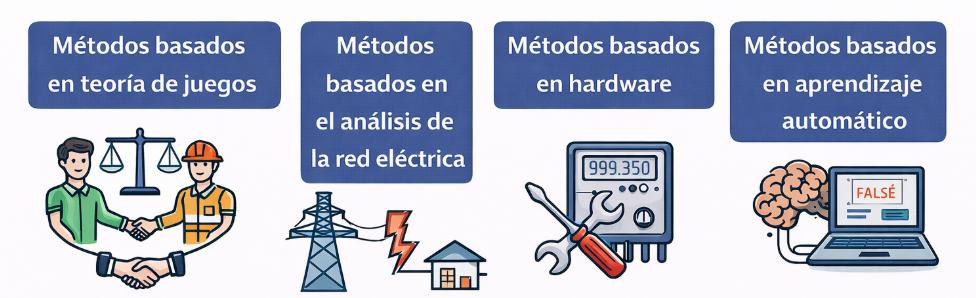
\includegraphics[width=0.95\textwidth]{imagenes/metodos.png}
    \caption{Métodos de detección de fraude eléctrico.}
\end{figure}

\subsubsection{Métodos basados en teoría de juegos}

De acuerdo con \cite{articulo1}, la teoría de juegos es una rama de estudio basada en el proceso de tomar decisiones interactivas entre agentes que compiten entre sí. En la detección del robo de electricidad, proporciona un método nuevo para analizar cómo interactúan las compañías eléctricas con los consumidores fraudulentos, lo que permite un análisis racional y sistemático de sus conductas. Todos los participantes se comportan racionalmente y persiguen maximizar su beneficio personal. Las compañías tratan de maximizar la tasa de detección y minimizar los costos operativos de las actividades de control e inspección, mientras que los ladrones intentan reducir al mínimo la probabilidad de ser atrapados con el fin de robar la mayor cantidad posible de energía. El robo es un juego estratégico en el que cada parte modifica su conducta en función de la otra. Esta categoría se caracteriza porque brinda una sólida base teórica y colabora en la creación de estrategias de detección y disuasión más eficaces. Al examinar sus limitaciones fundamentales, se puede notar que necesita suposiciones robustas acerca de la conducta de los actores, que es difícil elaborar funciones de utilidad realistas y que su implementación práctica es bastante limitada.


\subsubsection{Métodos basados en el análisis de la red eléctrica}

Los métodos de análisis de la red eléctrica buscan comportamientos que no son normales de consumo a través de analizar parámetros físicos del sistema eléctrico, tales como corrientes, voltajes, flujos de potencia y estados de la red. Para diferenciarlos de los métodos basados en datos históricos de consumo, estos métodos se basan en el modelo físico y operativo de la red de distribución. Se utilizan varias fuentes de información como datos de la red, datos de sensores e información recolectada por unidades terminales remotas y otros dispositivos de medición. Según el artículo \cite{articuloAnálisisRedEléctrica}, estos métodos detectan el robo de electricidad mediante el cálculo del sesgo, \emph{bias}, entre los valores estimados obtenidos a partir de modelos eléctricos, y los valores medidos por los dispositivos de la red. Calculan la diferencia entre lo que el sistema eléctrico debería consumir, valor estimado, y lo que los medidores realmente registran, valor medido. Este sesgo se compara con un umbral predefinido, cuanto mayor es la diferencia, mayor es la probabilidad de que exista robo de electricidad. Para estimar las pérdidas no técnicas conviene realizar un balance energético entre la energía suministrada por el transformador de distribución, y la suma de las lecturas de todos los medidores conectados. Si las pérdidas de línea superan un cierto umbral, se sospecha de consumo anómalo. Sin embargo, este método no distingue entre pérdidas técnicas y no técnicas, por lo que no resulta suficiente en escenarios reales complejos.

Esta categoría se divide en dos subcategorías: métodos basados en estimación de estado y métodos basados en análisis de flujo de potencia. La estimación de estado es una técnica fundamental en los sistemas eléctricos utilizada para estimar magnitudes de voltaje en los nodos y ángulos de fase a partir de datos medidos y del modelo de la red. Además de las mediciones tradicionales, estos métodos pueden incorporar: datos de sensores, mediciones de RTU o RFID, o parámetros eléctricos de la red (resistencias e inductancias) con el objetivo de mejorar la precisión de la detección. Para matizar, es importante distinguir RFID, identificación por radiofrecuencia, de RTU, Unidad Terminal Remota. Según el artículo \cite{{articuloRedEléctrica}}, sobre la estimación de estado en corriente alterna, las relaciones entre flujos de potencia, voltajes y ángulos son no lineales, y se expresan como:
\[z = h(x) + e,\]
donde $z$ es el vector de medidas, que puede incluir potencias activas y reactivas inyectadas, flujos de potencia y magnitudes de tensión; $x$ es el vector de estado, compuesto por las magnitudes de tensión y los ángulos de fase en los nodos del sistema; $h(x)$ representa el conjunto de funciones no lineales que relaciona el estado con las medidas; y $e$ es el vector de errores de medida. A partir de este modelo, la estimación del estado se formula como un problema de optimización basado en mínimos cuadrados ponderados, cuyo objetivo es minimizar la diferencia entre las medidas observadas y las estimadas:
\[J(\hat{x}) = (z - h(\hat{x}))^{T} W (z - h(\hat{x})),\]
donde $\hat{x}$ es el estado estimado y $W$ es una matriz diagonal de ponderación, cuyos elementos dependen de la precisión de las mediciones. La solución se obtiene mediante un proceso iterativo, que actualiza el estado estimado hasta que la diferencia entre iteraciones consecutivas es menor que el umbral de convergencia. Los métodos de análisis de flujo de potencia se basan en el principio de balance energético. Según este principio:
\[\text{Energía de entrada} \approx \text{Energía facturada} + \text{Pérdidas técnicas} + \text{Pérdidas no técnicas},\]
Si $E$ es la energía medida por el colector, dispositivo o sistema que recoge y agrega las mediciones de consumo eléctrico de varios usuarios, $e_i(t)$ como el consumo del usuario $i$ en el instante $t$, y $N$ como el número de usuarios, entonces:
\[E \approx \sum_{i=1}^{N} e_i(t) + l_t + \delta_t,\]
donde $l_t$ representa las pérdidas no técnicas (incluyendo robo de electricidad) y $\delta_t$ representa las pérdidas técnicas. La principal limitación de esta subcategoría es que no se puede localizar con precisión al usuario fraudulento.

\subsubsection{Métodos basados en \emph{hardware}}

Los métodos basados en \emph{hardware} se centran en el diseño de dispositivos físicos y estrategias de inspección para detectar o prevenir el robo de electricidad, dependiendo de equipamiento específico desplegado en la red eléctrica. Según el artículo \cite{articulo1}, estos métodos se dividen en tres categorías principales: desarrollo de dispositivos antirrobo, algoritmos de inspección basados en métodos de búsqueda y estrategias de despliegue de dispositivos de detección.

El desarrollo de dispositivos antirrobo de electricidad se centra en el diseño de equipos de medición o dispositivos especializados capaces de detectar o impedir la manipulación ilegal. En el último artículo mencionado se destaca que existen pocos estudios académicos en este ámbito, principalmente por dos razones. Los medidores inteligentes actuales ya incorporan varios mecanismos de antimanipulación, lo que reduce la necesidad de nuevos diseños y el desarrollo de nuevos dispositivos suele ser realizado por empresas privadas, cuyos diseños no se publican por motivos comerciales. Los medidores inteligentes utilizan varias técnicas para prevenir y detectar fraude, entre ellas destacan: el sellado físico o interruptores internos que alertan al microcontrolador ante accesos no autorizados, la prevención de manipulación magnética, reemplazando transformadores de corriente por bobinas de Rogowski y la detección de \emph{bypass} de corriente. Estos mecanismos son efectivos contra muchos métodos tradicionales de robo, pero la detección de fraudes sofisticados sigue siendo una lucha continua y cíclica, lo que fomenta la necesidad de desarrollar dispositivos más avanzados.

Los algoritmos de inspección basados en métodos de búsqueda tienen como objetivo encontrar medidores manipulados dentro de una red de área vecinal (NAN) en el menor tiempo posible. Existen dispositivos de búsqueda llamados inspectores, estos están formados por un inspector principal, que detecta comportamientos anómalos a nivel agregado y varios subinspectores, que ayudan a buscar los medidores afectados. La conexión entre medidores y subinspectores puede reconfigurarse sin afectar el suministro eléctrico. Si se sospecha que una NAN contiene usuarios fraudulentos, una inspección secuencial requeriría revisar todos los medidores en el peor de los casos. Los algoritmos de inspección reducen significativamente este tiempo mediante la comparación periódica entre lecturas agregadas de los subinspectores, y la suma de lecturas reportadas por los medidores. Además, del uso de estructuras lógicas para descartar rápidamente grupos de medidores sin necesidad de inspeccionarlos individualmente. Las estrategias para desplegar los dispositivos de detección buscan optimizar la ubicación y el número de dispositivos de monitoreo con el objetivo de reducir costes sin comprometer la capacidad de detección.


\subsubsection{Métodos basados en aprendizaje automático}

Los métodos basados en aprendizaje automático se utilizan para analizar los datos históricos de consumo eléctrico de los clientes, junto con información adicional, para detectar comportamientos anómalos relacionados con el robo de electricidad. Según el artículo \cite{articulo1}, estos métodos se clasifican en tres grandes grupos: aprendizaje supervisado, aprendizaje no supervisado y aprendizaje semi supervisado.

\medskip

\textbf{Aprendizaje supervisado}

El aprendizaje supervisado de acuerdo con el análisis de \cite{ML Supervisado} consiste en entrenar un modelo a partir de datos etiquetados, donde cada muestra de entrada x tiene asociada una etiqueta y. El objetivo es aprender una función: $f($x$)$ : $x$ → $y$, capaz de predecir correctamente la etiqueta de nuevos datos no vistos. Dado un conjunto de entrenamiento:
\[\{(x_1, y_1), (x_2, y_2), \dots, (x_N, y_N)\},\]
El modelo se entrena minimizando la función de pérdida esperada:
\[f(x) = \arg \min_{\hat{f}} {E}_{x,y}[L(y, \hat{f}(x))],\]
donde: $L(\cdot)$ es la función de pérdida. Las variables de entrada suelen ser lecturas de medidores inteligentes y características derivadas, mientras que la variable de salida es binaria: $y = 1$: usuario ilegal, $y = 0$: usuario legítimo.

Las tareas de aprendizaje supervisado se pueden dividir en problemas de clasificación y regresión. La clasificación, en los métodos de aprendizaje automático, utiliza un algoritmo para clasificar los datos en categorías, reconoce entidades específicas dentro del conjunto de datos e intenta determinar cómo se deben etiquetar o definir esas entidades. Algunos de los algoritmos más comunes son los clasificadores lineales, las máquinas de vectores de soporte (SVM), los árboles de decisión (DT), el k vecino más cercano (KNN), la regresión logística y el bosque aleatorio (RF). La regresión se usa para comprender la relación entre variables dependientes e independientes. En los problemas de regresión, el resultado es un valor continuo y los modelos intentan predecir el output objetivo. Algunos ejemplos son: la regresión lineal, la regresión de Lasso, la regresión de cresta y la regresión polinomial. El aprendizaje por conjuntos es un metaenfoque del aprendizaje supervisado en el que se entrenan varios modelos en la misma tarea de clasificación o regresión. Los resultados de todos los modelos del grupo se agregan para descubrir la mejor estrategia general para resolver el desafío.

Los modelos supervisados tradicionales poseen limitaciones que son analizadas en el artículo \cite{articulo1} tales como una dificultad para manejar datos de alta dimensionalidad, estos métodos son muy dependiente del conocimiento de un experto, tienen una baja capacidad para distinguir entre robo e irregularidades legítimas y, a veces, pueden ignorar la naturaleza temporal de los datos de consumo. Debido a estas limitaciones se motiva el uso de \emph{deep learning} mediante las redes neuronales. Estas, destacan en el manejo de problemas complejos de clasificación. Una red neuronal es una arquitectura de \emph{deep learning} que procesa datos de entrenamiento con capas de nodos que imitan el cerebro humano. Cada nodo se compone de entradas, ponderaciones, un sesgo y una salida. Si un valor de salida supera un umbral o sesgo preestablecido, el nodo se activa, pasando datos a la siguiente capa de la red.

Las principales técnicas supervisadas aplicadas a la detección de robo de electricidad, que se estudian en algunos de los trabajos de la literatura con más relevancia son: Modelos clásicos como SVM, DT, regresión lineal y logística, KNN y \emph{Naïve Bayes}, Métodos ensamble como RF, \emph{Gradient Boosting}, \emph{AdaBoost}, \emph{XGBoost} y \emph{Stacking} y, por último, destacan las redes neuronales, entre ellas el perceptrón multicapa (MLP), redes neuronales convolucionales (CNN), redes neuronales recurrentes (RNN, LSTM, GRU), \emph{autoencoders} (AE) y redes generativas adversarias (GAN).

\medskip

\textbf{Aprendizaje no supervisado}

El aprendizaje no supervisado en base a \cite{ML No Supervisado}, permite extraer patrones y estructuras a partir de datos sin etiquetar, lo que resulta especialmente útil en la detección de robo de electricidad, ya que este problema puede formularse como uno de detección de anomalías. En muchos escenarios reales y varios trabajos vistos, las etiquetas de usuarios fraudulentos no están disponibles debido a restricciones legales, de privacidad o de costos de inspección. Su principal objetivo es analizar correlaciones entre los perfiles de consumo individuales y variables agregadas e identificar patrones atípicos mediante técnicas de agrupamiento y detección de valores atípicos. Estos modelos se utilizan para tres tareas principales: \emph{clustering}, correlación y reducción de la dimensionalidad. A continuación se define cada método de aprendizaje y destacaremos los algoritmos y enfoques comunes para llevarlos a cabo con eficacia.

El \emph{clustering} es una técnica de minería que agrupa datos no etiquetados en base a sus similitudes o diferencias. Sus algoritmos, en el caso de la detección de fraude eléctrico, se utilizan para agrupar clientes con perfiles de consumo similares, aquellos grupos con pocos elementos o perfiles poco regulares se consideran \emph{outliers} y, por tanto, sospechosos. Los algoritmos de clustering se pueden clasificar en varios tipos: exclusivos, superpuestos, jerárquicos y probabilísticos. El exclusivo es una forma de agrupación que estipula que un punto de datos sólo puede existir en un clúster. Mientras que la superposición de clústeres se diferencia en que permite que los puntos de datos pertenezcan a varios clústeres con distintos grados de pertenencia. El jerárquico es un algoritmo de clustering sin supervisión que se puede clasificar de dos maneras: aglomerativo o divisivo. El aglomerativo se considera un “enfoque ascendente”. Sus puntos de datos se aíslan inicialmente como agrupaciones separadas y luego se fusionan iterativamente en función de la similitud hasta lograr un clúster. Y el clustering divisivo, adopta un enfoque descendente, un único clúster de datos se divide en función de las diferencias entre los puntos de datos. Para terminar con el \emph{clustering}, el probabilístico se basa en que los puntos de datos se agrupan en función de la probabilidad de que pertenezcan a una distribución determinada. El modelo de mezcla gaussiana (GMM) es uno de los métodos de clustering probabilístico más utilizados.

Una regla de correlación o asociación es un método basado en reglas para encontrar relaciones entre variables en un conjunto de datos determinado. Para analizar esta regla de correlación se emplean métodos para cuantificar la relación entre: consumo individual, consumo agregado, pérdidas no técnicas y mediciones eléctricas adicionales. Cuando la cantidad de dimensiones o características en un conjunto de datos es excesiva, se emplea una técnica llamada reducción de dimensionalidad. Reduce la cantidad de entradas de datos a un tamaño que sea manejable y, simultáneamente, conserva la integridad del conjunto de datos tanto como sea posible. La alta dimensionalidad se vuelve un desafío difícil de afrontar debido a la creciente resolución temporal de los datos que provienen de medidores inteligentes. Se aplican métodos de reducción de dimensionalidad, como la descomposición en valores singulares, el análisis de componentes principales y los autocodificadores con el objetivo de mitigar este problema.

El análisis de componentes principales (PCA) es un algoritmo que se emplea para disminuir la dimensionalidad, con el objetivo de eliminar duplicados y comprimir conjuntos de datos a través de la extracción de características. La descomposición en valores singulares (SVD) es un método distinto de reducción de dimensionalidad que fracciona una matriz A en tres matrices con rango reducido. La fórmula A = USVT, en la que $U$ y $V$ son matrices ortogonales, es la que representa el SVD. Los valores de la matriz $S$ son considerados como los valores singulares de la matriz $A$, y esta última es una matriz diagonal. Los autocodificadores utilizan las redes neuronales para la compresión de datos y, posteriormente, para generar una nueva representación de los datos originales.

Las principales técnicas no supervisadas que se aplican a la detección de robo de electricidad son: Redes bayesianas, Análisis de correlación, Técnicas de \emph{clustering}, Métodos basados en entropía, Inferencia difusa, Algoritmos de detección de \emph{outliers}, \emph{Optimum-Path Forest} (OPF), Análisis de Componentes Principales (PCA) y Teoría de matrices aleatorias. Estos métodos pueden generar falsos positivos, ya que son sensibles a la selección de umbrales y tienen dificultades para detectar ataques que imitan patrones normales. Debido a estas limitaciones se promueve el uso de enfoques intermedios como el aprendizaje semisupervisado.

\medskip

\textbf{Aprendizaje semisupervisado}

El aprendizaje semisupervisado, según la información de \cite{ML Semisupervisado}, utiliza lo más útil del aprendizaje supervisado y del no supervisado, aprovechando una cantidad pequeña de datos etiquetados y un alto volumen de datos sin etiquetar. Para entrenar modelos de inteligencia artificial en tareas de clasificación y regresión, se usan datos etiquetados y no etiquetados. Sus métodos son muy útiles cuando se trata de situaciones en las que obtener una cantidad apropiada de datos etiquetados es difícil o costoso, mientras que adquirir grandes cantidades de datos no etiquetados es más fácil. En estos casos, las técnicas de aprendizaje no supervisado y supervisado no proporcionarán soluciones adecuadas. La diferencia principal entre el aprendizaje semisupervisado y el supervisado es que, este último solo puede ser entrenado con conjuntos de datos completamente etiquetados, y el primero, también puede usar conjuntos de datos etiquetados como no etiquetados. Los algoritmos de aprendizaje no supervisados se distinguen por no aplicar datos etiquetados ni funciones de pérdida. El aprendizaje no supervisado impide que se produzcan situaciones que hagan posible la evaluación y perfeccionamiento del modelo.


\subsection{Conjuntos de datos para detección de fraude eléctrico}
En la literatura de la detección de fraude eléctrico mediante técnicas de aprendizaje automático, los conjuntos de datos usados tienen características diferentes dependiendo su procedencia, accesibilidad y estructura. Se pueden clasificar en varias categorías principales, en base al análisis de diferentes trabajos. La disponibilidad de datos públicos que posibilitan la evaluación y el entrenamiento reproducible de modelos es uno de los principales problemas. Algunas investigaciones emplean conjuntos de datos a los que se puede acceder públicamente y que contienen etiquetas claras de fraude, lo cual hace más sencillo el uso de métodos de aprendizaje supervisado. El \textit{Theft Detection Dataset (TDD2022)} es uno de ellos y es empleado en varios trabajos como \cite{articulo1} y \cite{articulo2}. Esta colección de datos incluye registros eléctricos con una frecuencia por hora durante cerca de un año; cada caso tiene una etiqueta que señala si el consumo es normal o está relacionado con uno de los seis tipos de fraude existentes, numerados del 1 al 6.

\begin{figure}[H]
    \centering
    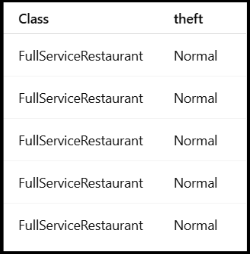
\includegraphics[width=0.75\textwidth, trim=0 15 0 0, clip]{imagenes/tabla_clases.png}
    \caption{Ejemplo de clases asociadas a cada registro.}
    \label{fig:tabla_clases}
\end{figure}

En la Figura~\ref{fig:tabla_clases} se puede ver un ejemplo del conjunto de datos. Este permite que cada registro represente un instante concreto, lo que lo hace adecuado para aprendizaje \emph{offline} como para aprendizaje \emph{online}. En ambos trabajos referenciados, este conjunto se emplea junto con esquemas de evaluación \emph{prequential}, test-then-train, en los que el modelo realiza una predicción sobre cada nueva instancia antes de ser actualizado con ella. Este tipo de evaluación es importante sobre todo en entornos dinámicos, aunque puede presentar limitaciones. Otra categoría importante corresponde a los conjuntos de datos reales proporcionados por compañías eléctricas. Estos reflejan comportamientos de consumo auténticos, lo que los convierte en una fuente de información muy valiosa para la detección de fraudes. Debido a las limitaciones de seguridad y privacidad, en muchos casos estos datos no son accesibles al público. La comparación de resultados con otros estudios es compleja, ya que ciertos trabajos analizados como \cite{articulo3} y \cite{articulo5} emplean este tipo de datos sin etiquetar o con un etiquetado restringido. Algunos estudios, como \cite{articulo4}, eligen crear conjuntos de datos simulados basándose en patrones de consumo habituales, debido a la falta de datos reales etiquetados. En estas situaciones, se introducen de manera artificial diversas formas de fraude para generar escenarios controlados que posibiliten la capacitación de modelos supervisados.

Tras analizar todos los grupos de conjuntos de datos que se utilizan para detectar el fraude eléctrico, es posible notar que, sin importar su procedencia, suelen tener una serie de propiedades comunes. Se trata de datos de series temporales que vienen de contadores inteligentes. En este caso, cada instancia refleja el consumo de electricidad en un espacio temporal específico. Asimismo, es común que estos conjuntos tengan un gran desequilibrio entre clases, con los casos de fraude siendo mucho menos comunes que los consumos normales. Esta particularidad tiene un impacto directo en la efectividad de los modelos y requiere el empleo de métricas concretas, como el estadístico Kappa o la puntuación F1. Por otra parte, la ausencia de datos públicos ampliamente aceptados complica la comparación entre distintos enfoques; esto representa uno de los retos más importantes en este campo. Conforme a estos rasgos, se escoge un conjunto de datos públicos que cuentan con etiquetas y una estructura temporal, lo cual permite la implementación de métodos de aprendizaje supervisado y el análisis del desempeño de los modelos en escenarios\emph{online} y \emph{offline}.


\section{Alcance}

El proyecto se fundamenta en el análisis, la implementación y la comparación de técnicas de aprendizaje automático que se utilizan para detectar fraudes en el consumo de electricidad. Su estructura se divide en diferentes secciones, como el análisis del estado del arte, donde se lleva a cabo un estudio de las metodologías empleadas en proyectos o artículos de internet relacionados con el fraude eléctrico. Incorpora procedimientos tradicionales de aprendizaje supervisado, técnicas para identificar patrones poco comunes y métodos de aprendizaje en línea. Se examinan diversas bases de datos públicas disponibles relacionadas con el uso de electricidad, que están etiquetadas por usuarios con fraude/no fraude o sin etiquetar, como parte del análisis de fuentes de datos.

En el estudio e implementación de métodos se seleccionan e implementan distintas técnicas de aprendizaje automático que se diferencian en \emph{offline} o \emph{online}. La idea, en un principio, era de 10 técnicas en total, 5 para cada opción. Finalmente, se implementó una \emph{offline} más que es esencial para este trabajo, debido a su mejor rendimiento en comparación al resto. La evaluación y comparación de métodos que realiza una comparativa entre los enfoques \emph{offline} y \emph{online} analizando, la capacidad de detección de fraude, la robustez ante datos desbalanceados, la adaptabilidad a cambios en el patrón de consumo y el coste computacional. El objetivo es determinar qué tipo de técnica resulta más adecuada según el escenario, histórico o en tiempo real.

A continuación, el diseño e implementación del prototipo, se desarrolla un entorno web que a través de los datos recogidos históricamente(\emph{offline}) o en tiempo real(\emph{online}) podrá simular un escenario real de detección de fraude eléctrico. El sistema permite simular consumo electrico, aplicar los métodos entrenados, mostrar resultados de la mejor técnica para \emph{offline} y \emph{online} en base a rendimiento, y comparar visualmente los enfoques \emph{online} y \emph{offline}. Este prototipo facilitará la escalabilidad y la incorporación futura de nuevos métodos. Para finalizar, se presentan las conclusiones obtenidas a partir del estudio comparativo, identificando fortalezas y debilidades de cada enfoque, y proponiendo posibles mejoras.


\section{Objetivo}

El propósito principal es diseñar e implementar un sistema de detección de fraude en el consumo eléctrico que emplee métodos de aprendizaje automático, aplicado a un conjunto particular de datos. Que permite comparar los modelos de aprendizaje \emph{offline} con los modelos de aprendizaje \emph{online}. Los siguientes objetivos específicos se sugieren para alcanzar esta meta general: implementar seis métodos relevantes de aprendizaje \emph{offline}; aplicar cinco métodos importantes de aprendizaje \emph{online}; analizar ambos grupos de modelos con métricas adecuadas; determinar la técnica más eficaz en cada categoría y añadir los modelos seleccionados a un prototipo de software que permita comparar visualmente los resultados y las métricas. En el sistema desarrollado debe poder analizar el comportamiento de los modelos en un entorno controlado, facilitando la comparación objetiva entre modelos \emph{online} y \emph{offline}.


\section{Glosario de Términos}

\begin{itemize}
\item \emph{Machine Learning} (Aprendizaje Automático): Campo de la inteligencia artificial que permite a los sistemas aprender patrones a partir de datos y realizar predicciones o clasificaciones sin estar programados para cada tarea concreta.

\item \emph{Dataset} (Conjunto de datos): Colección estructurada de datos utilizada para el entrenamiento, validación y evaluación de modelos de aprendizaje automático.

\item Métodos \emph{Offline}: Técnicas de aprendizaje automático en las que el modelo se entrena utilizando el conjunto completo de datos históricos antes de realizar predicciones, sin actualizarse durante la fase de explotación.

\item Métodos \emph{Online}: Técnicas de aprendizaje automático que actualizan el modelo de forma progresiva a medida que llegan nuevos datos, permitiendo su adaptación a flujos continuos de información.

\item \emph{Smart Grid} (Red Inteligente):  Sistema eléctrico que integra tecnologías digitales para monitorizar y gestionar de forma eficiente la generación, distribución y consumo de energía.

\item Evaluación \emph{Prequential}: Metodología de evaluación utilizada en aprendizaje \emph{online} donde cada instancia se utiliza primero para evaluar el modelo y posteriormente para actualizarlo.

\item Clasificación Supervisada: Técnica de aprendizaje automático en la que el modelo se entrena utilizando datos etiquetados para predecir la clase de nuevas instancias.

\item Métodos Ensamble: Técnica avanzada de aprendizaje automático que combina las predicciones de múltiples modelos individuales para crear un único modelo final más sólido, preciso y estable.

\item Modelo baseline: Modelo de referencia simple y rápido de construir para establecer un punto de partida, de forma que sirva para evaluar el rendimiento de modelos más complejos

\item Validación cruzada: Técnica utilizada en aprendizaje automático para evaluar el rendimiento y la capacidad de generalización de un modelo utilizando diferentes particiones del conjunto de datos.

\item \emph{One-Hot Encoding}: Técnica de preprocesamiento de datos utilizada en aprendizaje automático para convertir variables categóricas en variables numéricas que puedan ser utilizadas por los algoritmos de aprendizaje automático.

\item Validación cruzada estratificada: Técnica de aprendizaje automático utilizada para evaluar el rendimiento de un modelo, asegurando que cada pliegue, \emph{fold}, de datos mantenga la misma proporción de clases que el conjunto de datos original.
\end{itemize}


\section{Organización del documento}

En esta sección se presenta un resumen del contenido descrito en cada capítulo en los que está estructurado este documento. Se divide en tres grandes bloques: Prolegómeno, Desarrollo y Epílogo. El Prolegómeno se divide en: la introducción, explicación general acerca del proyecto y el estado del arte, y a parte, la planificación que incluye la metodología de desarrollo, planificación temporal, costes, riesgos y calidad. 

El Desarrollo está formado por: la elección y justificación de los datos en los que se basa el trabajo, es decir, el conjunto de datos con el que se trabaja; las técnicas usadas que incluyen la justificación de la elección de clasificación supervisada, comparación entre métodos y la elección y estudio de los métodos de aprendizaje automático; las métricas utilizadas para evaluar los resultados de las técnicas y la experimentación que incluye la implementación y configuración de los modelos, los resultados, análisis y conclusiones de los resultados.

El Epílogo se divide en: requisitos, análisis, diseño, construcción y pruebas del sistema. También recoge las conclusiones finales del proyecto donde se resumen los objetivos alcanzados, las lecciones aprendidas durante el desarrollo y se proponen posibles mejoras o trabajo futuro. Además, en el documento se incluyen un par de anexos. Apéndice A que recoge toda la lista completa de paquetes de Python instalados mediante pip, y apéndice B que detalla la información necesaria para el correcto uso de la web por parte del usuario incluyendo una descripción paso a paso para realizar adecuadamente cada una de las funcionalidades.


% =========================
% CAPÍTULO 2
% =========================
\chapter{Planificación}

\vspace{-1cm}

En esta sección se describen todos los aspectos relacionados a la gestión del proyecto: la metodología utilizada, la planificación, los costes, los riegos, el aseguramiento de la calidad y el análisis.


\section{Metodología de desarrollo}

La metodología iterativa e incremental se utiliza para ejecutar el proyecto, lo cual es apropiado para proyectos que a la vez desarrollan un entorno web y realizan investigación en aprendizaje automático. El desarrollo se ha dividido en dos bloques principales: Por un lado, el desarrollo del sistema, que abarca la aplicación de cinco métodos de aprendizaje \emph{online} y seis procedimientos de aprendizaje \emph{offline}, además del desarrollo del \emph{backend web} que se ocupa de integrar estos modelos. Por otro lado, se examinaron y llevaron a cabo los once modelos que se implementaron utilizando métricas pertinentes al problema de detección de fraude. Tras esta evaluación, se eligieron los modelos de cada categoría que presentaron el mejor rendimiento. El sistema admite la ejecución de las once técnicas puestas en práctica, pero solamente se muestran en el entorno web los modelos con un rendimiento superior por categoría como referencia principal para el usuario. El proyecto consta de las fases que se indican a continuación: Evaluación del problema y análisis del estado actual, elección y estudio del conjunto de datos, selección e indagación de métodos de aprendizaje automático, diseño de la arquitectura del sistema web, implementación de los modelos \emph{offline}, implementación de los modelos \emph{online}, comparación y evaluación de resultados, determinación del modelo más adecuado por categoría, creación del entorno web y finalmente las pruebas del sistema. Esta organización ayuda a la conservación de una planificación ordenada, propia de un modelo estructurado, mientras se incluyen iteraciones durante la etapa experimental para cotejar y validar los modelos que se han implementado.


\section{Planificación del proyecto}

La planificación consta de varias etapas secuenciales y con iteraciones, debido a la metodología y el carácter mixto del proyecto, que integra la experimentación en aprendizaje automático con la creación de un entorno web. El análisis del problema incluye el estudio de la detección de fraude eléctrico, la revisión de técnicas actuales en el estado del arte y el examen del conjunto de datos elegido. La duración verdadera fue de tres semanas, mientras que la estimada era de cuatro. Se examinan distintos algoritmos de clasificación supervisada, incluyendo tanto los \emph{offline} como los \emph{online}, después de que el análisis, la investigación y la elección de técnicas de aprendizaje automático han concluido. Se eligen métodos de cada categoría según la problemática y la idoneidad para el conjunto de datos escogido. La duración estimada es de una semana, y la durabilidad concreta también es de una semana.

La implementación de los modelos se lleva a cabo incluyendo la aplicación de modelos \emph{offline}. Se emplean cinco métodos de aprendizaje \emph{offline}con el uso de bibliotecas especializadas y mediante la modificación de parámetros. La duración calculada es de dos semanas, pero la verdadera fue de tres a causa de dificultades en la optimización de alguno de los modelos. Para poner en práctica modelos \emph{online}, se emplean cinco métodos de aprendizaje \emph{online} mediante el uso de bibliotecas especializadas y la realización de ajustes a los parámetros. La duración real fue de dos semanas, al igual que la duración estimada. Luego de implementar los modelos, se procede a la evaluación comparativa de los mismos, para lo cual se elabora un protocolo estandarizado que emplea métricas idóneas para detectar fraudes. Se ponen en práctica los modelos bajo las mismas condiciones y se examinan los resultados. La duración real fue de dos semanas, al igual que la duración estimada. Además, del diseño e implementación del entorno web, se desarrolla la arquitectura de la web, incluyendo \emph{backend}, integración de modelos y visualización de resultados. La duración estimada y real son de cinco semanas. Por último,  las pruebas y validación del sistema, se realizan pruebas funcionales y no funcionales para garantizar el correcto funcionamiento del sistema y la integración entre componentes. Duración estimada 1 semana.


\subsection{Hitos principales}

Para definir los hitos principales del proyecto se dividen en función de los entregables técnicos más relevantes del sistema. Hito 1. Análisis y definición del problema: Revisión del estado del arte y selección del conjunto de datos TDD2022. Hito 2. Selección de técnicas y métricas: Elección de métricas de evaluación, elección de cinco técnicas de aprendizaje automático \emph{offline} y elección de cinco técnicas de aprendizaje automático \emph{online}. Hito 3. Implementación de modelos: Desarrollo de las cinco técnicas \emph{offline} seleccionadas, desarrollo de las cinco técnicas \emph{online} seleccionadas, ajuste de hiperparámetros y validación inicial de resultados. Hito 4. Evaluación comparativa y selección: Definición del protocolo común de evaluación, aplicación de evaluación tradicional para modelos \emph{offline}, aplicación de evaluación prequential para modelos \emph{online}, comparación mediante métricas adecuadas al problema y selección del mejor modelo \emph{offline} y del mejor modelo \emph{online}. Hito 5. Desarrollo del sistema web: Diseño de la arquitectura del backend, integración de los modelos seleccionados e implementación de endpoints y visualización de resultados. Hito 6. Pruebas y validación final: Pruebas funcionales, pruebas no funcionales y ajustes finales del sistema.


\subsection{Estimación temporal}

La estimación inicial del proyecto se realiza considerando las distintas fases de desarrollo y la naturaleza experimental del trabajo. Se estimó una dedicación aproximada de entre 300 y 330 horas para el proyecto. Además, sumándole las horas estimadas para la documentación un aproximado de 60 horas, da como resultado un total de entre 360 y 390 horas para el proyecto al completo. Sin embargo, esta estimación puede resultar inferior en comparación a la real debido a la complejidad del ajuste de modelos y la curva de aprendizaje asociada al desarrollo de técnicas \emph{online}. (Por comprobar al acabar el proyecto).


\subsection{Diagrama de Gantt}

\begin{figure}[H]
\centering
\makebox[\textwidth][c]{%
\begin{ganttchart}[
    hgrid,
    vgrid,
    x unit=0.7cm,
    y unit chart=0.6cm,
    bar height=0.6,
    group height=0.8
]{1}{16}

\gantttitle{2026}{16} \\
\gantttitle{Febrero}{4}
\gantttitle{Marzo}{4}
\gantttitle{Abril}{4}
\gantttitle{Mayo}{4} \\
\gantttitlelist{1,...,16}{1} \\

% PRELIMINARES
\ganttgroup[group/.append style={fill=blue!60}]{Preliminares}{1}{4} \\
\ganttbar[bar/.append style={fill=blue!30}]{Análisis de fuentes de datos}{1}{4} \\

% OFFLINE
\ganttgroup[group/.append style={fill=green!60}]{Técnicas offline}{4}{7} \\
\ganttbar[bar/.append style={fill=green!30}]{Estudio de técnicas de AA}{4}{4} \\
\ganttbar[bar/.append style={fill=green!30}]{Elección de métricas de evaluación}{4}{4} \\
\ganttbar[bar/.append style={fill=green!30}]{Implementación y entrenamiento}{5}{6} \\
\ganttbar[bar/.append style={fill=green!30}]{Comparativa}{7}{7} \\

% ONLINE
\ganttgroup[group/.append style={fill=orange!70}]{Técnicas online}{4}{10} \\
\ganttbar[bar/.append style={fill=orange!40}]{Estudio de técnicas de AA}{4}{4} \\
\ganttbar[bar/.append style={fill=orange!40}]{Elección de métricas de evaluación}{4}{4} \\
\ganttbar[bar/.append style={fill=orange!40}]{Implementación y entrenamiento}{8}{9} \\
\ganttbar[bar/.append style={fill=orange!40}]{Comparativa}{10}{10} \\

% PROTOTIPO
\ganttgroup[group/.append style={fill=purple!60}]{Prototipo}{11}{16} \\
\ganttbar[bar/.append style={fill=purple!30}]{Diseño de clases}{11}{11} \\
\ganttbar[bar/.append style={fill=purple!30}]{Implementación interfaz}{12}{14} \\
\ganttbar[bar/.append style={fill=purple!30}]{Integración de modelos}{15}{15} \\
\ganttbar[bar/.append style={fill=purple!30}]{Tests}{16}{16} \\

% MEMORIA
\ganttgroup[group/.append style={fill=red!60}]{Memoria}{3}{16} \\
\ganttbar[bar/.append style={fill=red!30}]{Redacción y documentación}{3}{16}

\end{ganttchart}
}
\caption{Diagrama de Gantt del proyecto.}
\end{figure}


\section{Costes}

Para determinar el precio total del proyecto, es necesario tomar en cuenta distintos factores, entre ellos el sueldo del ingeniero de informática responsable de diseñar el sistema, los gastos de la electricidad, los costos de la vivienda y la infraestructura, así como los costos de los materiales.

Respecto al componente humano, Randstad \cite{randstad} indica que los sueldos promedio de un ingeniero junior en informática en España oscilan entre los 22.000~\euro{} y 28.000~\euro{} anuales en el sector privado. Entonces, tomando el mínimo que son 22.000~\euro, ya que no tengo experiencia laboral, y jornada completa de 160 horas mensuales, es decir, 1920 horas anuales. El coste por hora es de aproximadamente 11.46~\euro/hora. Si el proyecto ha requerido aproximadamente 390 horas como se estimó como máximo, el coste del desarrollo será de 4469.40~\euro.

Para determinar el coste del consumo eléctrico, es necesario considerar el costo de la electricidad. Este se obtiene al calcular el consumo promedio de un ordenador de gama media, que es de 300 W/hora durante 5 horas diarias; el resultado es 1.5 KWh. Con un precio medio de la electricidad de 0.17~\euro/KWh, el coste diario de la jornada de trabajo es de aproximadamente 0.225~\euro/día, y el coste por hora será de 0.051~\euro/hora. El precio puede variar dependiendo el mercado y situaciones externas. Como el proyecto ha requerido aproximadamente 390 horas como se estimó como máximo, el coste del consumo eléctrico será de 19.89~\euro.

Es necesario considerar que el software empleado en la creación del proyecto es de código abierto y no tiene costo para determinar el precio del software. Por lo tanto, el precio final del software es de 0~\euro. Asimismo, es necesario considerar lo siguiente en cuanto al costo de la infraestructura y el alojamiento. El sistema se ha llevado a cabo en un entorno local durante el desarrollo, sin requerir servidores de pago externos.

En caso de despliegue real en producción, sería necesario considerar: Servidor cloud, he tomado la decisión de usar AWS, ya que como alumno de la UCA tengo acceso gratuito y Base de datos en la nube, he usado MySQL que es gratuito y de código abierto. Lo que hace un total de 0~\euro. Al ser un entorno acádemico se puede conseguir gratuito, pero si sale del entorno acádemico podría no serlo. También, como el equipo informático ya estaba disponible antes del desarrollo del proyecto, el coste real del material fue de 0~\euro. Por tanto, el coste total del proyecto sumando todos los costes es de 4489.29~\euro.


\section{Riesgos}

Dado que el proyecto combina una fase experimental de evaluación de modelos de aprendizaje automático con el desarrollo de un entorno web, los riesgos encontrados se centran en aspectos técnicos, metodológicos y de integración. Por tanto, ya que el proyecto se desarrolla íntegramente en un entorno software y no implica despliegue físico ni interacción con infraestructuras reales, no se tienen en cuenta riesgos físicos importantes. A continuación, se detallan los principales riesgos detectados en forma de cuadro.

\begin{table}[H]
\centering
\begin{tabular}{|p{5cm}|p{2.5cm}|p{2.5cm}|p{5cm}|}
\hline
\textbf{Descripción} & \textbf{Probabilidad} & \textbf{Impacto} & \textbf{Solución} \\
\hline

El conjunto de datos elegido presenta una distribución desigual entre las clases de fraude y no fraude, lo que puede provocar que los modelos presenten métricas altas pero con bajo rendimiento. 
& Media & Alto 
& Uso de métricas adecuadas y una comparación equilibrada entre modelos. \\
\hline

Las técnicas de aprendizaje automático online pueden presentar menor precision que los modelos offlines, sobre todo en conjuntos de datos complejos. 
& Media & Medio 
& Buen ajuste de hiperparámetros y una evaluación prequential adecuada. \\
\hline

Los modelos offlines podrían adaptarse en exceso a los datos de entrenamiento, reduciendo su capacidad de generalización. 
& Media & Alto 
& Correcta separación entre las fases de entrenamiento y de test. \\
\hline

La integración de los modelos seleccionados en el entorno web podría generar errores en la carga del modelo, tiempos de respuesta elevados o incompatibilidades entre librerías. 
& Media & Medio 
& Validación independiente antes de cada modelo y una realización de pruebas adecuadas. \\
\hline

El proyecto se basa en un único conjunto de datos público, lo cuál puede limitar la generalización de los resultados. 
& Alta & Medio 
& Explicación clara del conjunto de datos seleccionado. \\
\hline

\end{tabular}
\caption{Riesgos identificados y medidas de mitigación}
\end{table}


\section{Aseguramiento de calidad}

El aseguramiento de la calidad de este proyecto debe contemplar tanto la validez científica de los resultados como la robustez técnica del sistema implementado. Primero, se tienen en cuenta los distintos tipos de calidad. Calidad en la fase experimental, para garantizar que los resultados obtenidos en la comparativa entre modelos sean válidos, se aplican varias medidas: definición de métricas adecuadas, aplicación de un protocolo común de evaluación para todos los modelos, una clara separación entre datos de entrenamiento y pruebas en los modelos offline y el uso de evaluación prequential en modelos online. Calidad del código y desarrollo software, durante el desarrollo del sistema web se aplican buenas prácticas de programación: Control de versiones, modularización del código, gestión estructurada de dependencias, documentación clara y pruebas. Y por último, calidad en la integración entre modelos y sistema, Antes de realizar la integración de los modelos seleccionados en el entorno web: Cada modelo se valida de manera independiente, se comprueban tiempos de inferencia, se verifica la correcta serialización y carga del modelo y se realizan pruebas de integración.

Además, debe de tener reproducibilidad, para que que los experimentos realizados puedan ser replicados bajo las mismas condiciones, obteniendo resultados consistentes y verificables, se dejan claro varios aspectos técnicos del proyecto: Uso de versiones concretas de librerías, definición del entorno virtual, documentación del proceso de ejecución y una estructura clara del proyecto. También, existen limitaciones de calidad debido a que el proyecto solo se basa en único conjunto de datos, los resultados obtenidos pueden estar condicionados por sus propias características específicas. Esto se reconoce y se discute sobre ello en las conclusiones.



% =========================
% PARTE II DESARROLLO
% =========================
\part{Desarrollo}


% =========================
% CAPÍTULO 3
% =========================
\chapter{Datos}

\section{Conjunto de datos seleccionado}

Para desarrollar este proyecto se trabaja con el conjunto de datos llamado Theft Detection Dataset (TDD2022), el cuál se encuentra disponible de manera pública a través de la plataforma Mendeley Data \cite{dataset}. Este, es el mismo mencionado anteriormente y contiene registros de consumo eléctrico obtenidos a partir de redes inteligentes. Además, incluye comportamientos normales y diferentes tipos de fraude eléctrico. Cada registro temporal se encuentra etiquetado con una clase asociada, de esta manera, permite diferenciar entre consumo legítimo y diversas formas de fraudes. Presenta varias características que justifican su elección para el desarrollo del presente trabajo. En primer lugar, destaca su disponibilidad pública, ya que es de los pocos conjuntos de datos que se encuentra disponible para su análisis y descarga de manera pública.  Además, cuenta con un etiquetado explícito de fraude, siendo el único encontrado que tiene una clara diferencia entre clases normales y fraudes, incluyendo una clasificación supervisada clara.  Por otra parte, presenta una adecuada estructura para aprendizaje \emph{online}, ya que además de poder utilizarse para técnicas \emph{offline}, al estar etiquetado por instancia temporal y presentar una estructura secuencial, resulta apropiado para técnicas \emph{online}. 

Se trata de un conjunto de datos de uso reciente, empleado en varios estudios actuales sobre detección de fraude eléctrico, como se analizó en la sección del estado del arte, lo que facilita la comparación con trabajos previos. También me gustaría destacar que, aunque este conjunto de datos proporciona un entorno controlado y bien estructurado para evaluación de métodos, su naturaleza parcialmente simulada puede no reflejar la complejidad de escenarios reales de fraude. A pesar de eso, representa una base muy sólida, estandarizada y adecuada para el análisis comparativo planteado en este proyecto y cumplir los objetivos propuestos.


% =========================
% CAPÍTULO 4
% =========================
\chapter{Técnicas}


\section{Clasificación supervisada para detección de fraude}

La detección de fraude eléctrico por medio de procedimientos de aprendizaje automático puede ser tratada de distintas formas, tal como se ha explicado en la sección sobre el estado del arte. El aprendizaje supervisado se distingue por su habilidad de manejar datos etiquetados y de aprender patrones relacionados con conductas que pueden ser fraudulentas. Se elige la clasificación supervisada en este trabajo porque el conjunto de datos seleccionado cuenta con etiquetas explícitas que hacen posible distinguir entre un consumo normal y uno fraudulento. Esto hace más sencillo el uso directo de modelos de clasificación y la evaluación objetiva de su desempeño a través de métricas. Estas métricas son examinadas y elegidas en partes subsiguientes. Además, ayuda a resolver el problema como una tarea binaria, donde el modelo tiene que decidir si un patrón de consumo específico tiene comportamientos normales o de fraude. Se usa mucho en los trabajos y proyectos en los que se usan distintos algoritmos, que se examinan y analizan en las siguientes secciones. En estos trabajos, la detección de fraude eléctrico ha tenido resultados positivos. En este trabajo, por lo tanto, se utilizan diversos modelos de clasificación supervisada con el propósito de comparar su eficacia en la identificación del fraude y examinar su actuación en situaciones \emph{online} y \emph{offline}.


\section{Comparación entre métodos \emph{offline} y \emph{online}}

Los modelos de aprendizaje automático utilizados se pueden dividir en dos grandes grupos según su forma de aprendizaje: métodos \emph{offline} y métodos \emph{online}. Los primeros se basan en el uso de conjuntos de datos históricos para la formación del modelo. El entrenamiento se lleva a cabo inicialmente con todos los datos existentes, y después se utiliza el modelo para hacer predicciones sin una actualización continua. Esto es apropiado si los datos son representativos y estáticos del problema, lo que permite alcanzar modelos estables con un rendimiento general adecuado. Lo malo, es que tienen restricciones en situaciones dinámicas, como el consumo de electricidad en redes inteligentes, donde los patrones de conducta pueden variar con el tiempo o instantáneamente. En estos casos, un modelo previamente entrenado podría dejar de ser capaz de hacer predicciones adecuadas si no se le incorpora información nueva.

Por otro lado, los métodos de aprendizaje \emph{online} permiten la actualización y el entrenamiento del modelo de forma gradual conforme se reciben nuevos datos. El modelo no se entrena solo una vez, sino que sigue aprendiendo y se ajusta a eventuales alteraciones en los patrones de consumo y en las conductas potencialmente fraudulentas. Esto es relevante en situaciones donde los datos se producen de manera secuencial, como sucede con los medidores inteligentes de electricidad. Una de las mayores ventajas es su habilidad para ajustarse a las variaciones temporales, lo que facilita la identificación de nuevas formas de fraude sin requerir el reentrenamiento del modelo desde el principio. Sin embargo, estos métodos suelen ser más difíciles de poner en práctica. A causa de estas discrepancias, en este estudio se propone comparar modelos online y offline con el fin de examinar su adaptabilidad, estabilidad y rendimiento. Esta comparación posibilitará determinar qué modelo de aprendizaje automático es más apropiado para identificar el fraude en el consumo de electricidad en un contexto real.


\section{Selección y Estudio de Técnicas de Aprendizaje Automático}

En esta sección se seleccionan y analizan los métodos de aprendizaje automático y las métricas consideradas más adecuados para el problema de detección de fraude en el consumo eléctrico. Además, cada categoría tendrá un modelo \emph{baseline} con el fin de tener un punto de referencia inicial que permita comparar el rendimiento de modelos más avanzados.


\subsection{Técnicas \emph{offline}}

En este trabajo, el problema se presenta como un caso de clasificación supervisada cuyo propósito es determinar si un patrón específico de consumo eléctrico es normal o fraudulento. Se eligen varias metodologías de aprendizaje automático \emph{offline}, o sea, modelos que se entrenan con un conjunto de datos históricos completo antes de ser valorados. Este modo permite analizar en profundidad el rendimiento de distintos algoritmos bajo condiciones controladas. La selección de estos modelos se realiza de una manera minuciosa atendiendo a varios criterios: su uso en la literatura científica en problemas de detección de fraude eléctrico, su capacidad para manejar datos desbalanceados y complejos, y la posibilidad de comparar diferentes paradigmas de aprendizaje dentro de un mismo problema.


\subsubsection{Regresión Logística}

La regresión logística es un modelo lineal ampliamente utilizado en problemas de clasificación binaria en trabajos como \cite{articuloBase}. Para explicar como funciona este modelo, se tiene que tener en cuenta que se basa en modelar la probabilidad de pertenencia a una clase mediante una función sigmoidea: $f(x) = \frac{1}{1 + e^{-x}}$, este modelo estima la probabilidad de que una instancia pertenezca a la clase positiva, fraude, a partir de una combinación lineal de las variables de entrada. Si se representa esta ecuación de regresión logística, se consigue una curva en S como la que se muestra en la figura a continuación.

\begin{figure}[H]
    \centering
    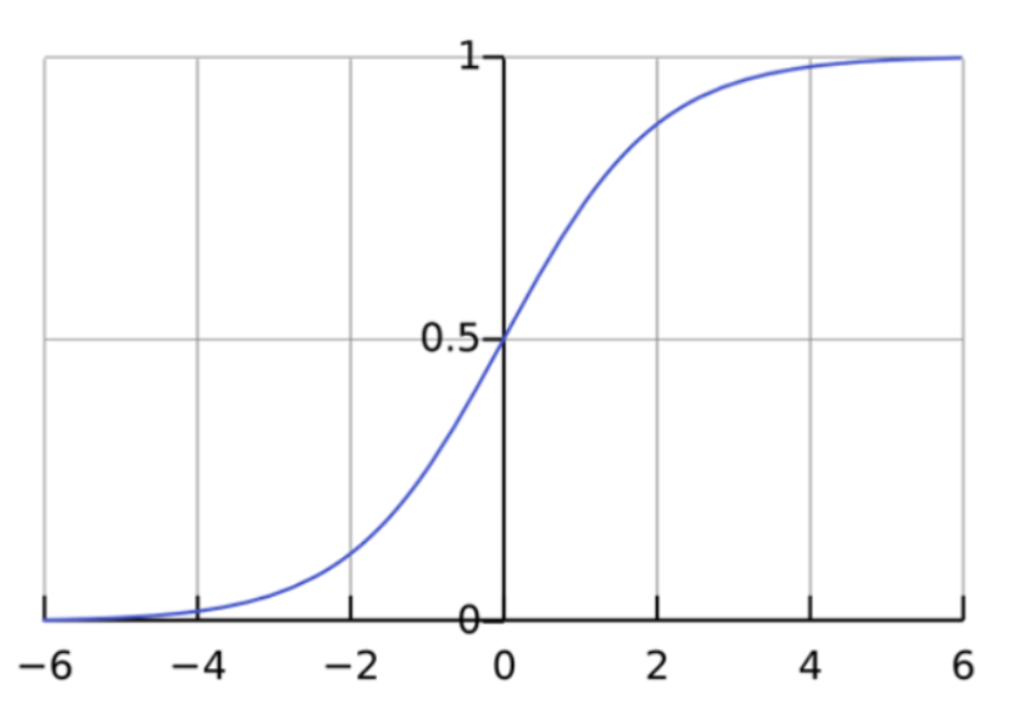
\includegraphics[width=0.6\textwidth]{imagenes/curva_sigmoidea.png}
    \caption{Curva sigmoidea de la regresión logística según \cite{logistic-regression}.}
\end{figure}

Teniendo los siguientes datos: Eje x es la variable de entrada o característica, el eje f(x) es la probabilidad estimada por el modelo y la curva muestra cómo cambia la probabilidad según el valor de entrada. La función solo devuelve valores entre 0 y 1 para la variable dependiente, al margen de los valores de la variable independiente. Así estima la regresión logística el valor de la variable dependiente. 

A pesar de su simplicidad, la regresión logística presenta importantes limitaciones en problemas complejos como la detección de fraude eléctrico, donde las relaciones entre variables suelen ser no lineales y altamente dependientes del contexto temporal y del tipo de consumo. Por este motivo, en este trabajo se utiliza como modelo \emph{baseline}. Su bajo coste computacional y facilidad de interpretación lo convierten en una herramienta útil para establecer una base sólida para los siguientes métodos.


\subsubsection{\emph{Random Forest}}

\emph{Random Forest}, bosque aleatorio traducido al español, es un algoritmo de aprendizaje supervisado, que usa múltiples árboles de decisión utilizado en trabajos como \cite{articuloBase}, \cite{articulo2} y \cite{articulo3}, donde en este último se incluye como técnica dentro de la revisión de los métodos existentes. Cada árbol se entrena sobre una muestra aleatoria del conjunto de datos y utiliza un subconjunto aleatorio de variables, lo que añade diversidad en el modelo. Se componen de tres hiperparámetros principales, que deben configurarse antes del entrenamiento. Son el tamaño del nodo, la cantidad de árboles y la cantidad de características muestreadas. A partir de ahí, el clasificador de bosque aleatorio se utiliza para resolver problemas de regresión o clasificación.

Su algoritmo se compone de una colección de árboles de decisión y cada árbol en el conjunto está compuesto por una muestra de datos extraída de un conjunto de entrenamiento con reemplazo, llamado \emph{bootstrapping}. De esa muestra de entrenamiento, un tercio de ella se reserva como datos de prueba, lo que se conoce como la muestra fuera de bolsa, \emph{oob}. Luego, se inyecta otra instancia de aleatoriedad mediante el embolsado de características, lo que agrega más diversidad al conjunto de datos y reduce la correlación entre los árboles de decisión. Dependiendo del tipo de problema, la determinación de la predicción variará. Para una tarea de regresión, se promediarán los árboles de decisión individuales, y para una tarea de clasificación, el voto mayoritario, es decir, la variable categórica más frecuente, arrojará la clase prevista. Finalmente, la muestra fuera de la bolsa se utiliza para la validación cruzada, finalizando esa predicción.

\begin{figure}[H]
    \centering
    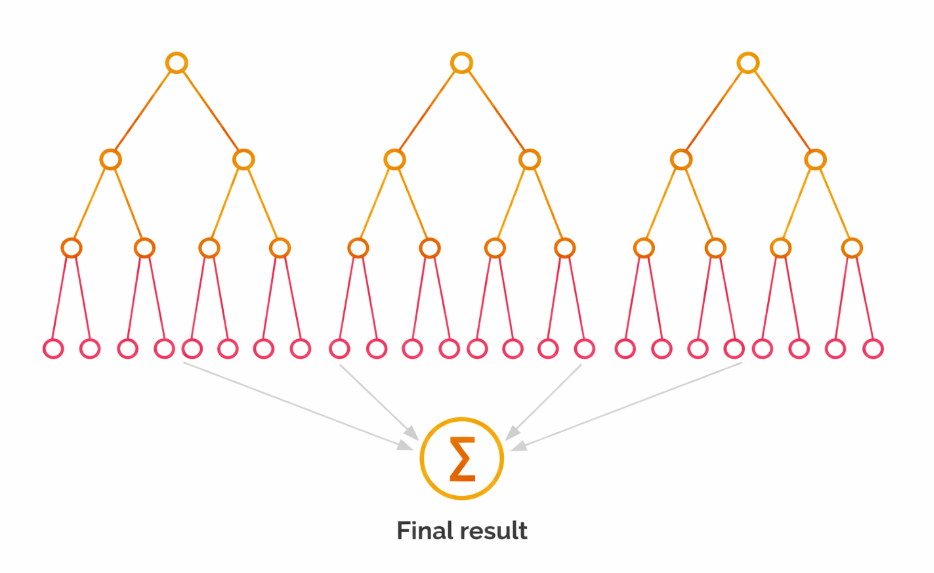
\includegraphics[width=0.8\textwidth]{imagenes/arboles.png}
    \caption{Árboles de decisión del algoritmo de Bosque Aleatorio según \cite{Random Forest}.}
\end{figure}

Este tipo de algoritmos es utilizado en la literatura para la detección de fraude eléctrico debido a su capacidad para capturar relaciones no lineales entre variables, manejar grandes volúmenes de datos y por ser robusto frente a ruido y datos desbalanceados, lo cuál es especialmente importante debido al conjunto de datos seleccionado. Además, este algoritmo permite obtener medidas de importancia de variables, lo que facilita la interpretación del modelo y la identificación de los factores más relevantes en la detección de fraude.


\subsubsection{\emph{Gradient Boosting}}

\emph{Gradient Boosting}, conocido es esnpañol como \emph{boosting} de gradiente, es un método de aprendizaje automático basado en técnicas ensamble que construye el modelo de forma secuencial. En este método cada modelo nuevo se entrena para corregir los errores cometidos por los modelos anteriores. El proceso consta de minimizar una función de pérdida mediante técnicas de optimización basadas en gradiente, lo que permite ajustar progresivamente el modelo a los datos. A continuación se va a explicar el funcionamiento de su algoritmo. Para empezar, se utiliza un conjunto de entrenamiento para establecer una base con un modelo base de aprendizaje, a menudo un árbol de decisión, cuyas predicciones iniciales se generan aleatoriamente. Normalmente, el árbol de decisión sólo contiene unos pocos nodos hoja, estos aprendices débiles sirven como un punto de partida óptimo. Esta configuración inicial allana el camino para que se desarrollen iteraciones posteriores. Después de la inicialización, para cada ejemplo de entrenamiento se calcula el error residual restando el valor previsto del valor real. Este paso identifica las áreas en las que es necesario mejorar las predicciones del modelo.

Después del cálculo residual y antes del entrenamiento de un nuevo modelo, tiene lugar el proceso de regularización. Esta etapa implica reducir la influencia de cada nuevo aprendiz débil integrado en el conjunto. Al calibrar cuidadosamente esta escala, se puede controlar la rapidez con la que avanza el algoritmo de \emph{boosting}, lo que ayuda a prevenir el sobreajuste y a optimizar el rendimiento general. A continuación, se utilizan los errores residuales calculados en el paso anterior como objetivos y se entrena un nuevo modelo o un aprendiz débil para una predicción con precisión. El objetivo de este paso es corregir los errores cometidos por los modelos anteriores, refinando la predicción general. Ahora vienen las actualizaciones del conjunto, el rendimiento del conjunto actualizado, incluido el modelo recién entrenado, se suele evaluar mediante un conjunto de pruebas independiente. Si el rendimiento de este conjunto de datos reservado es satisfactorio, el conjunto se actualiza incorporando el nuevo aprendiz débil; de lo contrario, podría ser necesario realizar ajustes en los hiperparámetros.

Cuando estén las actualizaciones del conjunto, se repiten los pasos presentados anteriormente según sea necesario. Cada iteración se basa en el modelo base y lo refina mediante el entrenamiento de nuevos árboles, lo que mejora aún más la precisión del modelo. Si la actualización del conjunto y el modelo final son satisfactorios en comparación con el modelo de referencia basado en la precisión, se continúa el proceso en el siguiente paso. Para terminar el proceso, se detiene el proceso de \emph{boosting} cuando se cumpla un criterio de detención predeterminado, como un número máximo de iteraciones, precisión objetivo o rendimientos decrecientes. Este paso ayuda a garantizar que la predicción final del modelo logre el equilibrio esperado entre complejidad y rendimiento.

\begin{figure}[H]
    \centering
    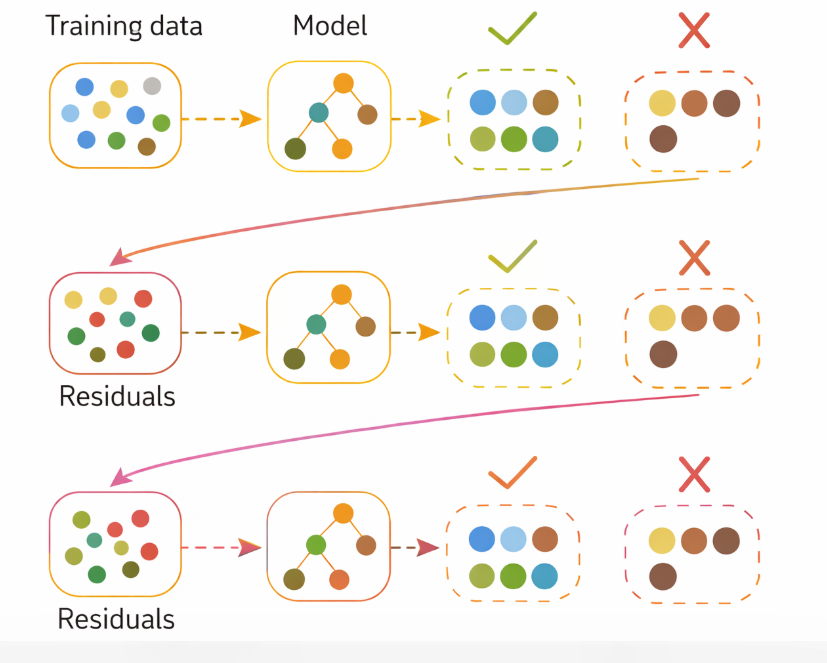
\includegraphics[width=0.8\textwidth]{imagenes/boosting.png}
    \caption{Proceso del \emph{Boosting} de gradiente según \cite{Gradient Boosting}.}
\end{figure}

Aunque no se encontró el uso de este algoritmo en estudios y trabajos similares, este presenta varias ventajas en el contexto de detección de fraude como la alta capacidad para modelar relaciones complejas, el buen rendimiento en datos desbalanceados y la mayor precisión en comparación con modelos individuales. Debido a estas características, los métodos de \emph{boosting} son frecuentemente utilizados en aplicaciones reales de detección de fraude. Como posible mejora, se emplea, en unas secciones más abajo, el uso de XGBoost, una versión optimizada del \emph{Gradient Boosting} ampliamente utilizada en problemas de detección de fraude y en trabajos como \cite{articulo3}.


\subsubsection{K vecinos más cercanos}

K vecinos más cercanos (KNN) es un algoritmo de aprendizaje automático utilizado en diversos trabajos como \cite{articulo1}, \cite{articulo2} y \cite{articuloBase}, donde en este último se utiliza como método de referencia para comparación. Está basado en instancias que clasifica nuevas observaciones en función de la clase mayoritaria entre sus vecinos más cercanos. Además, es uno de los métodos de clasificación y regresión más populares y sencillos que se emplean actualmente. Si bien el algoritmo se usa para problemas de regresión o clasificación, en este trabajo se utiliza como un algoritmo de clasificación, partiendo del supuesto de que se pueden encontrar puntos similares cerca uno del otro. La principal diferencia entre ambos es que la clasificación se emplea para valores discretos, mientras que en la regresión se emplea con valores continuos. Este método forma parte de una familia de modelos que sólo almacenan un conjunto de datos de entrenamiento en vez de hacer una fase de entrenamiento. Esto implica que todo el cálculo se produce cuando se realiza una clasificación o predicción.

\begin{figure}[H]
    \centering
    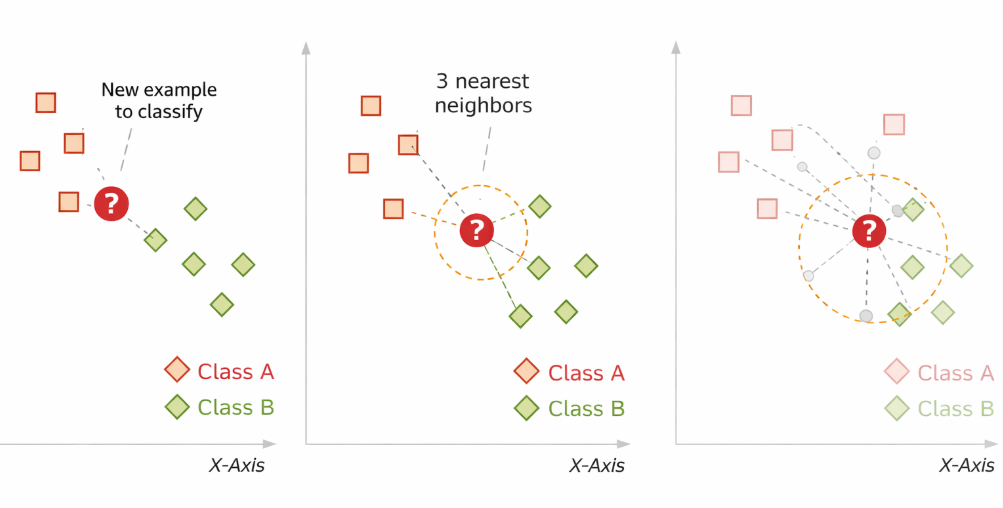
\includegraphics[width=0.8\textwidth]{imagenes/diagramaKNN.png}
    \caption{Diagrama KNN según \cite{k-Nearest Neighbors}.}
\end{figure}

Para observar cómo funciona este modelo hay que analizar cómo calcular las métricas de distancia y el valor $k$. Primero se explican las métricas, y luego, el valor $k$. Para empezar, se tiene que determinar qué puntos de datos están más cerca de un punto de consulta determinado. Para ello, será necesario calcular la distancia entre el punto de consulta y los demás puntos de datos. Esas métricas de distancia ayudan a formar límites de decisión, que dividen los puntos de consulta en diferentes regiones. Por lo general, los límites de decisión se visualizan con diagramas de Voronoi. A continuación se van a ver algunas de las medidas de distancia existentes.

La distancia euclídea ($p=2$) es la medida de distancia generalmente más usada y está limitada a vectores de valores reales. Empleando la siguiente fórmula, se mide una línea recta entre el punto de consulta y el otro punto que se está midiendo. Su fórmula es

\[d(x,y) = \sqrt{\sum_{i=1}^{n} (y_i - x_i)^2} .\]

Además, existen más distancias importantes que hay que destacar. La distancia de Manhattan ($p=1$) es también otra métrica de distancia bastante conocida, que mide el valor absoluto entre dos puntos. Se suele utilizar para observar cómo se puede navegar de una dirección a otra a través de las calles de la ciudad. Se define como:

\[d(x,y) = \sum_{i=1}^{m} \lvert x_i - y_i \rvert .\]

Otra distancia es la de Minkowski, esta medida de distancia es la forma generalizada de las métricas de distancia euclidiana y Manhattan. El parámetro $p$, en la fórmula a continuación, permite la creación de otras métricas de distancia. La distancia euclidiana se representa mediante esta fórmula cuando ($p=2$), y la distancia de Manhattan se denota con ($p=1$). Definida como:

\[d(x,y) = \left( \sum_{i=1}^{n} \lvert x_i - y_i \rvert^p \right)^{\frac{1}{p}} .\]

Para terminar, la distancia de Hamming. Esta técnica se usa con vectores booleanos o de cadena, identificando los puntos donde los vectores no coinciden. También se conoce como la métrica de superposición.
\[D_H(x,y) = \sum_{i=1}^{k} \mathbf{1}(x_i \ne y_i) .\]

Ahora se va a mostrar cómo hallar el valor $k$. Este valor en el algoritmo kNN define cuántos vecinos se comprobarán para determinar la clasificación de un punto de consulta específico. Por ejemplo, si $k=1$, la instancia se asignará a la misma clase que su vecino más cercano. Definir dicho valor puede ser un acto de equilibrio, ya que diferentes valores pueden conducir a un sobreajuste o un ajuste insuficiente. Los valores más bajos pueden tener una varianza alta, pero un sesgo bajo, y los valores más grandes pueden conducir a un sesgo alto y una varianza más baja. La elección del valor dependerá en gran medida de los datos de entrada, ya que los datos con más valores atípicos o ruido probablemente funcionarán mejor con valores más altos. En general, se recomienda tener un número impar para $k$ a fin de evitar empates en la clasificación, y las tácticas de validación cruzada pueden ayudarlo a elegir la $k$ óptima para su conjunto de datos.

El comportamiento del algoritmo depende bastante de la estructura del espacio de características y de la elección del parámetro $k$, que permite analizar cómo influye la proximidad entre patrones de consumo en la detección de fraudes. Este método permite analizar la similitud entre patrones de consumo eléctrico, bajo la condición de que comportamientos similares tienden a pertenecer a la misma clase. Pero, su rendimiento depende mucho de la elección del parámetro y de la escala de las variables, además de presentar limitaciones en términos de eficiencia computacional para grandes conjuntos de datos.


\subsubsection{Perceptrón Multicapa}

El Perceptrón Multicapa (MLP) es un modelo de aprendizaje supervisado usado en la literatura en trabajos como \cite{articulo3}, que pertenece a las redes neuronales artificiales y está diseñado para aprender relaciones complejas entre variables de entrada y salida. Se trata de una red neuronal donde la información va en una única dirección desde la entrada hasta la salida, sin ciclos. Sus neuronas funcionan a través de funciones de activación no lineales, con lo que permite aprender patrones complejos en los datos. La capacidad para aprender relaciones no lineales en los datos convierte a este método en un modelo potente para tareas como la clasificación, la regresión y el reconocimiento de patrones. Destaca por su capacidad para aproximarse a cualquier función en condiciones determinadas haciendo que se convierta en un elemento importante en la investigación de las redes neuronales. Está compuesto por tres tipos de capas como una capa de entrada, que recibe las variables del problema; una o varias capas ocultas, encargadas de transformar la información mediante combinaciones lineales y funciones de activación no lineales; y una capa de salida, que añade la predicción final del modelo.

\begin{figure}[H]
    \centering
    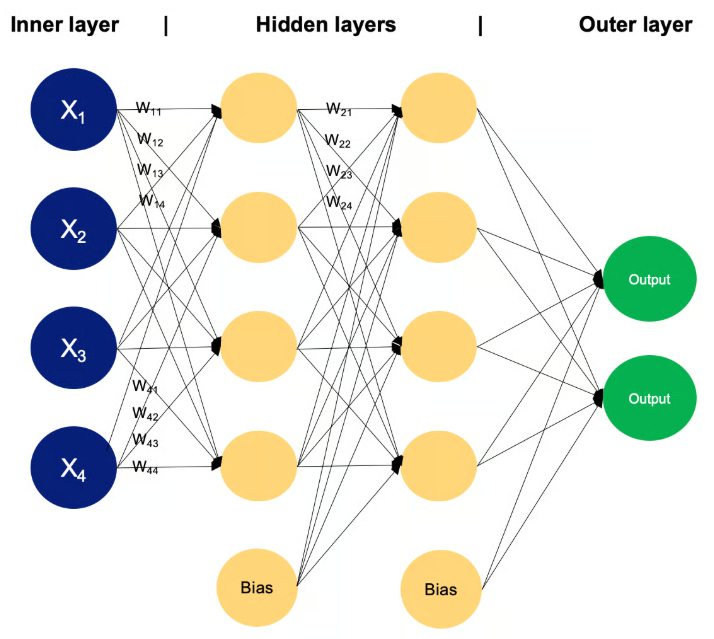
\includegraphics[width=0.8\textwidth]{imagenes/MLP.png}
    \caption{Funcionamiento de un Perceptrón Multicapa según \cite{Perceptrón Multicapa}.}
\end{figure}

El funcionamiento del MLP se basa en un proceso iterativo que combina la propagación de la información hacia adelante, el cálculo del error y la actualización de los parámetros del modelo. En primer lugar, durante la fase de propagación hacia adelante, los datos de entrada se introducen en la red y atraviesan cada una de las capas. En cada neurona se realiza una combinación lineal de las entradas, ponderadas mediante los pesos del modelo y ajustadas por un término de sesgo, según la expresión:

\[
z = \sum w_i x_i + b
,\]

donde \(x_i\) es el valor de la i-ésima variable de entrada, \(w_i\) es el peso asociado a la variable \(x_i\), que determina su influencia en la neurona y \(b\) es el término de sesgo (\emph{bias}), que permite desplazar la función de activación. A continuación, se aplica una función de activación no lineal, que permite transformar la salida y dotar al modelo de la capacidad de aprender relaciones complejas entre las variables. Este proceso se repite de forma sucesiva en cada capa hasta obtener la predicción final del modelo. Una vez generada la predicción, se procede al cálculo del error mediante una función de pérdida, que mide la diferencia entre el valor real y el valor estimado. En el caso de problemas de clasificación binaria, es habitual utilizar la entropía cruzada, que penaliza especialmente las predicciones incorrectas con alta confianza 

\[
L(y, \hat{y}) = - \left( y \log(\hat{y}) + (1 - y)\log(1 - \hat{y}) \right)
,\]

donde \(y\) es el valor real de la variable objetivo e \(\hat{y}\) es el valor predicho por el modelo. El siguiente paso sería concretar cómo afectan los parámetros del modelo a dicho error. Para ello, se utiliza el algoritmo de retropropagación, que permite calcular el gradiente de la función de pérdida respecto a los pesos y sesgos mediante la aplicación de la regla de la cadena

\[
\nabla J(\theta) = \frac{\partial L}{\partial \theta}
,\]

donde \(L\) es la función de pérdida y \(\theta\) es el conjunto de parámetros del modelo, pesos y sesgos. Una vez obtenido el gradiente, los parámetros del modelo se actualizan con el objetivo de minimizar el error. Este ajuste se realiza normalmente mediante el algoritmo de descenso por gradiente, según la expresión:

\[
\theta_{t+1} = \theta_t - \eta \nabla J(\theta_t)
,\]

donde \(\theta_t\) son los parámetros del modelo en la iteración \(t\), \(\theta_{t+1}\): son los parámetros actualizados en la siguiente iteración, \(\eta\) es la tasa de aprendizaje, que controla el tamaño de los ajustes y \(\nabla J(\theta_t)\) el gradiente de la función de pérdida en la iteración \(t\).

Durante el entrenamiento del modelo, se repite de manera iterativa este proceso de difusión, determinación del error y modificación de los parámetros. En la práctica, el entrenamiento no se efectúa en cada iteración con el conjunto de datos entero, sino que se hace con subconjuntos denominados \emph{mini-batches}, los cuales normalmente contienen 1000 datos cada uno. Esta modificación permite que el proceso de aprendizaje sea más estable y que la eficiencia computacional se optimice. MLP puede adecuar de manera gradual sus parámetros para acercarse a funciones complejas y representar relaciones no lineales entre las variables, gracias a este procedimiento. Esta capacidad lo convierte en un método muy importante para problemas en los que los modelos lineales resultan insuficientes, como es el caso de la detección de fraude en datos de consumo eléctrico.


\subsubsection{XGBoost}

Se le conoce como \emph{eXtreme Gradient Boosting} y se aplica en la literatura, incluyendo trabajos como \cite{articulo3}, donde se presenta como un método dentro del análisis de las técnicas existentes. Es un algoritmo de aprendizaje automático supervisado que usa árboles de decisión y aplica una versión mejorada del método \emph{gradient boosting}. El propósito es desarrollar un modelo predictivo sólido mediante la combinación secuencial de varios modelos débiles, que normalmente son árboles de decisión poco profundos. Los modelos no se entrenan de manera independiente; en su lugar, cada nuevo árbol se crea particularmente para rectificar los fallos que cometieron los árboles anteriores. Es reconocido por su rapidez, eficacia y habilidad para escalar eficientemente con conjuntos de datos extensos. El algoritmo opera a través de un proceso iterativo, donde en cada paso se agrega un árbol nuevo que busca acercarse a los residuos o errores del modelo vigente. Estos desechos son la diferencia entre los valores reales y las predicciones hechas hasta ese instante.

La preparación de los datos es el primer paso para poder explicar el algoritmo. Para ello es imprescindible dividir el conjunto de datos en dos grupos menores, uno para entrenar el modelo y otro para comprobar su desempeño. Después, los datos se convierten en el formato \emph{DMatrix}, que es la estructura interna de XGBoost optimizada. Este formato se ha creado con el objetivo de optimizar la velocidad de entrenamiento y el uso de memoria, lo cual es esencial en casos que involucran grandes cantidades de datos. Una vez los datos han sido preparados, se inicia la creación del modelo. Activando el algoritmo y escogiendo una función objetivo apropiada según la clase de problema. El modelo se entrena utilizando el conjunto de entrenamiento y se crean predicciones sobre el conjunto de prueba. La evaluación del modelo se lleva a cabo mediante la comparación de las predicciones con los valores reales, utilizando para ello métricas como la sensibilidad (\emph{recall}), la precisión, la exactitud o la puntuación F1. El empleo de la matriz de confusión permite el análisis más detallado de los fallos y aciertos del modelo.

El proceso de ajuste de hiperparámetros es algo común para optimizar el desempeño del modelo. Este proceso implica hallar la combinación ideal de parámetros para maximizar el potencial predictivo del modelo. La validación cruzada y la búsqueda en cuadrícula son métodos que posibilitan indagar distintas configuraciones de forma sistemática. Uno de los hiperparámetros más importantes es la tasa de aprendizaje, que regula cuánto aporta cada árbol al modelo final. Si este parámetro tiene un valor bajo, el aprendizaje es más lento pero más sólido, lo cual disminuye la probabilidad de sobreajuste. Si el parámetro tiene un valor alto, el aprendizaje se acelera a espera de una posible pérdida de generalización.

\begin{figure}[H]
    \centering
    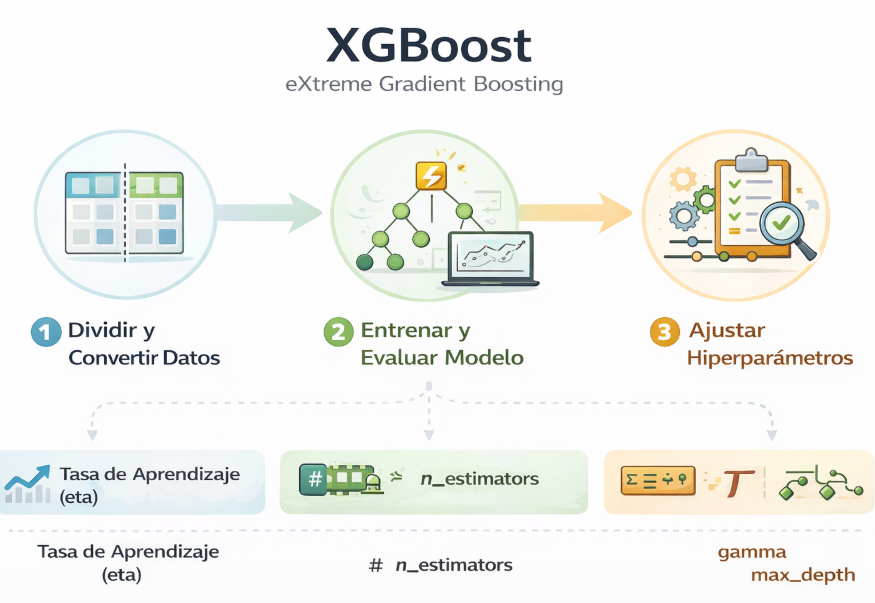
\includegraphics[width=0.8\textwidth]{imagenes/xgboostProceso.png}
    \caption{Funcionamiento XGBoost.}
\end{figure}

La implementación de mecanismos para la regularización, que contribuyen a prevenir el sobreajuste, es una de sus características más importante. Estos procedimientos castigan la complejidad del modelo, lo que restringe el crecimiento desmedido de los árboles y promueve soluciones más universales. Sobre el rendimiento, su diseño permite que sea escalable y de alta eficiencia. Facilita la paralelización en el momento de construir los árboles, lo que disminuye notablemente los tiempos de entrenamiento en comparación con otros métodos de \emph{boosting}. Además, es capaz de manejar amplios volúmenes de datos y optimiza la utilización de memoria, lo cual lo hace muy bueno para implementar aplicaciones en situaciones reales y para resolver problemas a gran escala. Su flexibilidad es otro aspecto que merece ser destacado, pues ayuda al uso de distintas funciones de pérdida según el problema. También, su habilidad para captar conexiones no lineales y gestionar interacciones complejas entre variables lo vuelven particularmente eficaz en situaciones con datos tabulares o estructurados.

Sin embargo, este método también presenta ciertas limitaciones. Su correcto funcionamiento depende en gran medida del ajuste de hiperparámetros, lo que puede requerir un proceso de optimización complejo. Además, sigue siendo menos transparente que modelos más simples. Por último, su complejidad computacional, aunque optimizada, puede ser elevada en comparación con algoritmos más básicos. Para terminar, XGBoost representa una evolución avanzada del \emph{gradient boosting} que combina precisión, eficiencia y robustez. Gracias a sus mejoras en optimización, regularización y escalabilidad, se convierte en uno de los algoritmos más utilizados en el ámbito del aprendizaje automático, especialmente en problemas donde se requiere un alto rendimiento predictivo.


\subsection{Técnicas \emph{online}}

Los algoritmos de aprendizaje automático \emph{online} permiten la actualización paulatina de sus parámetros conforme se van recibiendo nuevas instancias de datos, sin requerir que el modelo entero sea reentrenado desde el principio. Es especialmente bueno, cuando los datos fluyen de manera continua, como en sistemas reales que monitorean el consumo eléctrico. En estas situaciones, los modelos tienen que ser capaces de ajustarse a las alteraciones en los patrones de consumo; este fenómeno se llama \emph{concept drift} o deriva de concepto. En él, la distribución de los datos cambia con el tiempo. Por eso, la detección de fraude eléctrico en tiempo real es considerada como esencial para el aprendizaje online. La selección de técnicas \emph{online} se realiza en base a su presencia en la literatura científica sobre la detección de fraude eléctrico en flujos de datos. En este proyecto se seleccionan algoritmos representativos de distintos modos, incluyendo un modelo \emph{baseline} que permita establecer un punto de referencia.


\subsubsection{Perceptrón}

El perceptrón es uno de los algoritmos más básicos del aprendizaje supervisado \emph{online} y constituye un clasificador lineal que actualiza sus pesos únicamente cuando comete errores de clasificación. Se selecciona este modelo como baseline, debido a su simplicidad, bajo coste computacional y capacidad de aprendizaje incremental puro. Además, se utilizará para comparar el rendimiento de técnicas más complejas.

Es un modelo de clasificación binaria que aprende a partir de los datos mediante un proceso iterativo de ajuste de pesos. Su funcionamiento se basa en la combinación lineal de las variables de entrada y una función de activación que determina la clase predicha. Dado un vector de entrada \( x = (x_1, x_2, ..., x_n) \) y un vector de pesos asociado \( w = (w_1, w_2, ..., w_n) \), el modelo calcula en primer lugar una combinación lineal de las variables:

\[z = \mathbf{w} \cdot \mathbf{x} + b ,\]

donde \( b \) es el término de sesgo o \emph{bias}. A continuación, se aplica una función de activación que transforma el valor obtenido en una salida binaria:

\[
f(x) =
\begin{cases}
1 & \text{si } z > 0 \\
0 & \text{en otro caso}
\end{cases}
.\]

Esta salida representa la clase predicha por el modelo para la instancia de entrada. El proceso de aprendizaje del perceptrón se basa en la corrección de errores. Para cada nueva instancia, el modelo realiza una predicción \( \hat{y} \), que se compara con la etiqueta real \( y \). A partir de esta comparación se calcula el error:

\[
error = y - \hat{y}
,\]

Si la predicción es correcta, los pesos no se modifican. Sin embargo, si existe un error, el modelo actualiza sus parámetros para mejorar futuras predicciones. La actualización de los pesos se realiza mediante la siguiente regla:

\[
\mathbf{w} = \mathbf{w} + \eta \cdot error \cdot \mathbf{x}
,\]

\[
b = b + \eta \cdot error
,\]

donde \( \eta \) es la tasa de aprendizaje, que controla la magnitud del ajuste.

\begin{figure}[H]
    \centering
    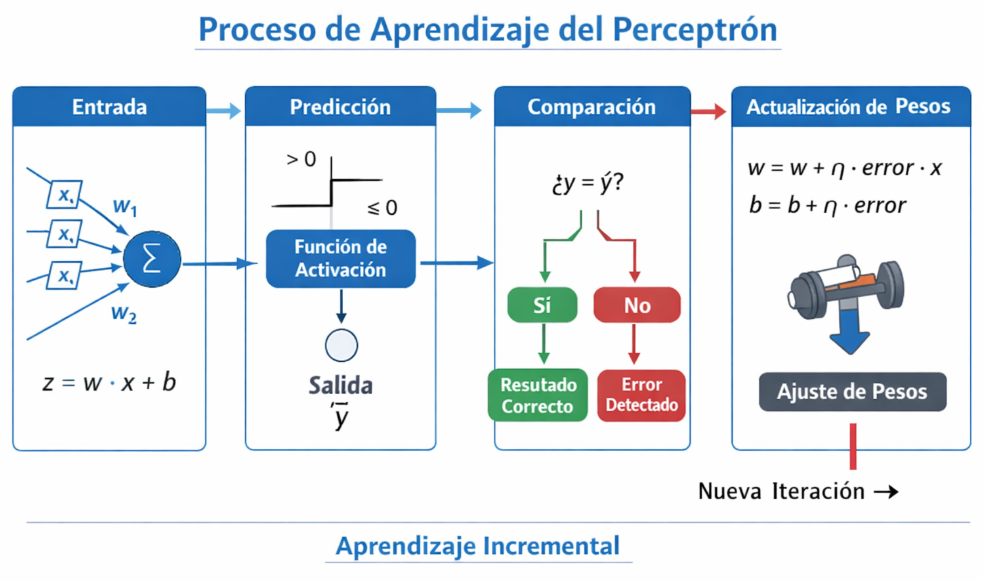
\includegraphics[width=0.8\textwidth]{imagenes/Perceptron.png}
    \caption{Proceso de aprendizaje del Perceptrón.}
\end{figure}

Este proceso se repite de forma secuencial para cada nueva instancia de datos, siguiendo un esquema de aprendizaje incremental en el que el modelo predice, evalúa el error y actualiza sus parámetros en tiempo real. Gracias a este mecanismo, este modelo es capaz de adaptarse progresivamente a los patrones de los datos, lo que lo convierte en un algoritmo adecuado para entornos de aprendizaje online. Sin embargo, al tratarse de un modelo lineal, su capacidad para tratar relaciones complejas entre variables es bastante limitada.


\subsubsection{Naive Bayes incremental}

El modelo Naive Bayes es un clasificador probabilístico basado en la regla de Bayes, que asume independencia condicional entre las variables de entrada. Esto significa que cada característica contribuye de forma independiente a la probabilidad final de pertenencia a una clase. Este método es utilizado en la literatura sobre detección de fraude eléctrico en trabajos como \cite{articulo1}, debido a su eficiencia y buen rendimiento en escenarios de clasificación en tiempo real. A partir del teorema de Bayes, la probabilidad de una clase \( y \) dado un vector de entrada \( x \) se calcula como:

\[
P(y|x) = \frac{P(x|y)\,P(y)}{P(x)}
,\]

donde \( y \) es la clase donde se encuentra un ejemplo de entrenamiento o dato y \( x \) las características de un ejemplo o dato para saber si pertenecen a una clase. Dado que \( P(x) \) es constante para todas las clases, la predicción se realiza maximizando

\[
P(y|x) \propto P(y) \prod_{i=1}^{n} P(x_i | y)
,\]

donde \( P(y) \) es la probabilidad a priori de la clase y \( P(x_i | y) \) es la probabilidad condicional de cada característica dada la clase, es decir, la probabilidad de los datos de presentar las características \( x \) cuando pertenecen a la clase \( y \). El modelo clasifica una nueva instancia asignándole la clase con mayor probabilidad posterior.

En su versión incremental, \emph{online}, Naive Bayes no requiere almacenar todos los datos ni reentrenarse desde cero. En su lugar, mantiene estimaciones acumuladas de las probabilidades y las actualiza conforme llegan nuevas observaciones. Para cada nueva instancia, se calcula la predicción utilizando las probabilidades actuales. Despúes, se compara con la etiqueta real y se actualizan las probabilidades. La probabilidad a priori \( P(y) \), mediante el recuento de clases y las probabilidades condicionales \( P(x_i | y) \), actualizando estadísticas como medias, varianzas o frecuencias.

\begin{figure}[H]
    \centering
    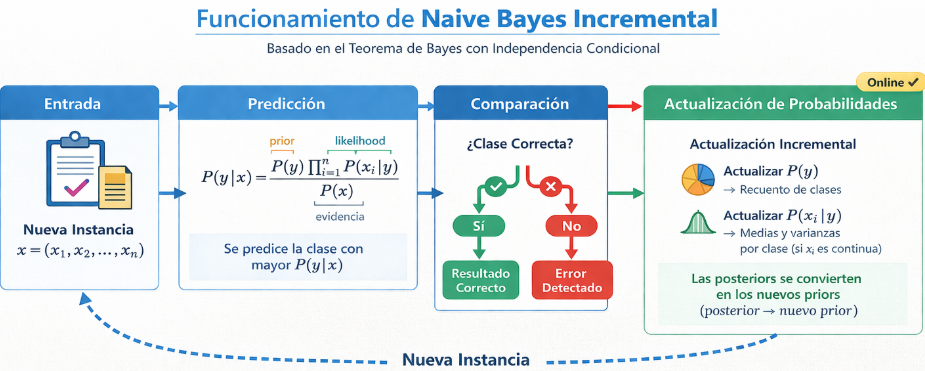
\includegraphics[width=0.95\textwidth]{imagenes/naive.png}
    \caption{Funcionamiento de Naive Bayes incremental.}
\end{figure}

La principal diferencia respecto a la versión \emph{offline} es que el modelo clásico estima todas las probabilidades utilizando el conjunto completo de entrenamiento de una sola vez, mientras que el modelo incremental actualiza estas estimaciones de forma continua sin necesidad de acceder a los datos históricos completos. Esto lo hace especialmente adecuado para escenarios de flujo de datos donde la información llega de manera secuencial. Este método presenta ventajas importantes en entornos \emph{online}, como su bajo coste computacional, su rapidez de actualización y su estabilidad ante grandes volúmenes de datos.


\subsubsection{K Vecinos más cercanos \emph{online}}

El algoritmo k vecinos más cercanos (kNN) es un método basado en instancias que clasifica una nueva observación en función de la clase mayoritaria de sus vecinos más cercanos en el espacio de características. Su funcionamiento general, así como las distintas métricas de distancia, la influencia del parámetro $k$ y sus referencias en la literatura, han sido descritos previamente en la sección de técnicas offline.

En su versión \emph{online}, el funcionamiento del algoritmo se mantiene prácticamente igual, pero introduce cambios en la gestión del conjunto de datos. En lugar de trabajar con un conjunto de entrenamiento estático, el modelo añade progresivamente nuevas instancias a medida que estas llegan en forma de flujo de datos. De este modo, el conjunto de referencia utilizado para calcular los vecinos más cercanos se va actualizando continuamente, permitiendo al modelo adaptarse a posibles cambios en los patrones de consumo eléctrico. La predicción sigue basándose en el cálculo de distancias entre la nueva instancia y las observaciones almacenadas, siendo la distancia euclídea una de las más utilizadas

\[
d(x_i, x_j) = \sqrt{\sum (x_i - x_j)^2}
.\]

Sin embargo, esta adaptación al entorno online se encuentra con algunos retos. A medida que el número de instancias almacenadas crece, el coste computacional aumenta significativamente, lo que puede afectar a la eficiencia del modelo en tiempo real. Por este motivo, en implementaciones prácticas se suelen emplear estrategias adicionales, como ventanas deslizantes o técnicas de olvido, que permiten limitar el tamaño del conjunto de datos y priorizar la información más reciente.

\begin{figure}[H]
    \centering
    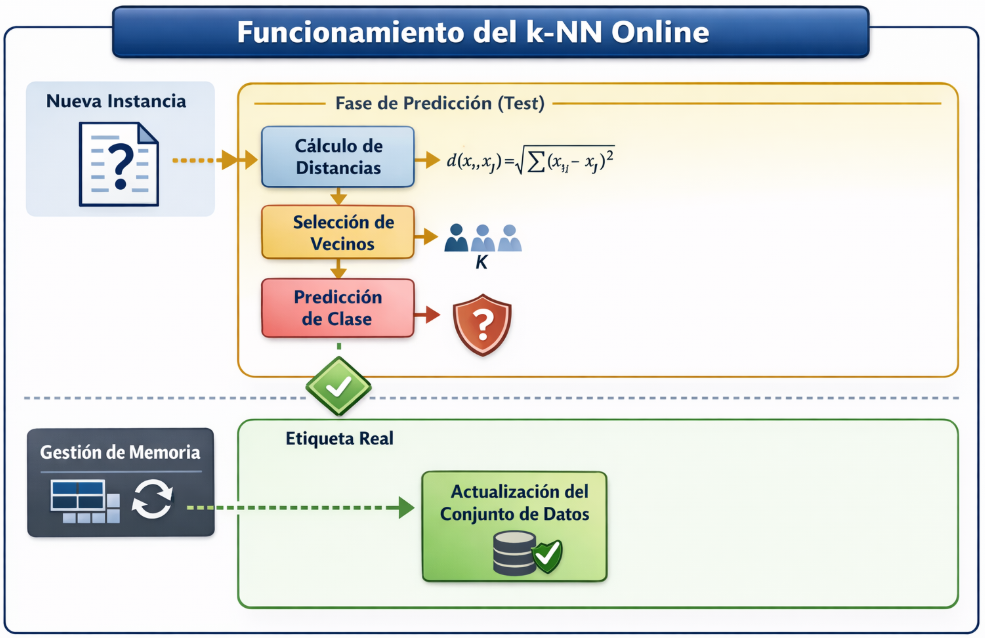
\includegraphics[width=0.8\textwidth]{imagenes/knnOnline.png}
    \caption{Funcionamiento del kNN online.}
\end{figure}

La técnica de ventanas deslizantes consiste en mantener únicamente un subconjunto reciente de los datos, eliminando las instancias más antiguas a medida que llegan nuevas observaciones, lo que permite al modelo centrarse en los patrones más actuales. Por otro lado, la técnica de olvido se basa en asignar menor peso a las instancias antiguas en el proceso de aprendizaje, reduciendo progresivamente su influencia sin necesidad de eliminarlas completamente. Su inclusión en este trabajo permite comparar el comportamiento de modelos basados en proximidad tanto en entornos \emph{offline} como \emph{online}, analizando su capacidad de adaptación frente a cambios en los datos.


\subsubsection{\emph{Hoeffding Tree}}

El \emph{Hoeffding Tree}, también conocido como \emph{Very Fast Decision Tree} (VFDT), es un algoritmo diseñado específicamente para el aprendizaje en flujos de datos, donde las observaciones llegan de manera continua y no es posible almacenar todo el conjunto de datos. Este algoritmo es utilizado en la literatura de detección de fraude eléctrico en trabajos como \cite{articulo1} y \cite{articulo4}, destacando por su capacidad para procesar grandes volúmenes de información en tiempo real y adaptarse a cambios en los patrones de consumo. A diferencia de los árboles de decisión tradicionales en entornos \emph{offline}, este modelo construye el árbol de forma incremental, procesando cada instancia una única vez y actualizando sus estadísticas internas sin necesidad de reentrenamiento.

El funcionamiento del algoritmo se basa en el uso del límite de Hoeffding, que permite tomar decisiones de partición con garantías estadísticas utilizando únicamente un subconjunto de los datos. Este límite establece que, con un número suficiente de observaciones, la media estimada de una variable converge a su valor real con alta probabilidad. Formalmente, el límite de Hoeffding se define como:

\[
\epsilon = \sqrt{\frac{R^2 \ln(1/\delta)}{2n}}
,\]

donde $R$ es el rango de la variable, $\delta$ es la probabilidad de error y $n$ es el número de observaciones. Este límite se utiliza para determinar cuándo existe suficiente evidencia estadística para dividir un nodo. Para ello, el algoritmo evalúa distintas características mediante una función de mérito y selecciona las dos mejores. Si la diferencia entre ambas supera el umbral $\epsilon$, se realiza la división del nodo con la mejor característica.

\begin{figure}[H]
    \centering
    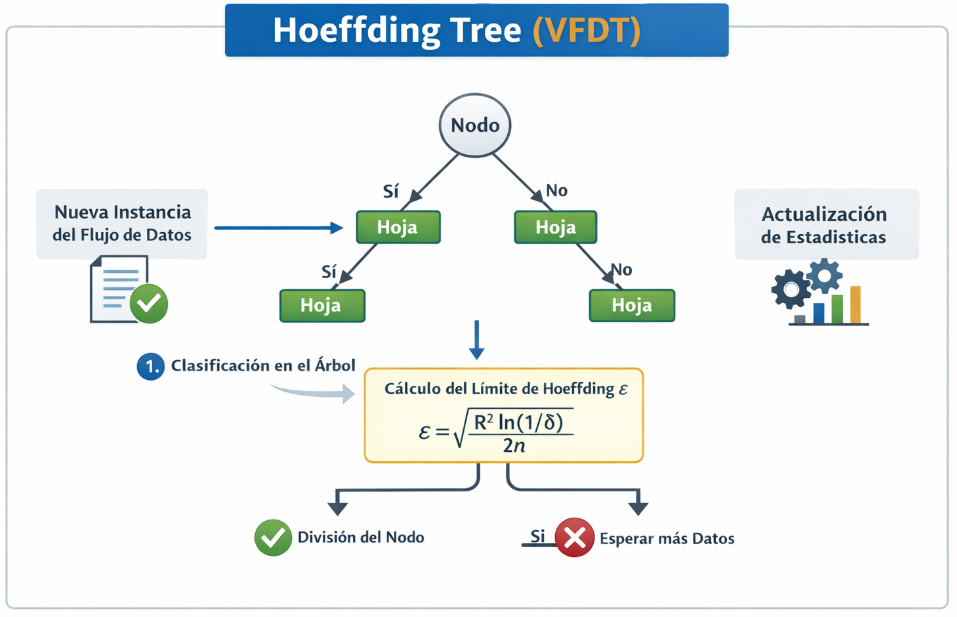
\includegraphics[width=0.87\textwidth]{imagenes/hoeffding.png}
    \caption{Funcionamiento del Hoeffding Tree.}
\end{figure}

Su proceso de funcionamiento puede resumirse de la siguiente forma. Para empezar, se recibe una nueva instancia del flujo de datos, esta se clasifica recorriendo el árbol hasta llegar a una hoja. Después, se actualizan las estadísticas de la hoja correspondiente y se comprueba si existen suficientes datos para realizar una división utilizando el límite de Hoeffding. Si se cumple la condición, el nodo se divide generando nuevas ramas. Este proceso permite construir árboles de decisión de manera eficiente y escalable, siendo capaz de aproximar el comportamiento de un árbol entrenado con un conjunto de datos completo, pero con un coste computacional mucho menor.

Para terminar, los \emph{Hoeffding Trees} pueden extenderse para manejar la deriva de concepto mediante mecanismos adicionales como el uso de ventanas deslizantes, lo que los hace especialmente adecuados para entornos dinámicos como la detección de fraude eléctrico.


\subsubsection{\emph{Adaptive Random Forest}}

\emph{Adaptive Random Forest} (ARF) es una extensión del algoritmo \emph{Random Forest} adaptada al aprendizaje \emph{online}, diseñada para trabajar con flujos de datos y entornos dinámicos donde la distribución de los datos puede cambiar con el tiempo. Este algoritmo ha demostrado un rendimiento muy bueno en estudios comparativos de detección de fraude eléctrico en entornos \emph{online} como en el trabajo \cite{articulo1}, debido a su capacidad para combinar múltiples clasificadores y adaptarse a cambios en los patrones de consumo.

El funcionamiento de ARF se basa en la construcción de un conjunto de árboles de decisión incrementales, donde cada árbol se entrena de forma independiente utilizando diferentes subconjuntos de datos y características. Para ello, se emplea una técnica de \emph{online bagging}, en la que cada instancia del flujo de datos se replica un número de veces determinado por una distribución de Poisson, generando así diversidad entre los modelos.

Cada árbol del conjunto es un \emph{Hoeffding Tree} que aprende de forma incremental, cuando llega una nueva instancia, el proceso se desarrolla de la siguiente manera. Para empezar, la instancia se envía a todos los árboles del conjunto, cada árbol realiza una predicción de forma independiente. Después, las predicciones se combinan mediante votación mayoritaria para obtener la predicción final y la instancia se utiliza para actualizar cada árbol según el esquema de aprendizaje incremental.

\begin{figure}[H]
    \centering
    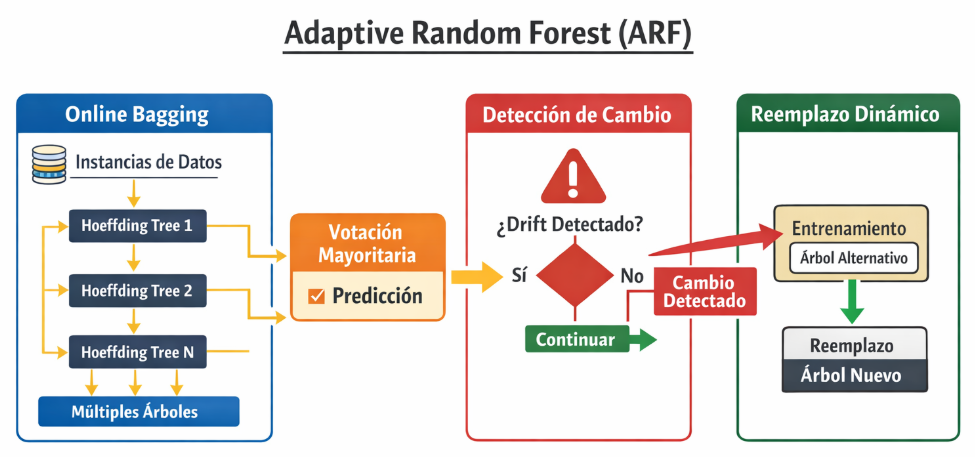
\includegraphics[width=0.8\textwidth]{imagenes/arf.png}
    \caption{Funcionamiento del Adaptive Random Forest.}
\end{figure}

Uno de los aspectos más importantes junto a que combina múltiples \emph{Hoeffding Trees} como clasificadores bases, es su capacidad para adaptarse a la deriva del concepto. Para ello, cada árbol incorpora un detector de cambios que monitoriza el rendimiento del modelo a lo largo del tiempo. Cuando se detecta una degradación significativa en el rendimiento, se activa un mecanismo de adaptación. El mecanismo funciona de la siguiente manera, se entrena un árbol alternativo en segundo plano utilizando los datos recientes. Si el detector confirma un cambio en la distribución de los datos, el árbol original es reemplazado por el árbol alternativo.

Además, ARF introduce diversidad en el conjunto mediante dos mecanismos principales. Uno es el \emph{bagging online}, donde cada árbol recibe una versión ligeramente distinta del flujo de datos. Y el otro, es la selección aleatoria de características, donde cada nodo del árbol se evalúa un subconjunto aleatorio de variables. Estas estrategias permiten mejorar la capacidad de generalización del modelo y reducir el riesgo de sobreajuste.

En comparación con el \emph{Random Forest} tradicional en aprendizaje automático \emph{offline}, ARF presenta varias ventajas clave: permite el aprendizaje \emph{online} sin necesidad de reentrenamiento, es capaz de adaptarse a cambios en los datos en tiempo real y mantiene un alto rendimiento en escenarios dinámicos. Por estas razones, se considera uno de los métodos más avanzados dentro del aprendizaje automático \emph{online} y constituye una referencia clave en este trabajo para evaluar el rendimiento de modelos incrementales en la detección de fraude eléctrico.


% =========================
% CAPÍTULO 5
% =========================
\chapter{Métricas}


\section{Métricas de evaluación}

En la detección de fraude eléctrico, la selección de métricas de evaluación resulta especialmente importante debido al desbalance existente entre las clases y el distinto coste asociado a los errores de clasificación. Por un lado, el conjunto de datos seleccionado presenta una mayor proporción de consumos normales frente a casos de fraude, lo que puede llevar a métricas como la \emph{accuracy} a ofrecer resultados engañosos. Por otro lado, los errores no tienen el mismo impacto: un falso negativo implica no detectar un fraude real, mientras que un falso positivo puede generar costes operativos y molestias a clientes legítimos.

Una métrica es un valor numérico o categórico que permite cuantificar la calidad de las predicciones de un modelo. Su papel es vital durante todas las etapas del desarrollo de un modelo de aprendizaje automático, ya que permite determinar si un modelo cumple con las expectativas. Dependiendo de los resultados obtenidos, las métricas permiten comparar objetivamente varios modelos entre sí, elegir el modelo más efectivo o cambiar los hiperparámetros de un modelo.

En el caso de los modelos \emph{offline}, las métricas se calculan sobre un conjunto de test fijo. Sin embargo, en el aprendizaje \emph{online}, las métricas se evalúan de forma incremental mediante esquemas como la evaluación prequential, donde el modelo es evaluado y actualizado secuencialmente con cada nueva instancia. Esto implica que las métricas reflejan la evolución del rendimiento del modelo a lo largo del tiempo, permitiendo analizar su capacidad de adaptación ante cambios en la distribución de los datos. En este caso estamos antes una métrica de valor categórico porque se tiene un contexto de clasificación, fraude o no. Por este motivo, se seleccionan métricas representativas que permiten evaluar el rendimiento del modelo desde diferentes perspectivas, tanto en escenarios \emph{offline} como en aprendizaje \emph{online}.


\subsection{\emph{Accuracy}}

La \emph{accuracy} o exactitud utilizada en la literatura en trabajos como \cite{articulo1}, \cite{articuloBase}, \cite{articulo2}, \cite{articulo3} y \cite{articulo5}, representa la proporción total de instancias correctamente clasificadas respecto al total de predicciones realizadas. Esta métrica tiene en cuenta tanto los verdaderos positivos como los verdaderos negativos, proporcionando una visión global del rendimiento del modelo. Aunque se utilizará como métrica descriptiva general, no será el criterio principal de comparación debido a la posible influencia del desbalance entre clases.

\[
\text{Accuracy} = \frac{\text{Número de predicciones correctas}}{\text{Número total de predicciones}}
.\]

El valor de esta métrica se encuentra entre 0 y 1, donde valores cercanos a 1 indican un mejor rendimiento del modelo. Como se destacó antes, hay que tener en cuenta que evalúa mal el rendimiento de un modelo basado en datos desequilibrados, o datos en los que los errores de predicción no tienen el mismo impacto. Por ello, el resto de métricas que se verán a continuación para ayudar a realizar una evaluación correcta.


\subsection{\emph{Precision}}

La precisión utilizada en la literatura en trabajos como \cite{articulo1}, \cite{articuloBase}, \cite{articulo2} y \cite{articulo5}, mide la proporción de instancias clasificadas como fraude que realmente corresponden a fraude. Esta métrica permite evaluar el número de falsos positivos generados por el modelo, aspecto esencial para evitar clasificaciones incorrectas de clientes sin comportamiento posible de fraude. Su fórmula es

\[
\text{Precision} = \frac{TP}{TP + FP}
,\]

donde $TP$ representa el número de verdaderos positivos y $FP$ representa el número de falsos positivos. A diferencia de la \emph{accuracy} o exactitud, esta métrica se centra únicamente en las predicciones positivas, siendo especialmente relevante en escenarios donde el coste de los falsos positivos es elevado, como en la detección de fraude eléctrico.


\subsection{\emph{Recall}}

El \emph{recall} o también conocido en español como exhaustividad, sensibilidad o tasa de verdaderos positivos mide la proporción de fraudes reales correctamente detectados por el modelo. Esta métrica se utiliza en la literatura en trabajos como \cite{articulo1}, \cite{articulo2} y \cite{articulo5}. En la detección de fraude eléctrico, esta métrica resulta ser igual que otra métrica de fraudes llamada Tasa de Detección (DR) utilizada en la literatura en trabajos como \cite{articuloBase}.

\[
\text{Recall} = \frac{TP}{TP + FN}
,\]

donde $TP$ representa el número de verdaderos positivos y $FN$ representa el número de falsos negativos. Esta métrica es útil cuando el costo de los falsos negativos es alto. Además, su elección es realmente importante en este trabajo y en la literatura, ya que los falsos negativos implican no detectar casos reales de fraude. Estos falsos negativos pueden llevar a pérdidas millonarias para las empresas eléctricas.


\subsection{\emph{F1-score}}

La puntuación F1 utilizada en la literatura en trabajos como \cite{articulo1}, \cite{articuloBase}, \cite{articulo2} y \cite{articulo5}, es la media armónica entre la precisión y el \emph{recall}, proporcionando una medida equilibrada del rendimiento del modelo cuando existe desbalance de clases, como es este caso. En este estudio, el \emph{F1-score} se considerará una de las métricas principales para la comparación entre técnicas.

Entrando más en detalle, esta métrica equilibra la compensación entre falsos positivos y falsos negativos, y proporciona una medida más precisa del rendimiento del modelo. En la detección de fraude, la precisión por sí sola no es suficiente para comprender la situación completa. Un modelo puede alcanzar una alta precisión, pero si no detecta casos críticos poco frecuentes, podría estar causando más fallos que beneficios. Con esta métrica se estará cubriendo este riesgo. Se define como:

\[
F_1 = 2 \cdot \frac{\text{Precision} \cdot \text{Recall}}{\text{Precision} + \text{Recall}}
,\]

siendo \emph{Precision}, la fórmula de la métrica de \emph{Precision}, y \emph{Recall}, la fórmula de la métrica de \emph{Recall} antes vistas. Se utiliza la media armónica en vez de la media aritmética porque esta última penaliza las grandes diferencias. En caso de alta precisión pero baja recuperación (o viceversa), el f1-score disminuirá significativamente, lo que refleja un desequilibrio.


\subsection{\emph{False Positive Rate}}

La Tasa de Falsos Positivos (FPR) utilizada en la literatura en trabajos como \cite{articuloBase}, mide la proporción de instancias normales que han sido incorrectamente clasificadas como fraude. Se define como:

\[
FPR = \frac{FP}{FP + TN}
,\]

donde $FP$ (Falsos Positivos) es el número de instancias normales clasificadas erróneamente como fraude, $TN$ (Verdaderos Negativos) es el número de instancias normales correctamente clasificadas y el denominador $(FP + TN)$ representa el total de usuarios legítimos, por lo que el FPR indica qué fracción de estos usuarios está siendo incorrectamente señalada como fraudulenta.

Esta métrica resulta especialmente relevante en la detección de fraude eléctrico, ya que un alto número de falsos positivos puede implicar costes adicionales derivados de inspecciones innecesarias o afectar negativamente a la experiencia de clientes legítimos. Por este motivo, el FPR se utiliza en la literatura como una medida complementaria al \emph{recall}, permitiendo evaluar el equilibrio entre detección de fraude y tasa de falsas alarmas.


\subsection{ROC-AUC}

El área bajo la curva ROC es una métrica utilizada en problemas de clasificación desbalanceados y en la literatura sobre detección de fraude eléctrico en trabajos como \cite{articuloBase} y \cite{articulo3}, ya que evalúa la capacidad de un modelo para distinguir entre clases a lo largo de distintos umbrales de decisión.

La curva ROC representa gráficamente la relación entre la tasa de verdaderos positivos (TPR) y la tasa de falsos positivos (FPR), para todos los posibles valores del umbral de clasificación. Estas tasas se definen como:

\[
TPR = \frac{TP}{TP + FN}, \quad FPR = \frac{FP}{FP + TN}
,\]

donde $TP$ (Verdaderos Positivos) representa los fraudes correctamente detectados, $FN$ (Falsos Negativos) los fraudes no detectados, $FP$ (Falsos Positivos) los usuarios normales clasificados como fraude y $TN$ (Verdaderos Negativos) los usuarios normales correctamente clasificados.

La curva ROC se construye variando el umbral de decisión del modelo, por ejemplo en este trabajo podría ser el valor a partir del cual se considera fraude. Para cada umbral se obtiene un par $(FPR, TPR)$, generando así la curva completa. El área bajo esta curva (AUC) es un valor escalar entre 0 y 1 que resume el rendimiento global del modelo siendo $AUC = 1$ una clasificación perfecta, $AUC \approx 0.5$ un comportamiento aleatorio y $AUC < 0.5$ peor que el azar. Una interpretación especialmente importante es que el AUC representa la probabilidad de que el modelo asigne una mayor puntuación a una instancia positiva, fraude, que a una negativa, consumo normal.

A diferencia de métricas como \emph{accuracy}, \emph{precision} o \emph{recall}, esta es independiente de un umbral concreto, ya que evalúa el comportamiento del modelo en todos los posibles puntos de operación . Esto lo convierte en una métrica especialmente útil en problemas con clases desbalanceadas, como la detección de fraude eléctrico. Además, permite analizar el compromiso entre detectar el mayor número de fraudes posibles, alto TPR, y minimizar falsas alarmas, bajo FPR. Por todas estas razones y motivos, considero a esta métrica una buena forma de evaluar los resultados de los métodos de aprendizaje automáticos de este trabajo.


\subsection{Matriz de confusión}

Es una métrica para la visualización de los resultados de algoritmos clasificadores. Es una tabla que desglosa el número de instancias de verdad fundamental de una clase específica frente al número de instancias de clase previstas. Las matrices de confusión son una de las diferentes métricas de evaluación que miden el rendimiento de un modelo de clasificación.

Destacar que ninguno de los artículos analizados presenta explícitamente la matriz de confusión, pero todos utilizan métricas que derivan directamente de ella, excepto el artículo \cite{articulo4}, por lo que su uso es implícito en todos los trabajos estudiados. Además, esta métrica permite analizar detalladamente los aciertos y errores del modelo, distinguiendo entre verdaderos positivos, falsos positivos, verdaderos negativos y falsos negativos. Una de sus principales ventajas es que pueden utilizarse con cualquier algoritmo clasificador, como Naïve Bayes, modelos de regresión, árboles de decisión, etc, modelos que serán implementados. 

En la práctica, debido a su amplia aplicabilidad en la ciencia de datos y en los modelos de aprendizaje automático, muchos paquetes y bibliotecas vienen precargados con funciones para crear matrices de confusión en Python. Su análisis resulta fundamental para interpretar el comportamiento del sistema en la detección de fraude.


\subsection{Coeficiente Kappa}

El coeficiente Kappa es una métrica estadística utilizada en aprendizaje automático en trabajos como \cite{articulo1} para evaluar el rendimiento de un modelo de clasificación. Cuantifica la concordancia entre dos clasificadores en etiquetas categóricas, corrigiendo la concordancia que podría producirse por casualidad. Es decir, mide el grado de concordancia entre las predicciones del modelo y las etiquetas reales, teniendo en cuenta el acuerdo esperado por azar. 

Una de sus principales ventajas es que aporta una evaluación más robusta en escenarios con clases desbalanceadas. Cuando los datos están desbalanceados, la precisión general puede volverse engañosa porque un modelo puede ser muy preciso simplemente al predecir la clase mayoritaria. Esta métrica puede ayudar ajustando el acuerdo que podría ocurrir simplemente debido a la clase mayoritaria, proporcionando una estimación más realista del desempeño del modelo. Se define como:

\[
\kappa = \frac{p_o - p_e}{1 - p_e}
,\]

donde $\mathbf{p_o}$ es la proporción de acuerdo observado (fórmula de la \emph{Accuracy}) y $\mathbf{p_e}$ es la proporción de acuerdo esperado por azar. $\mathbf{p_e}$ se calcula utilizando las probabilidades marginales de cada clase. En clasificación binaria se tiene:

\[
p_e =
P_{\text{real positivo}} \cdot P_{\text{predicho positivo}}
+
P_{\text{real negativo}} \cdot P_{\text{predicho negativo}}
.\]

Es decir, es la probabilidad de coincidir en fraude por azar y más probabilidad de coincidir en normal por azar. Para terminar, el valor kappa de Cohen tiene que tener un rango de entre -1 y 1. Cuanto más cerca de 1, mejor. Es decir, cuando $\kappa \approx 0$ indica que el modelo no presenta capacidad predictiva, si $\kappa > 0.6$ indica un buen rendimiento y si $\kappa > 0.8$ indica un rendimiento excelente.


% =========================
% CAPÍTULO 6
% =========================
\chapter{Experimentación}


\section{Implementación y Configuración de los Modelos}

En esta sección se explica y detalla de una manera clara y completa la implementación de todos los métodos de aprendizaje automático seleccionados anteriormente.


\subsection{Modelos Offline}

Todos los modelos offline implementados en este proyecto siguen un proceso común de preparación de datos, entrenamiento y evaluación. Este procedimiento permite garantizar que los distintos algoritmos se comparen bajo las mismas condiciones experimentales.

En primer lugar, se realiza la carga del conjunto de datos de consumo eléctrico desde el archivo ``df.csv''. Posteriormente, se lleva a cabo un proceso de preprocesamiento de los datos para preparar las variables que serán utilizadas por los modelos de aprendizaje automático. Destaca la variable \emph{theft}, que indica si existe consumo normal o fraude. Esta variable se transforma en una variable binaria, donde el valor 0 representa consumo normal y el valor 1 indica fraude. Además, las variables categóricas presentes en el conjunto de datos se convierten en variables numéricas mediante la técnica de one-hot encoding.

Una vez preparado el conjunto de datos y separadas las variables independientes de la variable objetivo, el conjunto de datos se divide en dos subconjuntos. El conjunto de entrenamiento (80\%), utilizado para entrenar los modelos y el conjunto de pruebas (20\%), utilizado para evaluar su rendimiento. Para asegurar que ambas particiones mantengan la misma proporción de casos de fraude y consumo normal, se utiliza el parámetro \emph{stratify}.

Para garantizar la reproducibilidad de los experimentos, se añade el parámetro \emph{random\_state=42} en la partición de los datos. Este parámetro controla la semilla del generador de números aleatorios, asegurando que la división del conjunto de datos en entrenamiento y prueba sea siempre la misma en diferentes ejecuciones del código. De esta forma, se garantiza que los resultados obtenidos sean comparables y replicables.

Para evaluar la capacidad de generalización del modelo y reducir la varianza asociada a una única partición de los datos, se emplea validación cruzada estratificada con 5 particiones (\emph{Stratified K-Fold}). En este proceso, el conjunto de datos se divide en cinco subconjuntos, garantizando que cada uno de ellos mantiene la misma proporción de clases que el conjunto original, lo cual resulta especialmente importante en problemas con desbalance de clases como la detección de fraude eléctrico. De forma iterativa, se utilizan cuatro particiones para el entrenamiento y una para la validación, repitiendo el proceso hasta completar las cinco combinaciones posibles. Durante la validación cruzada se utiliza la métrica \emph{F1-score}, debido a su precisión y rendimiento en datos desbalanceados, donde es necesario equilibrar la precisión y la capacidad de detección de la clase minoritaria.


\subsubsection{Regresión Logística}

La regresión logística es uno de los algoritmos más utilizados para problemas de clasificación binaria. En este trabajo, se utiliza como modelo \emph{baseline}, es decir, como una referencia simple y rápida de implementar que permite establecer un punto de comparación frente a modelos más complejos.

Para mejorar el rendimiento del algoritmo se utiliza un pipeline que permite aplicar distintas etapas de procesamiento de forma secuencial. En el pipeline se emplea \emph{StandardScaler}, técnica de normalización de datos, para normalizar las variables de entrada, ya que modelos como la regresión logística son sensibles a la escala de los datos. Esta normalización permite mejorar la convergencia del algoritmo y evitar que variables con mayor magnitud dominen el proceso de aprendizaje. Luego, para compensar el desequilibrio existente entre los casos de fraude y consumo normal se utiliza el parámetro \emph{class\_weight = "balanced``}. Una vez definido el pipeline, se realiza la validación cruzada y el modelo se entrena utilizando el conjunto de datos de entrenamiento.

Para terminar, se almacenan los resultados de las métricas calculadas como en todos los métodos anteriores y próximos. A pesar de ser un modelo relativamente simple, la regresión logística permite establecer una primera referencia de rendimiento que posteriormente será comparada con modelos más complejos.


\subsubsection{Random Forest}

Con el objetivo de mejorar el rendimiento obtenido la Regresión logística, se implementa el algoritmo Bosque Aleatorio, uno de los métodos de aprendizaje supervisado más utilizados en problemas de clasificación. Es un algoritmo basado en conjuntos de árboles de decisión. En lugar de construir un único árbol, el algoritmo genera múltiples árboles utilizando diferentes subconjuntos de datos y variables. Posteriormente, cada árbol realiza una predicción y el resultado final se obtiene mediante votación mayoritaria.

Los parámetros principales, para la construcción del modelo, que incluye la configuración son: \emph{n\_estimators} = 200, que indica el número de árboles que forman el bosque, \emph{max\_depth} = 10, que limita la profundidad de los árboles para evitar sobreajuste, \emph{min\_samples\_split} = 5, que es el número mínimo de muestras necesarias para dividir un nodo, \emph{min\_samples\_leaf} = 2, que es el número mínimo de muestras en una hoja, \emph{random\_state} = 42, que es utilizado para garantizar la reproducibilidad de los experimentos, \emph{class\_weight} = "balanced", que ajusta automáticamente el peso de cada clase para compensar el desequilibrio existente en el conjunto de datos y \emph{n\_jobs} = -1, que permite utilizar todos los núcleos disponibles del procesador para acelerar el entrenamiento. Después, se emplea la validación cruzada estratificada, de especial importancia como se comentó anteriormente.

Una de las ventajas principales de este método es que permite estimar la importancia de cada variable en el proceso de clasificación, conocida como \emph{Feature Importance}. Esta medida indica cuánto contribuye cada variable del conjunto de datos a mejorar las decisiones de los árboles que componen el modelo. Cuanto mayor es el valor de importancia de una variable, mayor es su influencia en las predicciones del modelo. Las medidas de importancia de variables obtenidas mediante este modelo pueden presentar cierto sesgo hacia variables con mayor número de categorías o mayor variabilidad, ya que estas tienden a generar más divisiones en los árboles. Por ello, estos resultados deben interpretarse con mucho cuidado y no tomarlos como rigurosos.

Posteriormente, las variables se ordenan según su importancia y se genera un gráfico con las diez variables más relevantes, lo que permite interpretar qué factores tienen mayor influencia en la detección de fraude en el consumo eléctrico. Para terminar, al igual que en el resto de modelos, las métricas de evaluación se almacenan para su posterior comparación.


\subsubsection{Gradient Boosting}

Este método pertenece a la familia de algoritmos de los ensamble, los cuales combinan múltiples modelos débiles, generalmente árboles de decisión poco profundos, para construir un modelo más robusto y preciso. A diferencia de modelos como Bosque Aleatorio, donde los árboles de decisión se entrenan de forma independiente, este modelo construye los árboles de manera secuencial. Cada nuevo árbol se entrena sobre los errores, residuos, cometidos por los modelos anteriores, ajustándose progresivamente a los ejemplos mal clasificados.

Los parámetros principales, para la construcción del modelo, que incluye la configuración son: \emph{n\_estimators} = 200, que es el número de árboles que forman el modelo, \emph{learning\_rate} = 0.1, que controla la contribución de cada árbol al modelo final, \emph{max\_depth} = 3, que es la profundidad máxima de cada árbol y \emph{random\_state} = 42, que es el valor utilizado para garantizar la reproducibilidad de los experimentos. De forma similar a los modelos anteriores, para validar este modelo se aplica validación cruzada estratificada con 5 particiones.

Una vez definido el modelo, se realiza su entrenamiento utilizando el conjunto de datos de entrenamiento. En este entrenamiento hay que destacar, que dado que el algoritmo no permite especificar pesos de clase de forma directa, se emplea la técnica de ponderación de instancias mediante \emph{sample\_weight}, asignando mayor peso a la clase minoritaria durante el entrenamiento, en este caso a fraude.  Este proceso permite mitigar el efecto del desbalance de clases de manera similar al uso de \emph{class\_weight} en otros modelos. El balanceo se aplica únicamente durante el entrenamiento final mediante pesos por instancia, mientras que en la validación cruzada se evalúa el modelo sin ajuste de pesos.

Tras el entrenamiento, se realizan predicciones sobre el conjunto de prueba y se calculan diferentes métricas seleccionadas de evaluación que permiten analizar el rendimiento del modelo. Además, se calcula la importancia de las variables utilizadas por el modelo como en el modelo anterior. En el caso de este modelo, la importancia de cada variable se calcula a partir de la reducción del error que produce cada característica al dividir los nodos de los árboles de decisión. Cuanto mayor sea esta reducción, mayor será la relevancia de la variable en el modelo.

Las variables más importantes se almacenan en un archivo independiente y también se representan mediante un gráfico que muestra las características con mayor influencia en la detección de fraude. Sin embargo, estas medidas pueden presentar cierto sesgo hacia variables con mayor variabilidad o número de posibles divisiones, por lo que deben interpretarse con cautela. Finalmente, las métricas obtenidas se almacenan, permitiendo realizar un análisis comparativo del rendimiento entre los distintos modelos implementados.


\subsubsection{Perceptrón Multicapa}

El Perceptrón Multicapa, MLP, es un modelo de red neuronal artificial compuesto por varias capas de neuronas completamente conectadas. Es capaz de modelar relaciones no lineales entre las variables de entrada gracias al uso de capas ocultas y funciones de activación no lineales. Esta capacidad lo convierte en una alternativa importante para problemas complejos de clasificación como la detección de fraude eléctrico. El modelo se implementa integrándose dentro de un \emph{Pipeline} junto con una etapa previa de escalado. Este escalado resulta necesario, ya que el entrenamiento de las redes neuronales depende en gran medida de que las variables de entrada se encuentren en rangos comparables, favoreciendo un proceso más estable del algoritmo de optimización.

Los parámetros principales, para la construcción del modelo, que incluye la configuración son: \emph{hidden\_layer\_sizes = (100, 50)}, que define una arquitectura con dos capas ocultas de 100 y 50 neuronas, respectivamente; \emph{activation = "relu"}, que establece la función de activación utilizada en las capas ocultas, \emph{solver = "adam"}, que indica el algoritmo de optimización empleado durante el entrenamiento, \emph{alpha = 0.0001}, que introduce regularización para reducir el riesgo de sobreajuste, \emph{batch\_size = 256}, que determina el número de muestras procesadas antes de cada actualización de los pesos, \emph{learning\_rate\_init = 0.001}, que fija la tasa de aprendizaje inicial, \emph{max\_iter = 300}, que marca el número máximo de iteraciones y \emph{random\_state = 42}, utilizado para garantizar la reproducibilidad de los experimentos. Además, se activa \emph{early\_stopping = True}, reservando automáticamente una fracción del conjunto de entrenamiento para validación interna mediante \emph{validation\_fraction = 0.1}. El entrenamiento se detiene cuando no se observan mejoras durante un número determinado de iteraciones consecutivas, fijado mediante \emph{n\_iter\_no\_change = 10}. Este mecanismo permite reducir el sobreajuste y limitar el coste computacional del modelo.

A diferencia de otros métodos offline implementados en este trabajo, en este modelo no se ha aplicado validación cruzada estratificada. Esto se debe a su elevado coste computacional, ya que la validación cruzada implicaría múltiples entrenamientos completos de la red neuronal sobre un conjunto de datos de gran tamaño. En su lugar, el modelo se evalúa directamente sobre la partición fija de entrenamiento y prueba definida en la metodología general.

Este método se implementa en este estudio como modelo representativo de redes neuronales aplicadas a datos tabulares, permitiendo comparar su rendimiento frente a los métodos clásicos de aprendizaje automático y frente a modelos ensamble más avanzados. Su principal limitación es un mayor coste computacional y una menor claridad respecto a modelos basados en árboles.


\subsubsection{k Vecinos más cercanos}

El algoritmo k vecinos más cercanos (kNN) es un método de aprendizaje supervisado basado en instancias, que clasifica una observación en función de las etiquetas de sus vecinos más cercanos en el espacio de características. A diferencia de otros modelos, kNN no construye un modelo explícito durante la fase de entrenamiento, sino que almacena el conjunto de datos y realiza las predicciones en tiempo de inferencia. Para clasificar una nueva instancia, el algoritmo calcula la distancia entre dicha instancia y todas las observaciones del conjunto de entrenamiento, seleccionando las k más cercanas. La clase final se determina mediante votación mayoritaria o ponderada entre estos vecinos.

Los parámetros principales, para la construcción del modelo, que incluye la configuración son: \emph{n\_neighbors} = 5, que es el número de vecinos considerados en la clasificación, \emph{weights} = "distance", que es el tipo de ponderación utilizada en la votación; donde \emph{"distance"} asigna mayor peso a los vecinos más cercanos; \emph{metric} = "minkowski", que es la métrica de distancia empleada; en este caso se utiliza la distancia de Minkowski; \emph{p} = 2, que es el parámetro de la distancia de Minkowski; con p=2 se obtiene la distancia euclídea; \emph{algorithm} = \textquotedbl{}auto\textquotedbl{}, que es la estrategia utilizada para la búsqueda de vecinos; el valor \textquotedbl{}auto\textquotedbl{} permite al algoritmo seleccionar automáticamente el método más eficiente según el tamaño y características del conjunto de datos; y \emph{n\_jobs} = -1, que es el número de núcleos del procesador utilizados para el cálculo de los vecinos. Se configura como -1, lo que indica que se emplean todos los núcleos disponibles, reduciendo así el tiempo de ejecución.

Dado que kNN se basa en distancias, es fundamental escalar previamente las variables para evitar que aquellas con mayor rango dominen el cálculo de distancias. Por este motivo, se emplea un \emph{Pipeline} que incluye un \emph{StandardScaler} antes del modelo. Cabe destacar que, debido a su naturaleza basada en instancias, este método presentaría un alto coste computacional en el conjunto de datos del proyecto, ya que es un conjunto grande y requiere calcular distancias frente a todas las observaciones en cada predicción. El uso del parámetro \emph{algorithm} = \textquotedbl{}auto\textquotedbl{} permite optimizar este proceso seleccionando internamente estructuras de datos más eficientes como \emph{KD-Tree} o \emph{Ball Tree} cuando resulta conveniente. Para el cálculo de distancias entre instancias se utiliza la métrica de Minkowski con \emph{p=2}, equivalente a la distancia euclídea. Esta elección se debe a que se trata de la métrica más común en problemas de clasificación con kNN y presenta un buen comportamiento en conjuntos de datos numéricos previamente normalizados.

De forma análoga a los modelos anteriores, se aplica validación cruzada estratificada con 5 particiones para evaluar la capacidad de generalización del modelo. Finalmente, se calculan las métricas de evaluación sobre el conjunto de prueba, permitiendo comparar el rendimiento de este modelo con el resto de algoritmos implementados en el proyecto.


\subsubsection{XGBoost}

El algoritmo XGBoost es una técnica avanzada de aprendizaje supervisado basada en métodos de \emph{gradient boosting}, diseñada para mejorar el rendimiento y la eficiencia del \emph{Gradient Boosting} tradicional. Al igual que este último, XGBoost construye los árboles de decisión de forma secuencial, donde cada nuevo árbol se entrena para corregir los errores cometidos por los anteriores. Sin embargo, introduce mejoras significativas como regularización, paralelización y optimización del proceso de entrenamiento, lo que lo convierte en uno de los modelos más eficaces para datos tabulares. Este modelo se incluye como modelo de referencia avanzado, permitiendo evaluar si técnicas de \emph{boosting} optimizadas ofrecen mejoras significativas frente a métodos clásicos.

Los parámetros principales, para la construcción del modelo, que incluye la configuración son: \emph{n\_estimators} = 200, que es el número de árboles que componen el modelo, \emph{learning\_rate} = 0.1, que controla la contribución de cada árbol al modelo final, \emph{max\_depth} = 6, que es la profundidad máxima de los árboles, \emph{scale\_pos\_weight}, que es el parámetro utilizado para ajustar el desbalance de clases, incrementando el peso de la clase minoritaria, \emph{n\_jobs} = -1, que es el número de núcleos utilizados para el entrenamiento, permitiendo acelerar el proceso computacional y \emph{eval\_metric} = "logloss", que indica que el modelo se evalúa durante el entrenamiento mediante la pérdida logarítmica.

Dado que el conjunto de datos presenta desbalance de clases, se utiliza el parámetro \emph{scale\_pos\_weight}, calculado como la proporción entre la clase mayoritaria y la minoritaria. Este ajuste permite mejorar la capacidad del modelo para detectar casos de fraude. Aunque la evaluación final del modelo se realiza mediante las métricas mencionadas con anterioridad, el uso de \emph{logloss} durante el entrenamiento permite una optimización más estable del modelo al trabajar directamente con probabilidades. Esta métrica mide la diferencia entre las probabilidades predichas y las clases reales, penalizando especialmente las predicciones incorrectas con alta confianza.

Además, este método incorpora mecanismos de regularización que permiten controlar la complejidad del modelo y reducir el sobreajuste, lo que supone una ventaja frente al Gradient Boosting tradicional. Al igual que en los modelos anteriores, se aplica validación cruzada estratificada con 5 particiones para evaluar la capacidad de generalización. Tras el entrenamiento, se obtienen las predicciones sobre el conjunto de prueba y se calculan las métricas de evaluación correspondientes.

También destacar, que se pueden obtener la importancia de las variables, calculada en función de la contribución de cada característica a la reducción del error en los árboles. Esta información resulta útil para interpretar el comportamiento del modelo. Finalmente, los resultados se almacenan para su posterior comparación con el resto de modelos implementados en el estudio.


\subsection{Modelos Online}

Todos los modelos de aprendizaje \emph{online} implementados en el proyecto siguen un procedimiento común de preparación de datos, entrenamiento incremental y evaluación continua. Este procedimiento permite comparar los distintos algoritmos bajo las mismas condiciones en un entorno que simula un flujo de datos en tiempo real.

En primer lugar, se realiza la carga del conjunto de datos. A continuación, se lleva a cabo el preprocesamiento de los datos de forma similar que en los métodos \emph{offline}. La variable \emph{theft}, que indica si existe fraude en el consumo, se transforma en una variable binaria, donde el valor 0 representa consumo normal y el valor 1 indica fraude. Además, las variables categóricas del conjunto de datos se convierten en variables numéricas mediante la técnica de \emph{one-hot encoding}. Una vez definidas las variables independientes y la variable objetivo, se aplica un proceso de escalado de características mediante \emph{StandardScaler}. Este paso se aplica solamente en modelos lineales online, ya que mejora la estabilidad y convergencia del aprendizaje incremental.

A diferencia de los métodos \emph{offline}, no se realiza una división del conjunto de datos en entrenamiento y prueba. En su lugar, se simula un flujo continuo de datos, procesando el conjunto completo de forma secuencial. Para ello, el conjunto de datos se divide en bloques de tamaño fijo llamados \emph{batches}. Cada uno de estos bloques es un conjunto de nuevos datos que llegan al sistema en tiempo real. El proceso de entrenamiento y evaluación se realiza de forma iterativa sobre estos bloques de datos. En cada iteración, el modelo realiza primero predicciones sobre el nuevo bloque utilizando el conocimiento previamente adquirido. Estas predicciones se utilizan para evaluar el rendimiento del modelo en condiciones realistas, donde los datos aún no han sido vistos.

Posteriormente, el modelo se actualiza incorporando la nueva información y ajustando sus parámetros de forma incremental. Este proceso permite que el modelo aprenda de manera continua sin necesidad de reentrenarse desde cero. Para poder llevar a cabo esta actualización del modelo, es necesario especificar previamente el conjunto de clases posibles del problema, lo cual se realiza mediante la obtención de los valores únicos de la variable objetivo. Durante todo el proceso, se almacenan las predicciones y los valores reales correspondientes a cada bloque, lo que permite calcular las métricas de evaluación de forma acumulada al finalizar el flujo de datos. Las métricas utilizadas son las mismas empleadas en los métodos \emph{offline}, lo que permite realizar una comparación directa entre ambos.


\subsubsection{Perceptrón}

El Perceptrón es un algoritmo de aprendizaje supervisado que pertenece a la familia de los modelos lineales, diseñado para problemas de clasificación binaria y corresponde al modelo baseline online del proyecto. Su objetivo es encontrar una frontera de decisión lineal que permita separar las clases mediante la combinación lineal de las variables de entrada. A diferencia de otros modelos más complejos, actualiza sus parámetros de forma directa en función de los errores cometidos. En cada iteración, si una muestra es clasificada incorrectamente, el modelo ajusta los pesos asociados a las variables con el objetivo de reducir dicho error. Este mecanismo de actualización lo convierte en un modelo especialmente adecuado para entornos de aprendizaje online.

Para llevar a cabo el entrenamiento del modelo y que permita la actualización incremental a medida que se procesan nuevos bloques de datos, es necesario especificar previamente el conjunto de clases del problema mediante los valores únicos de la variable objetivo. Dado que el Perceptrón no proporciona probabilidades de clasificación de forma directa, se obtiene una puntuación continua que representa la distancia de cada muestra al hiperplano de decisión, esta puntuación permite evaluar la capacidad discriminativa del modelo.

Este método se utiliza en este trabajo como modelo base dentro del entorno de aprendizaje \emph{online}. Su simplicidad, bajo coste computacional y capacidad de actualización incremental lo convierten en una referencia adecuada para comparar con modelos más avanzados. Sin embargo, al tratarse de un modelo lineal, presenta limitaciones para capturar relaciones no lineales en los datos, lo que puede afectar a su rendimiento en problemas complejos.


\subsubsection{Naive Bayes incremental}

El modelo Naive Bayes es un algoritmo de clasificación probabilístico basado en el teorema de Bayes, que asume independencia condicional entre las variables de entrada. El modelo estima la probabilidad de pertenencia a cada clase a partir de la distribución de las características, asignando la clase con mayor probabilidad. En este trabajo se utiliza la variante \emph{Gaussian Naive Bayes} adecuada para variables numéricas continuas. Este modelo asume que cada característica sigue una distribución normal dentro de cada clase. A diferencia de los modelos lineales, este modelo no requiere escalado previo de las variables, ya que su funcionamiento se basa en la estimación de distribuciones estadísticas y no en distancias o márgenes de separación.

El modelo se entrena de forma incremental, lo cuál permite actualizar las estimaciones de las distribuciones a medida que se procesan nuevos bloques de datos. Este proceso resulta muy eficiente desde el punto de vista computacional, ya que el modelo únicamente necesita mantener estadísticas agregadas de cada clase. Durante la evaluación, se utilizan directamente las probabilidades de pertenencia a la clase positiva obtenidas. Este método se incluye como una alternativa probabilística ligera dentro del aprendizaje automático \emph{online}. Sin embargo, la independencia entre variables puede limitar su capacidad de capturar relaciones complejas presentes en los datos, lo que puede traducirse en un rendimiento inferior frente a modelos más avanzados.


\subsubsection{k Vecinos más cercanos \emph{online}}

El algoritmo kNN se incluye en el entorno \emph{online} como una versión adaptada al procesamiento en flujo de datos. A diferencia de modelos incrementales puros, no actualiza parámetros internos, sino que su funcionamiento se basa en almacenar instancias previamente observadas y utilizar dichas instancias como referencia para clasificar nuevos datos. En esta implementación, el modelo se adapta a un escenario online mediante una estrategia de memoria incremental. El flujo de datos se divide en bloques o \emph{batches}, y cada nuevo bloque se clasifica utilizando únicamente las instancias vistas hasta ese preciso momento. Una vez realizadas las predicciones, el bloque actual se incorpora al conjunto de referencia, permitiendo que el modelo disponga de información más reciente en iteraciones posteriores. Además, dado que el algoritmo depende directamente del cálculo de distancias entre observaciones, se aplica un proceso de escalado previo, de forma que todas las variables contribuyan de manera equilibrada a la medida de similitud.

Los parámetros principales, para la construcción del modelo, que incluye la configuración son: \emph{n\_neighbors = 5}, que define el número de vecinos considerados para la clasificación; \emph{weights = "distance"}, que asigna mayor peso a los vecinos más cercanos; \emph{metric = "minkowski"} con \emph{p = 2}, equivalente a la distancia euclídea; y \emph{algorithm = \textquotedbl{}auto\textquotedbl{} }, que permite seleccionar automáticamente la estrategia de búsqueda más eficiente. Además, se emplea \emph{n\_jobs = -1} con el fin de utilizar todos los núcleos disponibles del procesador.

En una implementación directa, el algoritmo almacenaría todas las instancias observadas a lo largo del tiempo, incrementando progresivamente el tamaño del conjunto de referencia. Sin embargo, este enfoque presenta importantes limitaciones, tanto en coste computacional como en uso de memoria, particularmente en conjuntos de datos de gran tamaño como el empleado en este estudio. A medida que crece el número de instancias almacenadas, el cálculo de distancias se vuelve cada vez más costoso, lo que dificulta la aplicación del modelo en escenarios de tiempo real. Para mitigar este problema, se introduce una estrategia de ventana deslizante, mediante la cual el modelo conserva únicamente un subconjunto de las instancias más recientes, descartando progresivamente las más antiguas. De este modo, se limita el tamaño del conjunto de referencia y se mantiene un tiempo de respuesta constante a lo largo del flujo de datos.

Es posible que los patrones de comportamiento evolucionen con el tiempo, así que priorizar la información más reciente permite que el modelo se adapte mejor a posibles cambios en la distribución de los datos, es decir, al \emph{concept drift}. Aunque, esta versión no constituye un método \emph{online} puro en sentido estricto, sí representa una adaptación razonable al contexto de flujo continuo y permite comparar su comportamiento con la versión \emph{offline} del mismo algoritmo y con otros métodos online implementados en el proyecto.


\subsubsection{\emph{Hoeffding Tree}}

El \emph{Hoeffding Tree} es un algoritmo de aprendizaje incremental basado en árboles de decisión diseñado específicamente para entornos de flujo de datos. A diferencia de los árboles tradicionales, este modelo no requiere almacenar el conjunto completo de datos, sino que construye el árbol de forma progresiva a medida que recibe nuevas instancias. La función principal del algoritmo se basa en el límite de Hoeffding, el cual permite determinar, con alta probabilidad, cuándo se dispone de suficiente información para realizar una división óptima en un nodo del árbol. De este modo, el modelo puede tomar decisiones utilizando únicamente una fracción de los datos, garantizando eficiencia y rapidez en el aprendizaje.

Durante el proceso de aprendizaje, el árbol mantiene estadísticas suficientes en cada nodo para evaluar posibles divisiones basadas en medidas como la ganancia de información. Cuando la diferencia entre las mejores opciones de división supera el umbral establecido por el límite de Hoeffding, se realiza la partición del nodo. El proceso de este algoritmo sigue una estrategia \emph{prequential}, en la que cada nueva instancia es primero utilizada para realizar una predicción y posteriormente se emplea para actualizar el modelo. Una de las principales ventajas de este método es su bajo coste computacional y su capacidad para adaptarse a flujos de datos continuos sin necesidad de almacenar instancias previas. Esto lo convierte en un modelo especialmente adecuado para aplicaciones en tiempo real.


\subsubsection{\emph{Adaptive Random Forest}}

El \emph{Adaptive Random Forest} es un modelo de aprendizaje \emph{online} basado en un conjunto de árboles de decisión incrementales, diseñado específicamente para trabajar en entornos de flujo de datos. Su funcionamiento se inspira en los métodos ensamble tradicionales, especialmente en \emph{Random Forest}, pero adaptado al aprendizaje secuencial y a la posible aparición de cambios en la distribución de los datos. A diferencia de un único árbol incremental, ARF construye un conjunto de árboles \emph{Hoeffding}, combinando sus predicciones para obtener una salida final más robusta. Cada árbol se entrena de manera incremental sobre diferentes subconjuntos del flujo de datos, lo que incrementa la diversidad del ensemble y mejora la capacidad de generalización del modelo.

Los parámetros principales, para la construcción del modelo, que incluye la configuración son: \emph{n\_models = 10}, que define el número de árboles que componen el bosque, y \emph{seed = 42}, empleado para garantizar la reproducibilidad de los experimentos. Destacar, que cuando uno de los árboles detecta un deterioro en su rendimiento, puede ser reemplazado por un árbol alternativo, permitiendo que el modelo mantenga su capacidad predictiva en entornos dinámicos. Además, el proceso de evaluación sigue un esquema  \emph{prequential}, en el que cada nueva instancia se utiliza primero para generar una predicción y posteriormente para actualizar el modelo.

Este modelo presenta un mayor coste computacional en comparación con otros métodos online, debido a la construcción simultánea de múltiples árboles incrementales. Sin embargo, este mayor coste se ve compensado por una mejora en la capacidad de predicción y en la robustez del modelo, especialmente en entornos de flujo de datos con posibles cambios en la distribución. Este algoritmo se incluye en este estudio como uno de los modelos online más avanzados, permitiendo analizar hasta qué punto un ensemble incremental es capaz de aproximarse al rendimiento de los mejores métodos \emph{offline}. Su principal ventaja reside en la combinación de robustez, capacidad adaptativa y eficiencia computacional, lo que lo convierte en una alternativa especialmente adecuada para escenarios de detección de fraude en tiempo real.


\section{Resultados experimentales}

En esta sección se presentan los resultados obtenidos tras la evaluación de los distintos modelos de aprendizaje automático, tanto en su variante \emph{offline} como \emph{online}. Para garantizar una comparación justa e igual, todos los modelos son evaluados utilizando las mismas métricas: \emph{Accuracy}, Precisión, \emph{Recall}, F1-\emph{score}, coeficiente Kappa, FPR y ROC-AUC. A continuación para facilitar la interpretación y visibilidad de los resultados, se presentan por separado los modelos \emph{offline} y los modelos \emph{online} con sus respectivos resultados redondeados.

\begin{table}[H]
\centering
\caption{Resultados obtenidos por los modelos \emph{offline}.}
\begin{tabular}{lccccccc}
\hline
\textbf{Modelo} & \textbf{Acc} & \textbf{Prec} & \textbf{Rec} & \textbf{F1} & \textbf{Kappa} & \textbf{FPR} & \textbf{ROC-AUC} \\
\hline
Logistic Regression & 0.711 & 0.628 & 0.719 & 0.670 & 0.416 & 0.294 & 0.760 \\
Random Forest & 0.956 & 0.998 & 0.894 & 0.943 & 0.908 & \textbf{0.001} & 0.954 \\
Gradient Boosting & 0.941 & 0.981 & 0.873 & 0.924 & 0.876 & 0.012 & 0.949 \\
kNN & 0.926 & 0.924 & 0.892 & 0.907 & 0.846 & 0.051 & 0.921 \\
XGBoost & \textbf{0.957} & \textbf{0.999} & \textbf{0.895} & \textbf{0.944} & \textbf{0.909} & \textbf{0.001} & \textbf{0.956} \\
MLP & 0.937 & 0.974 & 0.869 & 0.918 & 0.867 & 0.016 & 0.948 \\
\hline
\end{tabular}
\label{tab:resultados_offline}
\end{table}

\begin{table}[H]
\centering
\caption{Resultados obtenidos por los modelos \emph{online}.}
\begin{tabular}{lccccccc}
\hline
\textbf{Modelo} & \textbf{Acc} & \textbf{Prec} & \textbf{Rec} & \textbf{F1} & \textbf{Kappa} & \textbf{FPR} & \textbf{ROC-AUC} \\
\hline
Perceptrón Online & 0.685 & 0.609 & 0.635 & 0.622 & 0.352 & 0.281 & 0.716 \\
Naive Bayes Incremental & 0.493 & 0.439 & \textbf{0.872} & 0.584 & 0.090 & 0.768 & 0.596 \\
kNN Online & 0.893 & 0.902 & 0.828 & 0.863 & 0.776 & 0.062 & 0.897 \\
Hoeffding Tree & 0.874 & 0.898 & 0.779 & 0.834 & 0.733 & 0.061 & 0.894 \\
Adaptive Random Forest & \textbf{0.917} & \textbf{0.960} & 0.831 & \textbf{0.891} & \textbf{0.824} & \textbf{0.024} & \textbf{0.959} \\
\hline
\end{tabular}
\label{tab:resultados_online}
\end{table}

Para analizar la capacidad de distinguir entre comportamiento normales o fraudes de los modelos, se representan las curvas ROC de forma conjunta para los métodos \emph{offline} y \emph{online}. Estas curvas permiten evaluar el comportamiento de los clasificadores para distintos umbrales de decisión, mostrando la relación entre la tasa de verdaderos positivos, TPR, y la tasa de falsos positivos, FPR. La métrica asociada a estas curvas es el área bajo la curva ROC, ROC-AUC, que proporciona una medida global de la capacidad del modelo para distinguir entre las clases. Un valor cercano a 1 indica un alto poder discriminativo, mientras que un valor próximo a 0.5 refleja un comportamiento similar al azar.

\begin{figure}[H]
    \centering
    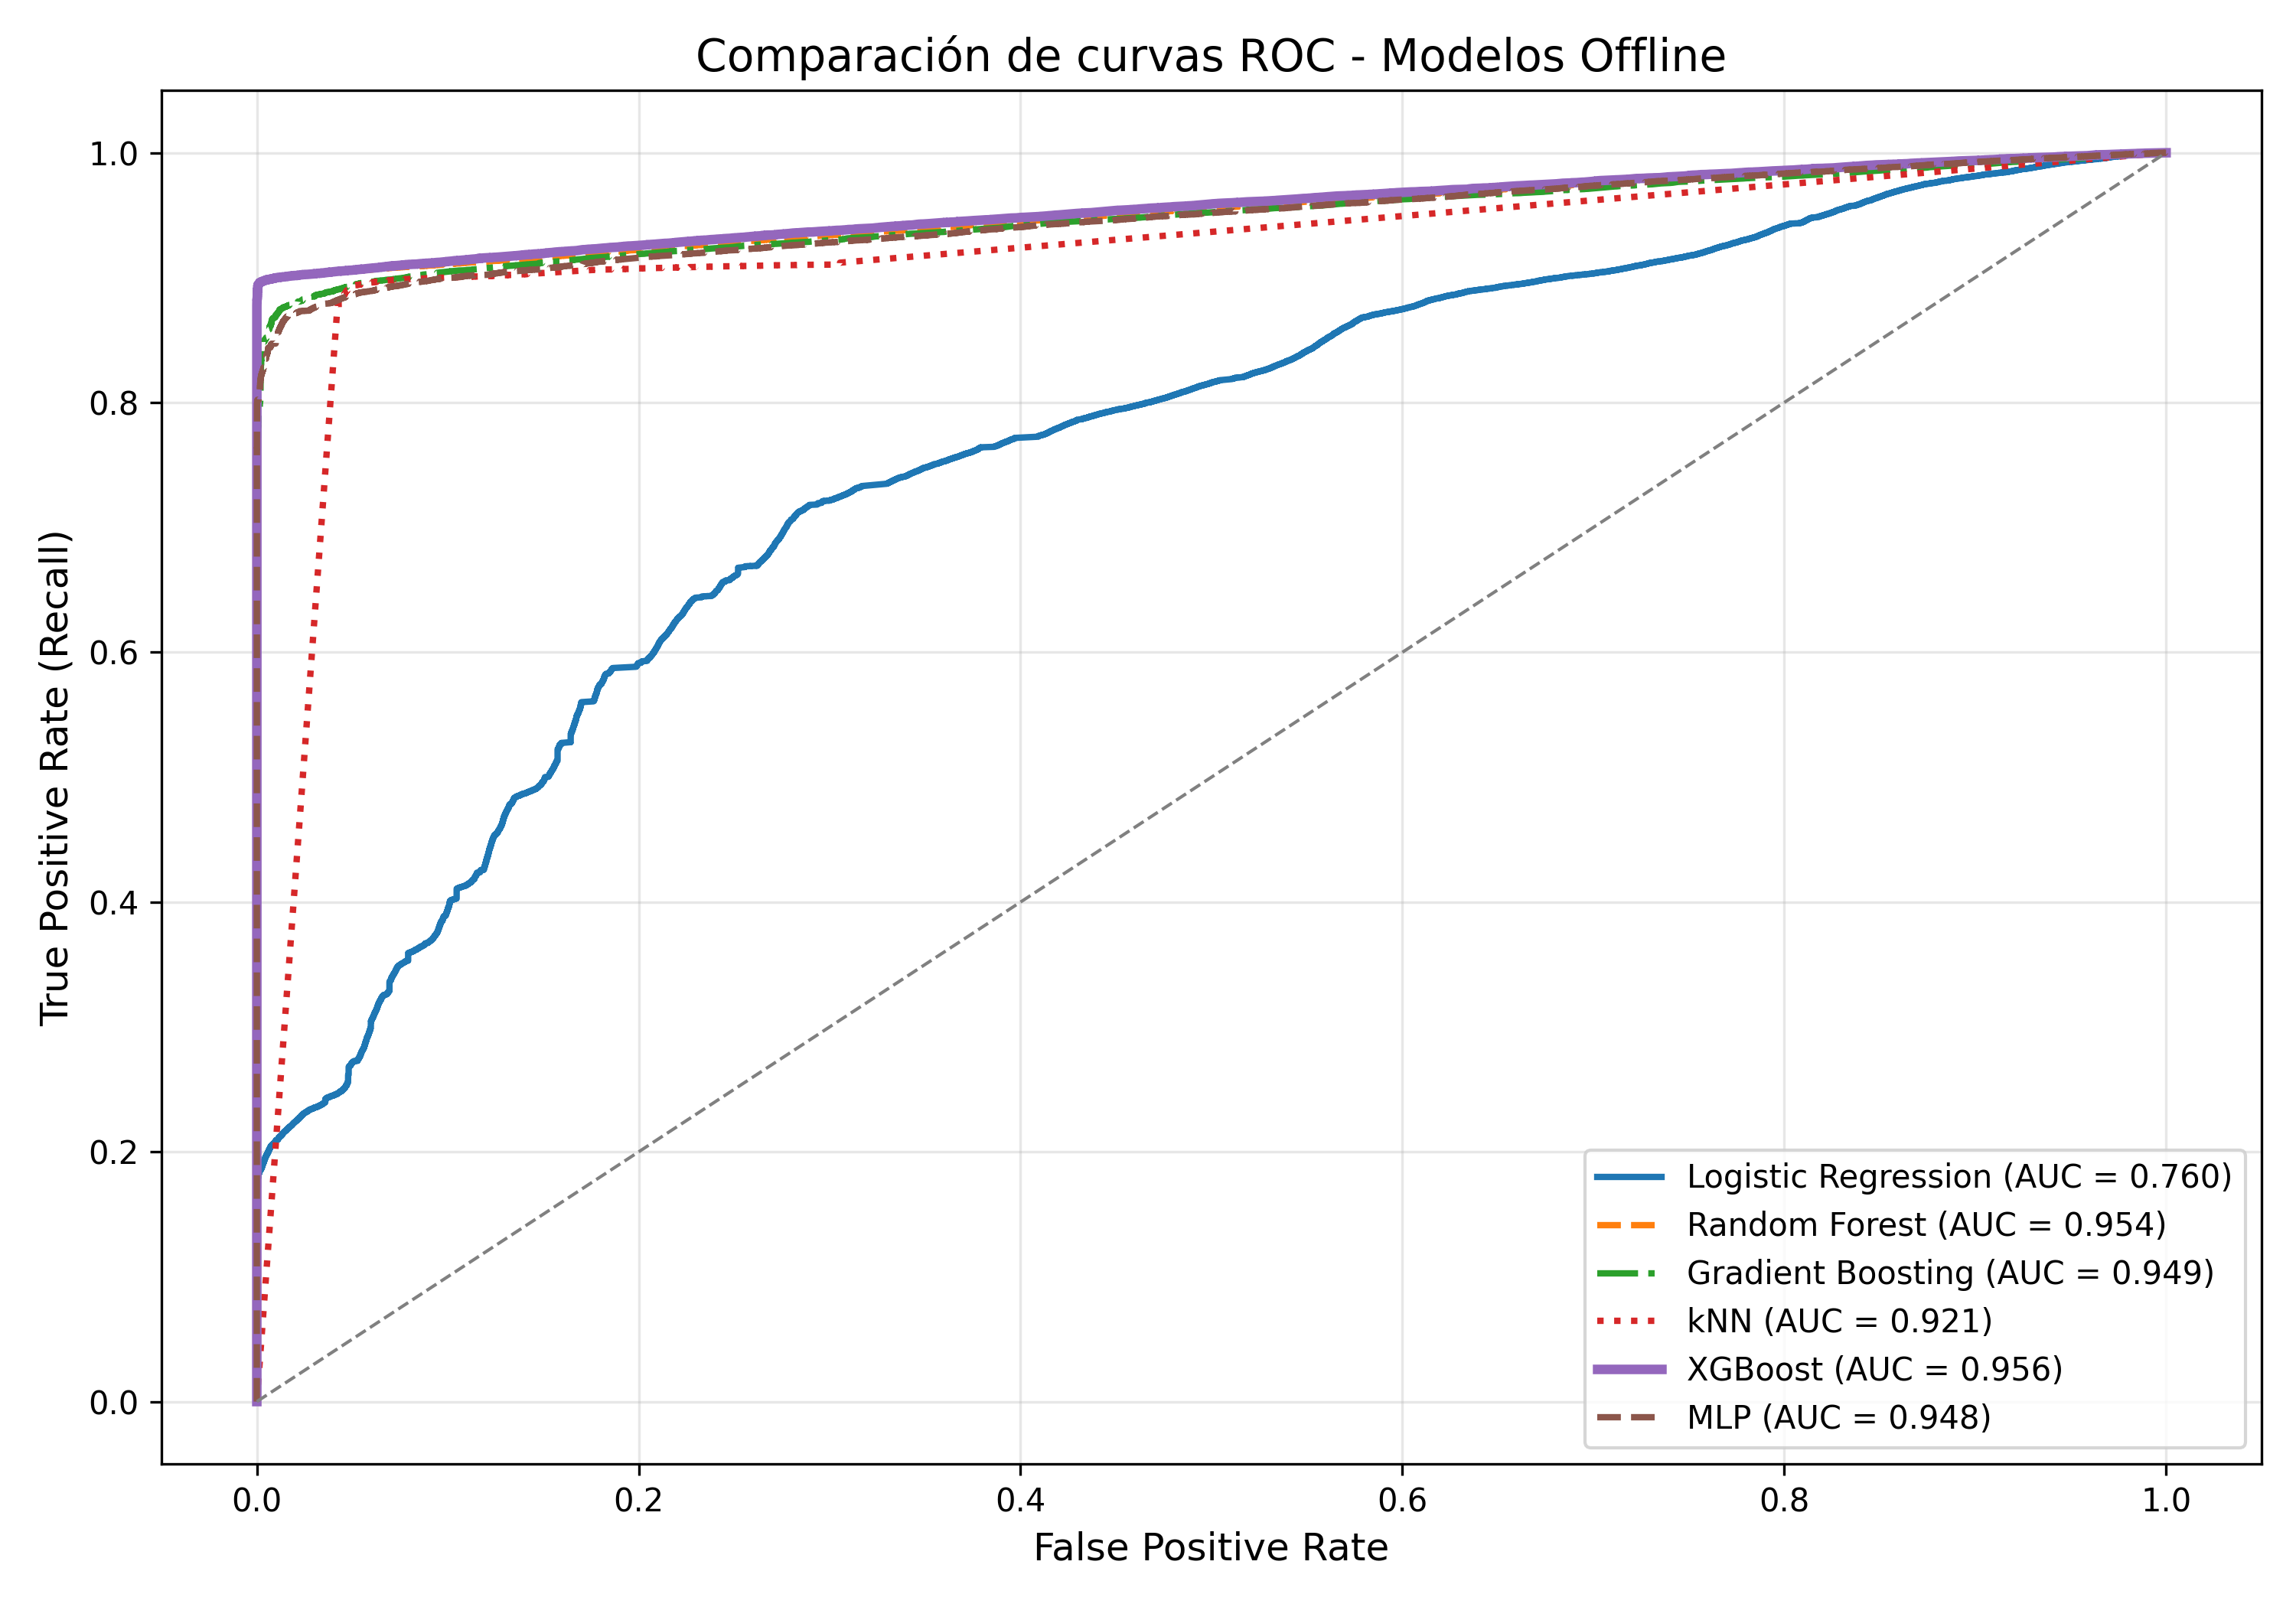
\includegraphics[width=0.95\textwidth]{imagenes/roc_comparison_offline.png}
    \caption{Curvas ROC Métodos \emph{Offline}.}
    \label{fig:roc_offline}
\end{figure}

\begin{figure}[H]
    \centering
    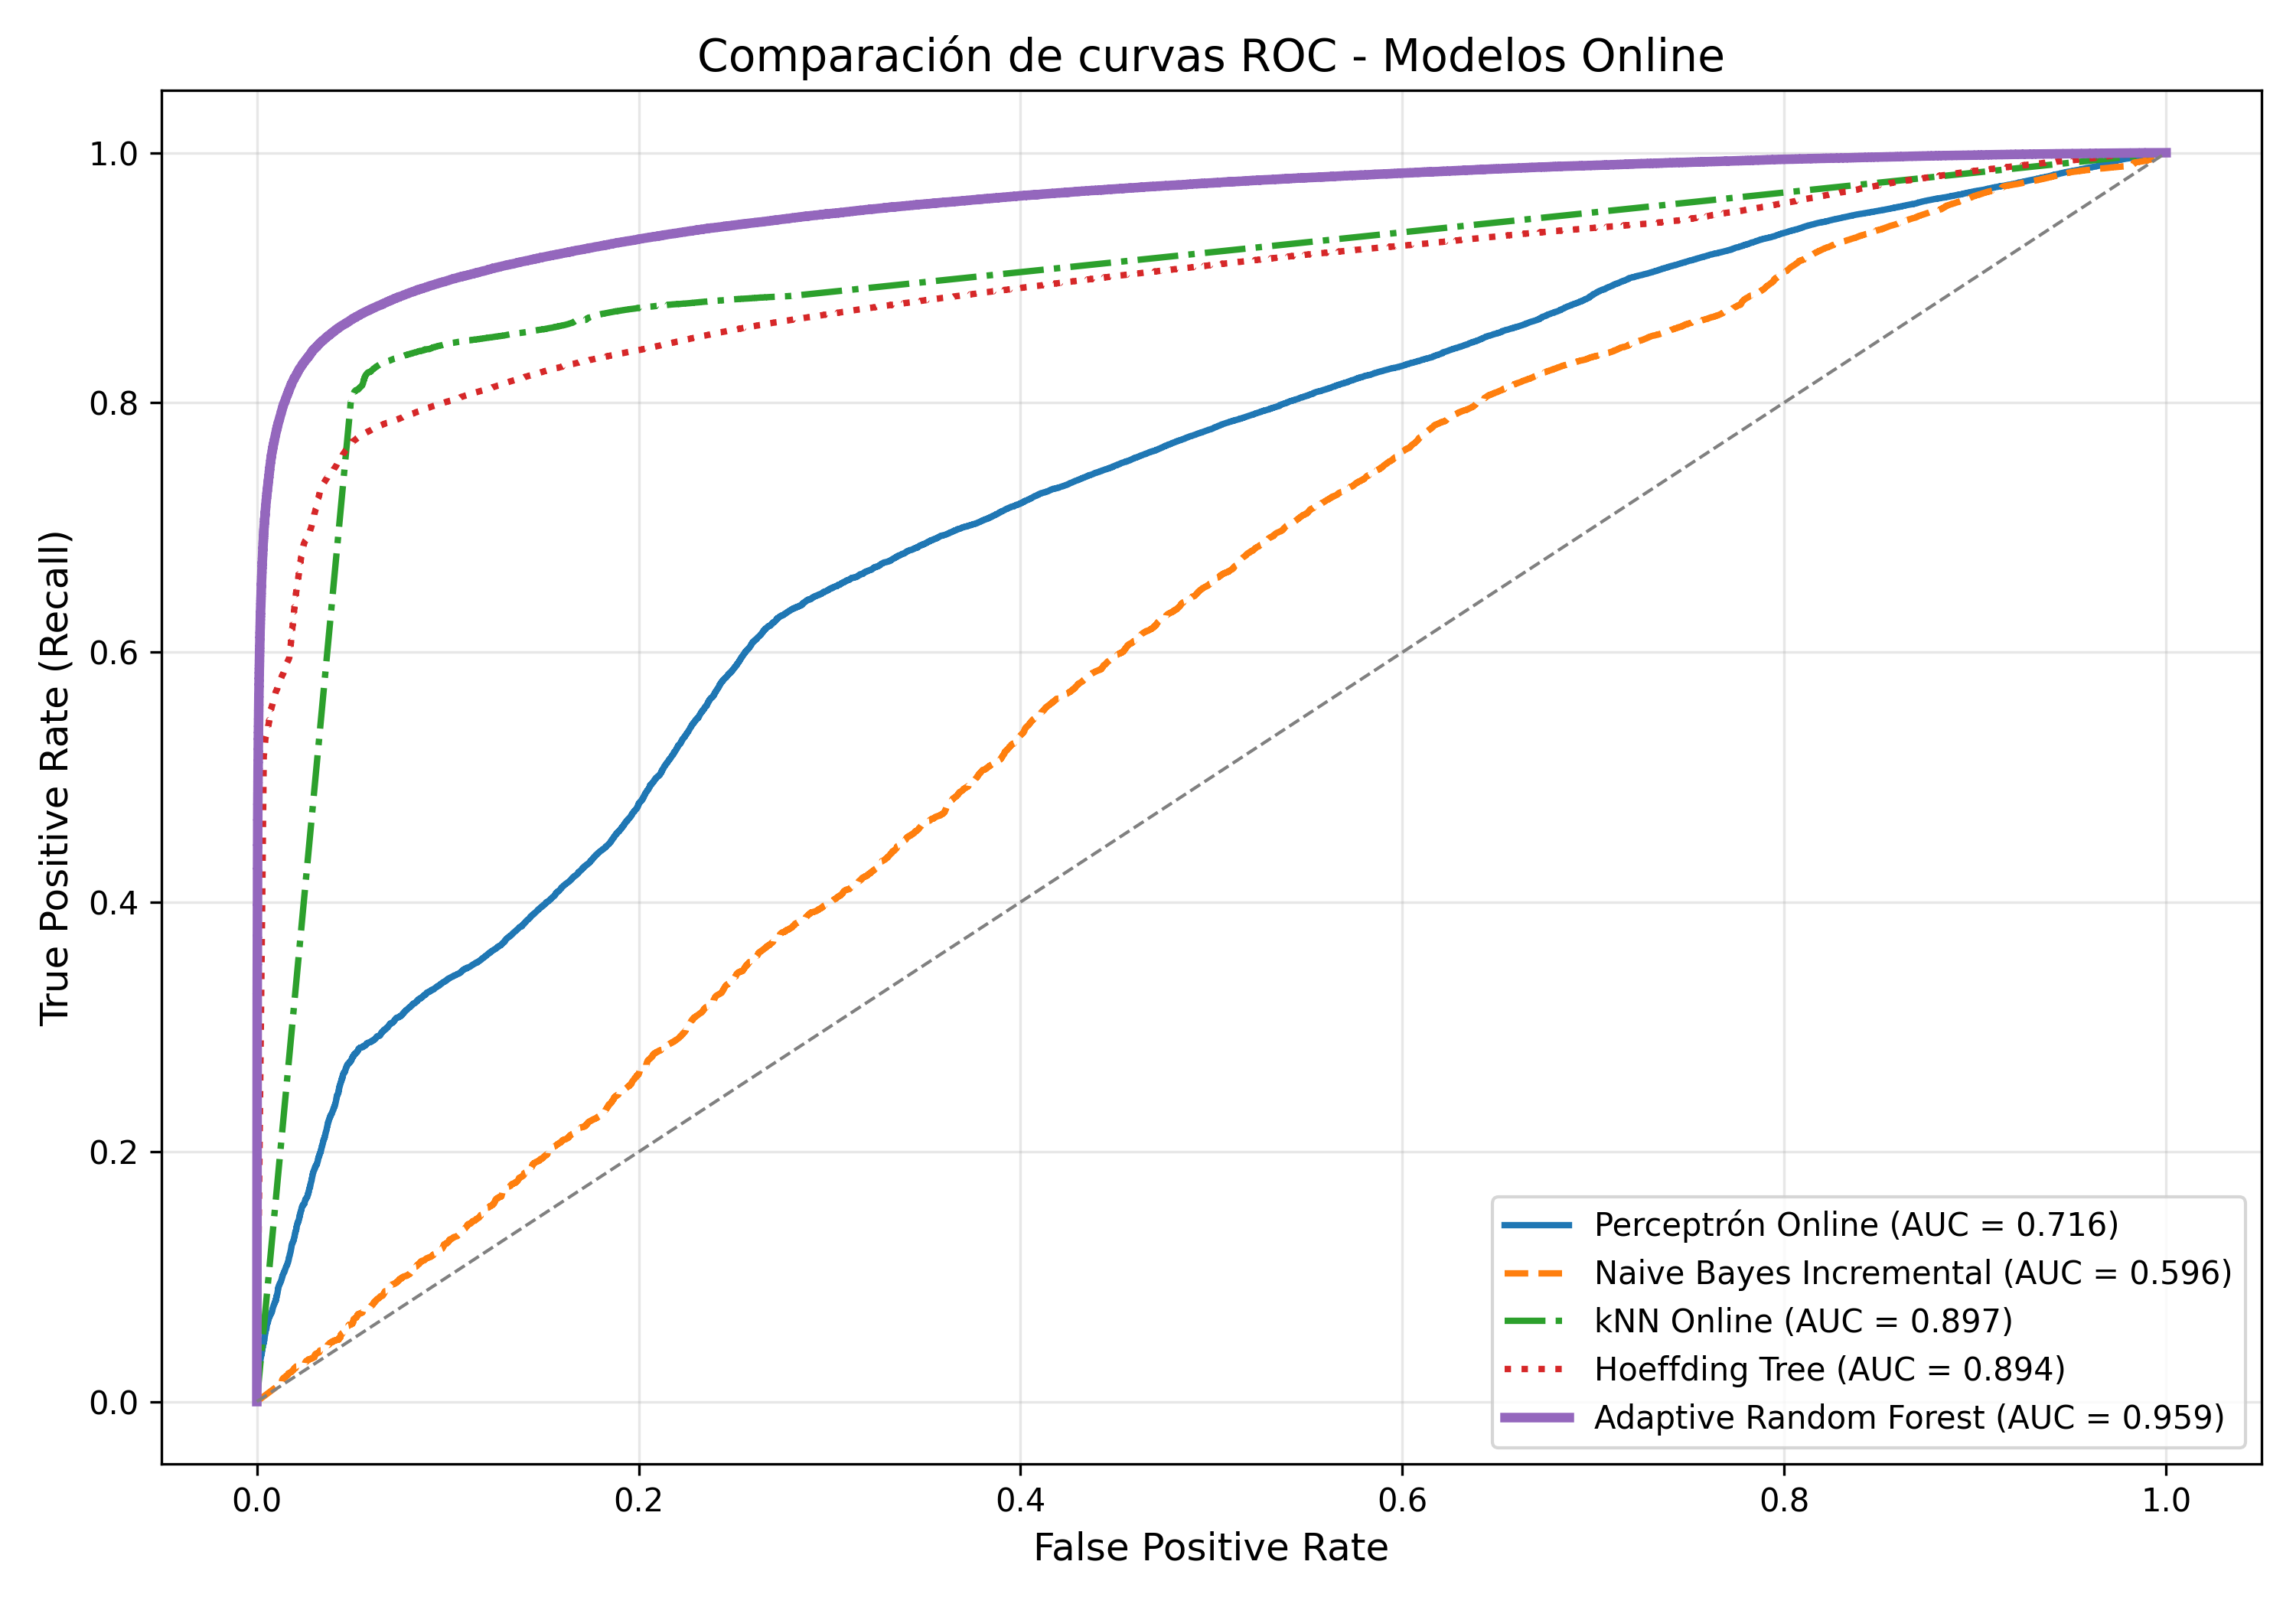
\includegraphics[width=0.95\textwidth]{imagenes/roc_comparison_online.png}
    \caption{Curvas ROC Métodos \emph{Online}.}
    \label{fig:roc_online}
\end{figure}

Para terminar de mostrar resultados, se añade la influencia de las variables en la detección de fraude eléctrico, con la que se estudia la importancia de características obtenida mediante los modelos \emph{Random Forest}, \emph{Gradient Boosting} y \emph{XGBoost}.

\begin{figure}[H]
\centering
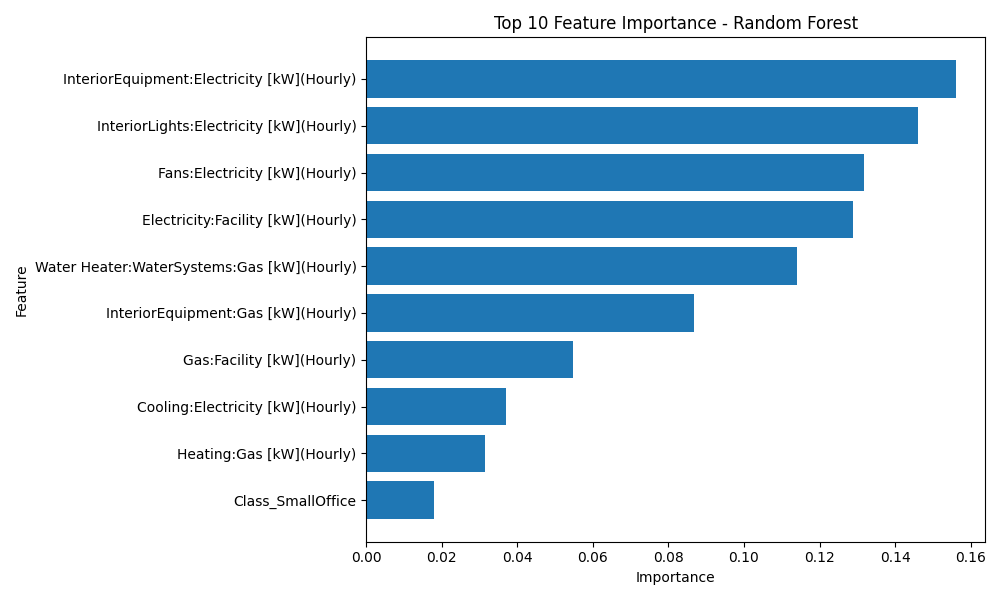
\includegraphics[width=0.95\textwidth]{imagenes/random_forest_feature_importance.png}
\caption{Importancia de variables obtenida con \emph{Random Forest}.}
\end{figure}

\begin{figure}[H]
\centering
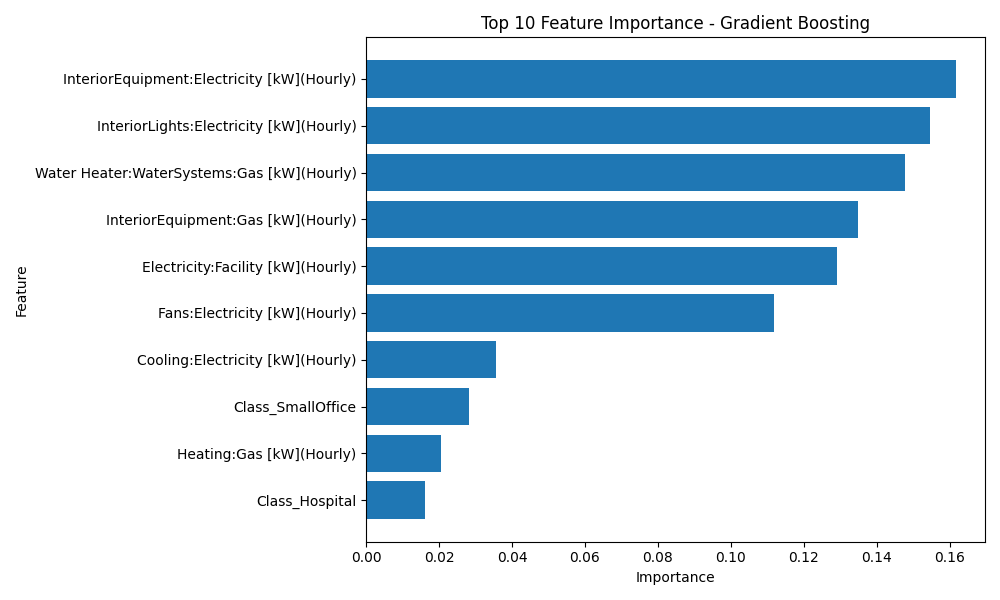
\includegraphics[width=0.95\textwidth]{imagenes/gradient_boosting_feature_importance.png}
\caption{Importancia de variables obtenida con \emph{Gradient Boosting}.}
\end{figure}

\begin{figure}[H]
\centering
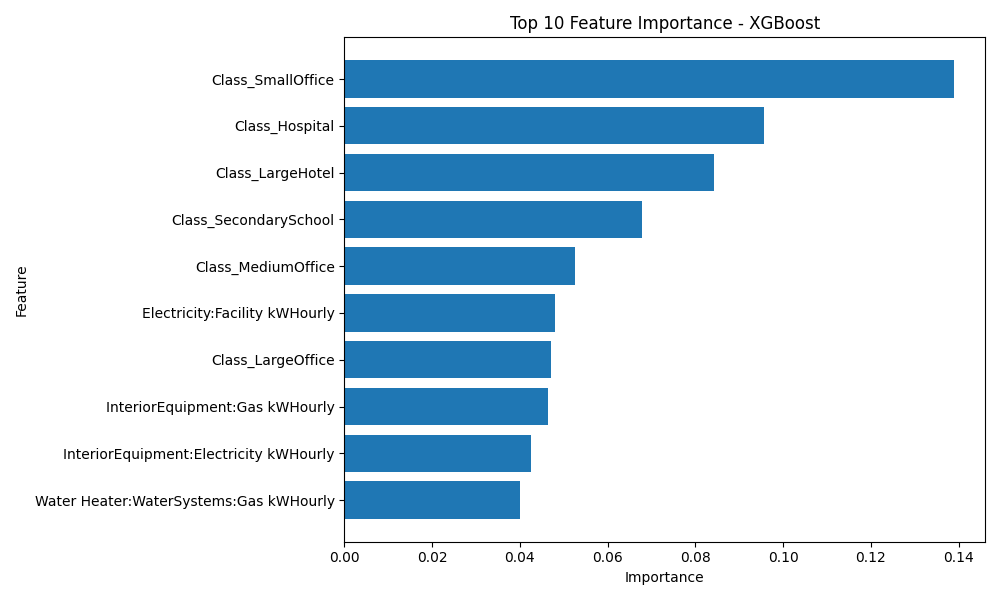
\includegraphics[width=0.95\textwidth]{imagenes/xgboost_feature_importance.png}
\caption{Importancia de variables obtenida con \emph{XGBoost}.}
\end{figure}


\section{Análisis y discusión de resultados}

En general, se observa un alto rendimiento en la mayoría de los modelos basados en técnicas de aprendizaje más avanzadas, mientras que los métodos más simples presentan un comportamiento claramente inferior. En primer lugar, la Regresión Logística muestra el peor rendimiento global, con una exactitud del 71.1\% y una puntuación F1 de 0.67. Aunque presenta un valor de \emph{recall} relativamente alto de 0.719, su baja precisión de 0.628 indica una mayor cantidad de falsos positivos. Esto se refleja también en una tasa de falsos positivos (FPR) bastante alta de 0.294 y un valor de ROC-AUC de 0.76, mostrando una capacidad limitada para distinguir entre las clases. Estos resultados indican que, si bien el modelo es capaz de detectar una parte considerable de los casos de fraude, lo hace a costa de generar un número elevado de clasificaciones erróneas.

Por otro lado, los modelos basados en técnicas de ensamble muestran un rendimiento notablemente superior. En el caso de \emph{Random Forest}, se obtiene una exactitud del 95.6\% y una puntuación F1 de 0.943, acompañado de una precisión prácticamente perfecta de 0.998. Este modelo presenta además una tasa de falsos positivos extremadamente baja de 0.001, lo que indica una gran capacidad para evitar clasificaciones incorrectas de la clase mayoritaria. Su valor ROC-AUC de 0.954 confirma su elevado poder discriminativo. De forma similar, el modelo \emph{Gradient Boosting} presenta un comportamiento muy competitivo, con una puntuación F1 de 0.924 y una ROC-AUC de 0.949. Aunque su precisión de 0.981 y su tasa de falsos positivos de 0.012 son ligeramente inferiores a las de \emph{Random Forest}, sigue mostrando un equilibrio adecuado entre precisión y capacidad de detección, reflejado en sus métricas globales.

El modelo kNN obtiene resultados algo inferiores en comparación con los métodos anteriores, con una puntuación F1 de 0.907 y una ROC-AUC de 0.921. Aunque mantiene un buen equilibrio entre precisión de 0.924 y \emph{recall} de 0.892, su tasa de falsos positivos de 0.051 es mayor, lo que indica una menor capacidad para discriminar correctamente en comparación con los modelos basados en árboles.

En cuanto al modelo \emph{XGBoost}, presenta el mejor rendimiento global entre todos los métodos evaluados. Destaca por obtener los valores más altos en prácticamente todas las métricas, incluyendo una exactitud del 95.7\%, una puntuación F1 de 0.944 y una ROC-AUC de 0.956. Además, combina una precisión casi perfecta de 0.999 con un elevado \emph{recall} de 0.895, manteniendo al mismo tiempo una tasa de falsos positivos mínima de 0.001. Estos resultados muestran una excelente capacidad para detectar casos de fraude minimizando los errores.

Finalmente, el Perceptrón Multicapa presenta un rendimiento competitivo, con una puntuación F1 de 0.918 y una ROC-AUC de 0.948. Aunque ligeramente inferior a los modelos de \emph{boosting}, muestra un comportamiento equilibrado entre precisión de 0.974 y \emph{recall} de 0.869, así como una baja tasa de falsos positivos de 0.016. Esto lo sitúa como una alternativa sólida dentro de los modelos evaluados. En conjunto, los resultados muestran una clara diferencia entre los modelos lineales y los modelos más complejos, siendo estos últimos los que alcanzan un mejor equilibrio entre las distintas métricas de evaluación.

Ahora se analiza más detalladamente las curvas ROC, en la Figura \ref{fig:roc_offline} se muestran las curvas ROC correspondientes a los modelos offline. Se observa que los modelos más avanzados, como XGBoost, Random Forest, Gradient Boosting y el Perceptrón Multicapa (MLP), presentan curvas muy próximas entre sí y cercanas al vértice superior izquierdo, lo que indica un rendimiento elevado y muy similar entre ellos. Esta superposición de curvas refleja que todos estos modelos poseen una alta capacidad de discriminación, alcanzando valores de ROC-AUC superiores a 0.94. En particular, XGBoost destaca ligeramente sobre el resto, obteniendo el mayor valor de AUC, lo que confirma su eficacia en la detección de fraude en este problema. Por otro lado, el modelo kNN presenta un rendimiento inferior, aunque sigue mostrando una capacidad discriminativa aceptable. Finalmente, la Regresión Logística presenta la curva más alejada del óptimo, lo que muestra un rendimiento bastante menor en comparación con los modelos más complejos.

En la Figura \ref{fig:roc_online}  se presentan las curvas ROC de los modelos online. A diferencia del caso \emph{offline}, en este escenario se observa una mayor separación entre las curvas, lo que permite distinguir con mayor claridad el rendimiento de cada algoritmo. El modelo \emph{Adaptive Random Forest} destaca claramente como el mejor método online, alcanzando el mayor valor de ROC-AUC y mostrando una curva más cercana al comportamiento óptimo. Le siguen el kNN \emph{online} y el \emph{Hoeffding Tree}, que presentan un rendimiento competitivo y relativamente similar. En contraste, el Perceptrón \emph{online} y el Naive Bayes incremental muestran un comportamiento notablemente inferior, especialmente este último, cuya curva se aproxima en mayor medida a la línea base, indicando una menor capacidad de discriminación.

Para terminar el estudio de los resultados, es el turno ahora de la importancia de las variables. Para ello se mostraron las gráficas de tres modelos en particular. En primer lugar, el modelo \emph{Random Forest} identifica como variables más relevantes aquellas relacionadas con el consumo eléctrico en distintos componentes del sistema. En particular, destacan  \emph{InteriorEquipment:Electricity},  \emph{InteriorLights:Electricity} y  \emph{Fans:Electricity}, lo que indica que el consumo energético interno del edificio es un factor clave en la detección de comportamientos anómalos. Además, variables relacionadas con el consumo de gas y agua, como  \emph{Water Heater:WaterSystems:Gas} e  \emph{InteriorEquipment:Gas}, también presentan una contribución significativa. Esto sugiere que el fraude no solo se manifiesta en el consumo eléctrico directo, sino también en patrones de consumo energético global.

En el caso de  \emph{Gradient Boosting}, se observa una distribución más concentrada en variables energéticas específicas. Las variables más influyentes corresponden principalmente al consumo eléctrico interno, destacando  \emph{InteriorEquipment:Electricity} e  \emph{InteriorLights:Electricity} como las más relevantes. A diferencia del modelo anterior, este modelo otorga menor importancia a variables categóricas como el tipo de edificio, lo que indica que el modelo prioriza patrones de consumo sobre características del usuario.

Finalmente, el modelo  \emph{XGBoost} presenta un comportamiento diferenciado respecto a los anteriores. En este caso, las variables más importantes están relacionadas con la tipología del edificio, como  \emph{Class\_SmallOffice},  \emph{Class\_Hospital} y  \emph{Class\_LargeHotel}. Esto indica que este modelo es capaz de capturar relaciones más complejas entre el tipo de instalación y la probabilidad de fraude, incorporando información estructural que otros modelos consideran menos relevante.

En conjunto, los resultados muestran que  \emph{Random Forest} y  \emph{Gradient Boosting} coinciden en otorgar mayor relevancia a variables relacionadas con el consumo energético. Mientras que  \emph{XGBoost}, incorpora con mayor peso variables categóricas relacionadas con el tipo de edificio. Sin embargo, es importante destacar que las medidas de importancia de variables pueden presentar sesgos, especialmente hacia variables con mayor variabilidad o número de categorías, por lo que estos resultados deben interpretarse con cautela.


\section{Conclusiones}

En este trabajo se realiza un estudio comparativo entre distintos modelos de aprendizaje automático, tanto en entornos \emph{offline} como \emph{online}, para detectar fraude en el consumo eléctrico. Con los resultados obtenidos se pueden extraer diversas conclusiones importantes sobre el rendimiento, la capacidad de generalización y la aplicabilidad de los modelos.

Los modelos \emph{offline} muestran un rendimiento superior al de los modelos \emph{online}. Esto se debe a que estos algoritmos disponen del conjunto completo de datos durante el entrenamiento, lo que les permite ajustar sus parámetros de forma más precisa y capturar relaciones complejas entre las variables. Destacan los modelos basados en técnicas de ensamble, como \emph{Random Forest}, \emph{Gradient Boosting}, \emph{XGBoost} y MLP. \emph{XGBoost} es el algoritmo con mejor rendimiento global, ya que combina una precisión alta con una capacidad alta de detección de fraude, manteniendo al mismo tiempo una tasa de falsos positivos muy pequeña. Esto puede explicarse por que está basado en \emph{boosting}, donde cada nuevo modelo corrige los errores de los anteriores, así como por la incorporación de mecanismos de regularización que evitan el sobreajuste. Los modelos más simples, como la Regresión Logística, presentan un rendimiento bastante inferior. Esto se debe a su capacidad limitada para modelar relaciones no lineales en los datos. Aunque este modelo se usa como una base simple para comparar el resto de modelos más avanzados, no resulta útil para la detección de fraude eléctrico.

En los modelos \emph{online} se observan comportamientos más variados. El modelo Adaptive Random Forest destaca por encima del resto. Este resultado demuestra que es posible obtener un rendimiento competitivo en escenarios de flujo de datos mediante el uso de técnicas de ensamble adaptativas. Los modelos como kNN \emph{online} y \emph{Hoeffding Tree} muestran un rendimiento aceptable, aunque inferior. Los modelos como Perceptrón online y el Naive Bayes incremental presentan limitaciones importantes, especialmente en la capacidad para distinguir entre comportamientos normales o fraudulentos. El bajo rendimiento de Naive Bayes se explica por la fuerte independencia entre variables, que no se cumple en el conjunto de datos utilizado.

Los resultados muestran que existe una relación entre rendimiento y capacidad de adaptación al flujo de datos. Mientras que los modelos \emph{offline} ofrecen mejores resultados en términos de precisión y capacidad para separar entre comportamientos normales o fraudes, los modelos \emph{online} permiten trabajar en entornos dinámicos donde los datos llegan de forma continua, lo que resulta muy importante en aplicaciones en tiempo real. Este estudio destaca la importancia de seleccionar el modelo adecuado en función del contexto del problema. En escenarios donde se dispone de todos los datos y se busca maximizar el rendimiento, modelos como \emph{XGBoost} resultan la mejor opción. Sin embargo, en entornos donde los datos se generan de forma continua, algoritmos como \emph{Adaptive Random Forest} ofrecen una alternativa eficaz, combinando adaptabilidad y un rendimiento competitivo.



% =========================
% CAPÍTULO 7
% =========================
\chapter{Requisitos del Sistema}

Para definir los requisitos del sistema del proyecto, se ha realizado un análisis del problema de detección de fraude en el consumo eléctrico y de las necesidades que tendría una empresa energética o analista encargado de supervisar los datos de consumo. El objetivo del sistema es proporcionar una herramienta que permita analizar datos de consumo energético y aplicar modelos de aprendizaje automático para detectar posibles casos de fraude. Además, se ofrece un entorno web que facilite la visualización de los resultados y la comparación entre distintos modelos de clasificación, permitiendo interpretar de forma clara el rendimiento de cada uno de ellos.


\section{Situación actual}

El fraude del consumo eléctrico es un problema importante para las compañías energéticas, porque provoca pérdidas económicas y puede afectar a la estabilidad de la red eléctrica. Gracias a los sistemas de medición inteligentes, existen cantidades grandes de datos del consumo energético de los usuarios. Sin embargo, analizar manualmente estos datos para identificar comportamientos que no son normales resulta una tarea difícil. El uso de técnicas de aprendizaje automático son una alternativa eficaz para detectar patrones de comportamiento que puedan indicar fraude.


\section{Entorno Tecnológico}

El sistema se basa en un entorno web implementado en Python, que permite ejecutar modelos de aprendizaje automático y ver los resultados obtenidos de forma clara. El entorno tecnológico necesario para el uso del sistema incluye un ordenador con acceso a Internet, un navegador web moderno y, un servidor donde se ejecute el entorno web y los modelos de aprendizaje automático. Para que el sistema funcione no se necesita un \emph{hardware} específico por parte del usuario, ya que los modelos de aprendizaje automático se ejecutan en el servidor y los usuarios interactúan con el sistema a través de la interfaz web.

Las tecnologías utilizadas en el desarrollo del sistema incluyen: Python como lenguaje principal de programación, Scikit-learn para la implementación de los modelos de aprendizaje automático, Pandas y NumPy para el procesamiento y análisis de los datos y FastApi como framework web en Python utilizado para la creación del entorno web. Este conjunto de tecnologías permite desarrollar una solución flexible y fácilmente extensible, facilitando la experimentación con distintos modelos de detección de fraude en el consumo eléctrico.


\section{Fortalezas y Debilidades}

La habilidad para examinar grandes volúmenes de datos sobre el consumo eléctrico y descubrir posibles patrones de fraude, empleando métodos de aprendizaje automático, es el principal punto fuerte del sistema. El sistema posibilita, además, el análisis comparativo de varios modelos de clasificación y la visualización de sus métricas de rendimiento, lo que simplifica la evaluación sobre cuáles algoritmos son más efectivos para resolver el problema. La presencia de un entorno en la web que centraliza la implementación de los modelos y la visualización de resultados, lo que posibilita a los usuarios llevar a cabo un análisis intuitivo de la información, es otra ventaja relevante.

No obstante, el sistema también tiene ciertas limitaciones. La calidad y la representatividad de los datos empleados para entrenar los modelos son el primer elemento que define lo buenos que serán los resultados. Asimismo, los modelos de aprendizaje automático tienen la capacidad de producir falsos negativos o falsos positivos. Esto significa que el sistema debe ser utilizado como una herramienta adicional al análisis y no como un mecanismo de decisión totalmente determinante. Por último, el primer despliegue del sistema incorpora una cantidad restringida de modelos. Por lo tanto, será imprescindible continuar con la investigación y la prueba de procedimientos innovadores para aumentar su exactitud.


\section{Necesidades de Negocio}

El propósito fundamental del sistema es ofrecer un instrumento que facilite el análisis de datos sobre consumo de energía y la identificación automática de potenciales fraudes eléctricos. Para poder llevar a cabo inspecciones o investigaciones más exhaustivas, las compañías energéticas requieren detectar de manera rápida comportamientos anómalos en el consumo.


\subsection{Objetivos de Negocio}

El sistema creado tiene como objetivo simplificar el proceso de negocio a través del empleo de modelos de aprendizaje automático que posibiliten la categorización de los registros de consumo en normales o fraudulentos. El sistema también tiene que posibilitar la comparación del desempeño de diferentes modelos de clasificación y la visualización de los resultados logrados. Todo esto se verá reflejado en una interfaz web que haga más fácil ver los resultados y las métricas de evaluación. El sistema posibilita un análisis de los datos más eficaz que el de las técnicas tradicionales que solo se fundamentan en inspecciones manuales.


\subsection{Procesos de Negocio}

El sistema funciona en distintas fases. Primero, se carga el conjunto de datos que contiene información sobre el consumo eléctrico. En segundo lugar, el preprocesamiento de la información, que abarca la depuración de los registros, la conversión de variables categóricas y el acondicionamiento de los datos para su aplicación en modelos. Tercero: el entrenamiento de modelos de clasificación, que estudian los patrones en el consumo eléctrico y aprenden a diferenciar entre comportamientos fraudulentos y normales. Cuarto, la valoración de los modelos, empleando diferentes métricas como precisión, exactitud, Kappa de Cohen, matriz de confusión, F1-score y recall. Finalmente, la visualización de resultados en el ambiente web, donde los usuarios tienen la posibilidad de verificar las métricas del rendimiento y contrastar las diferentes categorías de los modelos. Además, se seleccionan los que ofrecen mejores resultados de cada categoría.


\section{Catálogo de Requisitos del Sistema}


\subsection{Requisitos funcionales}

Los requisitos funcionales describen las funcionalidades que el sistema debe proporcionar a los usuarios.

\begin{table}[H]
\centering
\begin{tabular}{|p{2cm}|p{5cm}|p{7cm}|}
\hline
\textbf{ID} & \textbf{Nombre} & \textbf{Descripción} \\ \hline

RF1 & Carga de datos de consumo eléctrico. & El sistema debe permitir cargar un conjunto de datos que contenga información sobre el consumo eléctrico de los usuarios. \\ \hline

RF2 & Preprocesamiento automático de datos. & El sistema debe realizar automáticamente el preprocesamiento de los datos, incluyendo limpieza de datos, transformación de variables categóricas y preparación del conjunto de datos para su uso en modelos de aprendizaje automático. \\ \hline

RF3 & Entrenamiento de modelos. & El sistema debe permitir entrenar distintos modelos de clasificación utilizando los datos disponibles para detectar posibles casos de fraude en el consumo eléctrico. \\ \hline

RF4 & Evaluación del rendimiento de los modelos. & El sistema debe calcular métricas de evaluación para los modelos entrenados, tales como accuracy, precision, recall, F1-score, matriz de confusión y Cohen’s Kappa. \\ \hline

RF5 & Validación cruzada de modelos. & El sistema debe permitir realizar validación cruzada para evaluar la estabilidad de los modelos entrenados. \\ \hline

RF6 & Visualización de resultados. & El sistema debe mostrar los resultados obtenidos por los modelos a través del entorno web, incluyendo métricas de rendimiento. \\ \hline

RF7 & Comparación entre modelos. & El sistema debe permitir comparar el rendimiento de diferentes modelos para identificar cuál ofrece mejores resultados en la detección de fraude. \\ \hline

RF8 & Consulta de resultados almacenados. & El sistema debe permitir consultar los resultados obtenidos en experimentos previos, almacenados en archivos o base de datos. \\ \hline

RF9 & Autenticación de usuarios. & El sistema debe permitir a los usuarios registrarse e iniciar sesión para acceder a las funcionalidades del entorno web. \\ \hline

\end{tabular}
\caption{Requisitos funcionales del sistema}
\end{table}


\subsection{Requisitos no funcionales}

Los requisitos no funcionales describen características del sistema relacionadas con rendimiento, usabilidad, seguridad o escalabilidad.

\begin{table}[H]
\centering
\begin{tabular}{|p{2cm}|p{5cm}|p{7cm}|}
\hline
\textbf{ID} & \textbf{Nombre} & \textbf{Descripción} \\ \hline

RNF1 & Rendimiento. & El sistema debe ser capaz de procesar grandes volúmenes de datos de consumo eléctrico en un tiempo razonable. \\ \hline

RNF2 & Escalabilidad. & La arquitectura del sistema debe permitir la incorporación de nuevos modelos de aprendizaje automático en el futuro sin necesidad de modificar significativamente el sistema existente. \\ \hline

RNF3 & Usabilidad. & La interfaz web debe ser sencilla e intuitiva, permitiendo a los usuarios consultar resultados y métricas sin necesidad de conocimientos avanzados de programación. \\ \hline

RNF4 & Accesibilidad. & El sistema debe ser accesible a través de navegadores web estándar sin necesidad de instalar software adicional. \\ \hline

RNF5 & Mantenibilidad. & El código del sistema debe estar organizado y documentado para facilitar futuras modificaciones o mejoras. \\ \hline

RNF6 & Fiabilidad. & El sistema debe proporcionar resultados consistentes cuando se ejecutan los mismos modelos con los mismos datos. \\ \hline

\end{tabular}
\caption{Requisitos no funcionales del sistema}
\end{table}


\subsection{Requisitos de información}

Los requisitos de información describen los tipos de datos que el sistema debe gestionar para su correcto funcionamiento.

\begin{table}[H]
\centering
\begin{tabular}{|p{2cm}|p{5cm}|p{7cm}|}
\hline
\textbf{ID} & \textbf{Nombre} & \textbf{Descripción} \\ \hline

RI1 & Datos de consumo energético. & El sistema debe gestionar datos relacionados con el consumo eléctrico utilizados para el entrenamiento y evaluación de los modelos. \\ \hline

RI2 & Etiquetas de clasificación. & El sistema debe manejar una variable objetivo que indique si un registro corresponde a consumo normal o a un posible caso de fraude eléctrico, permitiendo entrenar modelos de clasificación. \\ \hline

RI3 & Resultados de los modelos. & El sistema debe almacenar los resultados obtenidos tras el entrenamiento de los modelos, incluyendo métricas de evaluación como accuracy, precision, recall, F1-score, matriz de confusión y Cohen's Kappa. \\ \hline

RI4 & Datos de experimentación. & El sistema debe registrar los resultados de los diferentes experimentos realizados con los modelos, permitiendo comparar el rendimiento de distintos algoritmos. \\ \hline

RI5 & Datos de usuarios del sistema. & El sistema debe almacenar información básica de los usuarios registrados que acceden al entorno web, con el objetivo de gestionar el acceso al sistema. \\ \hline

RI6 & Protección de datos. & Los datos de los usuarios del sistema se almacenarán de forma segura, aplicando técnicas de cifrado para las contraseñas y limitando su uso únicamente a la gestión de autenticación y acceso al sistema. No se utilizarán estos datos para otros fines ni se compartirán con terceros. \\ \hline

\end{tabular}
\caption{Requisitos de información del sistema}
\end{table}



% =========================
% CAPÍTULO 8
% =========================
\chapter{Análisis del Sistema}


\section{Objetivo del prototipo software}

Se propone el diseño de un prototipo de software que haga posible utilizar los resultados obtenidos en un ambiente funcional, tras llevar a cabo la etapa experimental, donde se ponen en práctica y analizan diversos modelos de aprendizaje automático para identificar el fraude eléctrico. El propósito fundamental del prototipo es ayudar a un operador de una compañía eléctrica a importar las curvas de consumo y clasificar automáticamente cada registro como posible fraude o consumo normal; para ello, se emplean los modelos que ya fueron entrenados y que han demostrado un mejor desempeño en la comparación experimental. El prototipo, además de su función principal, ofrece la posibilidad de comparar ambas categorías de manera objetiva y ver recursos gráficos como las curvas ROC o el valor que tienen las variables en la predicción. 

El sistema emplea modelos que ya fueron entrenados y guardados, en lugar de reentrenarlos en tiempo real. Esta decisión posibilita disminuir el costo computacional, mejorar la velocidad de respuesta del prototipo y distinguir con claridad entre la fase experimental y la fase operativa. Por lo tanto, los modelos se entrenan y evalúan antes a través de scripts experimentales, mientras que la aplicación se enfoca en consultar resultados y crear predicciones basadas en datos nuevos importados.

\section{Modelo conceptual del sistema}

El modelo conceptual del sistema se desarrolla considerando las etapas operativa y experimental del prototipo. La entidad \emph{ModeloPredictivo} es un reflejo de los modelos que han sido entrenados y analizados, los cuales se dividen en modelos \emph{online} y \emph{offline} a través de la entidad \emph{CategoriaModelo}. Cada modelo cuenta con un resultado de evaluación vinculado, curvas ROC y detalles acerca de la relevancia de las variables en los casos en que el algoritmo lo permite. En cambio, la entidad \emph{ArchivoConsumo} contiene el archivo CSV que el operador ha importado, que consta de una o varias \emph{CurvaConsumo}. Cada curva puede ser analizada por uno de los modelos entrenados, creando una entidad llamada \emph{Predicción}, que guarda la fecha en la que se realiza la clasificación. Además, hay que destacar la clase Usuario que es el operador que realiza una predicción importando archivos de consumo.

\begin{figure}[H]
\centering
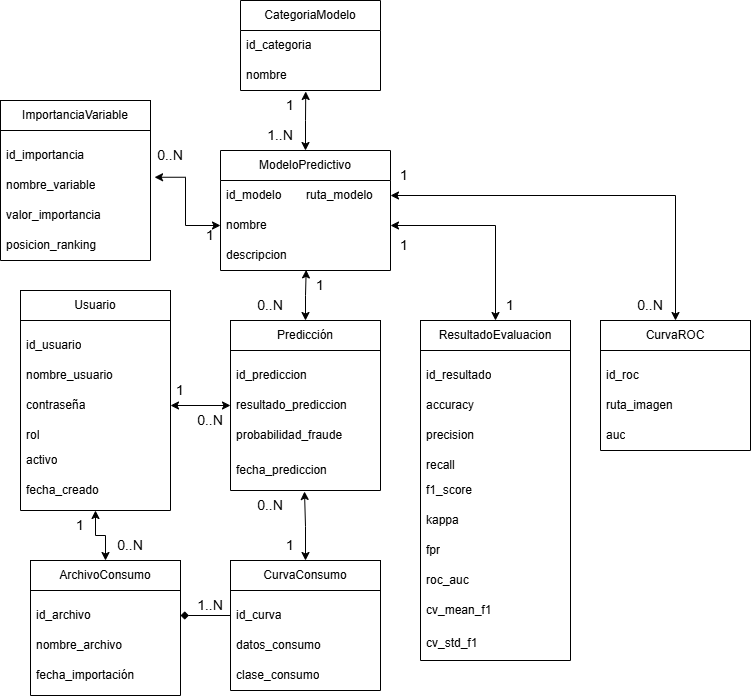
\includegraphics[width=0.95\textwidth]{imagenes/mcd_TFG.png}
\caption{Modelo Conceptual de Datos del sistema.}
\end{figure}


\section{Actores del sistema}

Los dos actores son el administrador del sistema y el operador de la compañía eléctrica. El primero representa al usuario funcional de la aplicación y el segundo se ocupa de las tareas técnicas requeridas para su implementación y mantenimiento.

El actor principal del sistema es el operador de la compañía eléctrica. Es el usuario que tiene la responsabilidad de manejar la aplicación con el fin de importar curvas de consumo eléctrico y conseguir una predicción para cada una, señalando si el uso está dentro de lo habitual o si podría haber un caso potencial de fraude. Su interacción con el sistema se enfoca en la fase operativa, o sea, en implementar los modelos escogidos a datos de consumo recientes. Entre sus principales responsabilidades están: llevar a cabo la clasificación de las curvas de consumo de un archivo importado, señalando si cada una es normal o indica posible fraude, así como la probabilidad vinculada a la predicción; revisar información adicional sobre los modelos que se emplean, como métricas de evaluación o curvas ROC, consultar el último resultado de predicción e iniciar sesión en el sistema.

El administrador del sistema es el actor encargado de gestionar los aspectos técnicos del prototipo. Su tarea principal es asegurar que el sistema esté listo para hacer predicciones con los modelos previamente entrenados, así como también que esté disponible y bien configurado. Dentro del marco de este proyecto, el administrador es el mismo que el creador del sistema; sin embargo, se distingue del operador debido a la clase de tareas que lleva a cabo. Entre las tareas fundamentales que realiza, están la gestión de los usuarios del sistema y la administración de los modelos entrenados y los resultados obtenidos durante las pruebas.


\section{Casos de Uso}

En esta sección se definen los principales casos de uso del sistema a partir de los actores anteriores. 

\begin{figure}[H]
\centering
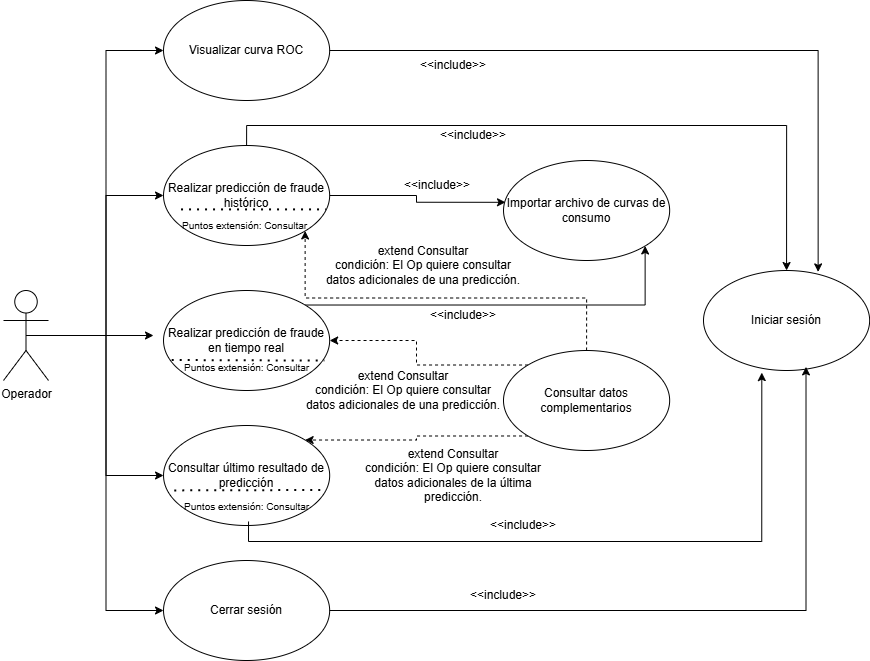
\includegraphics[width=0.95\textwidth]{imagenes/cuOp.png}
\caption{Diagrama de Casos de Uso del Operador del sistema.}
\end{figure}

\medskip

\begin{figure}[H]
\centering
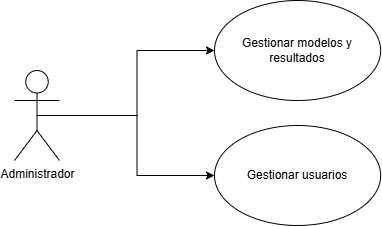
\includegraphics[width=0.75\textwidth]{imagenes/cuAd.png}
\caption{Diagrama de Casos de Uso del Administrador del sistema.}
\end{figure}

El diagrama muestra que el operador tiene que iniciar sesión para entrar al sistema. Su función principal es la elaboración de una predicción de fraude, lo que conlleva importar un archivo CSV que contenga curvas de consumo de electricidad. Este tiene dos opciones dependiendo si quiere una predicción histórica de los datos o en tiempo real para ir actualizando datos. Después de hacer la predicción, el operador tiene la posibilidad de revisar el resultado más reciente que se obtuvo y, si lo desea, entrar a datos adicionales que faciliten comprender la decisión del modelo, como métricas, curvas ROC o relevancia de variables.

Para el administrador, se han identificado dos principales casos de uso que tienen como objetivo la conservación del sistema. El primero implica la administración de modelos y resultados, lo que posibilita añadir nuevos modelos entrenados, actualizar los existentes o cambiar los archivos de resultados experimentales, métricas y recursos gráficos relacionados. El segundo caso de uso tiene que ver con la administración de usuarios, a través de la cual el administrador tiene la capacidad de crear, modificar o borrar usuarios y manejar sus permisos para acceder. Estos casos de uso, que son tareas de mantenimiento y configuración esenciales para asegurar un funcionamiento adecuado, no se incluyen en el flujo principal del sistema.


\subsection{Descripción de escenarios del operador}

A continuación, se desarrolla la descripción de los escenarios de casos de uso del operador. Para todos los casos de uso asociados al operador se considera como precondición que el usuario ha iniciado sesión correctamente en el sistema. Por tanto, el caso de uso \emph{Iniciar sesión} no se repite en la descripción de cada escenario, aunque se entiende como requisito previo para acceder a las funcionalidades del sistema.

\subsubsection{Realizar predicción de fraude histórica}

\noindent Primer Caso de Uso: Realizar predicción de fraude histórica.

\begin{itemize}[leftmargin=1.5cm]
    \item Escenario principal (éxito): Realizar predicción de fraude histórica.
    \item Escenario alternativo (error): Error en la introducción de los parámetros de la predicción.
    \item Escenario alternativo (error): El modelo entrenado necesario para realizar la predicción no está disponible.
    \item Escenario alternativo (error): Error durante el preprocesamiento de los datos.
    \item Escenario alternativo (excepción): El operador cancela la predicción.
\end{itemize}

\medskip

\noindent Escenario principal (éxito): Realizar predicción de fraude histórica.

\begin{enumerate}[leftmargin=1.5cm]
    \item El operador selecciona la opción realizar predicción de fraude histórica.
    \item El operador elige los parámetros que tendrán la predicción. Estos son el límite de registros y el límite de predicciones individuales mostradas en la respuesta.
    \item Se incluye el caso de uso \emph{Importar archivo de curvas de consumo}.
    \item Opcionalmente, se extiende el caso de uso \emph{Consultar datos complementarios}.
    \item El operador confirma la predicción de fraude del archivo importado.
    \item El sistema comprueba que los parámetros de la predicción son valores correctos.
    \item El sistema carga los modelos entrenados seleccionados para realizar la predicción.
    \item El sistema aplica el preprocesamiento necesario a las curvas de consumo importadas.
    \item El sistema realiza la predicción sobre las curvas de consumo. En este caso del modelo \emph{offline}, la predicción se realiza sobre el conjunto completo de datos.
    \item El sistema muestra por pantalla el resultado de cada curva, indicando si corresponde a consumo normal o posible fraude.
    \item El sistema muestra la probabilidad asociada a la predicción de fraude cuando esté disponible.
\end{enumerate}
\medskip

\noindent Extensiones:

6a. Error en la introducción de los parámetros de la predicción.
\begin{enumerate}[leftmargin=1.5cm]
    \item El sistema detecta que existe un error en algún parámetro de la predicción que el operador introdujo.
    \item El sistema muestra un mensaje de error indicando el error de ese parámetro en cuestión y no se realiza la predicción.
\end{enumerate}

\medskip

7a. Modelo entrenado no disponible.
\begin{enumerate}[leftmargin=1.5cm]
    \item El sistema detecta que el modelo \emph{offline} no existe o no está disponible en la ruta configurada.
    \item El sistema muestra un mensaje de error indicando que no es posible realizar la predicción y no se realiza la predicción.
\end{enumerate}

\medskip

8a. Error durante el preprocesamiento de los datos.
\begin{enumerate}[leftmargin=1.5cm]
    \item El sistema detecta que faltan columnas necesarias o que existen valores no válidos.
    \item El sistema muestra un mensaje de error indicando que los datos importados no son compatibles con el modelo y no se realiza la predicción.
\end{enumerate}

\medskip

1a-4a. Cancelar realizar predicción de fraude histórica.
\begin{enumerate}[leftmargin=1.5cm]
    \item El operador selecciona cancelar la predicción antes de confirmar.
    \item El sistema cancela la predicción.
\end{enumerate}

\medskip

\subsubsection{Realizar predicción de fraude en tiempo real}

\noindent Segundo Caso de Uso: Realizar predicción de fraude en tiempo real.

\begin{itemize}[leftmargin=1.5cm]
    \item Escenario principal (éxito): Realizar predicción de fraude en tiempo real.
    \item Escenario alternativo (error): Error en la introducción de los parámetros de la predicción.
    \item Escenario alternativo (error): El modelo entrenado necesario para realizar la predicción no está disponible.
    \item Escenario alternativo (error): Error durante el preprocesamiento de los datos.
    \item Escenario alternativo (error): El flujo online no puede simularse correctamente.
    \item Escenario alternativo (excepción): El operador cancela la predicción.
\end{itemize}

\medskip

\noindent Escenario principal (éxito): Realizar predicción de fraude en tiempo real.

\begin{enumerate}[leftmargin=1.5cm]
    \item El operador selecciona la opción realizar predicción de fraude en tiempo real.
    \item El operador elige los parámetros que tendrán la predicción. Estos son los intervalos de segundo, el límite de registros y el límite de predicciones individuales mostradas en la respuesta.
    \item Se incluye el caso de uso \emph{Importar archivo de curvas de consumo}.
    \item Opcionalmente, se extiende el caso de uso \emph{Consultar datos complementarios}.
    \item El operador confirma la predicción de fraude del archivo importado.
    \item El sistema comprueba que los parámetros de la predicción son valores correctos.
    \item El sistema carga los modelos entrenados seleccionados para realizar la predicción.
    \item El sistema aplica el preprocesamiento necesario a las curvas de consumo importadas.
    \item El sistema realiza la predicción sobre las curvas de consumo. En este caso del modelo \emph{online}, las curvas se procesan de forma secuencial simulando un flujo de datos.
    \item El sistema muestra por pantalla el resultado de cada curva, indicando si corresponde a consumo normal o posible fraude.
    \item El sistema muestra la probabilidad asociada a la predicción de fraude cuando esté disponible.
\end{enumerate}
\medskip

\noindent Extensiones:

6a. Error en la introducción de los parámetros de la predicción.
\begin{enumerate}[leftmargin=1.5cm]
    \item El sistema detecta que existe un error en algún parámetro de la predicción que el operador introdujo.
    \item El sistema muestra un mensaje de error indicando el error de ese parámetro en cuestión y no se realiza la predicción.
\end{enumerate}

\medskip

7a. Modelo entrenado no disponible.
\begin{enumerate}[leftmargin=1.5cm]
    \item El sistema detecta que el modelo \emph{online} no existe o no está disponible en la ruta configurada.
    \item El sistema muestra un mensaje de error indicando que no es posible realizar la predicción y no se realiza la predicción.
\end{enumerate}

\medskip

8a. Error durante el preprocesamiento de los datos.
\begin{enumerate}[leftmargin=1.5cm]
    \item El sistema detecta que faltan columnas necesarias o que existen valores no válidos.
    \item El sistema muestra un mensaje de error indicando que los datos importados no son compatibles con el modelo y no se realiza la predicción.
\end{enumerate}

\medskip

9a. Error durante la simulación del flujo online.
\begin{enumerate}[leftmargin=1.5cm]
    \item El sistema detecta un error durante la generación de predicciones online.
    \item El sistema muestra un mensaje de error indicando que no ha sido posible completar la simulación del flujo online.
\end{enumerate}

1a-4a. Cancelar realizar predicción de fraude.
\begin{enumerate}[leftmargin=1.5cm]
    \item El operador selecciona cancelar la predicción antes de confirmar.
    \item El sistema cancela la predicción.
\end{enumerate}

\medskip

\subsubsection{Importar archivo de curvas de consumo}

\noindent Tercer Caso de Uso: Importar archivo de curvas de consumo.

\begin{itemize}[leftmargin=1.5cm]
    \item Escenario principal (éxito): Importar archivo de curvas de consumo.
    \item Escenario alternativo (error): El formato del archivo no es válido.
    \item Escenario alternativo (error): El archivo no puede procesarse correctamente.
    \item Escenario alternativo (excepción): El operador cancela la subida.
\end{itemize}

\medskip

\noindent Escenario principal (éxito): Importar archivo de curvas de consumo.

\begin{enumerate}[leftmargin=1.5cm]
    \item El operador selecciona la opción de importar archivo.
    \item El sistema muestra el selector de archivos del dispositivo.
    \item El operador selecciona un archivo CSV con curvas de consumo.
    \item El sistema comprueba que el archivo tiene un formato válido.
    \item El sistema lee el contenido del archivo y comprueba que el archivo contiene las columnas necesarias para realizar la predicción.
    \item El sistema importa correctamente las curvas de consumo.
\end{enumerate}

\medskip

\noindent Extensiones:

4a. Formato de archivo no válido.
\begin{enumerate}[leftmargin=1.5cm]
    \item El sistema detecta que el formato del archivo no es válido.
    \item El sistema muestra un mensaje de error indicando que solo se permiten archivos CSV y no se importan datos.
\end{enumerate}

\medskip

5a. El archivo no puede procesarse correctamente.
\begin{enumerate}[leftmargin=1.5cm]
    \item El sistema detecta que el archivo no puede leerse, está vacío o su estructura no es válida.
    \item El sistema muestra un mensaje de error indicando que no ha sido posible procesar el archivo y no se importan los datos.
\end{enumerate}

\medskip

1a-3a. Cancelar Importar archivo de curvas de consumo.
\begin{enumerate}[leftmargin=1.5cm]
    \item El operador selecciona cancelar la subida.
    \item El sistema cancela la subida.
\end{enumerate}

\medskip

\subsubsection{Consultar último resultado de predicción}

\noindent Cuarto Caso de Uso: Consultar último resultado de predicción.

\begin{itemize}[leftmargin=1.5cm]
    \item Escenario principal (éxito):  Consultar último resultado de predicción.
    \item Escenario alternativo (error): No existe ninguna predicción previa almacenada.
    \item Escenario alternativo (error): El último resultado de predicción no puede recuperarse correctamente.
    \item Escenario alternativo (excepción): El operador cancela la consulta.
\end{itemize}

\medskip

\noindent Escenario principal (éxito): Consultar último resultado de predicción.
\begin{enumerate}[leftmargin=1.5cm]
    \item El operador selecciona la opción de mostrar el último resultado de predicción.
    \item Opcionalmente, se extiende el caso de uso \emph{Consultar datos complementarios}.
    \item El operador confirma la consulta del último resultado.
    \item El sistema comprueba si existe una predicción previa almacenada.
    \item El sistema recupera el último resultado de predicción.
    \item El sistema muestra por pantalla el resultado, de la última predicción, de cada curva, indicando si corresponde a consumo normal o posible fraude.
    \item El sistema muestra la probabilidad asociada a la predicción de fraude cuando esté disponible.
\end{enumerate}

\medskip

\noindent Extensiones:

4a. No existe ninguna predicción previa.
\begin{enumerate}[leftmargin=1.5cm]
    \item El sistema comprueba que no existe ninguna predicción almacenada.
    \item El sistema muestra un mensaje indicando que todavía no se ha realizado ninguna predicción.
\end{enumerate}

\medskip

5a. Error al recuperar el último resultado.
\begin{enumerate}[leftmargin=1.5cm]
    \item El sistema detecta que el último resultado no está disponible o no puede procesarse correctamente.
    \item El sistema muestra un mensaje de error indicando que no ha sido posible recuperar la última predicción.
\end{enumerate}

\medskip

1a-2a. Cancelar consultar último resultado de predicción.
\begin{enumerate}[leftmargin=1.5cm]
    \item El operador selecciona cancelar la consulta.
    \item El sistema cancela la consulta.
\end{enumerate}

\medskip

\subsubsection{Consultar datos complementarios}

En este caso de uso no se muestra la gráfica de la curva Roc, se muestran todos los datos complementarios de la predicción actual realizada o de la más reciente que no son gráficas.

\noindent Quinto Caso de Uso: Consultar datos complementarios.

\begin{itemize}[leftmargin=1.5cm]
    \item Escenario principal (éxito): Consultar datos complementarios.
    \item Escenario alternativo (error): No existen datos complementarios disponibles de los modelos utilizados.
    \item Escenario alternativo (error): Algún recurso complementario no puede cargarse correctamente.
    \item Escenario alternativo (excepción): El operador cancela la consulta.
\end{itemize}

\medskip

\noindent Escenario principal (éxito): Consultar datos complementarios.
\begin{enumerate}[leftmargin=1.5cm]
    \item El operador selecciona la opción de consultar datos complementarios antes de confirmar la realización de una predicción o de mostrar el último resultado.
    \item El sistema identifica los dos modelos utilizados para generar la predicción.
    \item El sistema comprueba si existen datos complementarios asociados a dichos modelos.
    \item El sistema recupera las métricas de evaluación de los modelos.
    \item El sistema recupera las curvas ROC asociadas a los modelos cuando estén disponible.
    \item El sistema recupera la importancia de variables si los modelos disponen de esta información.
    \item El sistema muestra por pantalla los datos complementarios disponibles al devolver el resultado de una predicción o consulta de un último resultado.
\end{enumerate}

\medskip

\noindent Extensiones:

3a. No existen datos complementarios disponibles.
\begin{enumerate}[leftmargin=1.5cm]
    \item El sistema comprueba que los modelos utilizados no tienen datos complementarios asociados.
    \item El sistema muestra un mensaje indicando que no existen datos adicionales disponibles.
\end{enumerate}

\medskip

5a. Algún recurso complementario no puede cargarse correctamente.
\begin{enumerate}[leftmargin=1.5cm]
    \item El sistema detecta que algún recurso no se encuentra disponible.
    \item El sistema muestra el resto de datos complementarios disponibles e informa de que el recurso no disponible no puede mostrarse.
\end{enumerate}

\medskip

1a. Cancelar consultar datos complementarios.
\begin{enumerate}[leftmargin=1.5cm]
    \item El operador selecciona cancelar la consulta.
    \item El sistema cancela la consulta.
\end{enumerate}

\medskip

\subsubsection{Visualizar curva ROC}

En este caso de uso solo se muestran los datos complementarios gráficos, es decir, la curva ROC de la última predicción realizada para el modelo selecionado.

\noindent Sexto Caso de Uso: Visualizar curva ROC.

\begin{itemize}[leftmargin=1.5cm]
    \item Escenario principal (éxito): Visualizar curva ROC.
    \item Escenario alternativo (error): No se ha realizado ninguna predicción para ese modelo.
    \item Escenario alternativo (excepción): El operador cancela la visualización.
\end{itemize}

\medskip

\noindent Escenario principal (éxito): Visualizar curva ROC.
\begin{enumerate}[leftmargin=1.5cm]
    \item El operador selecciona la opción de visualizar curva ROC despúes de haber realizado una predicción. 
    \item El sistema muestra un despegable con los dos modelos implementados en el sistema.
    \item El operador selecciona el modelo.
    \item El operador confirma la visualización.
    \item El sistema comprueba que se ha realizado una predicción con ese modelo.
    \item El sistema devuelve la información de la curva ROC y la opción de descargar la imagen.
\end{enumerate}

\medskip

\noindent Extensiones:

5a. No se ha realizado ninguna predicción para ese modelo.
\begin{enumerate}[leftmargin=1.5cm]
    \item El sistema comprueba que no se realizó ninguna predicción con el modelo seleccionado.
    \item El sistema muestra un mensaje indicando que se realizó predicción con el modelo seleccionado.
\end{enumerate}

\medskip

1a-3a. Cancelar la visualización de la curva ROC.
\begin{enumerate}[leftmargin=1.5cm]
    \item El operador selecciona cancelar la visualización.
    \item El sistema cancela la visualización.
\end{enumerate}


\subsubsection{Iniciar sesión}

\noindent Séptimo Caso de Uso: Iniciar sesión.

\begin{itemize}[leftmargin=1.5cm]
    \item Escenario principal (éxito): El operador inicia sesión correctamente en el sistema.
    \item Escenario alternativo (error): Las credenciales introducidas no son válidas.
    \item Escenario alternativo (error): El usuario no tiene permisos de acceso al no estar autorizado.
    \item Escenario alternativo (excepción): El operador cancela el inicio de sesión.
    \item Escenario alternativo (excepción): El operador cancela la autorización.
\end{itemize}

\medskip

\noindent Escenario principal (éxito): Iniciar sesión.
\begin{enumerate}[leftmargin=1.5cm]
    \item El operador accede al sistema.
    \item El operador selecciona la opción de iniciar sesión.
    \item El sistema muestra un formulario con usuario y contraseña.
    \item El operador introduce sus credenciales de acceso.
    \item El operador confirma el inicio de sesión.
    \item El sistema valida las credenciales introducidas y devuelve el token de acceso para verificar la sesión.
    \item El operador selecciona la opción de Autorizar.
    \item El sistema muestra un formulario con sola una opción, el token de acceso.
    \item El operador introduce su token de acceso que fue dado previamente por el sistema.
    \item El operador confirma la autorización.
    \item El sistema verifica el token y comprueba que el usuario tiene permisos para acceder a las funcionalidades del operador.
\end{enumerate}

\medskip

\noindent Extensiones:

6a. Credenciales no válidas.
\begin{enumerate}[leftmargin=1.5cm]
    \item El sistema comprueba que las credenciales introducidas no son correctas.
    \item El sistema muestra un mensaje de error indicando que el usuario o la contraseña no son válidos.
    \item El sistema permite al operador intentarlo de nuevo.
\end{enumerate}

\medskip

11a. Usuario no tiene permisos de acceso al no estar autorizado.
\begin{enumerate}[leftmargin=1.5cm]
    \item El operador selecciona cualquiera de las funcionalidades del sistema.
    \item El sistema identifica al usuario, pero comprueba que no dispone de permisos suficientes.
    \item El sistema deniega el acceso a las funcionalidades del operador.
    \item El sistema muestra un mensaje indicando que el usuario no tiene permisos para acceder al sistema.
\end{enumerate}

\medskip

1a-5a. Cancelar inicio de sesión.
\begin{enumerate}[leftmargin=1.5cm]
    \item El operador cancela el proceso antes de confirmar el inicio de sesión.
    \item El sistema cancela la operación.
\end{enumerate}

\medskip

7a-9a. Cancelar la autorización.
\begin{enumerate}[leftmargin=1.5cm]
    \item El operador cancela el proceso de autorizarse en el sistema.
    \item El sistema cancela la operación.
\end{enumerate}

\medskip

\subsubsection{Cerrar sesión}

\noindent Octavo Caso de Uso: Cerrar sesión.

\begin{itemize}[leftmargin=1.5cm]
    \item Escenario principal (éxito): El operador cierra sesión correctamente en el sistema.
    \item Escenario alternativo (error): Error al cerrar sesión.
    \item Escenario alternativo (excepción): El operador cancela el cierre de sesión.
    \item Escenario alternativo (excepción): El operador cancela la finalización de la autorización.
\end{itemize}

\medskip

\noindent Escenario principal (éxito): Cerrar sesión.
\begin{enumerate}[leftmargin=1.5cm]
    \item El operador selecciona la opción de cerrar sesión.
    \item El operador confirma el cierre de sesión.
    \item El sistema verifica el cierre de sesión y devuelve el mensaje de éxito por la pantalla.
    \item El operador selecciona la opción de Autorizar.
    \item El sistema muestra dos opciones dentro de Autorizar, finalizar autorización o cerrar.
    \item El operador selecciona finalizar la autorización.
    \item El sistema verifica la finalización de la autorización.
\end{enumerate}

\medskip

\noindent Extensiones:

3a. Error al cerrar sesión.
\begin{enumerate}[leftmargin=1.5cm]
    \item El sistema comprueba que ocurrió un error al cerrar la sesión del operador.
    \item El sistema muestra un mensaje de error indicando que no fue posible cerrar su sesión.
\end{enumerate}

\medskip

1a-2a. Cancelar cierre de sesión.
\begin{enumerate}[leftmargin=1.5cm]
    \item El operador cancela el proceso antes de confirmar el inicio de sesión.
    \item El sistema cancela la operación.
    \item El operador no podrá acceder a ninguna funcionalidad del sistema hasta volver a iniciar sesión.
\end{enumerate}

\medskip

5a. Cancelar finalizar autorización.
\begin{enumerate}[leftmargin=1.5cm]
    \item El operador cancela el proceso de finalizar su autorización en el sistema.
    \item El sistema cancela la operación.
    \item El operador no podrá acceder a ninguna funcionalidad del sistema hasta volver a iniciar sesión.
\end{enumerate}

\medskip

\subsection{Descripción de escenarios del administrador}

Ahora es el turno de los dos casos de uso del administrador, estos se consideran tareas de mantenimiento del sistema. A diferencia de los casos de uso del operador, no forman parte del flujo principal de predicción, sino que permiten preparar, actualizar y supervisar los recursos necesarios para que la aplicación funcione correctamente.

\medskip

\subsubsection{Gestionar modelos y resultados}

\noindent Noveno Caso de Uso: Gestionar modelos y resultados.

\begin{itemize}[leftmargin=1.5cm]
    \item Escenario principal (éxito): El administrador actualiza correctamente los modelos entrenados o los resultados experimentales.
    \item Escenario alternativo (error): El modelo o fichero de resultados no tiene el formato esperado.
\end{itemize}

\medskip

\noindent Escenario principal (éxito): Gestionar modelos y resultados.
\begin{enumerate}[leftmargin=1.5cm]
    \item El administrador accede a los recursos internos del sistema.
    \item El administrador sustituye o añade modelos entrenados, métricas, curvas ROC o información de importancia de variables.
    \item El administrador verifica que los recursos se encuentran en las rutas esperadas.
    \item El sistema queda preparado para utilizar los recursos actualizados.
\end{enumerate}

\medskip

\noindent Extensión:

2a. Recurso no válido.
\begin{enumerate}[leftmargin=1.5cm]
    \item El administrador incorpora un fichero con formato incorrecto o incompatible.
    \item El sistema no puede utilizar correctamente dicho recurso.
    \item El administrador corrige el recurso y repite la operación.
\end{enumerate}

\medskip

\subsubsection{Gestionar usuarios}

\noindent Décimo Caso de Uso: Gestionar usuarios.

\begin{itemize}[leftmargin=1.5cm]
    \item Escenario principal (éxito): El administrador gestiona correctamente los usuarios del sistema.
    \item Escenario alternativo (error): Los datos del usuario no son válidos.
\end{itemize}

\medskip

\noindent Escenario principal (éxito): Gestionar usuarios.
\begin{enumerate}[leftmargin=1.5cm]
    \item El administrador accede al sistema de gestión de usuarios.
    \item El administrador crea, modifica o elimina un usuario.
    \item El administrador asigna los permisos correspondientes.
    \item El sistema almacena los cambios realizados.
\end{enumerate}

\medskip

\noindent Extensión:

2a. Datos de usuario no válidos.
\begin{enumerate}[leftmargin=1.5cm]
    \item El administrador introduce datos incompletos o incorrectos.
    \item El sistema informa del error.
    \item El administrador corrige los datos y repite la operación.
\end{enumerate}



% =========================
% CAPÍTULO 9
% =========================
\chapter{Diseño del Sistema}

En este capítulo se describe el diseño del sistema software desarrollado. El objetivo es dejar claro la organización general de la solución, sus componentes principales, las responsabilidades de cada parte y la forma en la que interactúan entre sí para permitir la detección de posibles fraudes. El sistema se basa en un prototipo para ser utilizado por un operador de una distribuidora eléctrica.


\section{Arquitectura del Sistema}

La arquitectura del sistema se diseña separando la fase experimental de la fase operativa. La fase experimental se encarga del entrenamiento y evaluación de los modelos de aprendizaje automático, mientras que la fase operativa permite utilizar los modelos dentro de una \emph{API REST} para realizar predicciones. La arquitectura del sistema se compone de varios elementos. Empezando por el cliente, este representa el punto de acceso al sistema. El operador interactúa con la API mediante un navegador web o cliente HTTP, pudiendo iniciar sesión, importar archivos CSV, ejecutar predicciones y consultar resultados.

El componente principal y núcleo del sistema es la \emph{API REST}. Esta, recibe las peticiones del cliente, valida la autenticación, ejecuta las predicciones y devuelve las respuestas correspondientes. Además, se encarga del correcto funcionamiento de la predicción histórica, la predicción en tiempo real, la consulta de resultados y la visualización de curvas ROC. La base de datos MySQL almacena la información relativa a los usuarios del sistema, incluyendo credenciales cifradas, roles y estado de activación. La API consulta esta base de datos durante el proceso de inicio de sesión para validar el acceso al sistema.

Analizando más en profundidad, existen varios elementos más como los servicios de predicción que agrupan la lógica encargada de cargar los modelos entrenados, preprocesar los datos importados y ejecutar las predicciones. Dentro de este bloque se distinguen dos flujos: la predicción histórica, basada en \emph{XGBoost}, y la predicción en tiempo real, basada en \emph{Adaptive Random Forest}. La cola interna,dentro del flujo online, permite simular la llegada progresiva de datos en tiempo real. Un productor introduce las curvas de consumo en la cola cada cierto intervalo de tiempo, mientras que un consumidor las extrae y las clasifica mediante el modelo online. Y termina con el sistema de ficheros que almacena los modelos entrenados, columnas esperadas, escaladores, métricas experimentales, curvas ROC, importancia de variables y resultados de predicción generados por el sistema. La Figura~\ref{fig:arquitectura_sistema} muestra el esquema general de la arquitectura del sistema.

\begin{figure}[H]
\centering
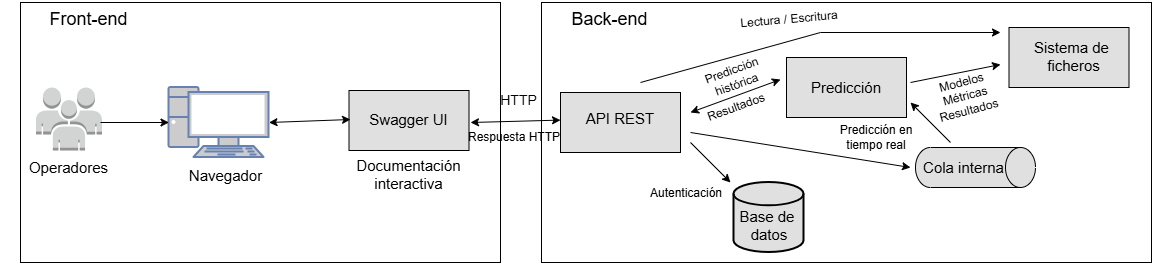
\includegraphics[width=1\textwidth]{imagenes/arquitectura_sistema.png}
\caption{Arquitectura del sistema.}
\label{fig:arquitectura_sistema}
\end{figure}


\section{Diseño de la base de datos}

Se crea una base de datos donde se guarda toda la información de los usuarios para controlar su acceso en el sistema. Esta información se almacena en una base de datos relacional, a diferencia de otras partes del proyecto como modelos entrenados, métricas experimentales o resultados de predicción que se guardan en el sistema de ficheros. Esto permite separar la gestión de usuarios del código de nuestra aplicación y evita tener credenciales escritas en los ficheros del proyecto. De este modo el sistema queda más seguro, manejable y preparado para futuras ampliaciones.

La base de datos solo dispone de una tabla, la cual se llama \emph{usuarios}. Esta guarda la información que precisa el sistema para autenticar a los usuarios y controlar sus permisos de acceso. Además, no se almacenan las predicciones generadas por los modelos en la base de datos, ya que estas se guardan en ficheros JSON separados por usuario y tipo de predicción. Esto resulta suficiente para el alcance actual del sistema y evita sobrecargar la base de datos con grandes volúmenes de predicciones individuales. Esta estructura en el diseño permite una futura ampliación en la que los resultados puedan almacenarse también en tablas relacionales, permitiendo consultas históricas, auditoría y análisis más avanzados. En la Figura~\ref{fig:diseno_bd} se muestra el diseño de la base de datos utilizada por el sistema.

\begin{figure}[H]
\centering
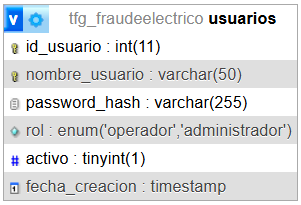
\includegraphics[width=0.75\textwidth]{imagenes/diseno_bd.png}
\caption{Diseño de la Base de Datos.}
\label{fig:diseno_bd}
\end{figure}


\subsection{Tabla usuarios}

Esta tabla está formada por varios elementos como un identificador único, un nombre de usuario, una contraseña almacenada mediante hash, un rol dentro del sistema, un estado de activación y una fecha de creación. El uso de contraseñas cifradas mediante hash evita tener contraseñas en texto plano, así se consigue reducir los casos de accesos no autorizados. El campo de estado permite desactivar usuarios sin necesidad de eliminarlos físicamente, conservando así la integridad de la información. En la Figura~\ref{fig:tabla_usuarios} se muestran sus atributos junto con detalles como el tipo de dato.

\begin{figure}[H]
\centering
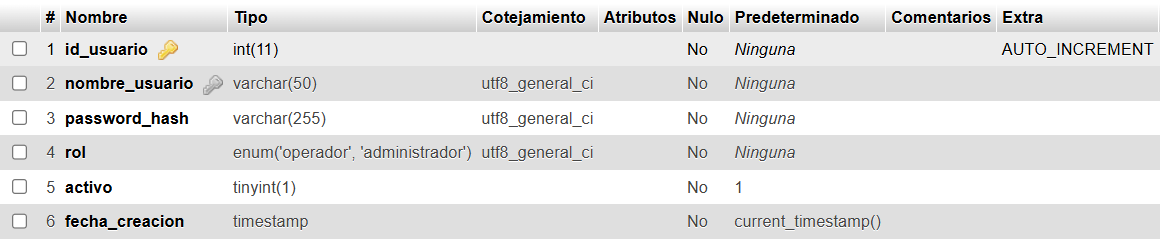
\includegraphics[width=1\textwidth]{imagenes/tabla_usuarios.png}
\caption{Diseño de la tabla de usuarios.}
\label{fig:tabla_usuarios}
\end{figure}


\section{Diseño del almacenamiento de ficheros}

El sistema guarda en disco los recursos creados durante la fase experimental y los resultados producidos durante el uso de la aplicación. Con esta división se reserva la base de datos para información relacionada a los usuarios, mientras que el sistema de ficheros se utiliza para almacenar recursos más pesados o generados externamente, como modelos entrenados, gráficas, métricas y resultados de predicción. Esta decisión se debe a que algunos elementos del sistema no encajan de forma natural en una tabla relacional. Los modelos entrenados, los escaladores, las listas de columnas esperadas, las curvas ROC, los ficheros de métricas y la importancia de variables son recursos producidos durante la fase experimental y posteriormente reutilizados por la aplicación. Se almacenan como ficheros dentro de la estructura del proyecto, permitiendo que la \emph{API} los cargue cuando sean necesarios sin repetir el entrenamiento de los modelos.

La carpeta \emph{models/} se utiliza para guardar los recursos necesarios para realizar las predicciones. En ella se encuentran los modelos entrenados, las columnas esperadas por cada modelo y, en el caso del modelo online, el escalador utilizado durante la fase experimental. Estos garantizan que los datos importados por el operador se procesen con la misma estructura y condiciones que los datos utilizados durante el entrenamiento. Por otro lado, la carpeta \emph{results/} almacena los resultados experimentales y los recursos complementarios asociados a los modelos. En esta carpeta se encuentran las métricas de evaluación, las curvas ROC, la importancia de variables de \emph{XGBoost} y los resultados. De esta forma, la aplicación puede mostrar información complementaria sin recalcularla en cada consulta. Los resultados de las predicciones se guardan separados por usuario y por tipo de predicción. Así se evita que los resultados de distintos operadores se mezclen y permite distinguir entre la última predicción histórica y la última predicción en tiempo real.

Los archivos en el entorno local se guardan directamente en el sistema de ficheros del ordenador donde la aplicación está funcionando. Estos pueden estar en el disco persistente vinculado al servidor, como un volumen \emph{EBS}, por ejemplo, cuando se despliega en un servidor sobre una instancia de \emph{AWS EC2}. Así, los modelos, resultados y recursos adicionales continúan accesibles incluso si se vuelve a iniciar la aplicación. El almacenamiento de los ficheros podría trasladarse a un servicio externo como \emph{Amazon S3} para una versión más segura con requerimientos más altos de mantenimiento, disponibilidad y escalabilidad. Esto posibilita la separación de los archivos de la instancia de ejecución, el mejoramiento de la persistencia y la administración más sólida de los recursos que produce el sistema, así como también hacer copias de seguridad más fácilmente.


\section{Diseño de la API REST}

En esta sección se puede visualizar el diseño del sistema, tanto en su versión inicial como estaba planeado el sistema, como en su versión final ya implementado y funcional.


\subsection{Bocetos iniciales}

Antes de realizar la implementación y diseño final del sistema se realiza unos bocetos iniciales para plasmar la idea inicial del sistema. Estos bocetos están realizados a través de un software especializado llamado \emph{balsamiq} y muestran cada una de las ventanas y funcionalidades del sistema. En la Figura~\ref{fig:main_boceto} se puede ver la ventana principal del sistema.

\begin{figure}[H]
\centering
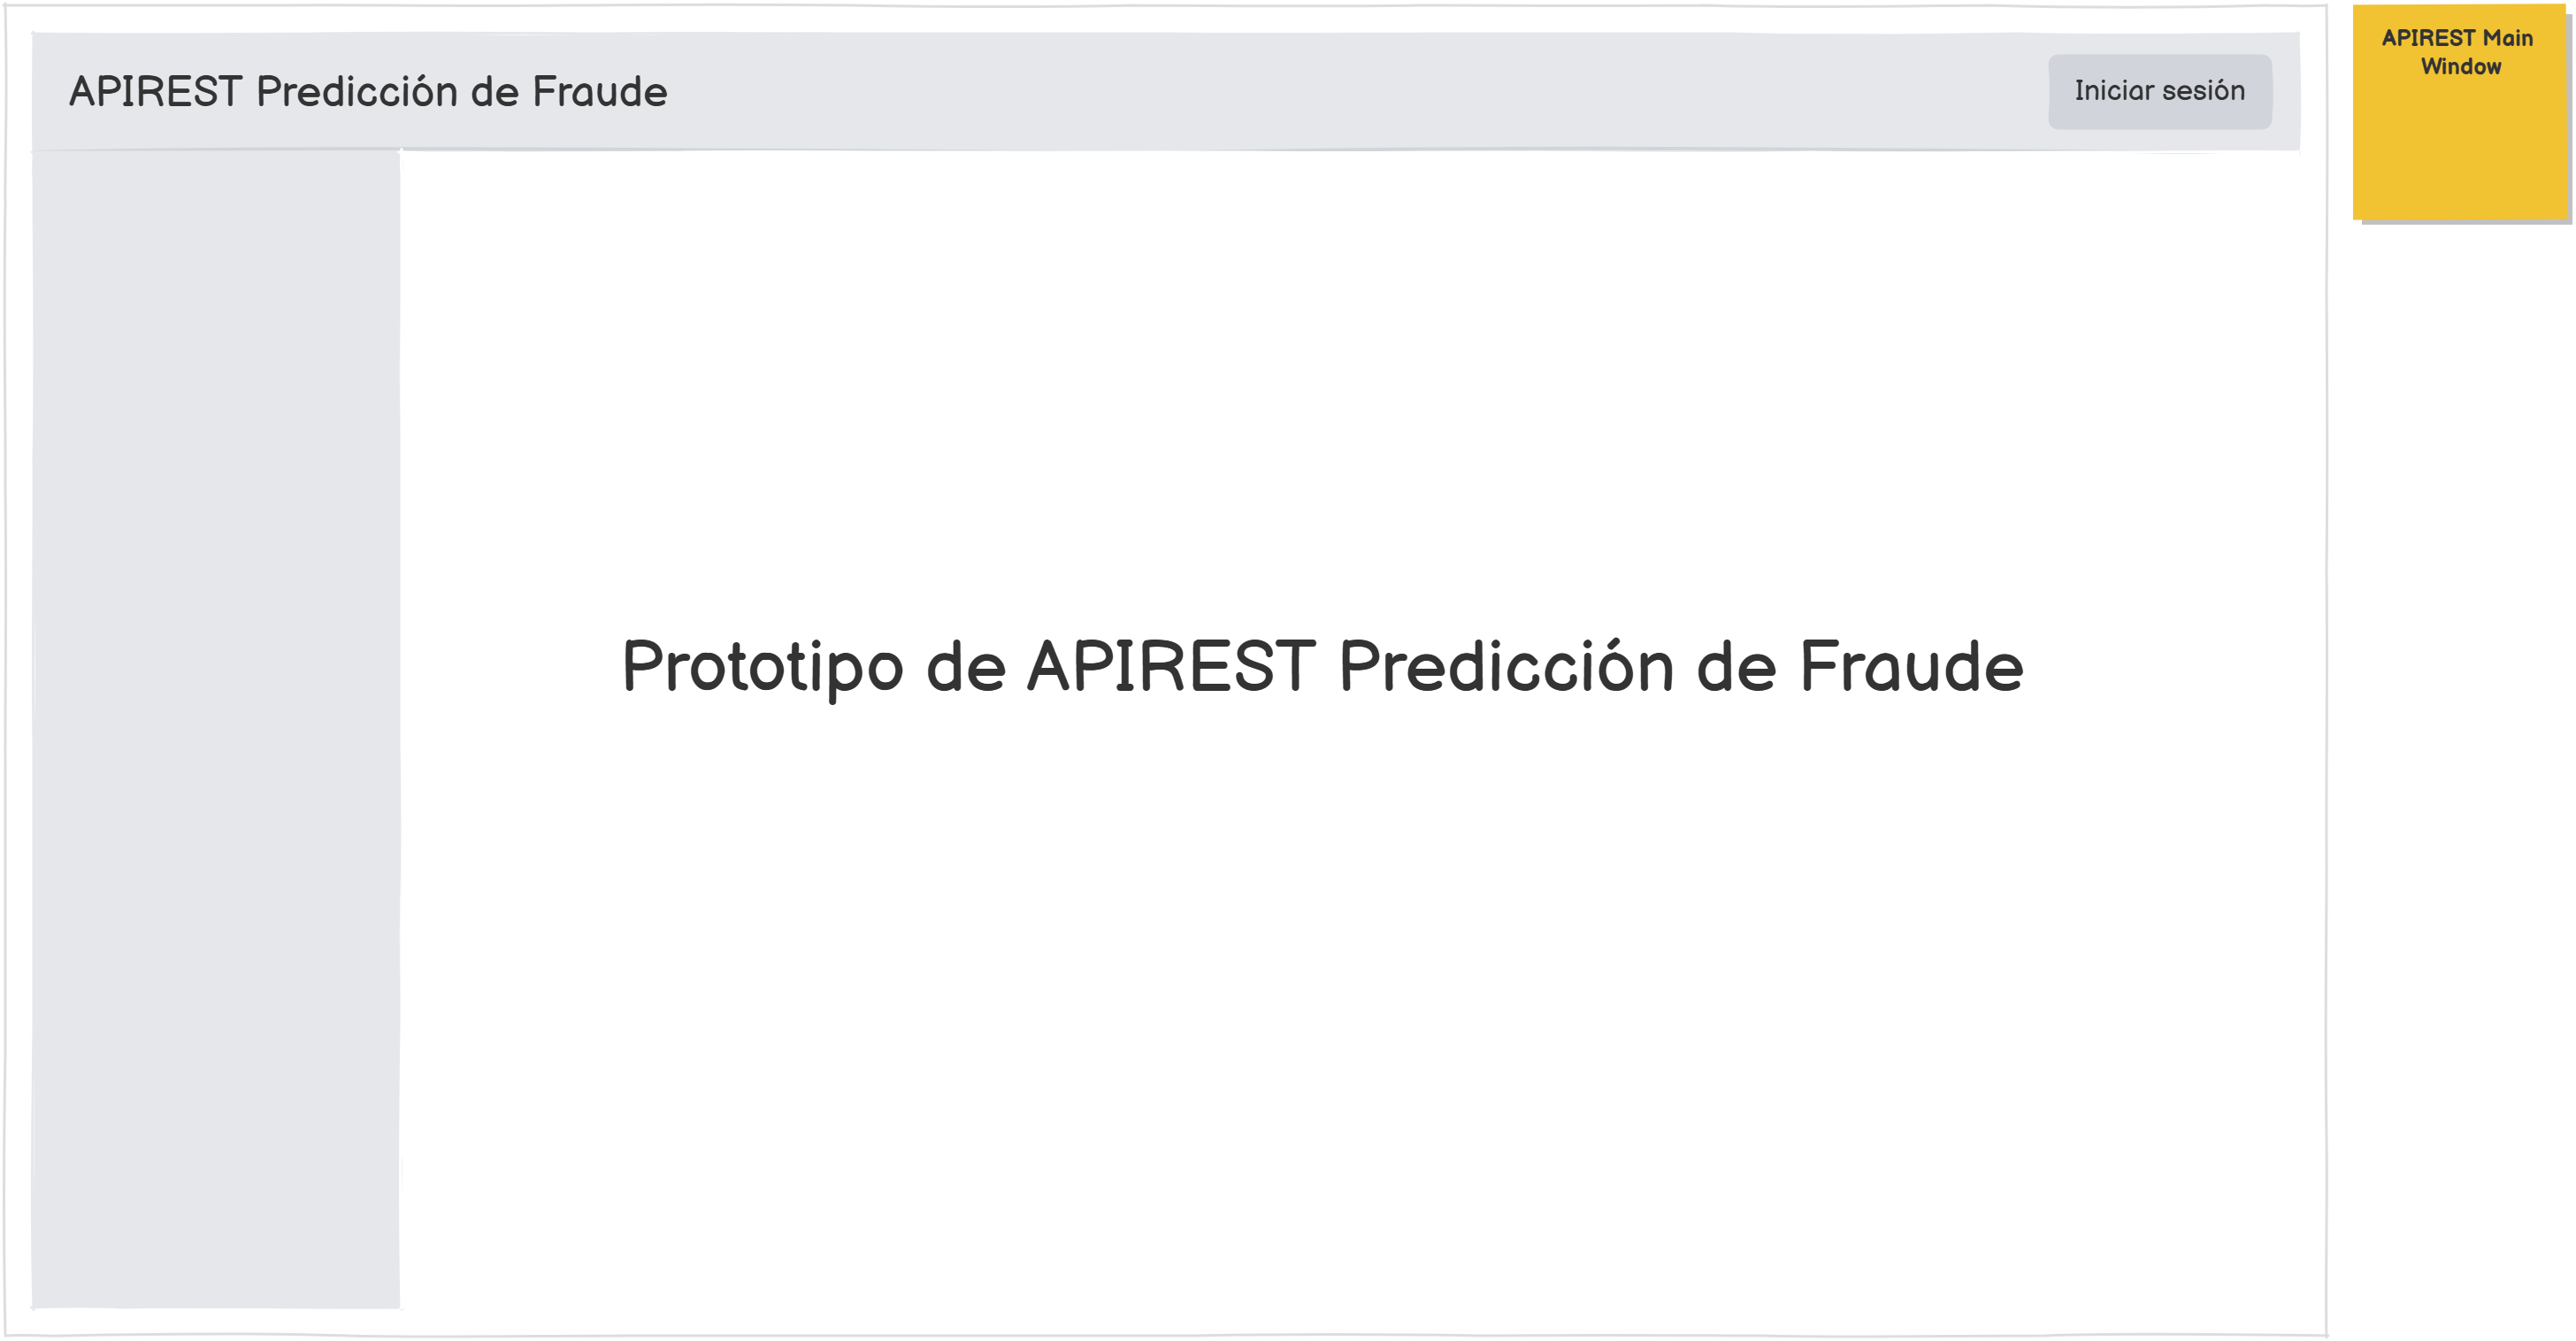
\includegraphics[width=1\textwidth]{imagenes/main_boceto.png}
\caption{Boceto de la ventana principal del sistema.}
\label{fig:main_boceto}
\end{figure}


\subsubsection{Ventanas de autenticación}

Se muestran las ventanas que pertenecen a los casos de uso de Iniciar sesión y Cerrar sesión, relacionados con la autenticación en el sistema.

\begin{figure}[H]
\centering
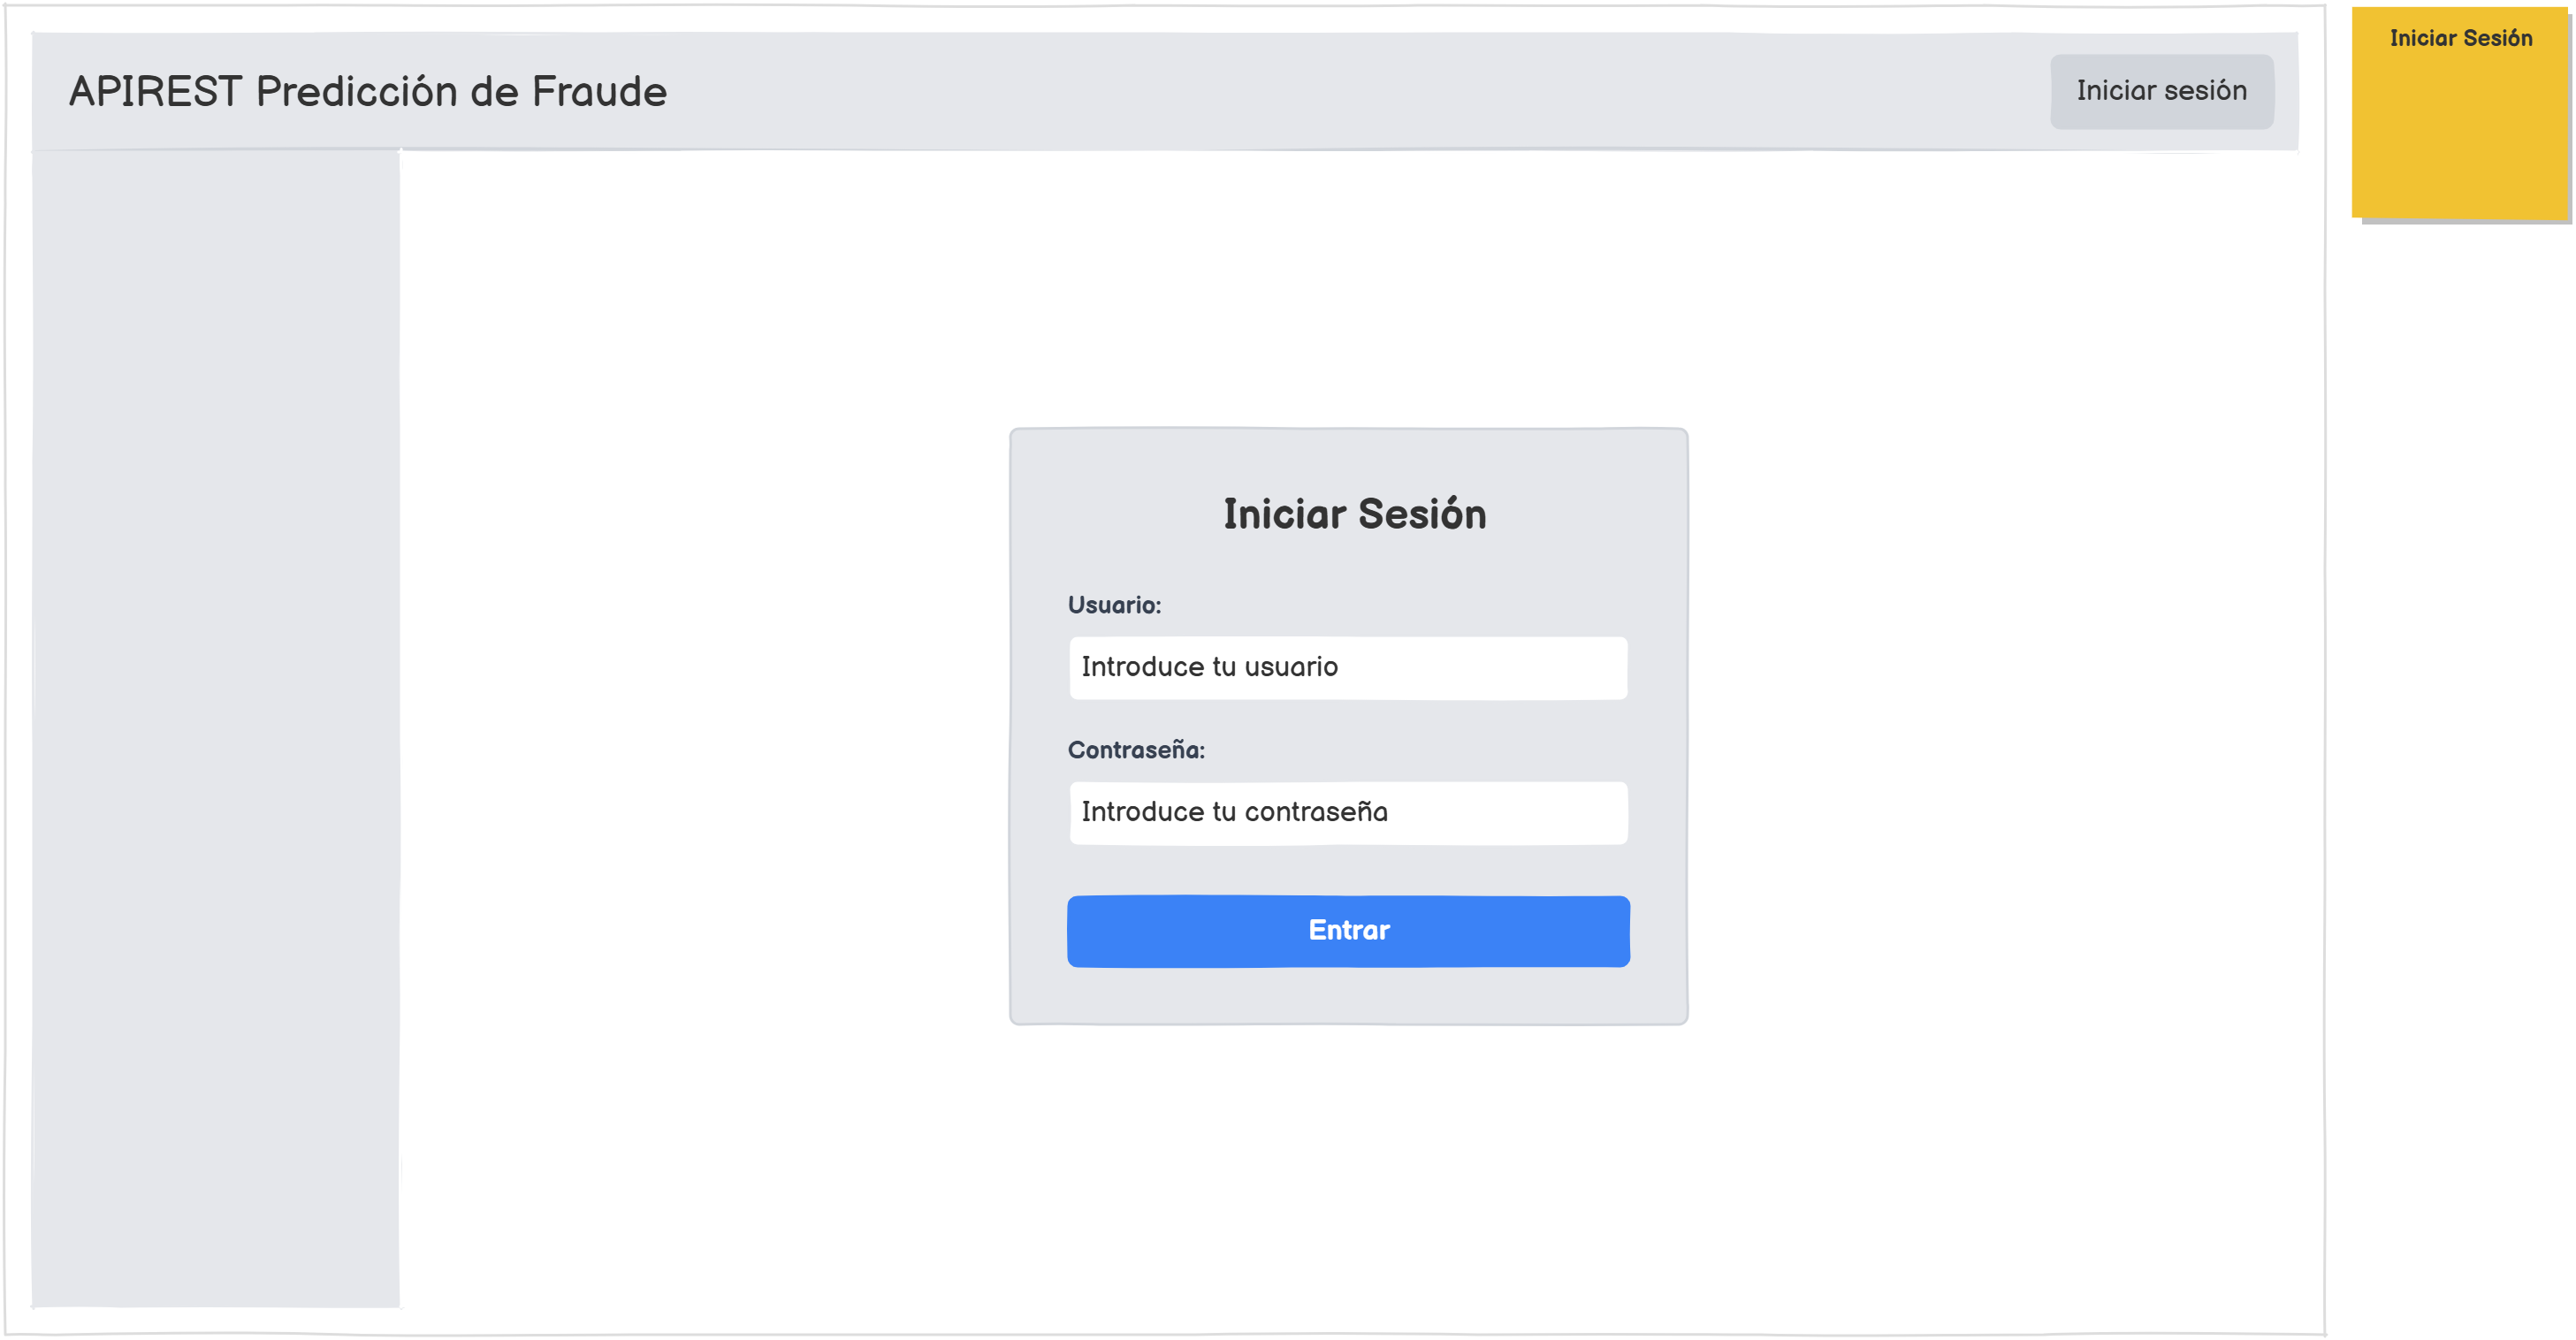
\includegraphics[width=1\textwidth]{imagenes/iniciarSesion_boceto.png}
\caption{Boceto de la ventana de iniciar sesión.}
\end{figure}

\begin{figure}[H]
\centering
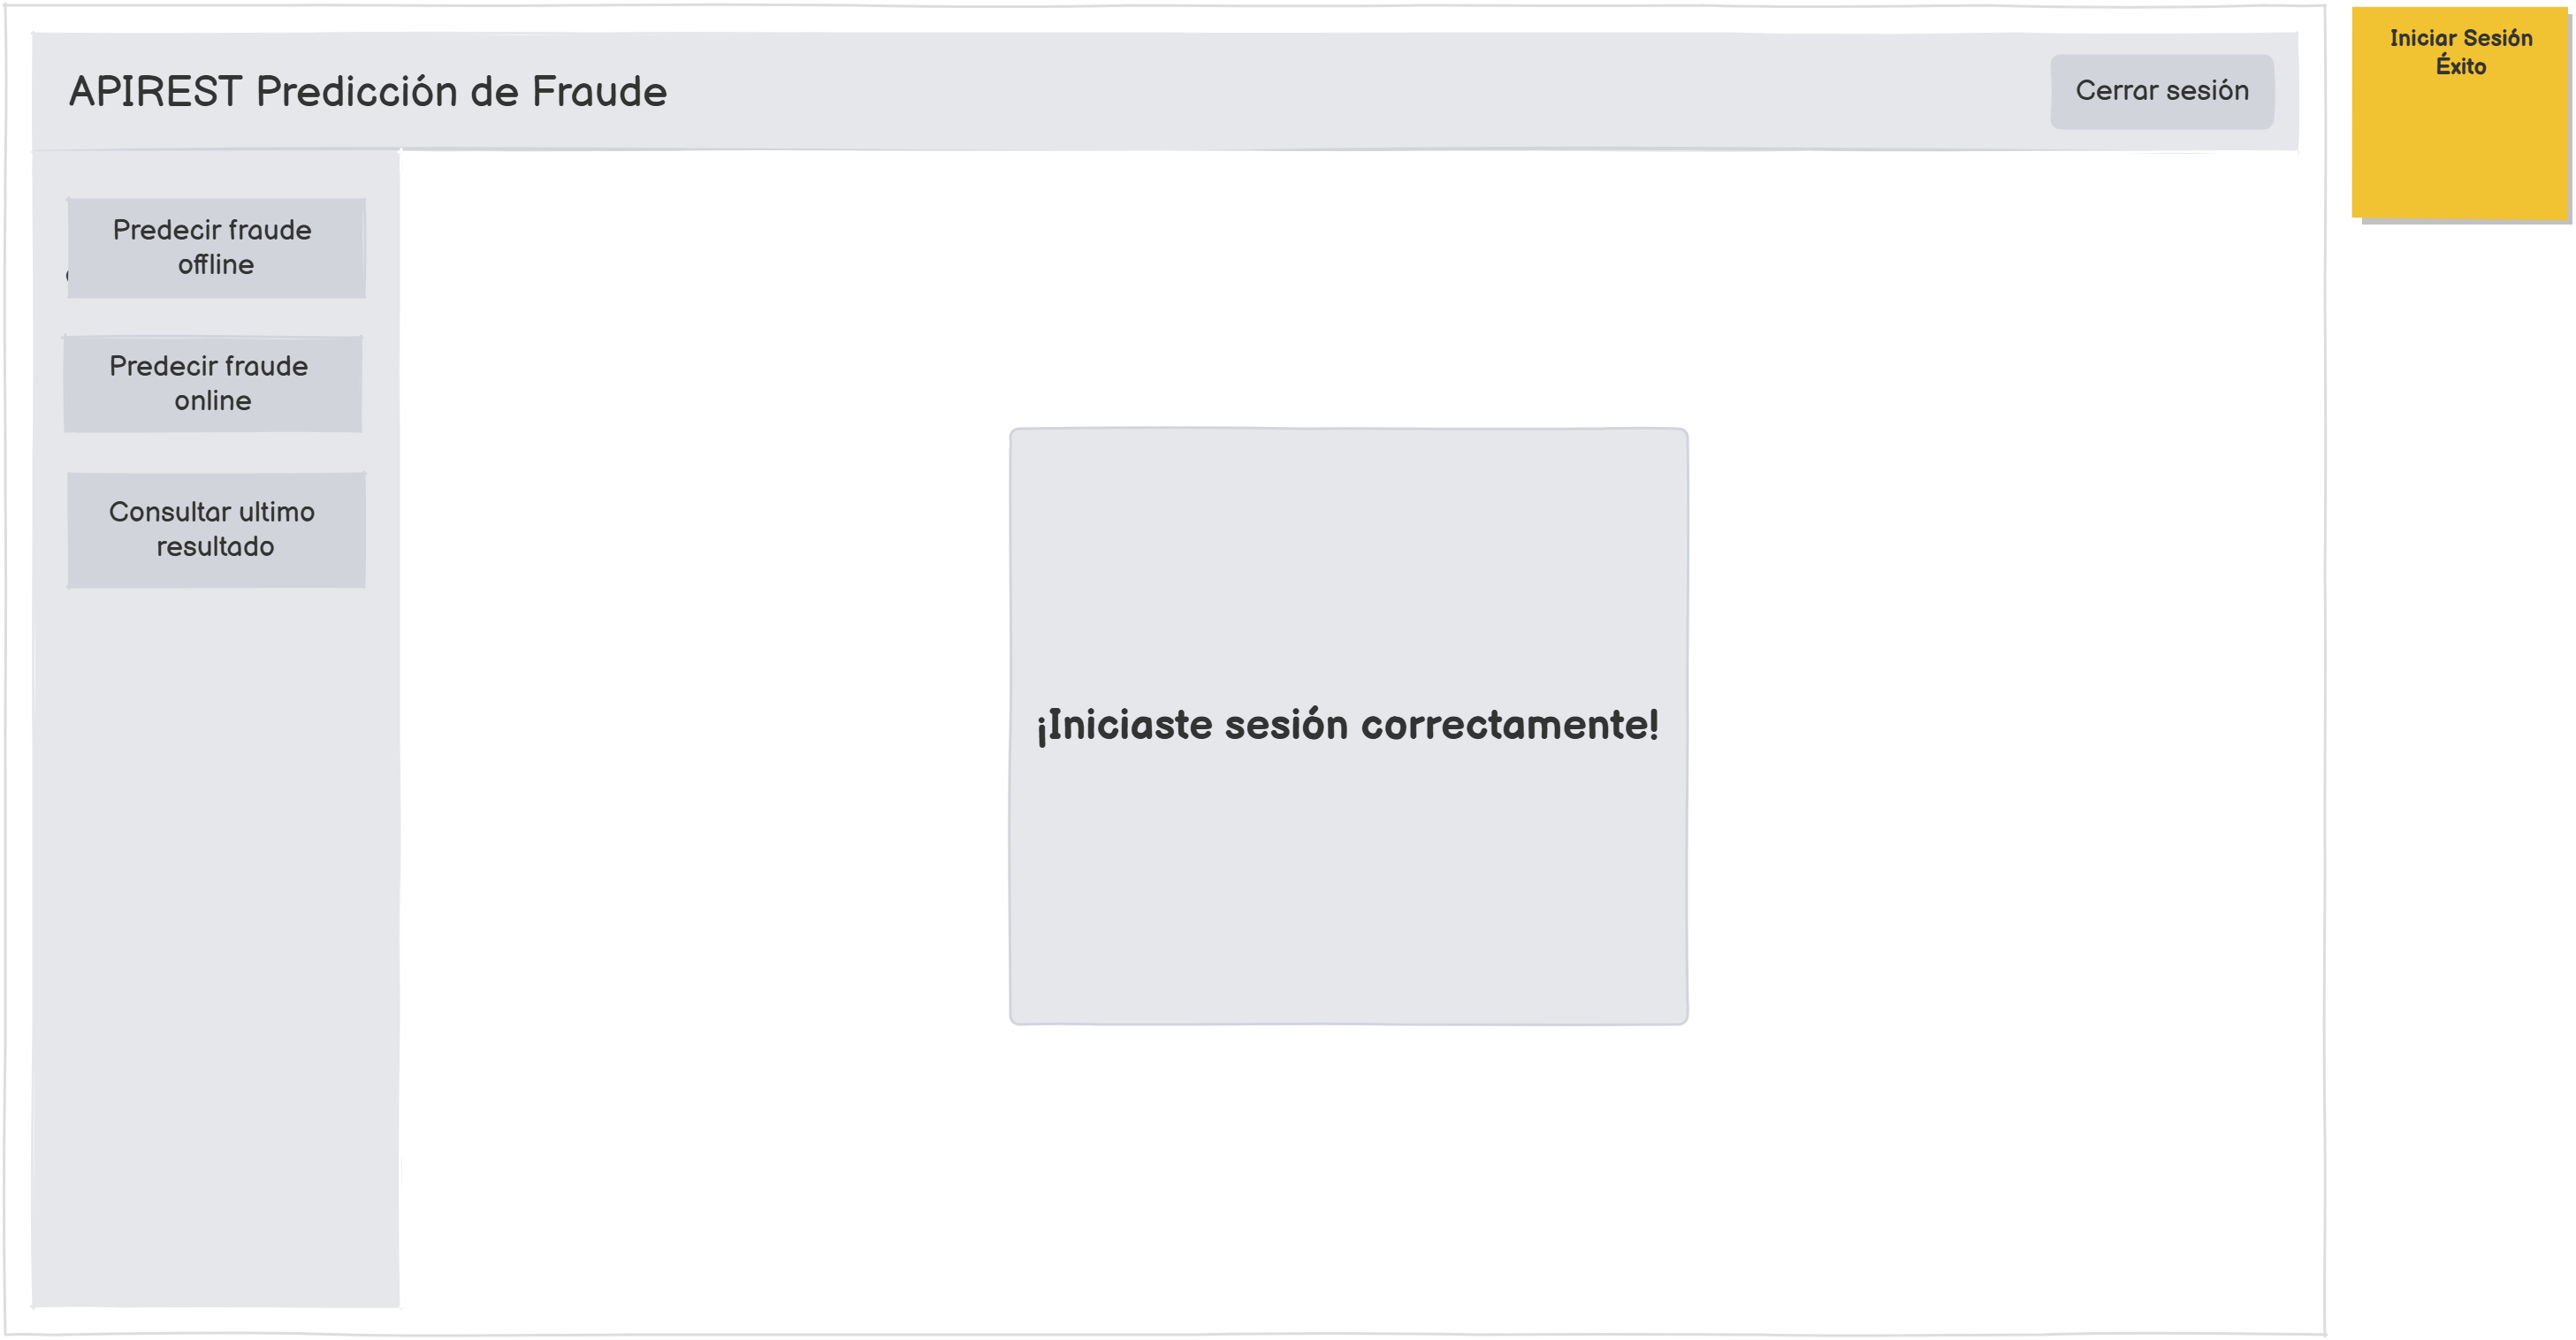
\includegraphics[width=1\textwidth]{imagenes/iniciarSesionExito_boceto.png}
\caption{Boceto de la ventana de iniciar sesión con éxito.}
\end{figure}

\begin{figure}[H]
\centering
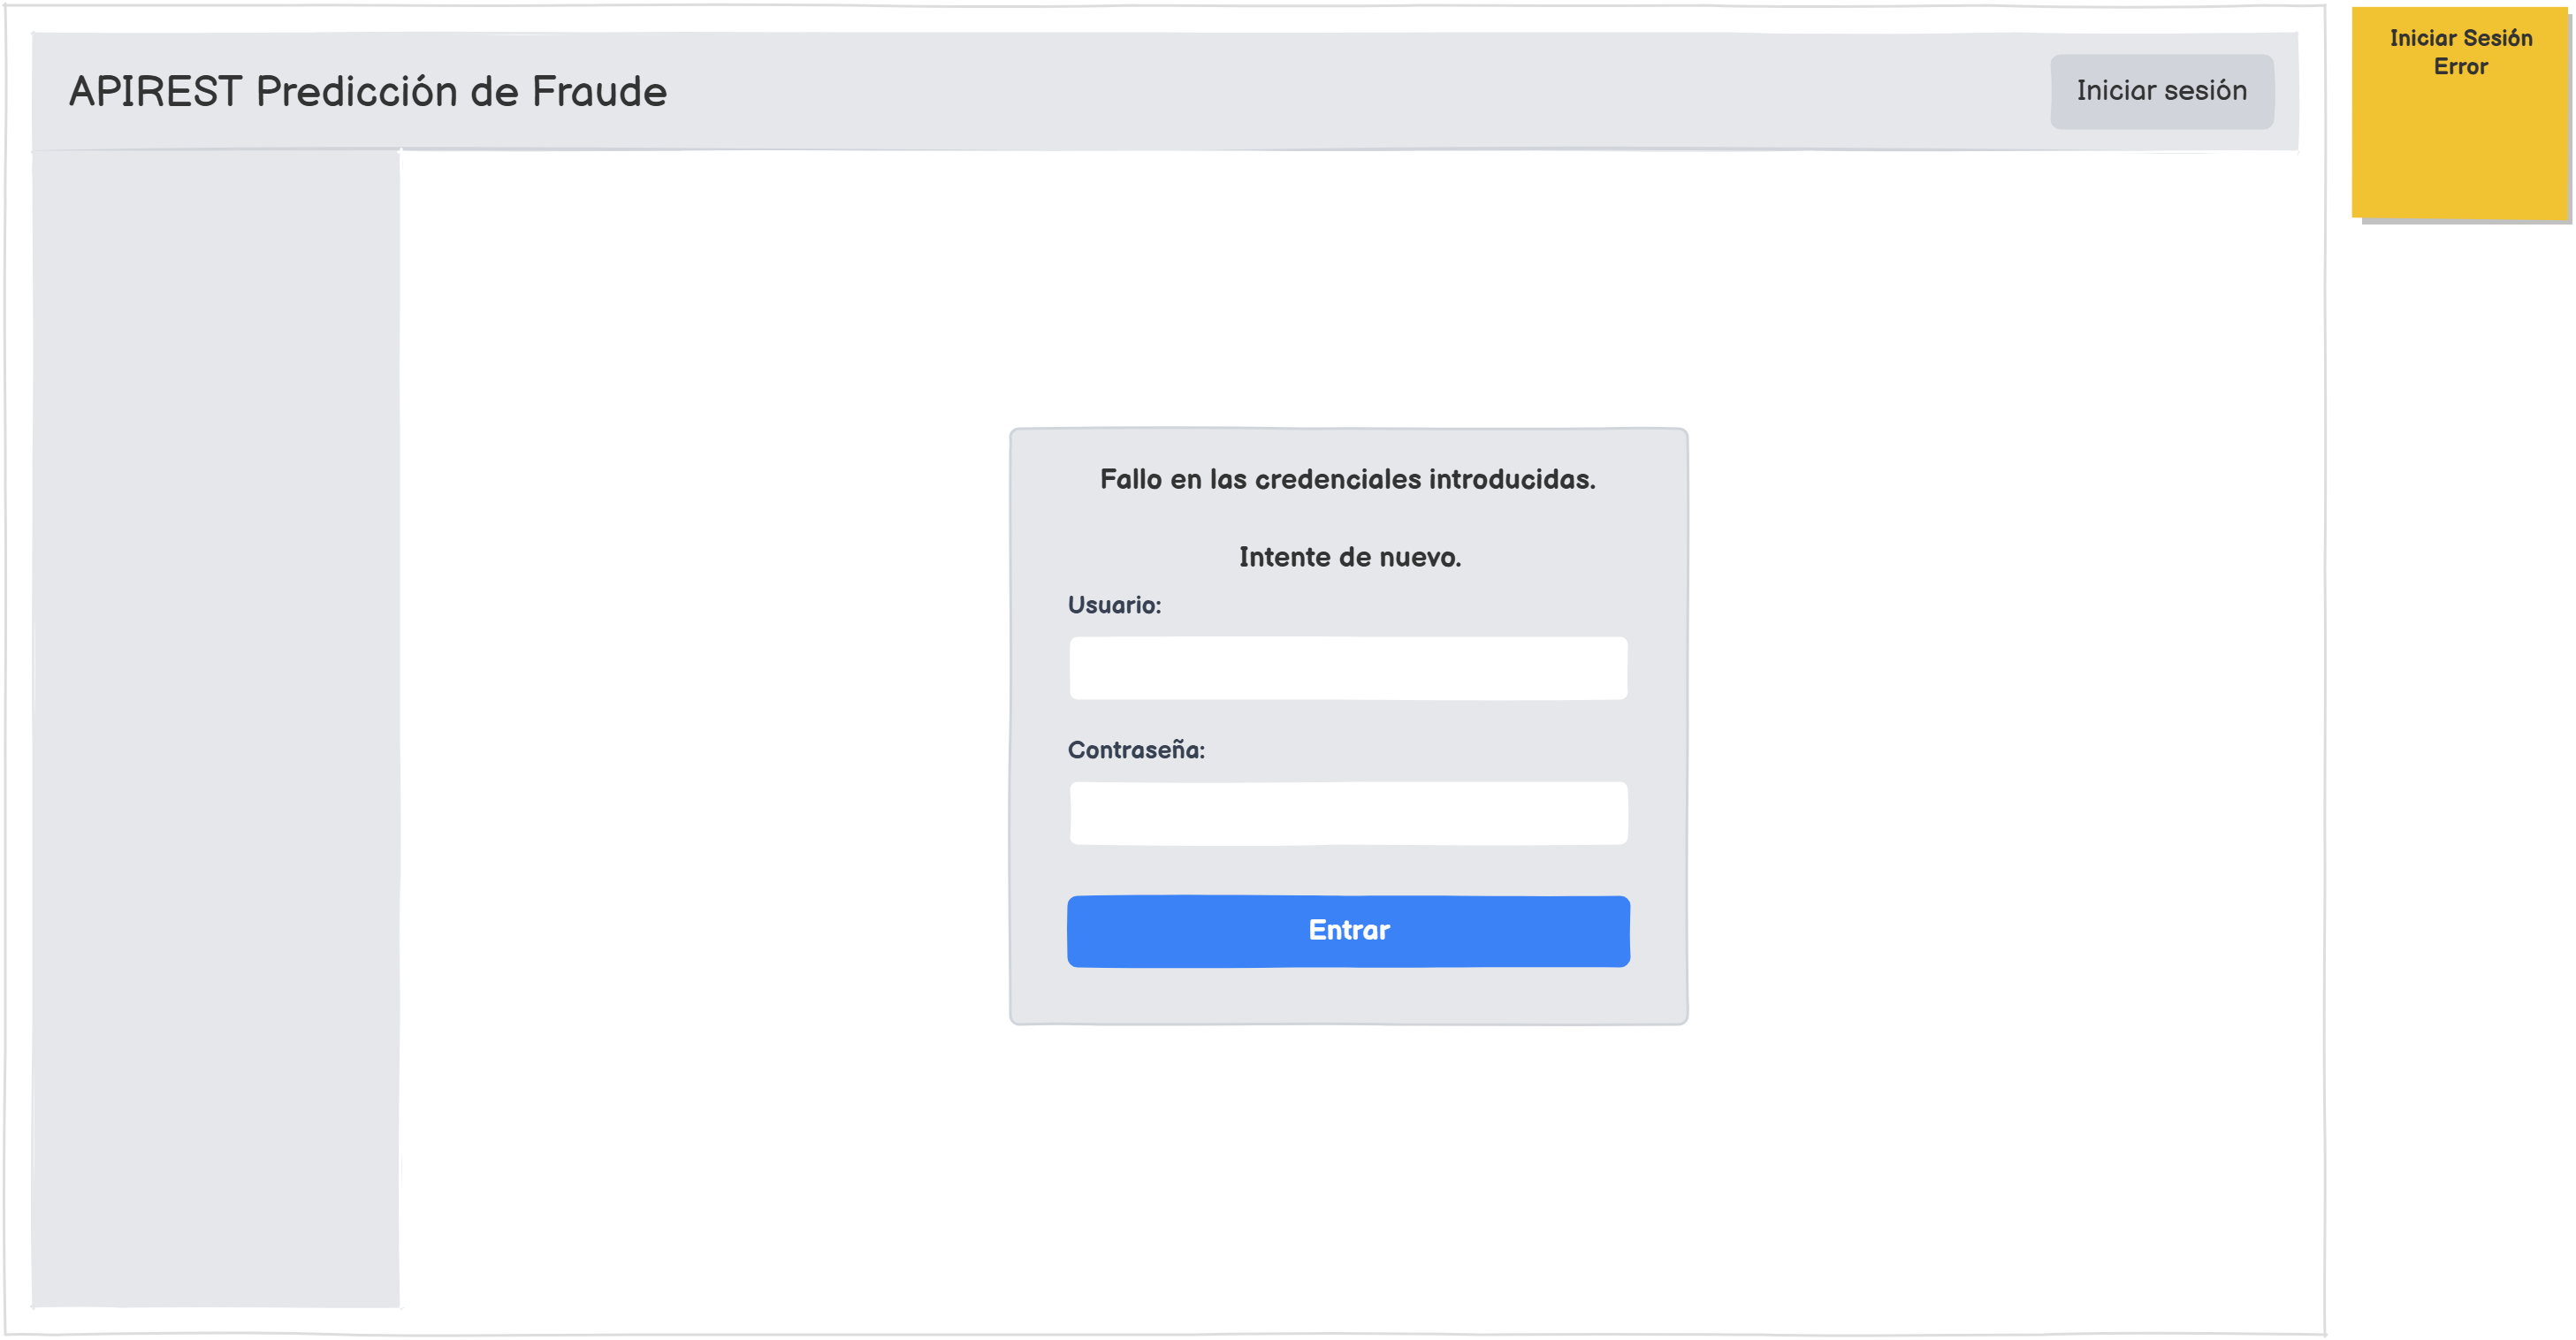
\includegraphics[width=1\textwidth]{imagenes/iniciarSesionError_boceto.png}
\caption{Boceto de la ventana de error al iniciar sesión.}
\end{figure}

\begin{figure}[H]
\centering
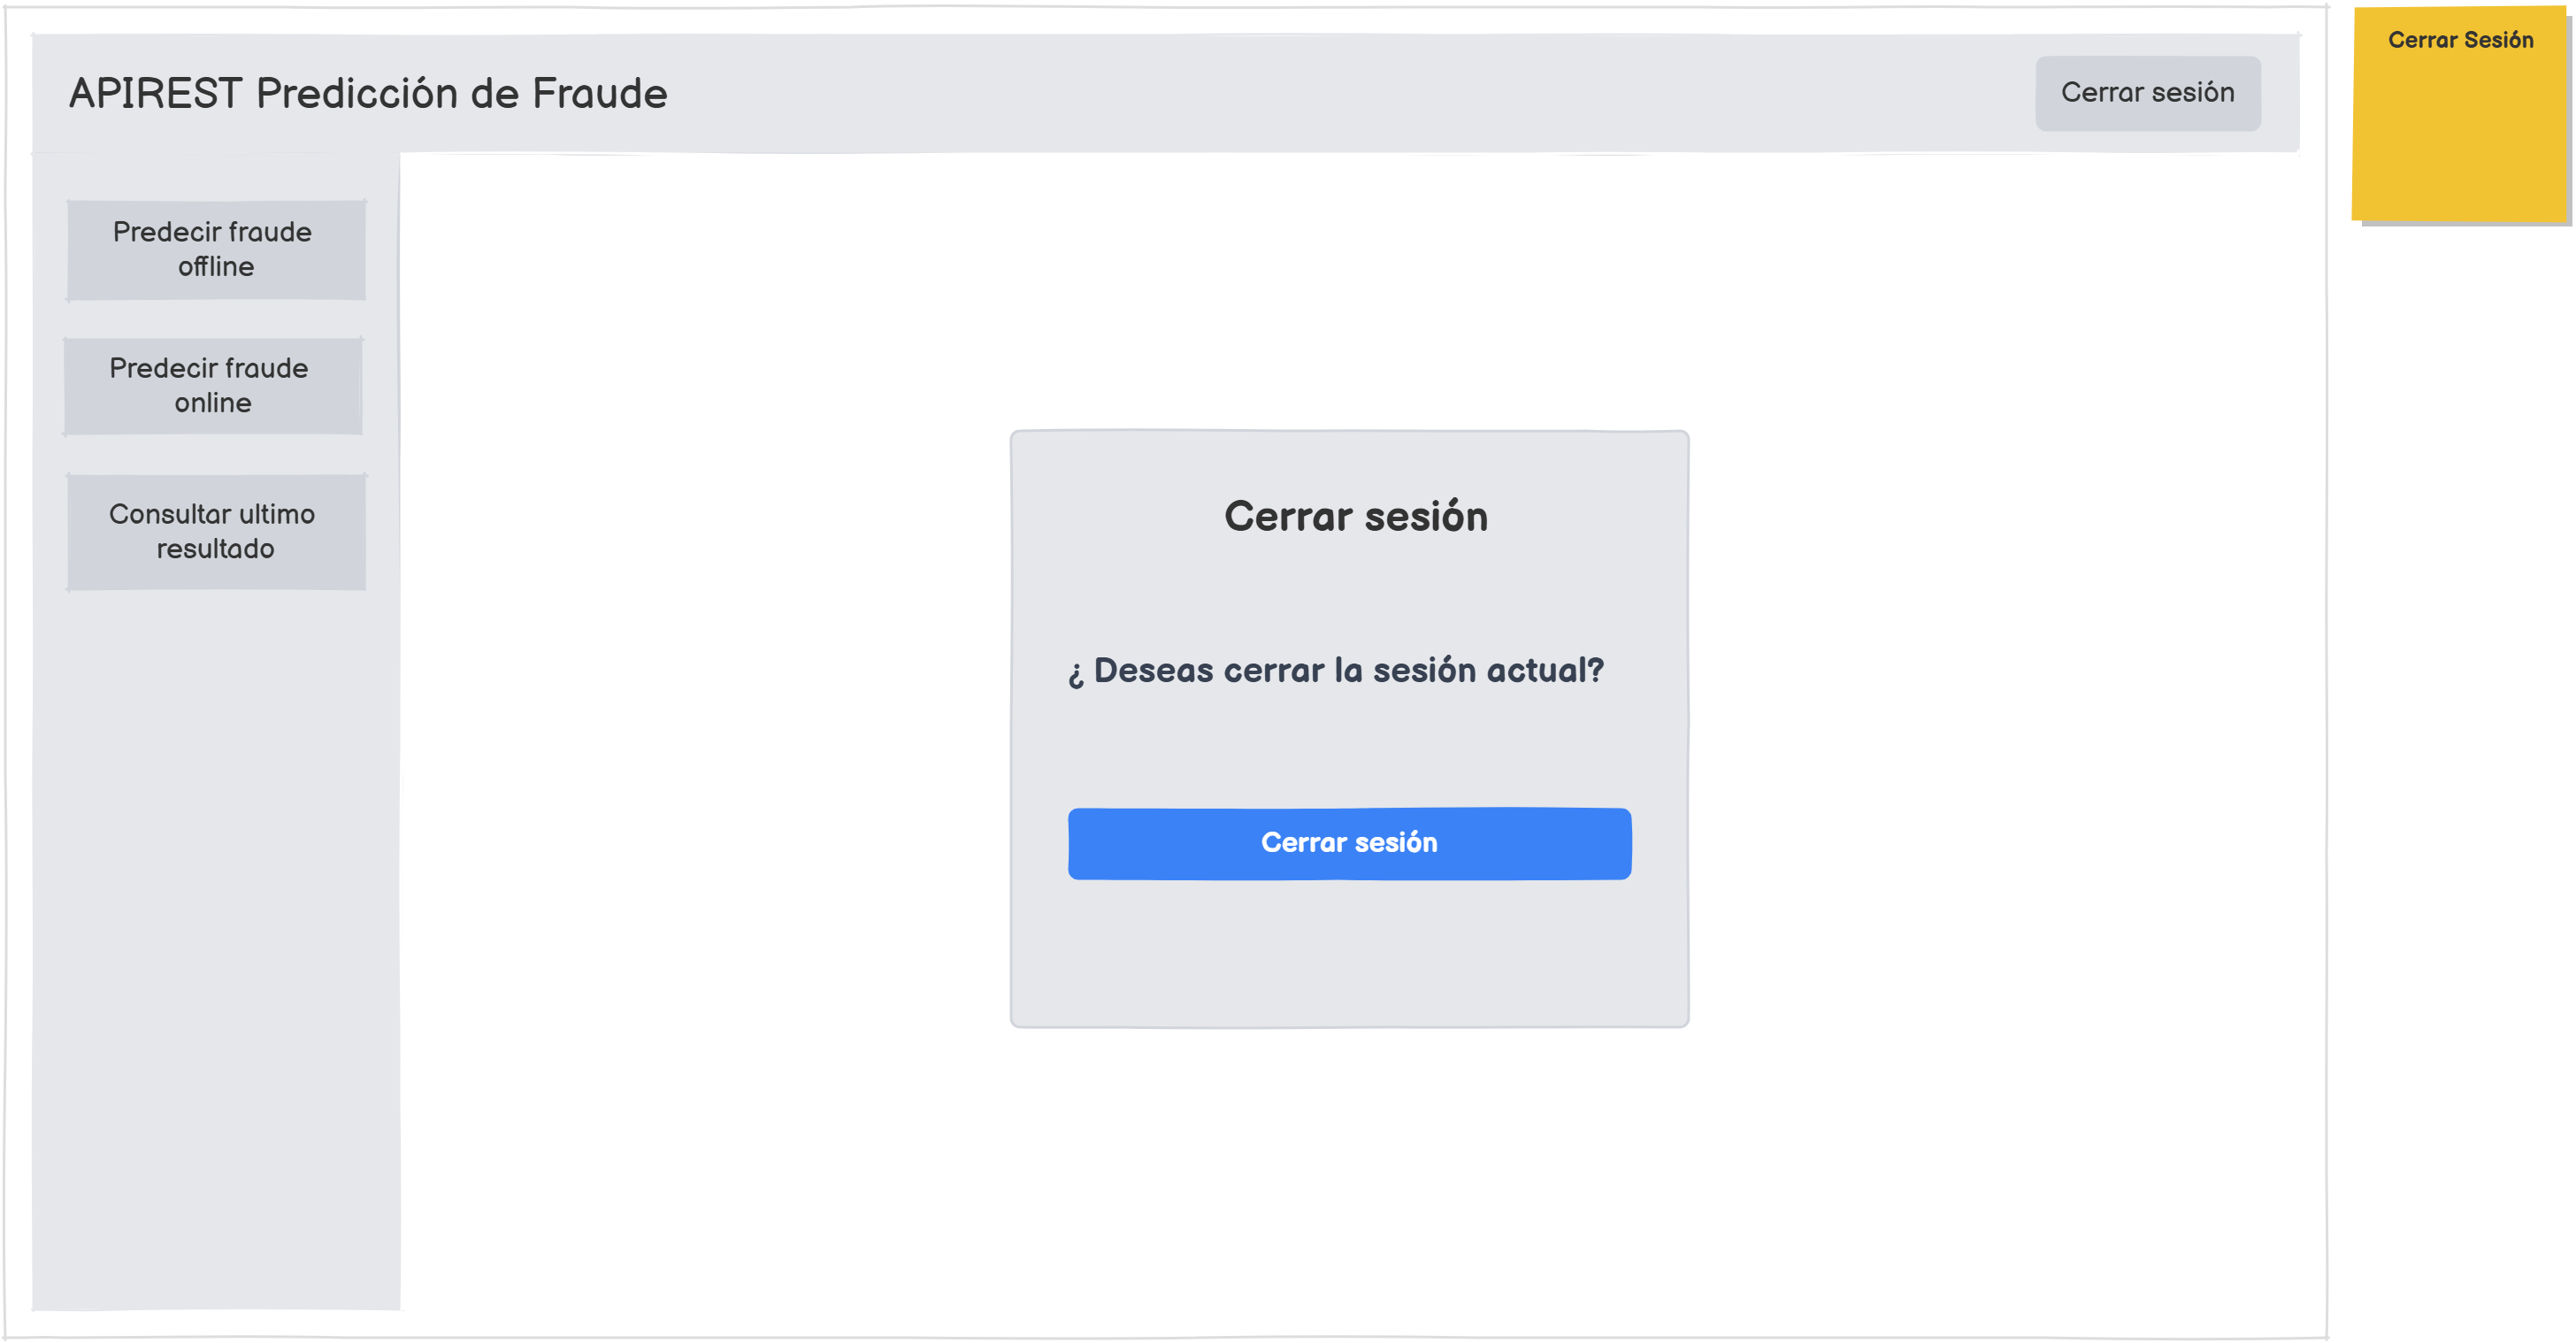
\includegraphics[width=1\textwidth]{imagenes/cerrarSesion_boceto.png}
\caption{Boceto de la ventana de cerrar sesión.}
\end{figure}

\begin{figure}[H]
\centering
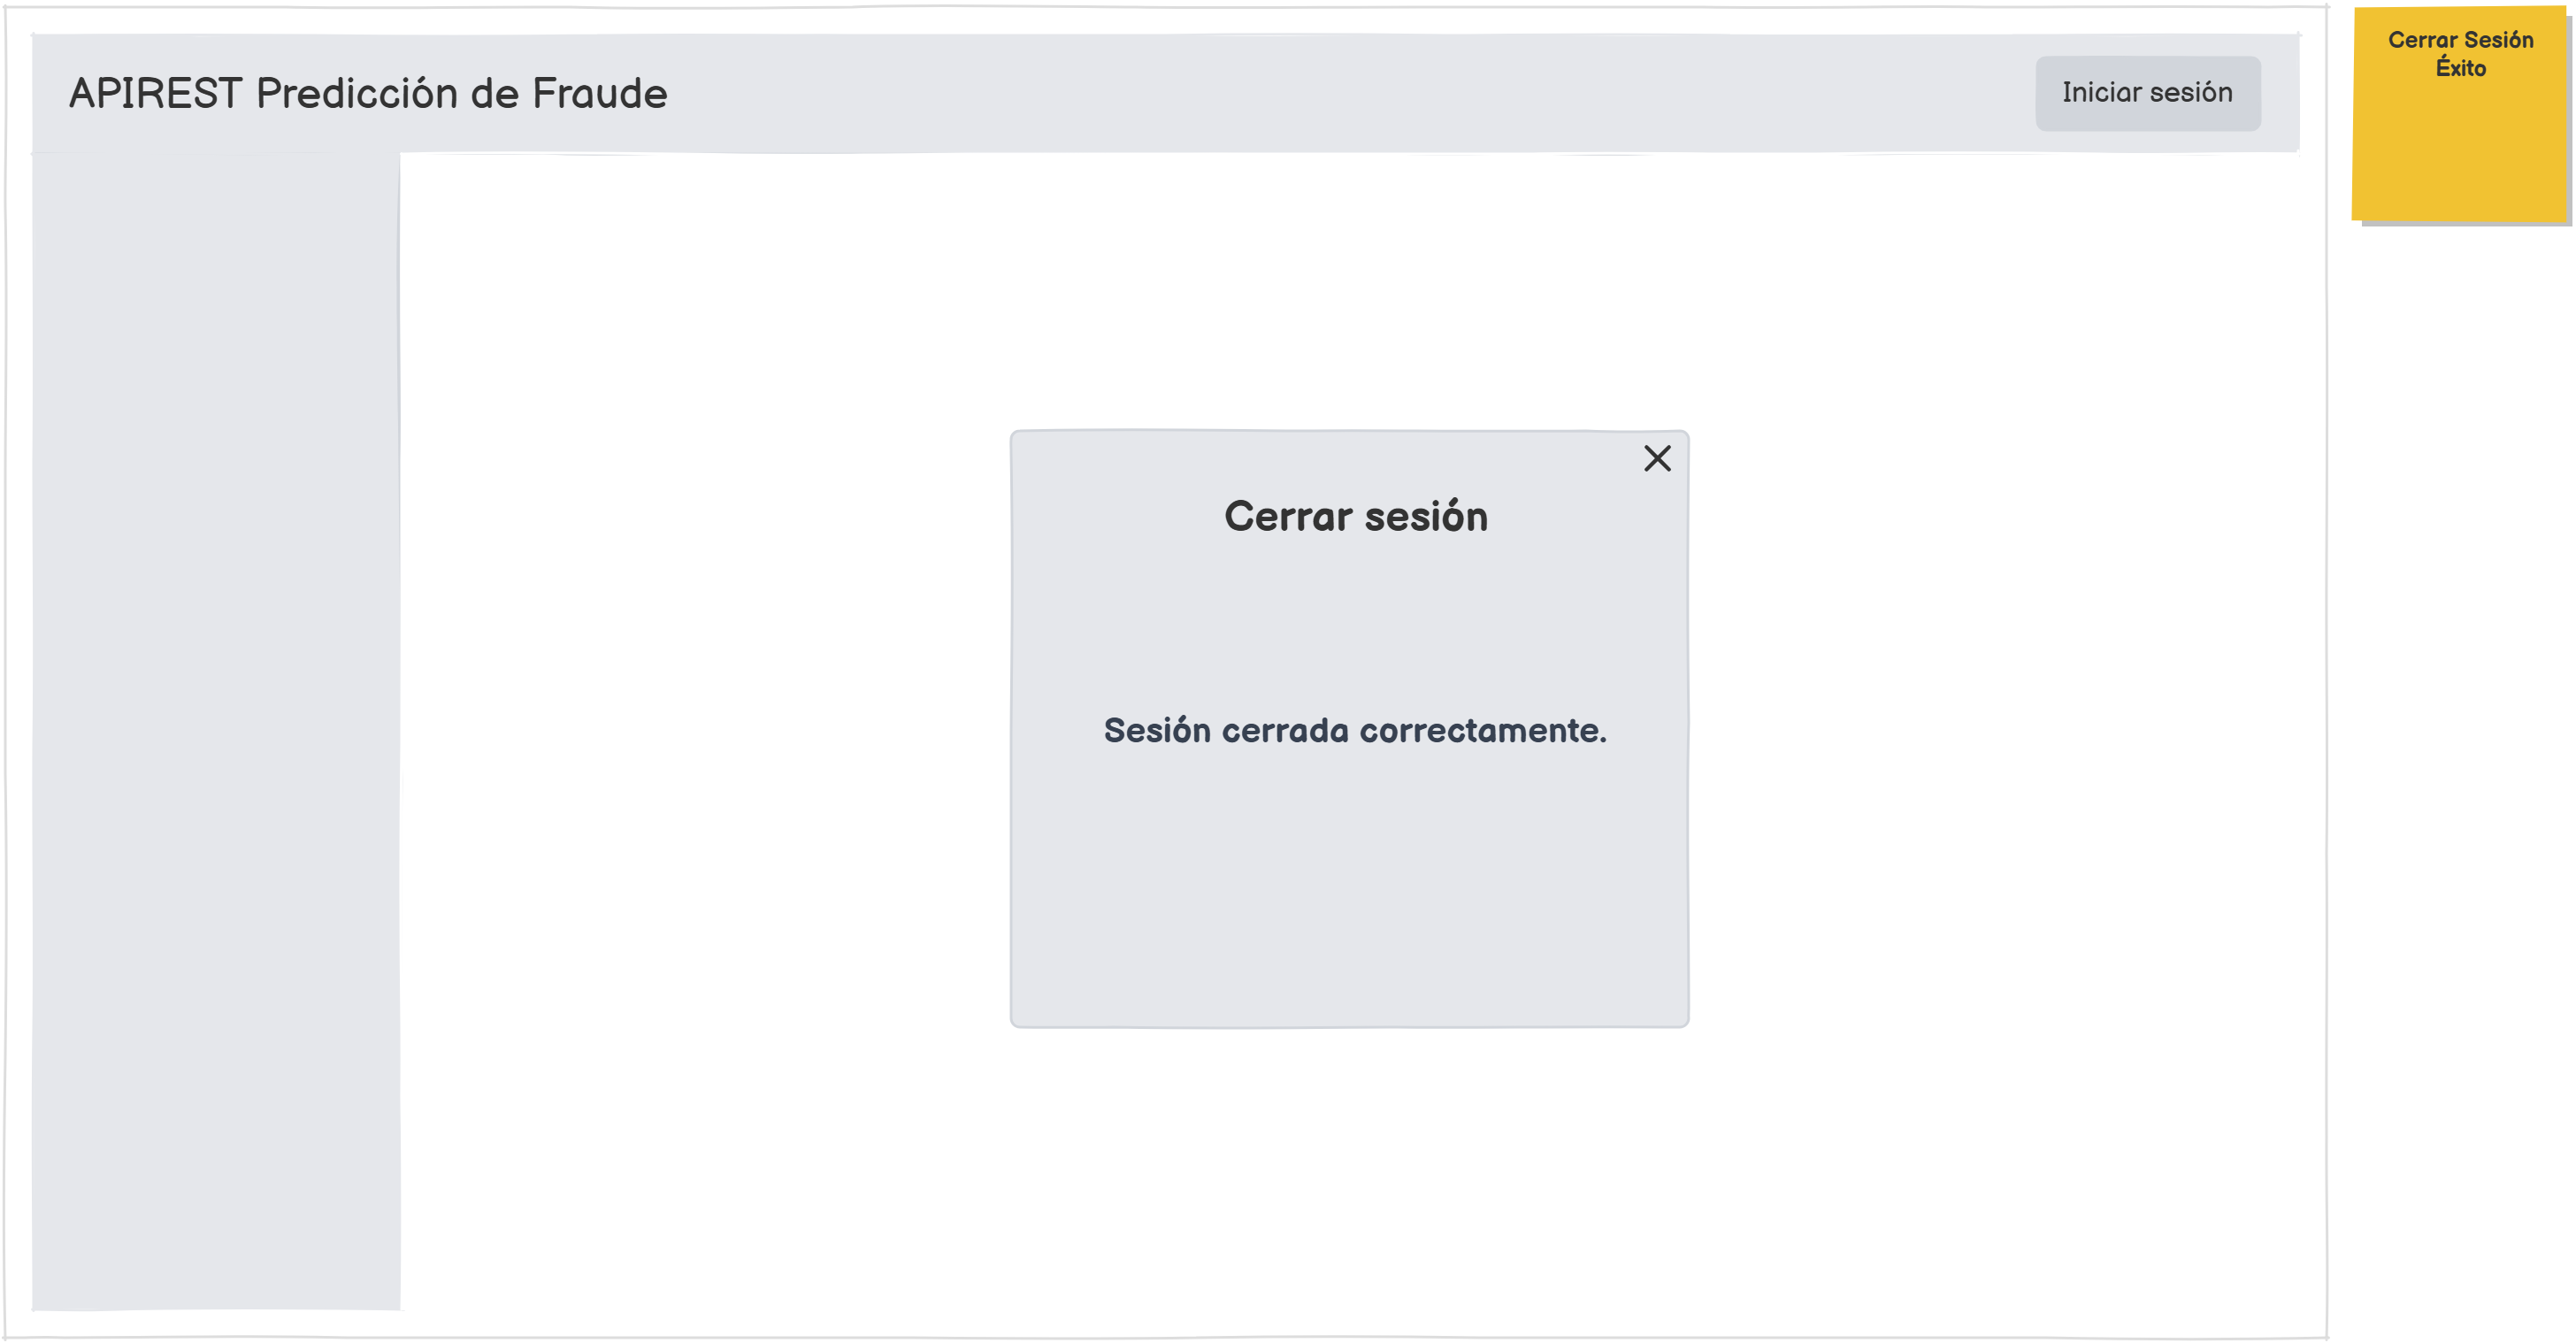
\includegraphics[width=1\textwidth]{imagenes/cerrarSesionExito_boceto.png}
\caption{Boceto de la ventana de cerrar sesión con éxito.}
\end{figure}


\subsubsection{Ventanas de predicción}
Se muestran las ventanas que pertenecen a los casos de uso de predecir fraude ya sea \emph{offline} o \emph{online} junto a posibles errores.

\begin{figure}[H]
\centering
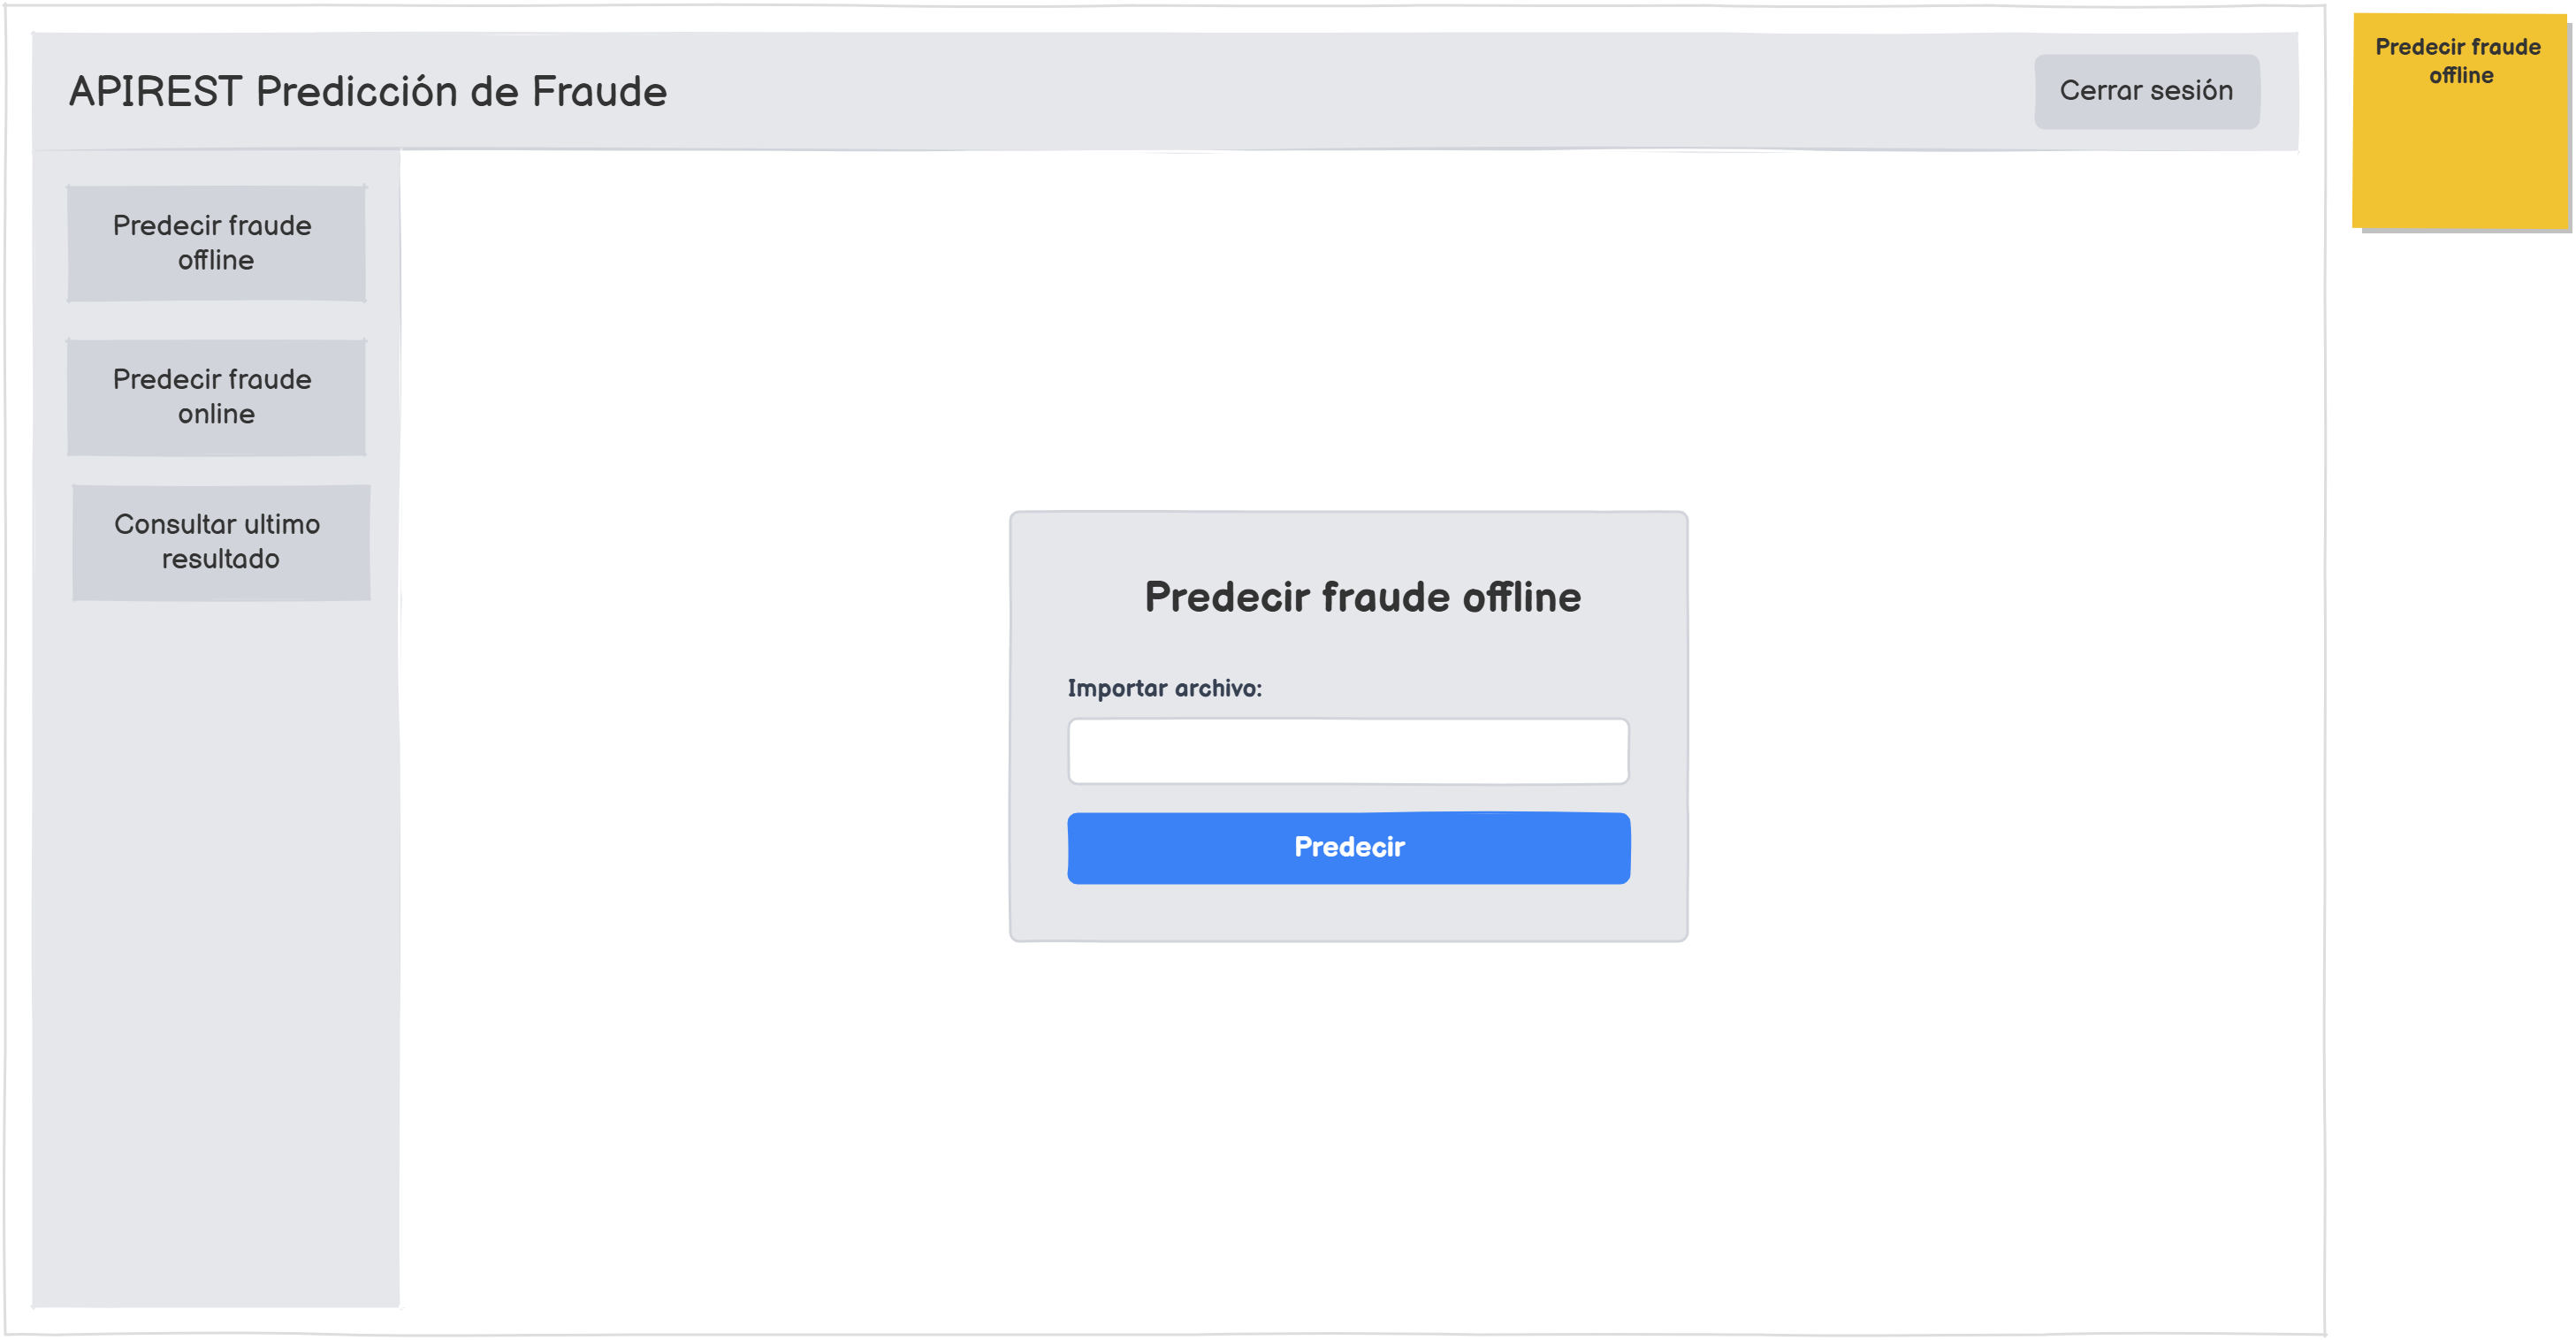
\includegraphics[width=1\textwidth]{imagenes/fraudeOffline_boceto.png}
\caption{Boceto de la ventana principal de predecir fraude \emph{offline}.}
\end{figure}

\begin{figure}[H]
\centering
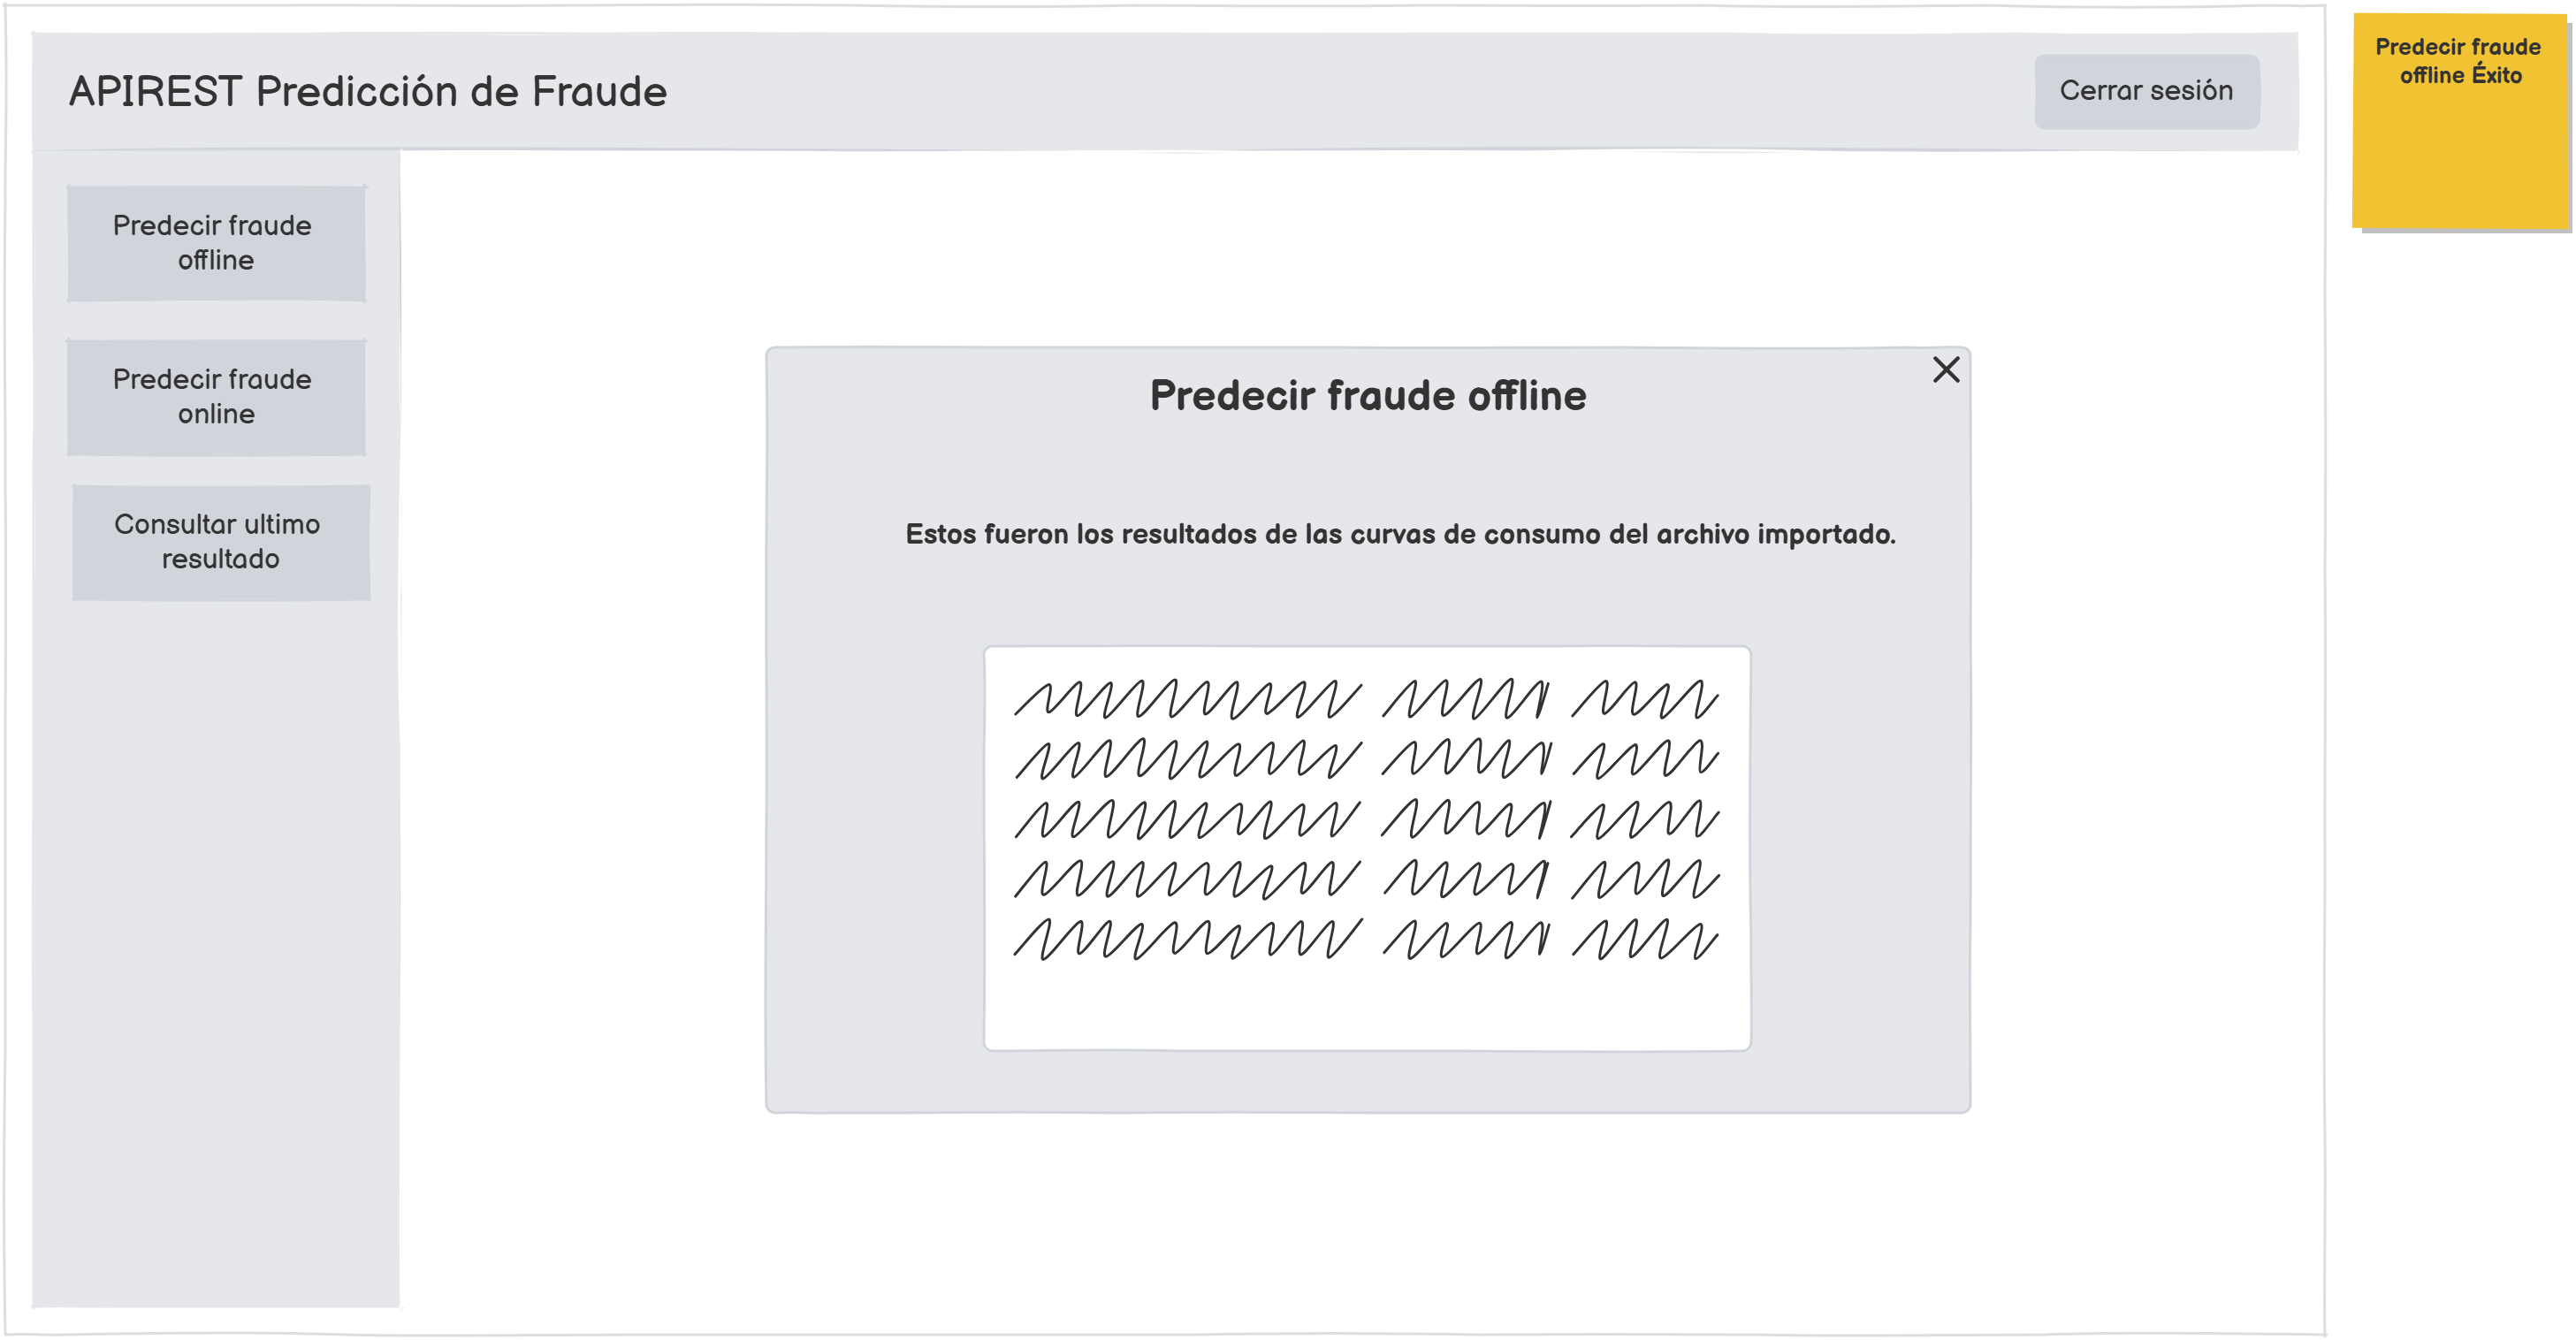
\includegraphics[width=1\textwidth]{imagenes/fraudeOfflineExito_boceto.png}
\caption{Boceto de la ventana de predecir fraude \emph{offline} con éxito.}
\end{figure}

\begin{figure}[H]
\centering
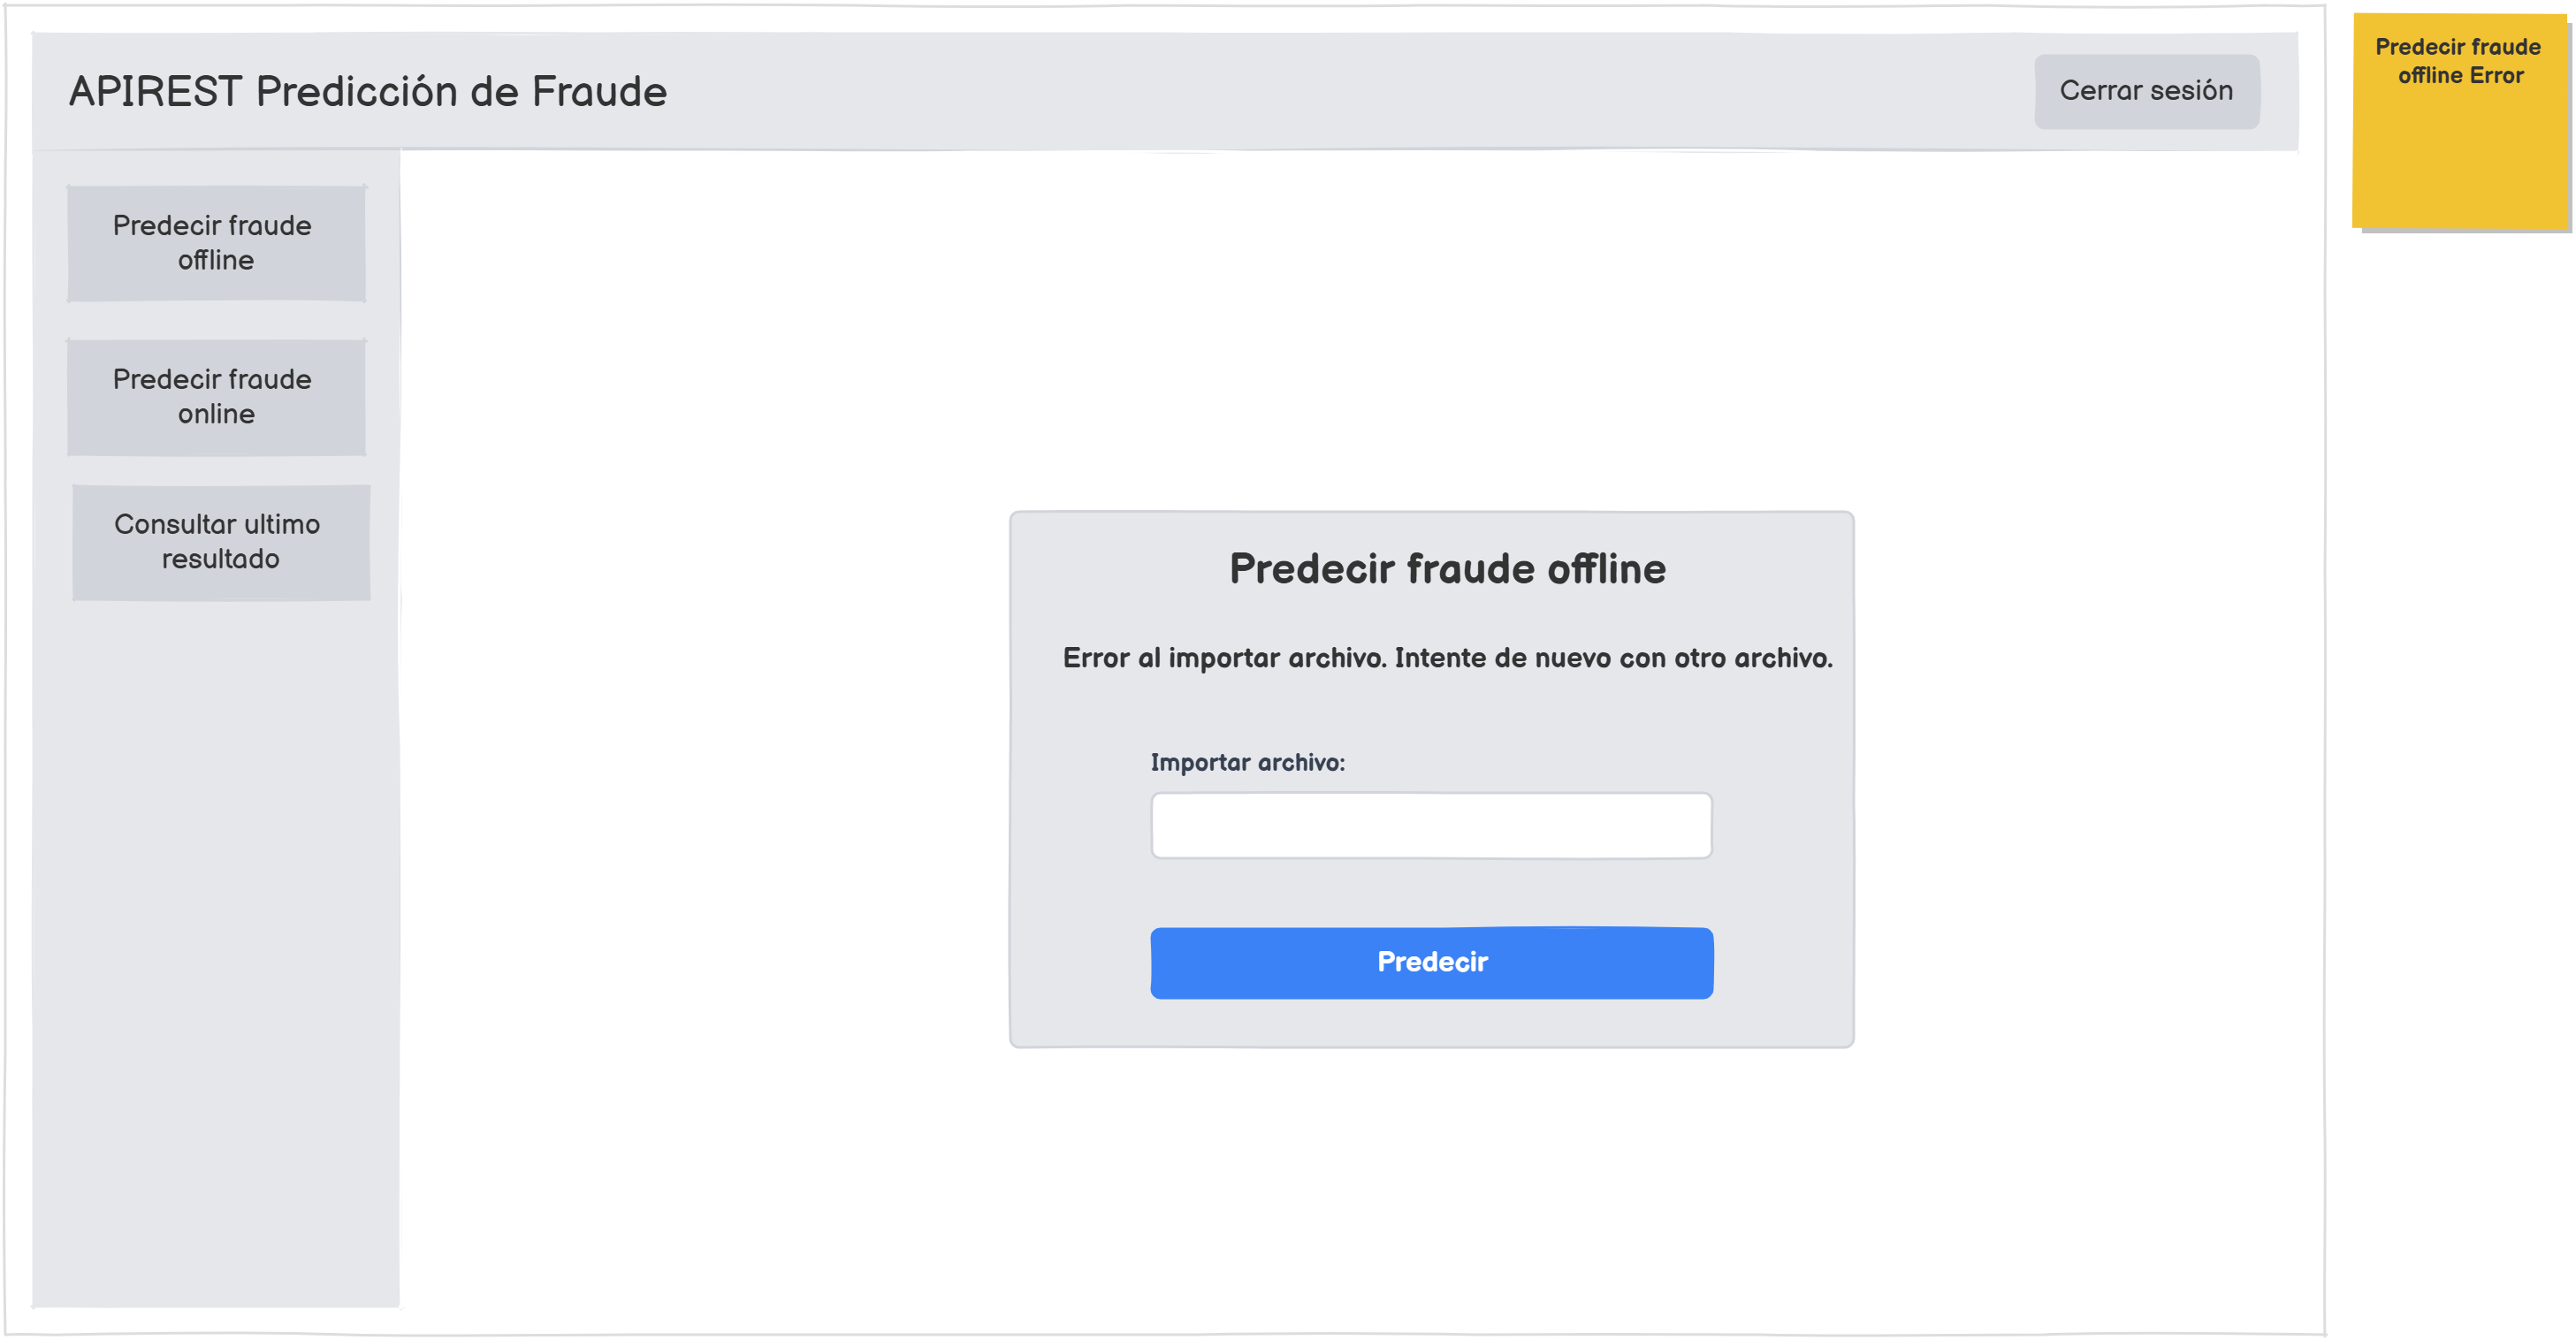
\includegraphics[width=1\textwidth]{imagenes/fraudeOfflineError_boceto.png}
\caption{Boceto de la ventana de error al predecir fraude \emph{offline}.}
\end{figure}

\begin{figure}[H]
\centering
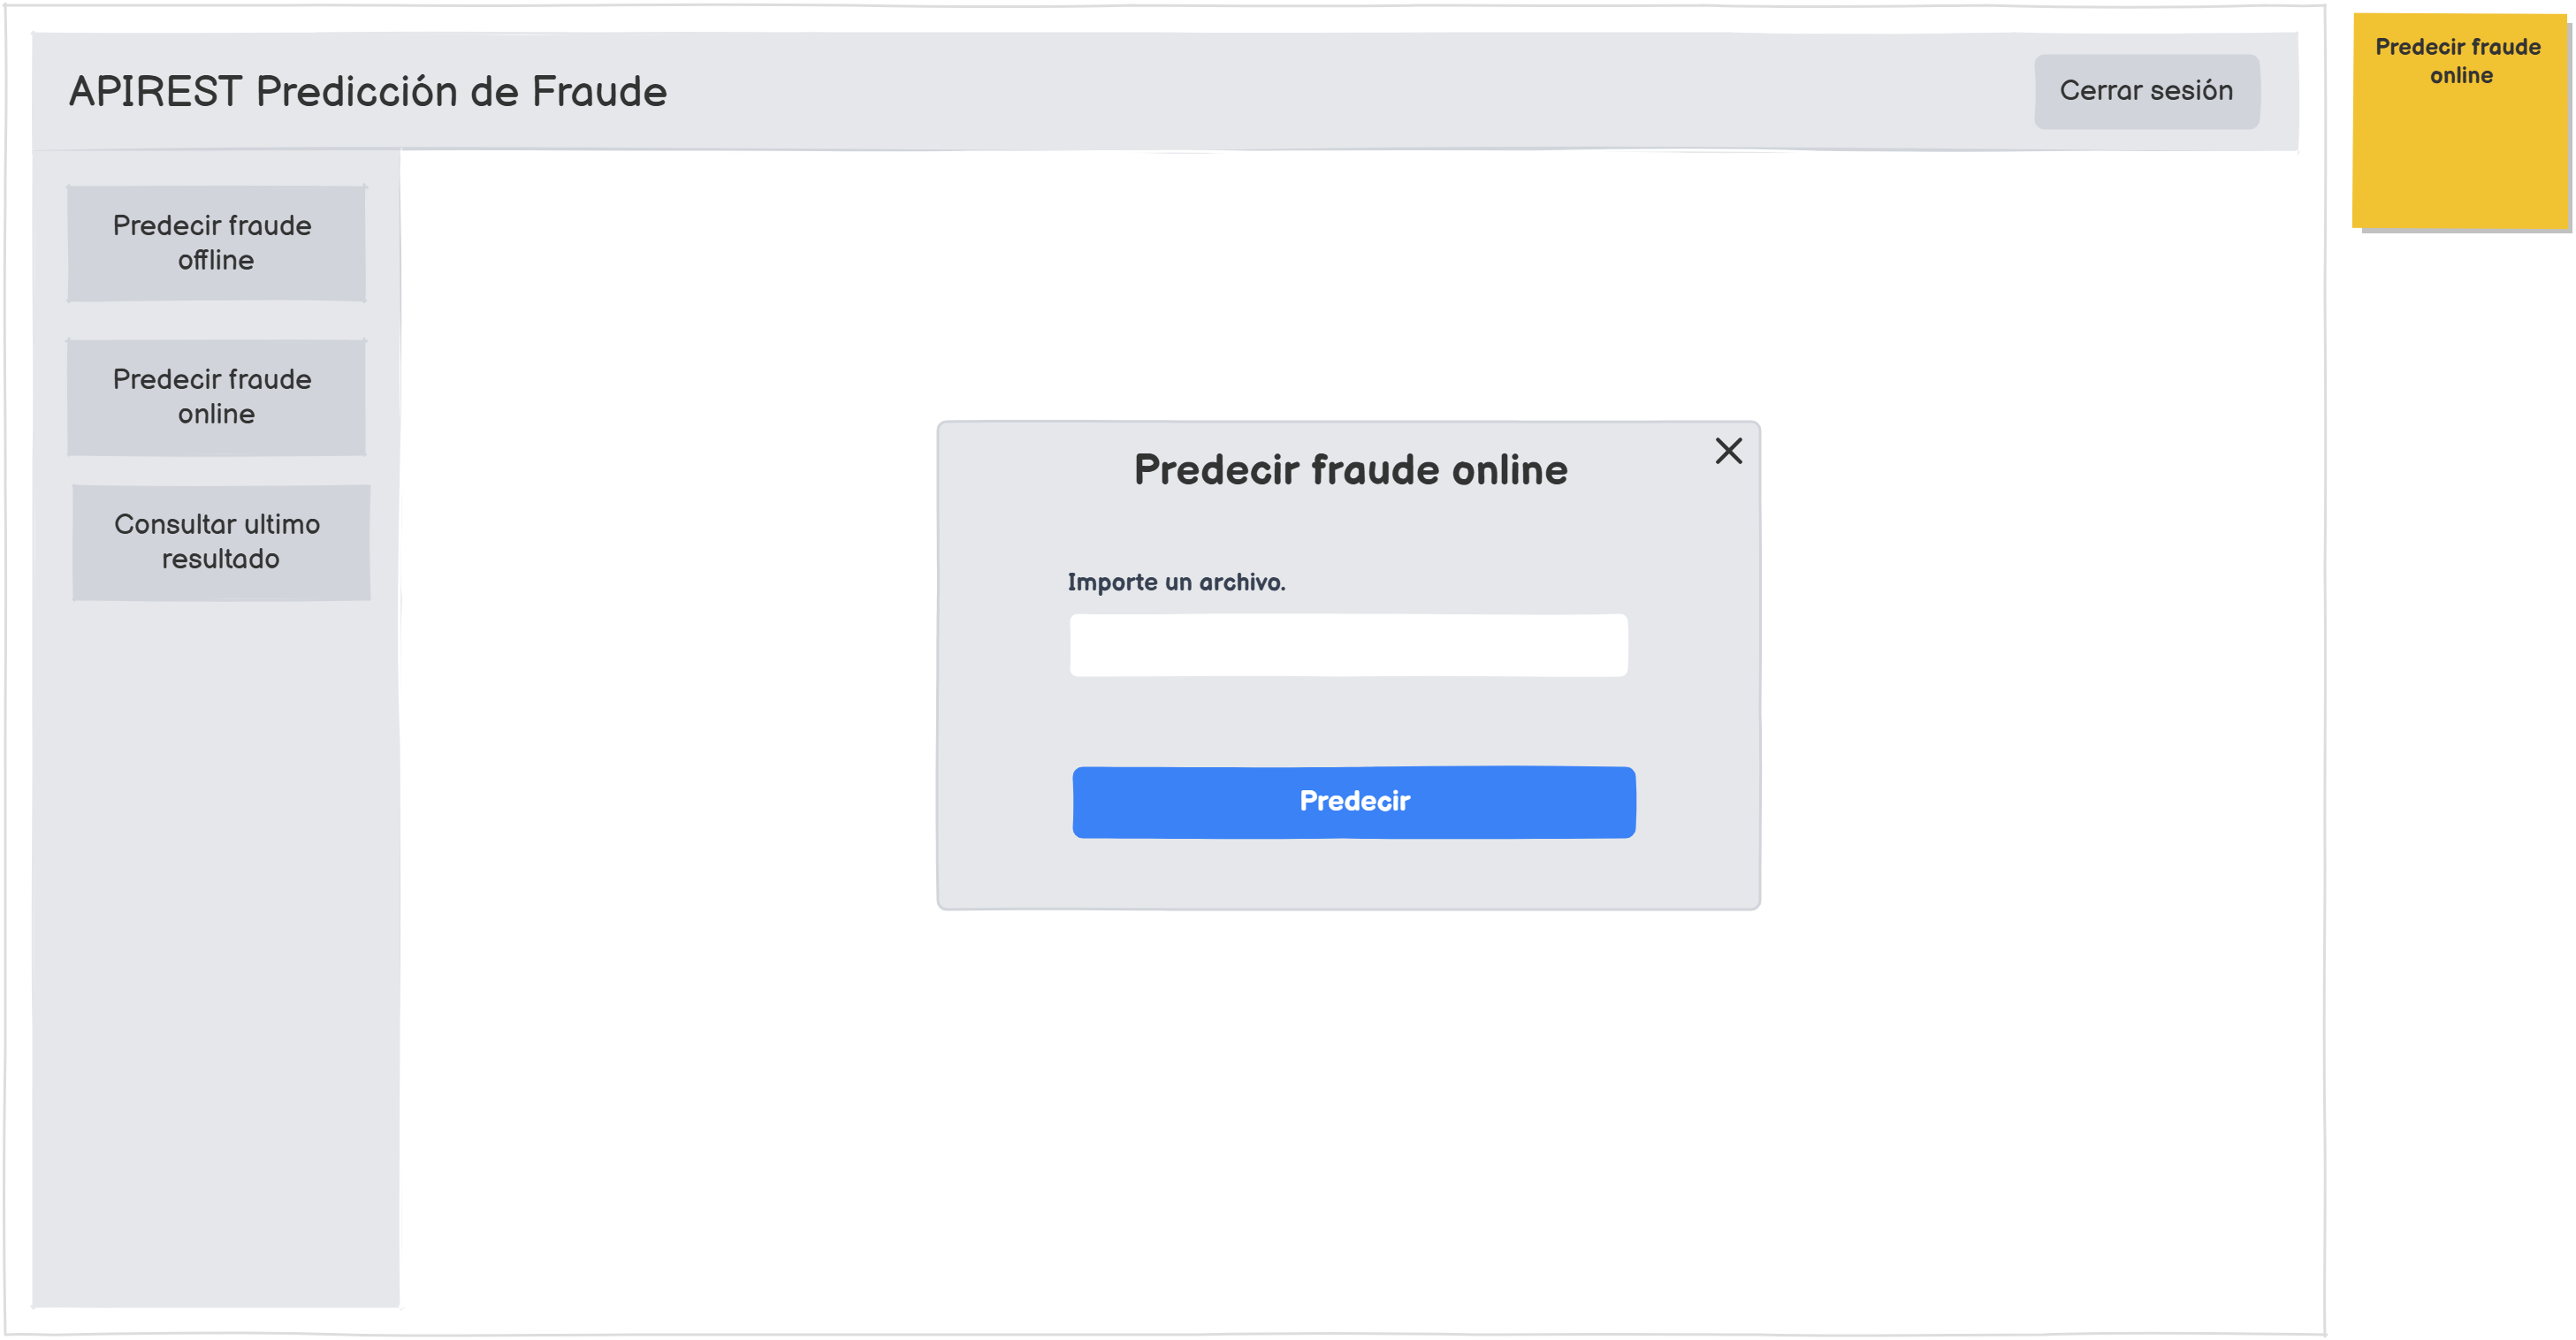
\includegraphics[width=1\textwidth]{imagenes/fraudeOnline_boceto.png}
\caption{Boceto de la ventana principal de predecir fraude \emph{online}.}
\end{figure}

\begin{figure}[H]
\centering
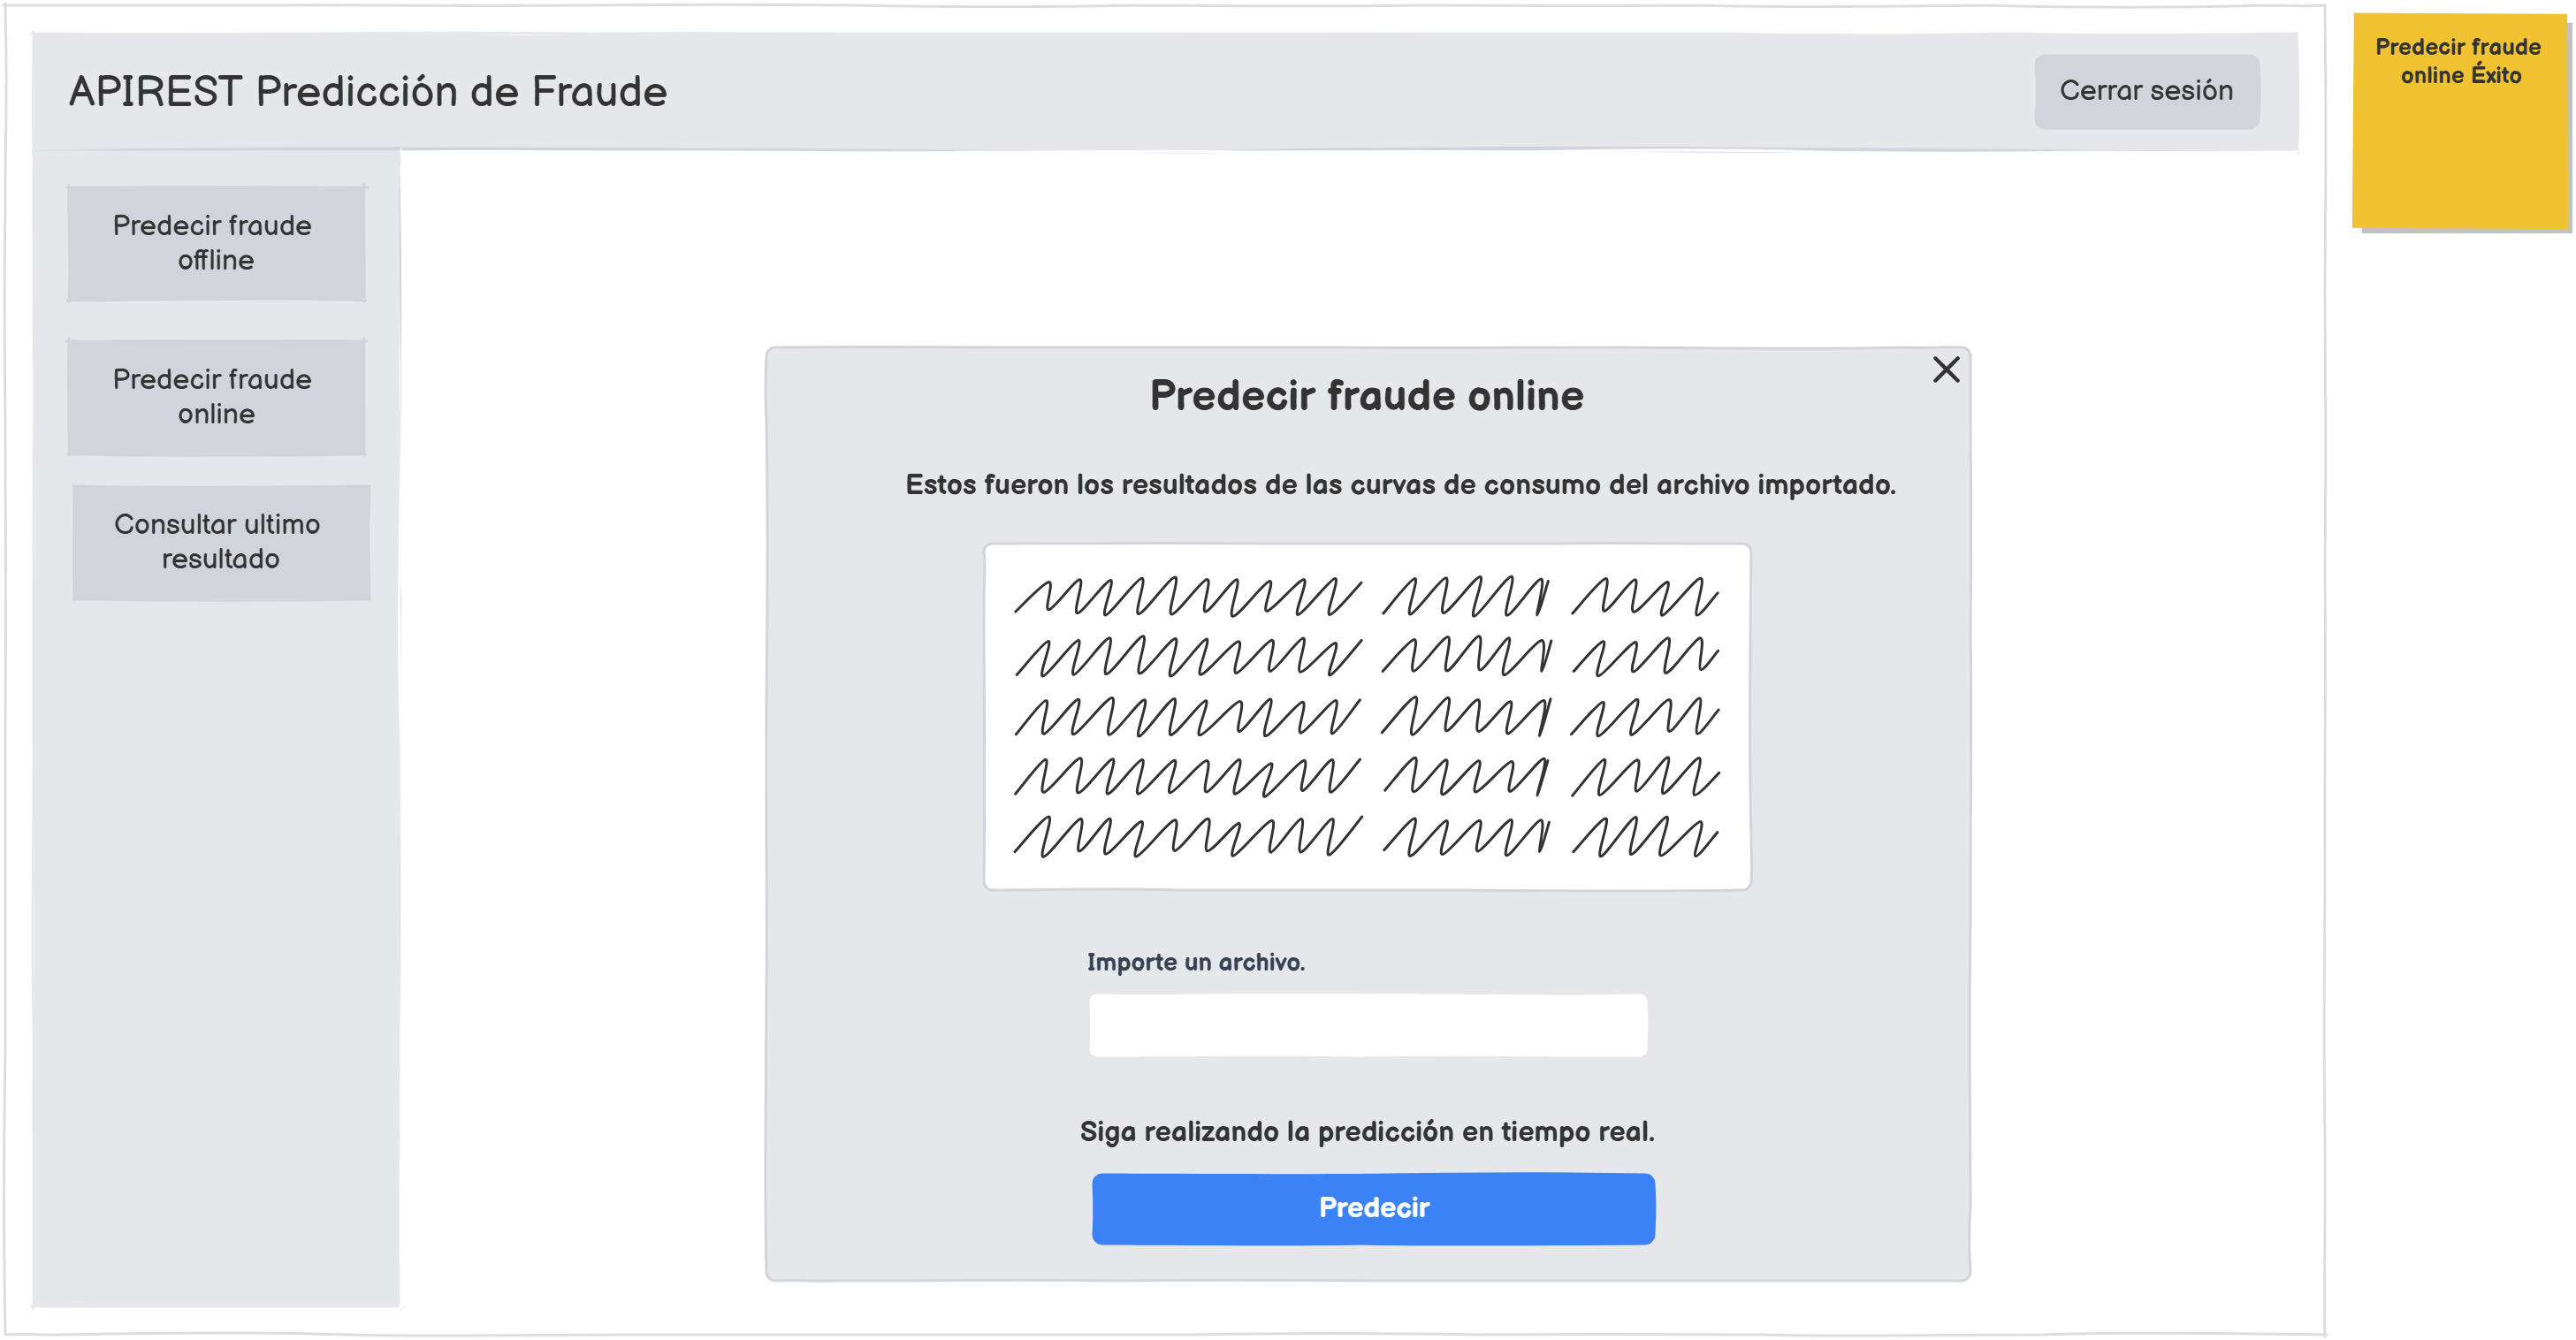
\includegraphics[width=1\textwidth]{imagenes/fraudeOnlineExito_boceto.png}
\caption{Boceto de la ventana de predecir fraude \emph{online} con éxito.}
\end{figure}

\begin{figure}[H]
\centering
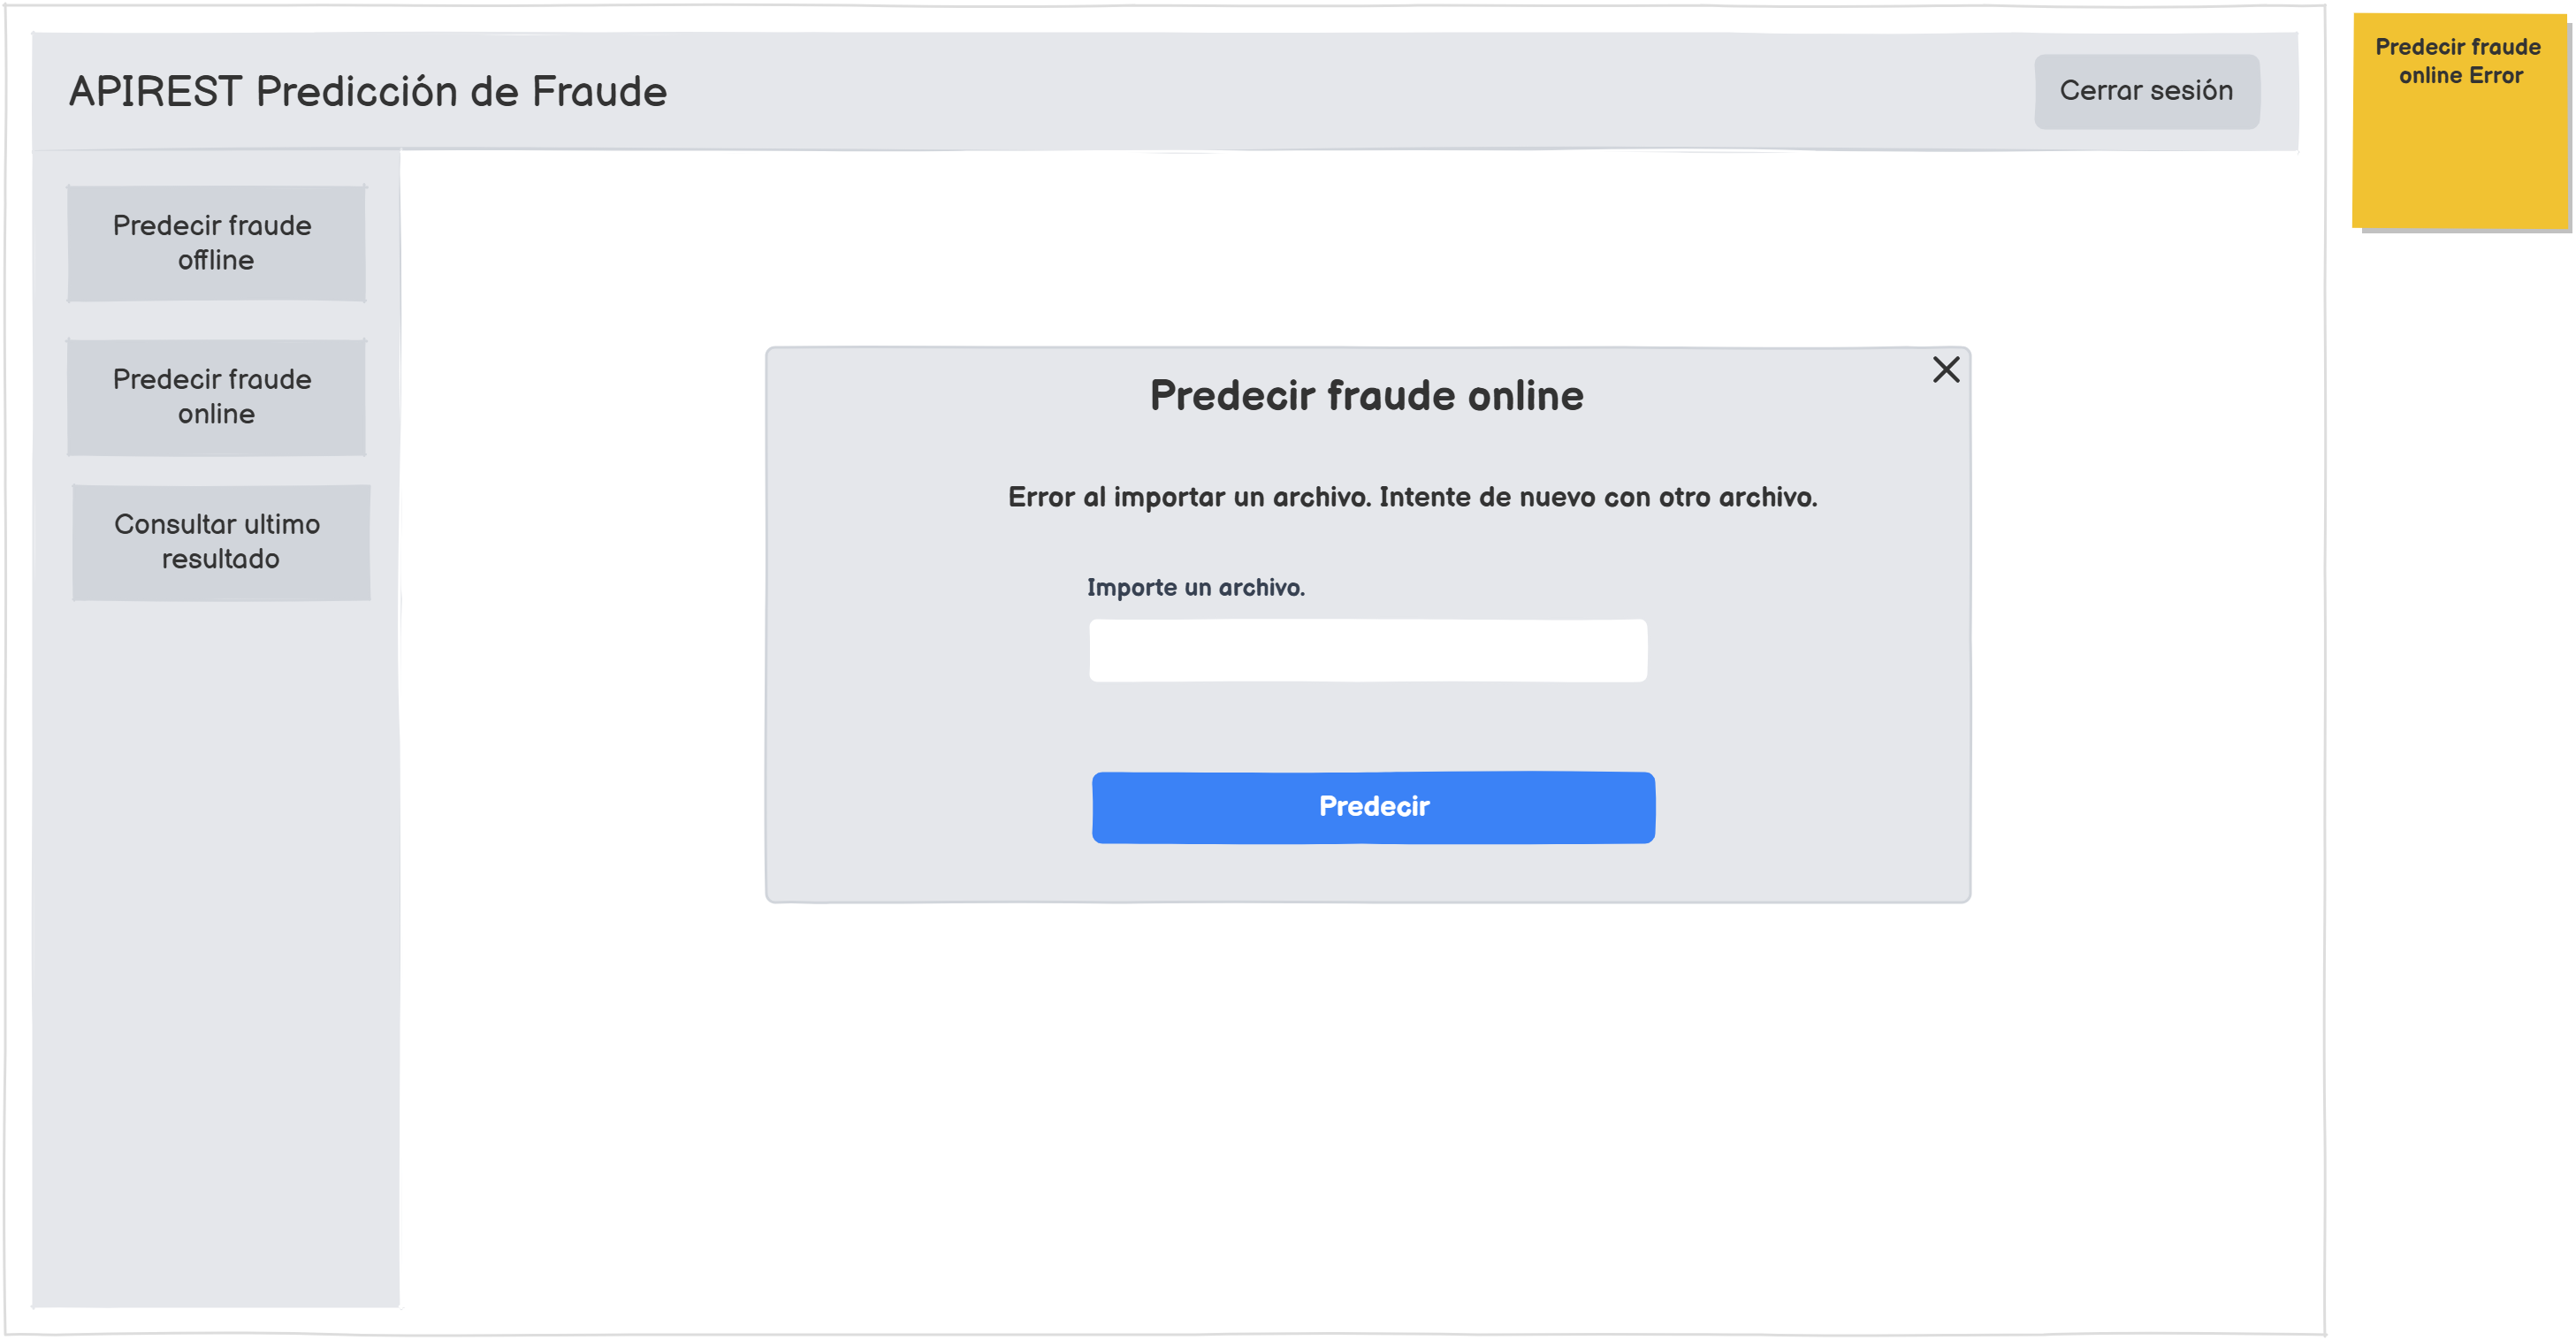
\includegraphics[width=1\textwidth]{imagenes/fraudeOnlineError_boceto.png}
\caption{Boceto de la ventana de error al predecir fraude \emph{online}.}
\end{figure}


\subsubsection{Ventanas de consulta}

Se muestran las ventanas del caso de uso de consultar último resultado de predicción junto a sus posibles errores.

\begin{figure}[H]
\centering
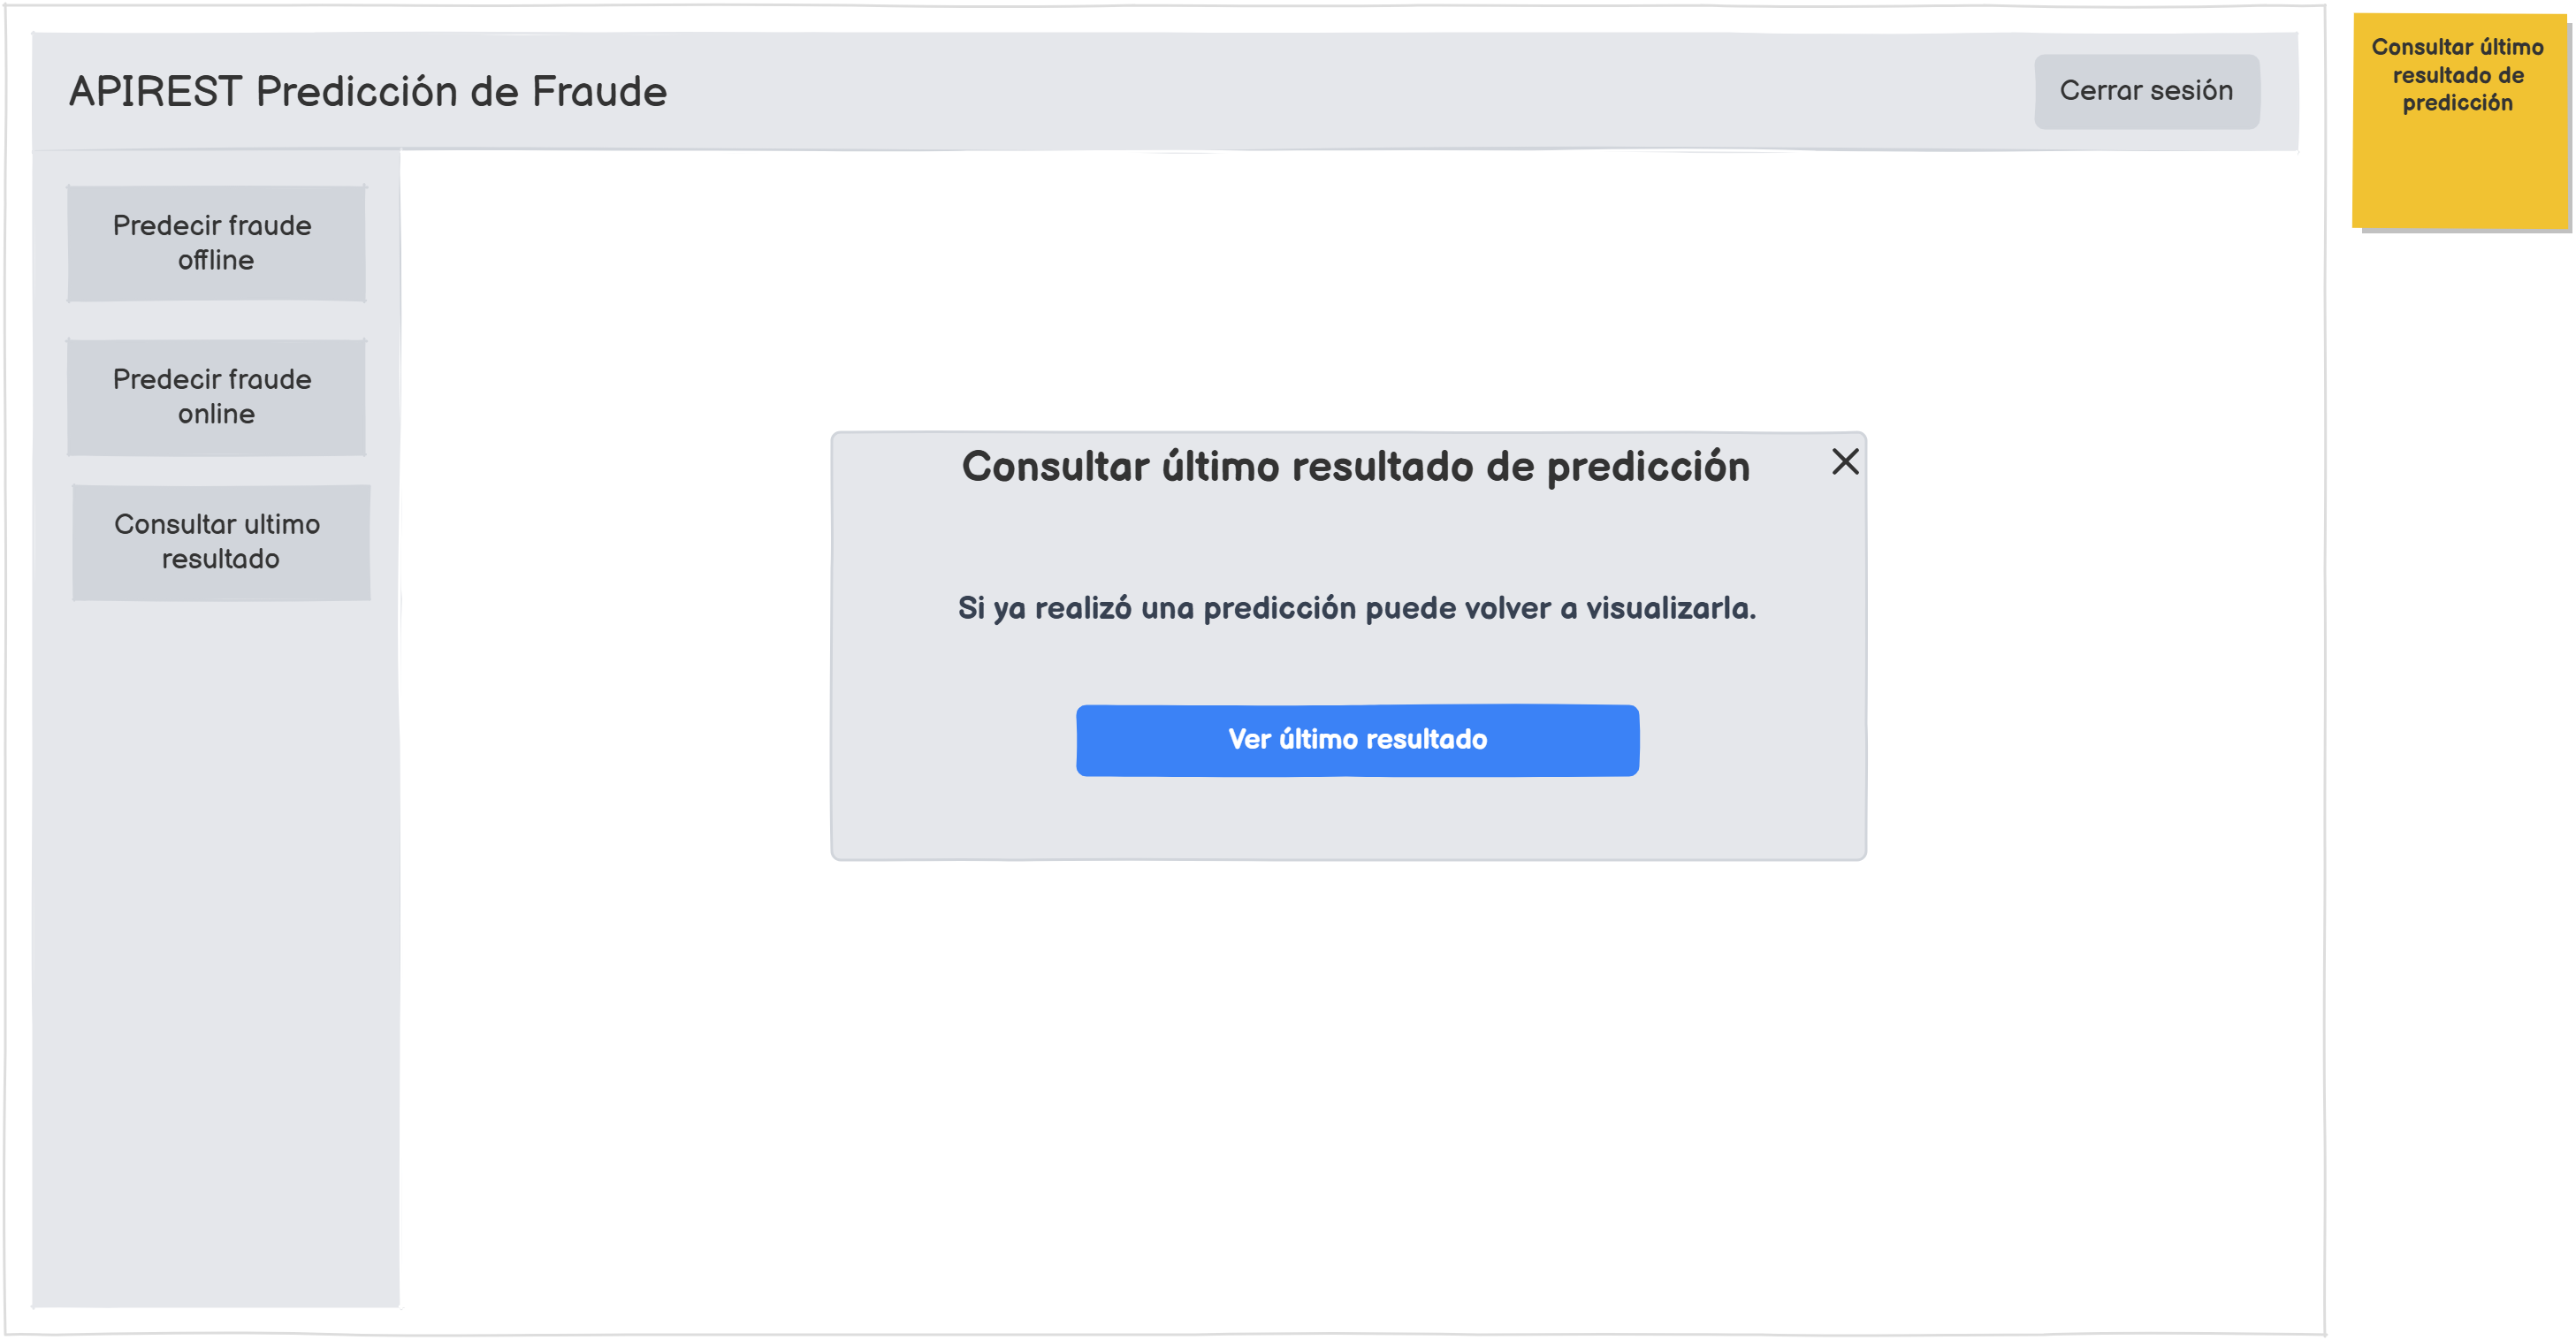
\includegraphics[width=1\textwidth]{imagenes/ultimaPrediccion_boceto.png}
\caption{Boceto de la ventana principal de consultar último resultado de predicción.}
\end{figure}

\begin{figure}[H]
\centering
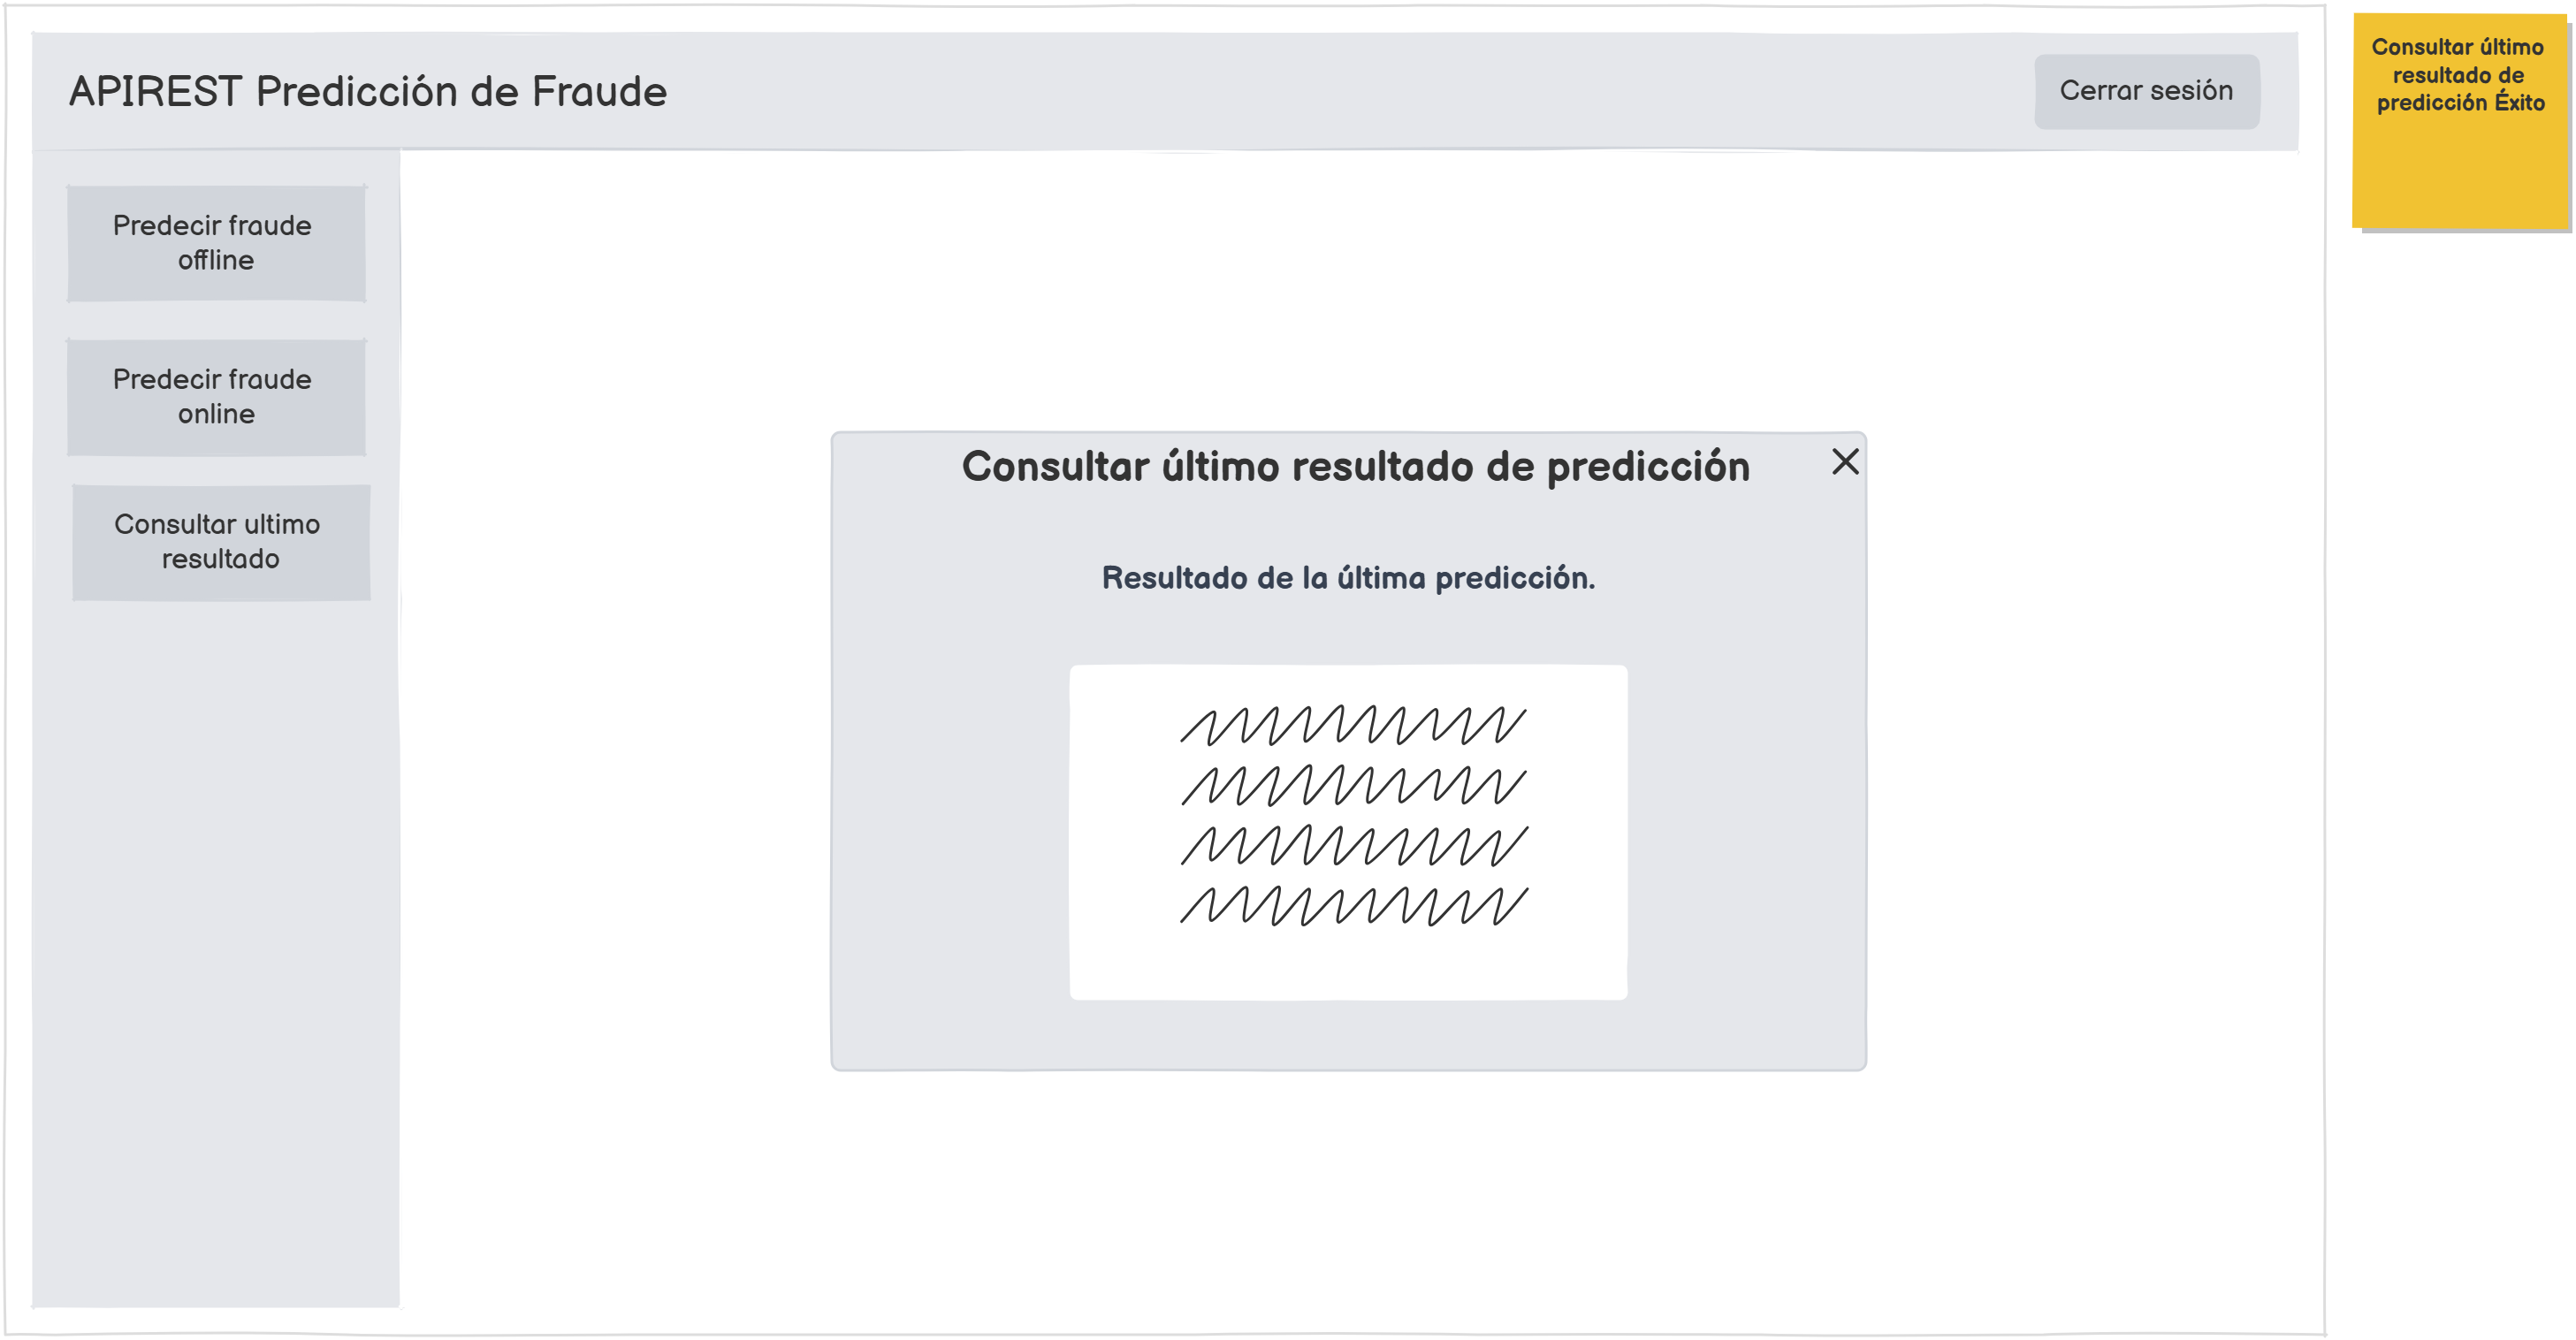
\includegraphics[width=1\textwidth]{imagenes/ultimaPrediccionExito_boceto.png}
\caption{Boceto de la ventana de consultar último resultado de predicción con éxito.}
\end{figure}

\begin{figure}[H]
\centering
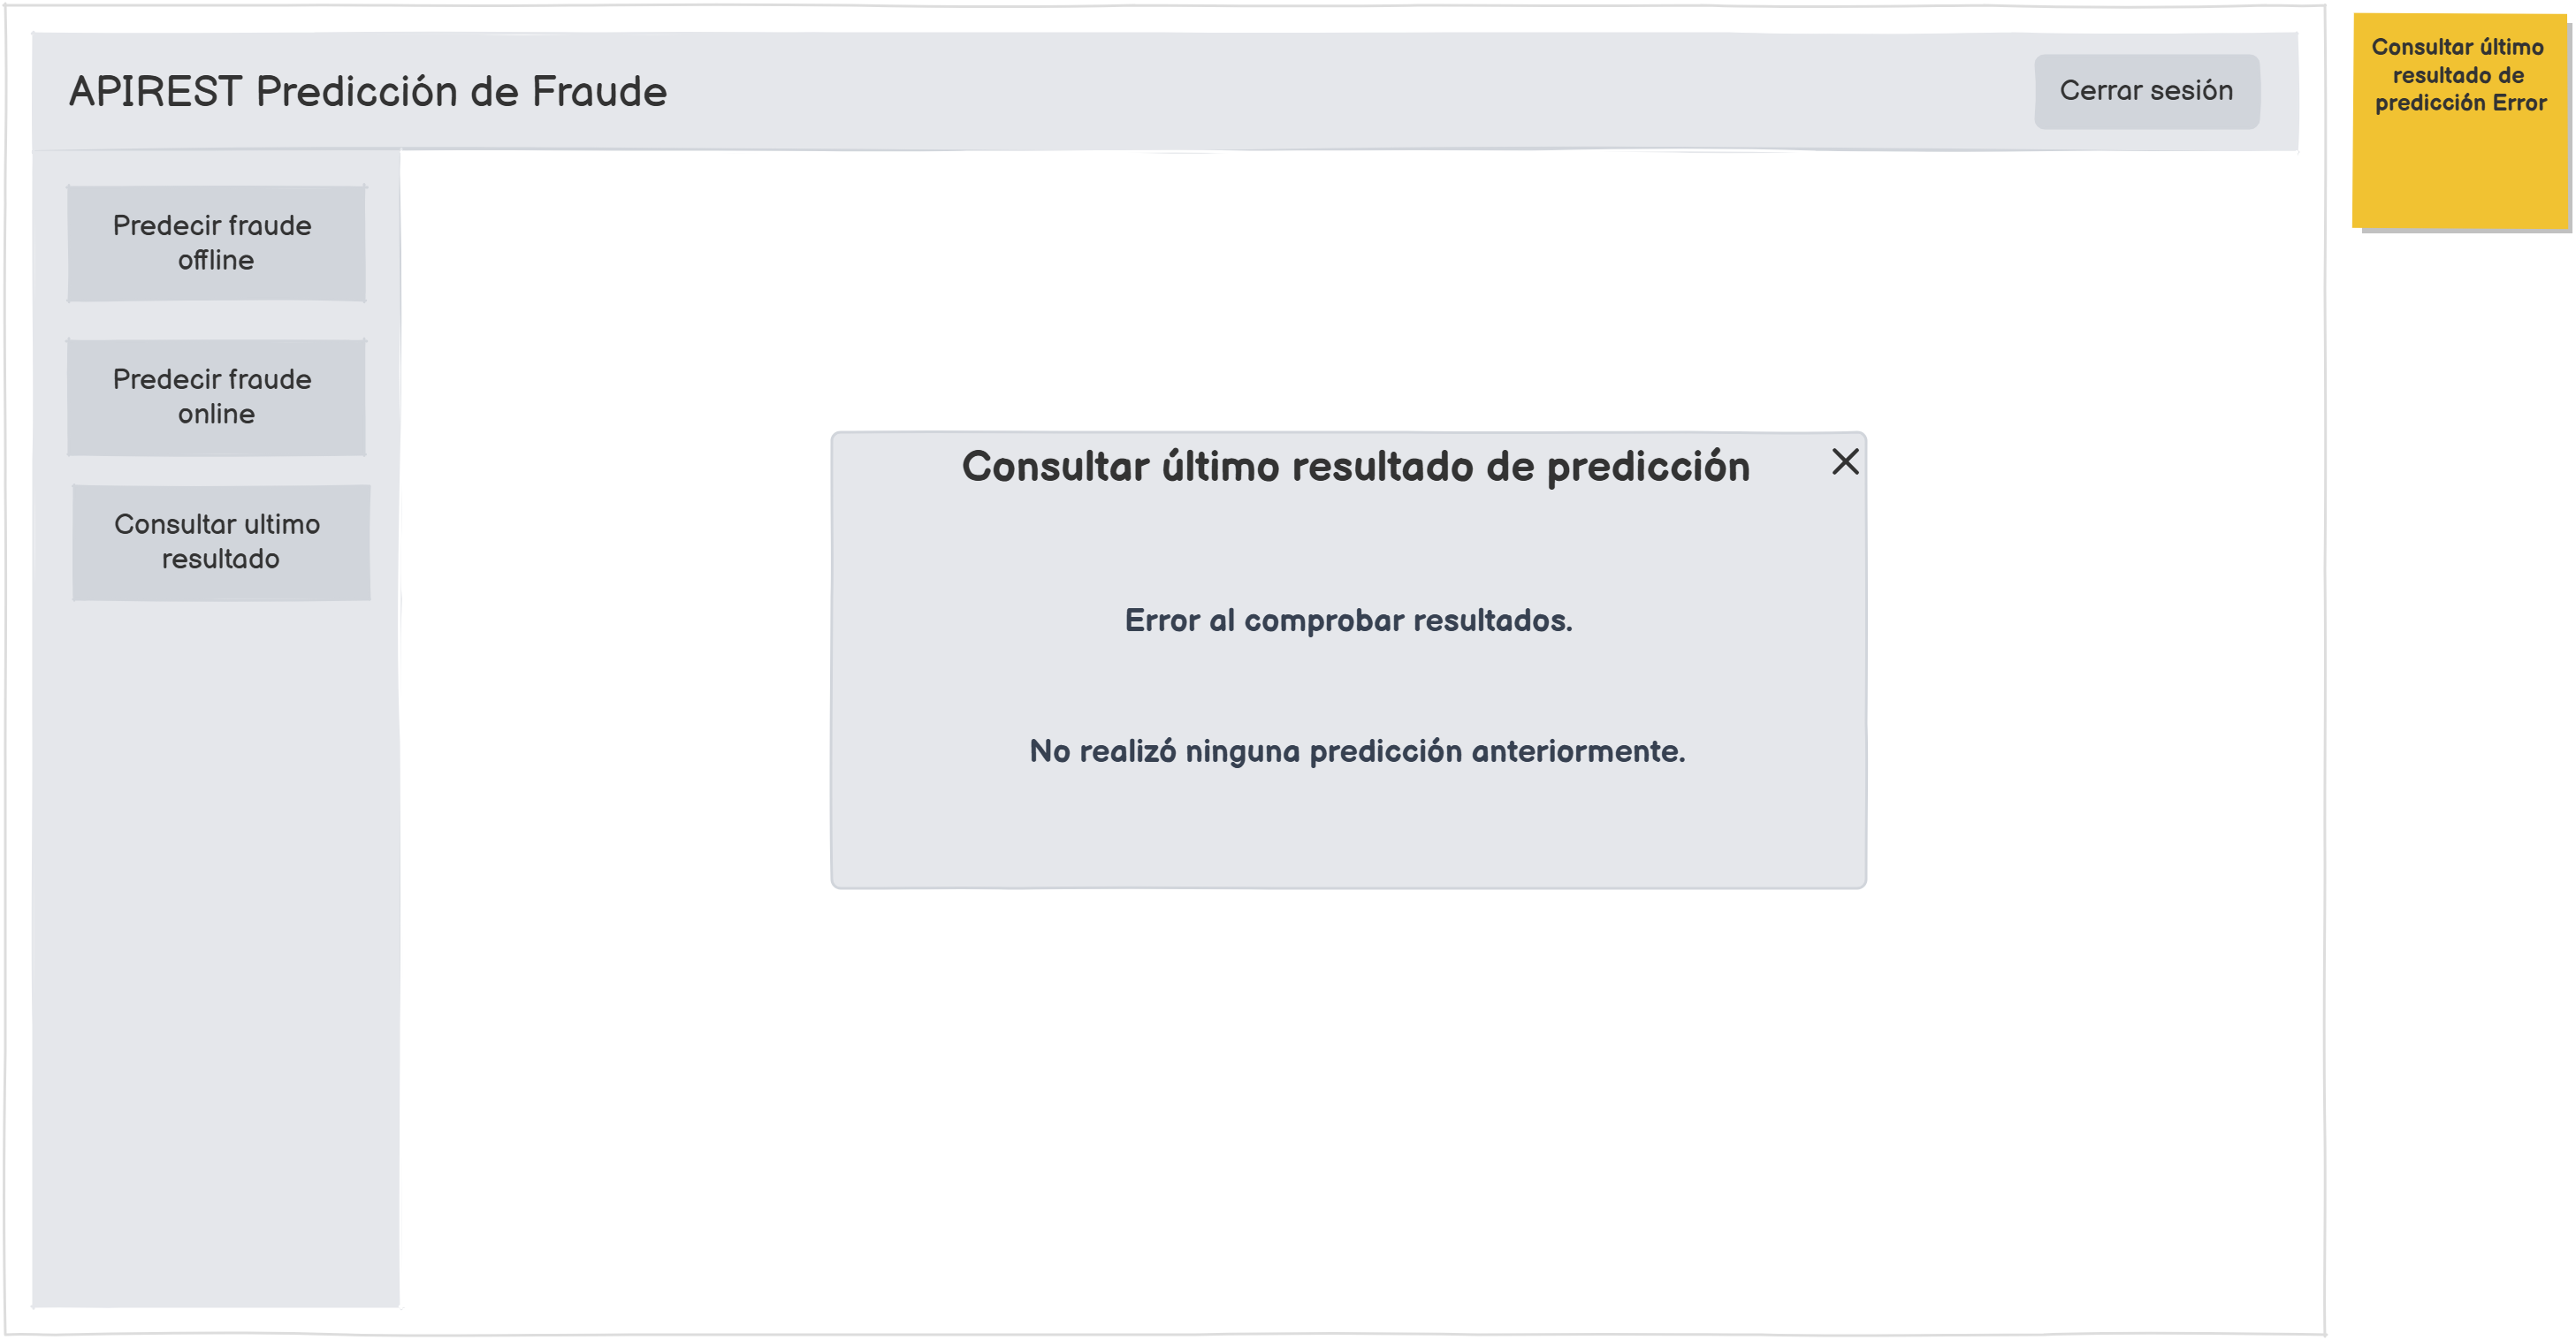
\includegraphics[width=1\textwidth]{imagenes/ultimaPrediccionError_boceto.png}
\caption{Boceto de la ventana de error al consultar último resultado de predicción.}
\end{figure}


\subsection{Diseño final}
\subsubsection{Endpoints de autenticación}
\subsubsection{Endpoints de predicción}
\subsubsection{Endpoints de consulta}


% =========================
% CAPÍTULO 10
% =========================
\chapter{Construcción del Sistema}

Este capítulo se ocupa de los elementos relacionados con la construcción del sistema de software creado. Se detalla el entorno de desarrollo que se usó, las tecnologías que se aplicaron, las resoluciones tomadas durante la creación del prototipo y la implementación a nivel de código. La aplicación \emph{back-end} ha sido creada a partir de una \emph{API REST}, la cual tiene la responsabilidad de autenticar a los usuarios, recibir archivos CSV con las curvas de consumo eléctrico, implementar los modelos predictivos escogidos en el periodo experimental y retornar los resultados al operador.


\section{Entorno de desarrollo}

El desarrollo se realiza con un equipo con \emph{Windows} junto con \emph{Python} como el lenguaje de programación principal. Esta opción es apropiada para el proyecto porque posibilita la incorporación de los modelos de aprendizaje automático que se han conseguido en la fase experimental junto con la lógica del sistema, todo dentro del mismo entorno. Se crea un entorno virtual a través de \emph{venv} para juntar las dependencias del proyecto. Las bibliotecas necesarias para la aplicación se mantienen separadas de otras instalaciones de \emph{Python} que se encuentran en el equipo, con lo cual se previenen conflictos entre versiones y se simplifica la replicación del entorno en otros equipos o en un futuro despliegue. Se ha elegido \emph{Visual Studio Code} como el entorno de desarrollo integrado, que se emplea para la edición del código fuente, la estructuración del proyecto y la ejecución de comandos en la terminal integrada. 

Para manejar e instalar las dependencias, se emplea \emph{pip}, este programa genera el archivo requirements.txt, que compila las librerías necesarias para que el sistema funcione. Durante la fase de desarrollo, la aplicación se ejecuta con \emph{Uvicorn}, un servidor \emph{ASGI} que es compatible con \emph{FastAPI}. \emph{XAMPP, phpMyAdmin} y \emph{MySQL} se utilizan para gestionar la base de datos. Esto permite crear y gestionar una base de datos de los usuarios del sistema, donde se encuentran los roles, el estado de activación y la información de autenticación. Finalmente, se utiliza \emph{Git} para controlar las versiones, lo que permite llevar un registro del progreso del código fuente y supervisar los cambios realizados durante la construcción del sistema.


\section{Tecnologías utilizadas}

Para construir el sistema se emplean diversas tecnologías en las que cada una se encarga de una tarea distinta. Se emplea \emph{FastAPI} como base fundamental para crear la \emph{API REST}. Esta aporta que los \emph{endpoints} funcionen y hagan su tarea correctamente, la validación de los parámetros de entrada y la creación automática de una documentación del sistema que es interactiva. Garcias a esto el operador puede comprobar las funcionalidades disponibles a través de una interfaz a la que se accede por medio del navegador. La aplicación desarrollada con \emph{FastAPI} se ejecuta usando el servidor \emph{ASGI} llamado \emph{Uvicorn}. Este servidor permite atender las peticiones HTTP recibidas por la API y ejecutar los endpoints definidos en el sistema.

Para la lectura, manipulación y preprocesamiento de los archivos CSV importados por el operador se utiliza\emph{Pandas}. Esta se encarga de cargar las curvas de consumo, eliminar columnas innecesarias, adaptar las variables al formato requerido por los modelos y preparar los datos antes de realizar la predicción. Para la predicción sobre consumo histórico se ha utilizado el modelo \emph{XGBoost}, implementado mediante la biblioteca \emph{xgboost} de \emph{Python}. Este se selecciona como mejor técnica \emph{offline} durante la fase experimental y se integra en el sistema para clasificar archivos completos de curvas de consumo. Para la predicción en tiempo real se ha utilizado el modelo \emph{Adaptive Random Forest}, implementado mediante la biblioteca \emph{River}, orientada al aprendizaje automático online. Este modelo permite clasificar los registros de forma secuencial dentro de la simulación de flujo en tiempo real. También, se utiliza \emph{Scikit-learn} como biblioteca auxiliar en determinados procesos asociados a los modelos, especialmente en el escalado de datos necesario para mantener la coherencia entre la fase experimental y la fase operativa del sistema.

Se emplea \emph{MySQL} como sistema gestor de base de datos para administrar usuarios. Se guardan los datos necesarios para la autenticación. La \emph{API} y la base de datos se comunican mediante \emph{PyMySQL}, lo que permite realizar consultas a través del código Python. Para una buena seguridad en las contraseñas se emplea \emph{hash} mediante el algoritmo \emph{bcrypt} y la biblioteca \emph{Passlib}. Estos ayudan a la verificación de las contraseñas que el usuario ingresa, al compararlas con el hash guardado en la base de datos. Así, se evita almacenar las contraseñas como texto plano.

Se utiliza \emph{Pickle}, módulo estándar de \emph{Python}, para cargar recursos generados previamente durante la fase experimental, como modelos entrenados, listas de columnas esperadas y escaladores. Esto hace que la aplicación utilice los modelos ya entrenados sin necesidad de repetir el proceso de entrenamiento durante el uso del sistema. El uso de todas estas tecnologías permite construir un sistema modular, capaz de integrar modelos de aprendizaje automático previamente entrenados dentro de una \emph{API REST} protegida mediante autenticación y preparada para realizar predicciones sobre nuevas curvas de consumo eléctrico.


\section{Implementación de la API REST}


\subsection{Implementación de endpoints}


\subsection{Integración de resultados experimentales}


\section{Documentación interactiva con Swagger UI}


\section{Código fuente y modularidad}


\section{Control de versiones}


\section{Despliegue del sistema}



% =========================
% CAPÍTULO 11
% =========================
\chapter{Validación del Sistema}


\section{Estrategia de validación}


\section{Pruebas funcionales}


\section{Pruebas no funcionales}


\section{Pruebas de rendimiento}


\section{Validación global del prototipo}



% =========================
% PARTE III EPÍLOGO
% =========================
\part{Epílogo}


% =========================
% CAPÍTULO 12
% =========================
\chapter{Conclusiones}


\section{Objetivos alcanzados}


\section{Lecciones aprendidas}


\section{Trabajo futuro}


% =========================
% PARTE IV ANEXO
% =========================
\part{Anexo}


% =========================
% CAPÍTULO 13
% =========================
\chapter{Dependencias y paquetes Python}


% =========================
% CAPÍTULO 14
% =========================
\chapter{Manual de usuario}


\section{Introducción}


\section{Uso del sistema}


\subsection{Consulta de modelos offline}


\subsection{Consulta de modelos online}


\subsection{Obtención del mejor modelo}


\subsection{Visualización de curvas ROC}


\subsection{Lectura de respuestas JSON}


\cleardoublepage
\addcontentsline{toc}{chapter}{Bibliografía}
\begin{thebibliography}{9}

\bibitem{endesa}
Endesa. Fraude eléctrico: cómo actuar. 
Disponible en: \url{https://www.endesa.com/es/la-cara-e/red-electrica/fraude-electico-como-actuar}

\bibitem{articulo1}
Evaluation of Online Machine Learning Algorithms for Electricity Theft Detection in Smart Grids. 
Disponible en: \url{https://www.researchgate.net/publication/364956749_Evaluation_of_Online_Machine_Learning_Algorithms_for_Electricity_Theft_Detection_in_Smart_Grids}

\bibitem{articuloAnálisisRedEléctrica}
Electricity Theft Detection in Smart Grid Systems. 
Disponible en: \url{https://engineering.case.edu/sites/default/files/chinacom14.pdf}

\bibitem{articuloBase}
Electricity Theft Detection: A Comparative Study of Different Approaches. 
Disponible en: \url{https://ieeexplore.ieee.org/abstract/document/9612408}

\bibitem{articuloRedEléctrica}
Power flow state estimation using Newton algorithm. 
Disponible en: \url{https://d197for5662m48.cloudfront.net/documents/publicationstatus/243171/preprint_pdf/59f25b2ab75f10bf828cd6770d8d676d.pdf}

\bibitem{ML Supervisado}
¿Qué es el aprendizaje supervisado? 
Disponible en: \url{https://www.ibm.com/es-es/think/topics/supervised-learning}

\bibitem{ML No Supervisado}
¿Qué es el aprendizaje no supervisado? 
Disponible en: \url{https://www.ibm.com/es-es/think/topics/unsupervised-learning}

\bibitem{ML Semisupervisado}
¿Qué es el aprendizaje semisupervisado? 
Disponible en: \url{https://www.ibm.com/es-es/think/topics/semi-supervised-learning}

\bibitem{dataset}
Theft Detection Dataset (TDD2022). 
Mendeley Data. 
Disponible en: \url{https://data.mendeley.com/datasets/c3c7329tjj/1}

\bibitem{articulo2}
Theft detection dataset for benchmarking and machine learning based classification in a smart grid environment. 
Disponible en: \url{https://www.sciencedirect.com/science/article/pii/S1319157822001562}

\bibitem{articulo3}
Dynamic electricity theft behavior analysis based on active learning and incremental learning in new power systems. 
Disponible en: \url{https://www.sciencedirect.com/science/article/pii/S0142061524005325}

\bibitem{articulo4}
A Hoeffding D Statistic Approach for Detecting Electricity Theft. 
Disponible en: \url{https://www.researchgate.net/publication/385234208_A_Hoeffding_D_Statistic_Approach_for_Detecting_Electricity_Theft}

\bibitem{articulo5}
Suspicious Electric Consumption Detection Based on Multi-Profiling Using Live Machine Learning. 
Disponible en: \url{https://jacquesklein2302.github.io/papers/2015-SmartGridComm15-author-preprint-20151104.pdf}

\bibitem{randstad}
Randstad. 
¿Cuánto cobra un ingeniero informático en España? 
Disponible en: \url{https://www.randstad.es/contenidos360/orientacion-laboral/cuanto-cobra-un-ingeniero-informatico-en-espana/#sueldo-ingeniero-informatico-segun-experiencia}

\bibitem{tradespark_ml}
TradeSpark. \textit{Python for AT: Machine Learning}. Disponible en: 
\url{https://tradespark.la/blog/articulos/python-for-at/machine-learning/}. 

\bibitem{logistic-regression}
¿Qué es la regresión logística?
Disponible en: \url{https://aws.amazon.com/es/what-is/logistic-regression/}

\bibitem{Random Forest}
¿Bosques aleatorios?
Disponible en: \url{https://www.ibm.com/mx-es/think/topics/random-forest}

\bibitem{Gradient Boosting}
¿Qué es el Gradient Boosting?
Disponible en: \url{https://www.ibm.com/es-es/think/topics/gradient-boosting}

\bibitem{Perceptrón Multicapa}
Perceptrón multicapa
Disponible en: \url{https://www.datacamp.com/es/tutorial/multilayer-perceptrons-in-machine-learning}

\bibitem{k-Nearest Neighbors}
¿Qué es el algoritmo de k vecinos más cercanos (KNN)?
Disponible en: \url{https://www.ibm.com/mx-es/think/topics/knn}

\bibitem{XGBoost}
¿Qué es XGBoost?
Disponible en: \url{https://www.ibm.com/mx-es/think/topics/xgboost}

\bibitem{Perceptrón}
Perceptrón.
Disponible en: \url{https://es.wikipedia.org/wiki/Perceptr%C3%B3n}

\bibitem{Naive Bayes incremental}
Naive Bayes.
Disponible en: \url{https://www.ibm.com/es-es/think/topics/naive-bayes}

\bibitem{Hoeffding Tree}
Hoeffding Tree Classifier.
Disponible en: \url{https://docs.turboml.com/classification/hoeffdingtreeclassifier/}

\bibitem{Hoeffding Tree Implementation}
Hoeffding Tree Classifier Implementation.
Disponible en: \url{https://riverml.xyz/dev/api/tree/HoeffdingTreeClassifier/}

\bibitem{Adaptive Random Forest}
Adaptive Random Forest.
Disponible en: \url{https://moa.cms.waikato.ac.nz/adaptive-random-forest/}

\bibitem{Métricas ML}
¿Qué es una métrica en Machine Learning?
Disponible en: \url{https://liora.io/es/metricas-en-machine-learning}

\bibitem{F1-score}
Puntuación F1 en aprendizaje automático.
Disponible en: \url{https://www.datacamp.com/tutorial/f1-score}

\bibitem{Matriz de confusión}
¿Qué es una matriz de confusión?
Disponible en: \url{https://www.ibm.com/es-es/think/topics/confusion-matrix}

\bibitem{Coeficiente Kappa}
¿Qué es el kappa de Cohen?
Disponible en: \url{https://www.knime.com/blog/cohens-kappa-an-overview#:~:text=expected%20prediction%20accuracy-,Why%20it%20happens,many%20predictions%20will%20be%20right.%E2%80%9D}

\bibitem{Tasa de Falsos Positivos}
False Positive Rate
Disponible en: \url{https://interactivechaos.com/es/manual/tutorial-de-machine-learning/false-positive-rate}

\bibitem{ROC-AUC}
AUC y Curva ROC en Aprendizaje Automático
Disponible en: \url{https://www.datacamp.com/es/tutorial/auc}

\bibitem{Regresión Logística Python}
Logistic Regression
Disponible en: \url{https://scikit-learn.org/stable/modules/generated/sklearn.linear_model.LogisticRegression.html#sklearn.linear_model.LogisticRegression}

\bibitem{Random Forest Python}
Random Forest Classifier
Disponible en: \url{https://scikit-learn.org/stable/modules/generated/sklearn.ensemble.RandomForestClassifier.html}

\bibitem{Gradient Boosting Python}
Gradient Boosting Classifier
Disponible en: \url{https://scikit-learn.org/stable/modules/generated/sklearn.ensemble.GradientBoostingClassifier.html}

\bibitem{MLP Python}
Multi-layer Perceptron
Disponible en: \url{https://scikit-learn.org/stable/modules/neural_networks_supervised.html}

\bibitem{k-Nearest Neighbors Python}
Nearest Neighbors
Disponible en: \url{https://scikit-learn.org/stable/modules/neighbors.html}

\bibitem{XGBoost Python}
XGBoost Python Package
Disponible en: \url{https://xgboost.readthedocs.io/en/stable/python/python_intro.html}

\bibitem{Perceptrón Python}
Perceptron Python Package
Disponible en: \url{https://scikit-learn.org/stable/modules/generated/sklearn.linear_model.Perceptron.html}

\bibitem{Naive Bayes Python}
Naive Bayes Python Package
Disponible en: \url{https://scikit-learn.org/stable/modules/naive_bayes.html}

\bibitem{Hoeffding Tree Python}
Hoeffding Tree Python Package
Disponible en: \url{https://medium.com/we-talk-data/a-beginners-guide-to-hoeffding-tree-with-python-implementation-64bb90b5a91c}

\bibitem{Adaptive Random Forest Python}
Adaptive Random Forest Python Package
Disponible en: \url{https://scikit-learn.org/stable/modules/generated/sklearn.ensemble.RandomForestRegressor.html}


\end{thebibliography}


\end{document}
